%%!TEX encoding = UTF-8 Unicode

% Several lines in file have comments suggesting common packages for the
% typical thesis in informatics or electronics developed at UA
% uncomment/comment the lines as required for your work
% Before each optional line you will have a small comment

% According to UA rules, font size should range from 10 to 12pt.
\documentclass[11pt,a4paper,oneside,onecolumn]{memoir}

\listfiles
%\fixpdflayout

\usepackage[utf8]{inputenc}

% Select Computer Modern Typewritter (For bold ttfamily in listings)
\usepackage{lmodern}
% OR... Bera Mono
%\usepackage[scaled]{beramono} % TTT Font
%\usepackage{anyfontsize} % As the name says...

\usepackage[T1]{fontenc}

% Enable for for Overleaf support
\usepackage{ifthen}
\def\useoverleaf{1}  % change to non-zero (for instance, 1) to enable it

\makeatletter
\newcommand{\makecoverfile}[0]{%
  \immediate\write18{latexmk -pdf cover.tex}%
}
\makeatother

% For PDF merging
\usepackage{pdfpages}

% Set DPI to 300
\pdfpxdimen=\dimexpr 1in/300\relax

% Allow the use of a larger number of packages
\usepackage{morewrites} 

% For English and Portuguese languages
% Portuguese will be the default.
% Uncomment \setlanguage below to change it
\usepackage[english,portuguese]{babel}

% Uncomment to use a custom date format
%\usepackage{datetime}
%\newdateformat{thesisdate}{\monthname[\THEMONTH] \THEYEAR} % Month Year

% Make pdf look better
\usepackage{microtype} 

% Uncomment to enable floats on facing pages
%\usepackage{dpfloat}

% Side by side figures
% Eg. Fig 1a, Fig 1b
\usepackage[hang,small,bf]{caption}
%\let\tion\undefined
%\let\subfloat\undefined
\usepackage{subcaption}

%\RequirePackage{textcase}

% Dropped Caps
%\usepackage{lettrine}

% Configure Hyperlink color
% As a matter or style, you may use this to enable/disable color boxes on links
%\usepackage[breaklinks=true,colorlinks=false,linkcolor=blue]{hyperref}
% Or use the default values provided by the hyperref package
\usepackage{hyperref}

% Redefine section names according to your preference
%\def\sectionautorefname{Section}
%\def\chapterautorefname{Chapter}
%\def\figureautorefname{Figure}
%\def\listingautorefname{Listing}
%\def\tableautorefname{Table}

% Redefine code boxes
\ifthenelse{\equal{\useoverleaf}{0}}
{\usepackage[outputdir=build]{minted}}
{\usepackage{minted}}%

\addto\captionsportuguese{%
  \renewcommand\listingscaption{Código}
}
\fvset{fontsize=\footnotesize} % Make Code blocks smaller than text
\usepackage{csquotes}

% Add support for PDF Comments
\usepackage{comment}
\ifthenelse{\equal{\useoverleaf}{0}}
{\usepackage{pdfcomment}}{}
\usepackage{bookmark} % New Bookmarks

% For Multiple columns in Glossary
\usepackage{multicol}

% Add support for Math symbols
\usepackage{amsmath}
\usepackage{amssymb}

% Add support for graphics
\usepackage{graphicx}

% Add support for Colors
\usepackage{xcolor}

% Add support for the Euro symbol
\usepackage{eurosym}

% Add support for missingfigure and todo
\usepackage{todonotes}

% Setup bibliography with Biber using IEEE style for proper UTF-8 support
\usepackage[backend=biber, style=ieee, sorting=none, natbib=true, mincitenames=1, maxcitenames=2]{biblatex}
\bibliography{bib/references.bib}

% Use acronyms
\usepackage[printonlyused]{acronym} % For acronyms

% Indenting the first paragraph after section start
\usepackage{indentfirst}

% For fixing listoflistings with memoir
\usepackage{xparse}

% Uncomment the next lines to enable chart support through pgf and tikz
% This may require you to install further packages in your Tex system
%\usepackage[version=0.96]{pgf}
%\usepackage{tikz}

% UML support
%\usepackage{pgf-umlsd}

% Trees, Arrows, Mindmaps and other popular objects
%\usetikzlibrary{arrows,shadows,trees,shapes,decorations,automata,backgrounds,petri,mindmap} % for pgf-umlsd

% Package to master SI units
\usepackage[detect-weight=true]{siunitx}
% For Electric Circuits
%\sisetup{load-configurations = binary}

% Set Voltage direction accordingly
% Option : oldvoltagedirection,nooldvoltagedirection,RPvoltages,EFvoltages
% More information at: https://mirrors.ibiblio.org/CTAN/graphics/pgf/contrib/circuitikz/doc/circuitikzmanual.pdf
% By default this template is using the Old Voltage Direction
%\usepackage[oldvoltagedirection,american,cuteinductors,smartlabels]{circuitikz}
%\usetikzlibrary{calc}
%\ctikzset{bipoles/thickness=1}
%\ctikzset{bipoles/length=0.8cm}
%\ctikzset{bipoles/diode/height=.375}
%\ctikzset{bipoles/diode/width=.3}
%\ctikzset{tripoles/thyristor/height=.8}
%\ctikzset{tripoles/thyristor/width=1}
%\ctikzset{bipoles/vsourceam/height/.initial=.7}
%\ctikzset{bipoles/vsourceam/width/.initial=.7}
%\tikzstyle{every node}=[font=\small]
%\tikzstyle{every path}=[line width=0.8pt,line cap=round,line join=round]

% For inline TT text (e.g. code snippets)
\usepackage{verbatim}

% Frames around figures and allow force placement
\usepackage{float}

% Configure Float style
%\floatstyle{boxed}
%\restylefloat{table}
%\restylefloat{figure}
%\restylefloat{lstlisting}

% For test purposes you may use the lipsum package to create dummy text
\usepackage{lipsum} % REMOVE

%Keep floats inside section!
\usepackage[section]{placeins}
\let \oldsubsubsection \subsubsection
\renewcommand{\subsubsection}[2][]{
  \FloatBarrier
  \oldsubsubsection#1{#2}
}
\let \oldsubsection \subsection
\renewcommand{\subsection}[2][]{
  \FloatBarrier
  \oldsubsection#1{#2}
}
\let \oldsection \section
\renewcommand{\section}[2][]{
  \FloatBarrier
  \oldsection#1{#2}
}
\let \oldchapter \chapter
\renewcommand{\chapter}[2][]{
  \FloatBarrier
  \oldchapter#1{#2}
}



% Use the built-in division styling
\headstyles{memman}

% Include subsections in the TOC
\settocdepth{subsection}

% Numbering down to subsections as well
\setsecnumdepth{subsection}

% extra index for first lines
\makeindex[lines]

% Margins for University of Aveiro Thesis
\setlrmarginsandblock{3cm}{2.5cm}{*}
\setulmarginsandblock{3cm}{3cm}{*}
\checkandfixthelayout

% Or select your custom spacing to make any ajustment
%\addtolength{\parskip}{0.5\baselineskip}
\linespread{1.5}

\newcommand\mainmatterWithoutReset
{\edef\temppagenumber{\arabic{page}}%
  \mainmatter
  \setcounter{page}{\temppagenumber}%
}


%%%%%%%%%%%%%%%%%%%%%%%%%%%%%%%%%%%%%%%%%%%%%%%%%%
% Document begins here
%%%%%%%%%%%%%%%%%%%%%%%%%%%%%%%%%%%%%%%%%%%%%%%%%%

\begin{document}

% Fix the numbering scheme by having a ghost style for page numbering
\pagenumbering{Alph}

\ifthenelse{\equal{\useoverleaf}{0}}{}{\makecoverfile{}}%
\setcounter{page}{0}
\includepdf[pages=-]{cover.pdf}

% Uncomment to enable English
%\selectlanguage{english}


% Front matter

%Custom Chapter style named `thesis`
\makechapterstyle{thesis}{% Based on ell
  \chapterstyle{default}
  \renewcommand*{\chapnumfont}{\normalfont\sffamily}
  \renewcommand*{\chaptitlefont}{\normalfont\Huge\sffamily}
  \settowidth{\chapindent}{\chapnumfont 111}
  \renewcommand*{\chapterheadstart}{\begingroup
    \vspace*{\beforechapskip}%
    \begin{adjustwidth}{}{-\chapindent}%
    \hrulefill
    \smash{\rule{0.4pt}{15mm}}
    \end{adjustwidth}\endgroup}
  \renewcommand*{\printchaptername}{}
  \renewcommand*{\chapternamenum}{}
  \renewcommand*{\printchapternum}{%
    \begin{adjustwidth}{}{-\chapindent}
    \hfill
    \raisebox{10mm}[0pt][0pt]{\fontsize{30}{25}\selectfont\chapnumfont \thechapter}%
                              \hspace*{1em}
    \end{adjustwidth}\vspace*{-3.0\onelineskip}}
  \renewcommand*{\printchaptertitle}[1]{%
    \vskip\onelineskip
    \raggedleft {\chaptitlefont ##1}\par\nobreak\vskip 4\onelineskip}}


% Select chapter style from existing or select custom
%\chapterstyle{thesis} % Others: dowding, demo2, dash, chappell, brotherton, bianchi, ger, madsen, tatcher, veelo,indexes)
% thesis can also be used as defined previously
% Check the memoir documentation for the available themes
% Default is veelo
\chapterstyle{veelo}
\makeoddfoot{plain}{}{\thepage}{} % Added by André Zúquete to fix a page numbering issue on the veelo chapter style

% Select Page style
\pagestyle{plain}

% If you feel adventurous you can also define all aspects of your theme
% Use either this input or the chapterstyle before
% % Rules
\newcommand{\thinRule}{\rule{\textwidth}{0.25pt}}

% Customize heading appearances
% Define styles
\newcommand{\partSize}{\Huge}
\newcommand{\partStyle}{\lsstyle\scshape}
\newcommand{\chapterSize}{\Huge}
\newcommand{\chapterStyle}{\lsstyle\scshape}
\newcommand{\chapterAfter}{}
\newcommand{\sectionSize}{\Large}
\newcommand{\sectionStyle}{\scshape\MakeTextLowercase}
\newcommand{\subsectionSize}{\large}
\newcommand{\subsectionStyle}{\scshape\MakeTextLowercase}
\newcommand{\subsubsectionSize}{\large}
\newcommand{\subsubsectionStyle}{\scshape\MakeTextLowercase}
\newlength{\partNumSizePt}
\setlength{\partNumSizePt}{60pt}
\newlength{\chapterNumSizePt}
\setlength{\chapterNumSizePt}{60pt}
\newcommand{\partNumSize}{%
  \fontsize{\partNumSizePt}{1.2\partNumSizePt}\selectfont%
}
\newcommand{\partNumStyle}{\partChapterNumColor}
\newcommand{\chapterNumSize}{%
  \fontsize{\chapterNumSizePt}{1.2\chapterNumSizePt}\selectfont%
}
\newcommand{\chapterNumStyle}{\partChapterNumColor}

% Customize parts
\renewcommand{\partnamefont}{\partSize\partStyle}
\renewcommand{\partnumfont}{\partNumSize\partNumStyle}
\renewcommand{\printpartname}{}
\renewcommand{\printparttitle}[1]{%
  \normalfont\normalcolor\partnamefont #1
}

% Customize chapters
\makeatletter
\setlength{\beforechapskip}{30pt}
\renewcommand*{\chapterheadstart}{\vspace*{\beforechapskip}}
\setlength{\afterchapskip}{3ex}
\setlength{\midchapskip}{3ex}
\renewcommand*{\chapnamefont}{%
  \Large\flushright\chapterStyle\partChapterNumColor%
}
\renewcommand*{\chapnumfont}{\chapterNumSize\chapterNumStyle}
\renewcommand*{\chaptitlefont}{%
  \normalfont\flushleft\normalcolor\chapterSize\chapterStyle%
}
\renewcommand*{\printchaptername}{%
  \chapnamefont\MakeTextLowercase{\@chapapp}%
}
\renewcommand*{\chapternamenum}{\quad}
\renewcommand*{\printchapternum}{%
%  \chapnumfont\textls[-75]{\classicstylenums{\thechapter}}%
 \chapnumfont\textls[-75]{\thechapter}%

}
\renewcommand*{\printchaptertitle}[1]{%
  \chaptitlefont #1
  \chapterAfter
}
\makeatother
% Customize sections and subsections
\setsecnumformat{\csname my#1\endcsname\quad}
\setsecheadstyle{\sectionSize\sectionStyle}
\newcommand{\mysection}{{\thesection}}
\setlength{\beforesecskip}{3em}


\setsubsecheadstyle{\subsectionSize\subsectionStyle}
\newcommand{\mysubsection}{{\normalfont\subsectionSize\thesubsection}}
\setlength{\beforesubsecskip}{3em}

\setsubsubsecheadstyle{\subsubsectionSize\subsubsectionStyle}
\newcommand{\mysubsubsection}{{\normalfont\subsubsectionSize\thesubsubsection}}
\setlength{\beforesubsubsecskip}{2em}

% Customize "Table of ..." appearance
% Customize headings
\newcommand{\renewPrintXTitle}[1]{%
  \renewcommand{#1}[1]{%
    \printchaptertitle{##1}%
  }%
}
\renewPrintXTitle{\printtoctitle}
\renewPrintXTitle{\printlottitle}
\renewPrintXTitle{\printloftitle}

% Customize ToC headings
\renewcommand{\cftpartfont}{\partChapterNumColor\partStyle}
\renewcommand{\cftchapterfont}{\chapterStyle}
\renewcommand{\cftsectionfont}{}
\renewcommand{\cftsubsectionfont}{}
\renewcommand{\cftfigurefont}{}
\renewcommand{\cfttablefont}{}
\newcommand{\cftlstlistingfont}{}

% Increase number width
\newlength{\cftNumWidthIncrease}
\setlength{\cftNumWidthIncrease}{0.25em}
\addtolength{\cftpartnumwidth}{\cftNumWidthIncrease}
\addtolength{\cftchapternumwidth}{\cftNumWidthIncrease}
\addtolength{\cftsectionindent}{\cftNumWidthIncrease}
\addtolength{\cftsubsectionindent}{\cftNumWidthIncrease}
% No leader dots
%\renewcommand*{\cftpartdotsep}{\cftnodots}
%\renewcommand*{\cftchapterdotsep}{\cftnodots}
%\renewcommand*{\cftsectiondotsep}{\cftnodots}
%\renewcommand*{\cftsubsectiondotsep}{\cftnodots}
%\renewcommand*{\cftfiguredotsep}{\cftnodots}
%\renewcommand*{\cfttabledotsep}{\cftnodots}
%\newcommand*{\cftlstlistingdotsep}{\cftnodots}
% Set page numbers immediately after entry text
\newcommand{\tocEntryPageSep}{\hspace{1em}}
\renewcommand{\cftpartleader}{\cftdotfill{\cftdotsep}}
%\renewcommand{\cftpartafterpnum}{\cftparfillskip}
%\renewcommand{\cftchapterleader}{\tocEntryPageSep}
\renewcommand{\cftchapterleader}{\cftdotfill{\cftdotsep}}
%\renewcommand{\cftchapterafterpnum}{\cftparfillskip}
\renewcommand{\cftsectionleader}{\cftdotfill{\cftdotsep}}
%\renewcommand{\cftsectionafterpnum}{\cftparfillskip}
\renewcommand{\cftsubsectionleader}{\cftdotfill{\cftdotsep}}
%\renewcommand{\cftsubsectionafterpnum}{\cftparfillskip}
\renewcommand{\cftfigureleader}{\cftdotfill{\cftdotsep}}
%\renewcommand{\cftfigureafterpnum}{\cftparfillskip}
\renewcommand{\cfttableleader}{\cftdotfill{\cftdotsep}}
%\renewcommand{\cfttableafterpnum}{\cftparfillskip}
\newcommand{\cftlstlistingleader}{\cftdotfill{\cftdotsep}}
%\newcommand{\cftlstlistingafterpnum}{\cftparfillskip}
% Customize page numbers
\newcommand{\tocPageStyle}{\tocPageColor}
\renewcommand{\cftpartpagefont}{\tocPageStyle}
\renewcommand{\cftchapterpagefont}{\tocPageStyle}
\renewcommand{\cftsectionpagefont}{\tocPageStyle}
\renewcommand{\cftsubsectionpagefont}{\tocPageStyle}
\renewcommand{\cftfigurepagefont}{\tocPageStyle}
\renewcommand{\cfttablepagefont}{\tocPageStyle}
\newcommand{\cftlstlistingpagefont}{\tocPageStyle}

% Abstract
% Remove indents around abstract text
\setlength{\absleftindent}{0pt}
\setlength{\absrightindent}{0pt}
% Change font size to conform with the rest of the document text
\renewcommand{\abstracttextfont}{\normalsize}

% Customize headers and footers including page numbers
\newcommand{\hfTextSize}{\footnotesize}
\newcommand{\headTextStyle}{\lsstyle\scshape\MakeTextLowercase}
\nouppercaseheads
\makeevenhead{headings}%
             {\hfTextSize\thepage}%
             {}%
             {\hfTextSize\headTextStyle\leftmark}
\makeevenhead{plain}%
             {\hfTextSize\thepage}%
             {}%
             {\hfTextSize\headTextStyle\leftmark}
\makeoddhead{headings}%
            {\hfTextSize\headTextStyle\rightmark}%
            {}%
            {\hfTextSize\thepage}
\makeoddhead{plain}%
            {\hfTextSize\headTextStyle\rightmark}%
            {}%
            {\hfTextSize\thepage}


% Customize captions
\newcommand{\captionSize}{\small}
\newcommand{\captionStyle}{\scshape}
\newcommand{\captionWidthRatio}{0.9}

\captionnamefont{\captionSize\captionStyle}
\captiontitlefont{\captionSize}
\captiondelim{ -- }
\captiontitlefinal{}
\changecaptionwidth
%\captionwidth{\captionWidthRatio\textwidth}

% Define colors
%\newcommand{\titleColor}{\color[rgb]{0.616, 0.0627, 0.176}}
\newcommand{\titleColor}{\color[rgb]{0,0,0}}

\newcommand{\partChapterNumColor}{\titleColor}
\newcommand{\dropCapColor}{\titleColor}
%\newcommand{\tocPageColor}{\color[rgb]{0.0980, 0.329, 0.651}}

\newcommand{\tocPageColor}{\color[rgb]{0, 0,0}}
\definecolor{shade0}{rgb}{1.0 , 1.0 , 1.0 }
\definecolor{shade1}{rgb}{0.9 , 0.9 , 0.9 }
\definecolor{shade2}{rgb}{0.8 , 0.8 , 0.8 }
\definecolor{shade3}{rgb}{0.65, 0.65, 0.65}
\definecolor{shade4}{rgb}{0.45, 0.45, 0.45}
\definecolor{shade5}{rgb}{0.0 , 0.0 , 0.0 }



%Exclude sub figures from List of Figures
%\captionsetup[subfloat]{list=no}

% Texts
\newenvironment{introduction}
{%
  \begin{minipage}{\textwidth}%
   \itshape%
}
{%
  \end{minipage}%
  \par\addvspace{2\baselineskip plus 0.2\baselineskip minus 0.2\baselineskip}%
}

\frontmatter

\tightlists
\midsloppy
\raggedbottom

\setcounter{tocdepth}{2} %subsections are added to the TOC
\setcounter{secnumdepth}{4} %subsubsections are numbered

% Initial document tables start here: TOC, LOF, LOT, Glossary
% Table of contents with slightly smaller font
{\small\tableofcontents}

% List of figures with slightly smaller font
\clearpage
{\small\listoffigures}

% List of tables with slightly smaller font
\clearpage
{\small\listoftables}

% List of code snippets

% Fix for Listings with memoir

\RenewDocumentCommand \chapter { s O{#3} m }{%
  \FloatBarrier
  \IfValueTF{#1}  % if optional star is seen
    {\oldchapter*{#2}}
    {\oldchapter#1{#2}}
}

%\renewcommand{\listingscaption}{Código}
%\renewcommand{\listoflistingscaption}{Lista de Excertos de Código}
%\clearpage
%{\small\listoflistings}
%\addcontentsline{toc}{chapter}{\listoflistingscaption}

% Reset Chapters
\renewcommand{\chapter}[2][]{
  \FloatBarrier
  \oldchapter#1{#2}
}

% Print Glossary
\clearpage
{\small\chapter{Lista de Siglas e Acrónimos}

\footnotesize
\SingleSpacing

\begin{multicols}{2}
\begin{acronym}[AAAAAA]

	\acro{ROS}{Robot Operating System}
	\acro{PIP}{Proximal Interphalangeal Joint}
	\acro{DIP}{Distal Interphalangeal Joint}
	\acro{MCP}{Metacarpophalangeal Joint}
    \acro{FSR}{Force Sensing Resistor}
	\acro{PVDF}{Polyvinylidene fluoride}
    \acro{DDS}{Data Distribution Service}

\end{acronym}
\end{multicols}

}

%%%%%%%%%%%%%%%%%%%%%%%%%%%%%%%%%%%%%%%%%%%%%%%%%%%%%%%
% Main document starts here
%%%%%%%%%%%%%%%%%%%%%%%%%%%%%%%%%%%%%%%%%%%%%%%%%%%%%%%

\mainmatter

% Line spacing: 1.5 pt 
\OnehalfSpacing

%%%%%%%%%%%%%%%%%%%%%%%%%%%%%%%%%%%%%%%%%%%%%%%%%%%%%%%
% Start of Thesis text 
%%%%%%%%%%%%%%%%%%%%%%%%%%%%%%%%%%%%%%%%%%%%%%%%%%%%%%%

% Uncomment to add further chapters
\chapter{Introdução}
\label{chapter:introduction}

\section{Enquadramento}


-
\section{Objetivos}


\section{Estrutura do documento}



\chapter{Trabalhos relacionados}
\label{chapter:mãos robóticas antropomórficas}

\section{Introdução}

A área da manipulação robótica apresenta inúmeros desafios, particularmente em tarefas que envolvem preensão precisa e troca física de objetos, tanto entre robôs como entre robôs e seres humanos. Nestes contextos, a configuração e natureza da extremidade manipuladora desempenham um papel crucial na eficácia da interação. Para alcançar níveis mais elevados de destreza, flexibilidade e adaptabilidade, o uso de mãos robóticas antropomórficas tem-se revelado uma abordagem promissora. No entanto, estas soluções implicam desafios significativos, desde a conceção e fabrico até à complexidade do controlo, devido ao elevado número de graus de liberdade e à redundância cinemática associada.

Paralelamente, a integração de sensores de contacto é essencial para dotar as mãos robóticas de perceção tátil, permitindo-lhes detetar interações físicas com o ambiente ou entre os próprios dedos. Esta capacidade é fundamental para melhorar o controlo em tempo real, garantir uma manipulação mais segura e possibilitar a implementação de estratégias adaptativas baseadas na perceção sensorial.

Este capítulo apresenta uma análise de diferentes mãos robóticas antropomórficas, incluindo soluções comerciais e plataformas \textit{open-source}, com o objetivo de fundamentar a seleção do modelo adotado neste projeto. Adicionalmente, é feita uma revisão das principais tecnologias de sensores de contacto, culminando na escolha dos mais adequados para integração na mão desenvolvida.


\section{Mãos Robóticas Antropomórficas}

O desenvolvimento de mãos robóticas antropomórficas tem sido alvo de grande interesse na comunidade científica e industrial, devido ao seu potencial para executar tarefas complexas de manipulação com maior destreza e versatilidade. Estas mãos procuram reproduzir, de forma funcional, algumas das capacidades da mão humana, beneficiando de um elevado número de graus de liberdade e de uma estrutura mecânica inspirada na anatomia biológica. 

Esta secção apresenta e analisa diferentes soluções de mãos robóticas antropomórficas existentes, tanto comerciais como \textit{open-source}, com o objetivo de identificar características relevantes para o projeto em desenvolvimento.

\subsection{Soluções comerciais}

Existem várias mãos robóticas antropomórficas disponíveis comercialmente, desenvolvidas com foco na destreza, robustez e integração em ambientes industriais ou de investigação. Estas soluções oferecem alto desempenho, mas geralmente implicam custos elevados, com valores que podem ultrapassar os 10 000€, o que as torna menos acessíveis para projetos académicos ou de prototipagem. Nesta subsecção são apresentadas algumas das opções disponíveis no mercado, como a Oceantrix Hand e a Agile Hand.

\subsubsection{OceanTrix Hand}

A OceanTrix Dexterous Hand (Figura \ref{fig:oceantrix}) é uma mão robótica de sétima geração que apresenta uma arquitetura mecânica com 6 graus de liberdade (DOF), permitindo movimentos coordenados e versáteis dos dedos, adequados para tarefas complexas de manipulação.

O sistema de atuação é totalmente elétrico, utilizando motores de alto desempenho encapsulados em componentes metálicos de grau aeronáutico (alumínio AL6061), o que assegura robustez estrutural e resistência a ambientes exigentes.

A mão incorpora 13 sensores táteis distribuídos estrategicamente nos dedos, proporcionando \textit{feedback} sensorial detalhado que permite um controlo em malha fechada e uma interação sensível com objetos de diferentes formas e texturas. No entanto, esta característica é opcional.

Em termos de integração, a OceanTrix Dexterous Hand é compatível com interfaces de comunicação RS485 e CAN, suportando protocolos como Modbus-RTU. A programação e controlo podem ser realizados através de linguagens como Python e C, oferecendo flexibilidade para integração em diversos sistemas robóticos.

A compatibilidade mecânica com manipuladores específicos não é diretamente indicada nas fontes disponíveis. No entanto, a utilização de interfaces mecânicas padrão e a flexibilidade de comunicação sugerem que a integração com manipuladores existentes é possível, desde que sejam realizadas as adaptações necessárias\cite{oceantrix}.

\begin{figure}[H]
    \centering
    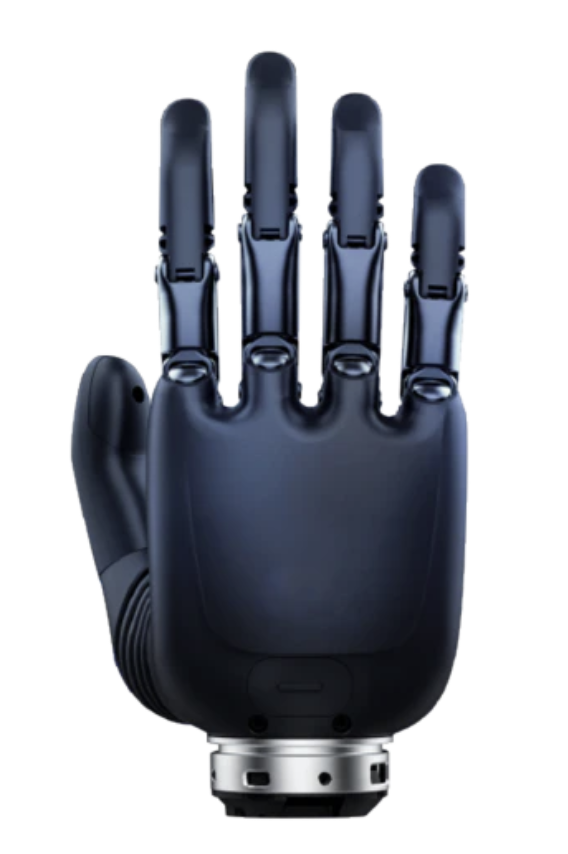
\includegraphics[height=6cm]{figs/chapter2/oceantrix.png}
    \caption{OceanTrix Hand desenvolvida pela  OceanTrix Robotics\cite{oceantrix}.}
    \label{fig:oceantrix}
    
\end{figure}



\subsubsection{Agile Hand}

A \textit{Agile Hand} (Figura \ref{fig:agile}), desenvolvida pela Agile Robots SE, é uma mão robótica antropomórfica com 15 a 16 graus de liberdade, distribuídos por 20 articulações, permitindo movimentos complexos e precisos. Cada dedo é modular e atuado por motores elétricos integrados, capazes de gerar até 10 N de força na ponta dos dedos e velocidades de até 360°/s. A mão incorpora sensores de torque e posição em todas as articulações, permitindo controlo em malha fechada com conformidade ativa. É compatível com manipuladores que seguem a norma ISO 9409-1-50-4-M6 e oferece suporte a C++, Python e ROS, com comunicação a 1 kHz por protocolo proprietário\cite{agile}.

\begin{figure}[H]
    \centering
    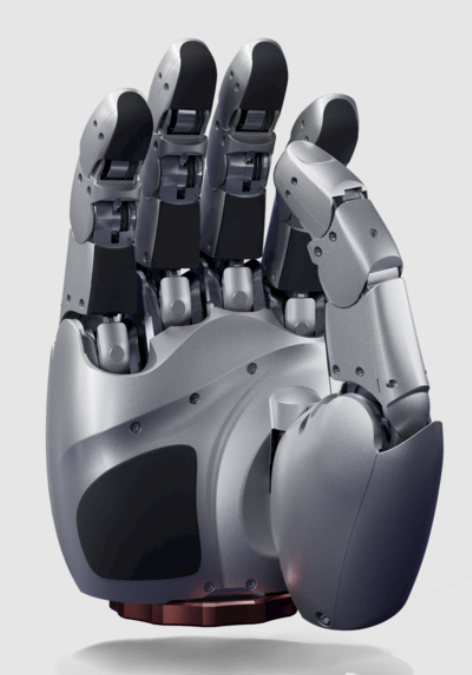
\includegraphics[height=6cm]{figs/chapter2/agile.png}
    \caption{Agile Hand desenvolvida pela Agile Robots SE \cite{agile}.}
    \label{fig:agile}
    
\end{figure}


\subsection{Soluções \textit{open-source}}

As mãos robóticas \textit{open-source} surgem como alternativas acessíveis e personalizáveis às soluções comerciais, especialmente em contextos de investigação e desenvolvimento. Entre as suas principais vantagens destacam-se o baixo custo, a flexibilidade de modificação e a comunidade ativa de utilizadores e desenvolvedores, que facilita a partilha de conhecimento e melhorias contínuas. No entanto, estas soluções apresentam também desvantagens, como a menor robustez mecânica, limitações em precisão e desempenho, e falta de suporte técnico especializado, o que pode representar um desafio em aplicações industriais exigentes.

Para este projeto, a escolha de construir uma mão robótica \textit{open-source} revela-se mais vantajosa, uma vez que será utilizada em contexto de investigação e desenvolvimento, onde a possibilidade de realizar modificações estruturais e funcionais é essencial. Para além disso, a natureza aberta do projeto permite uma maior adaptabilidade aos requisitos específicos da aplicação.


\subsubsection{HRI Hand}

A HRI Hand \cite{Park2020} (Figura \ref{fig:imagem1}) é uma mão robótica antropomórfica \textit{open-source} desenvolvida para atuar como \textit{end-effector} em manipuladores robóticos. Esta mão possui 15 graus de liberdade (sendo apenas 6 juntas ativas),
distribuídos entre os 5 dedos, com cada dedo controlado por um motor linear dedicado, enquanto o polegar utiliza dois motores adicionais para realizar movimentos de abdução e adução. A mão utiliza um mecanismo subatuado baseado num sistema de duas barras articuladas (\textit{four-bar linkage}, ilustrada na figura \ref{fig:imagem2}), permitindo que as articulações \ac{PIP} e \ac{DIP} sejam movidas de forma dependente a partir do motor que controla a articulação \ac{MCP}.

\begin{figure}[h]
    \centering
    \begin{subfigure}[b]{0.45\textwidth} 
        \centering
        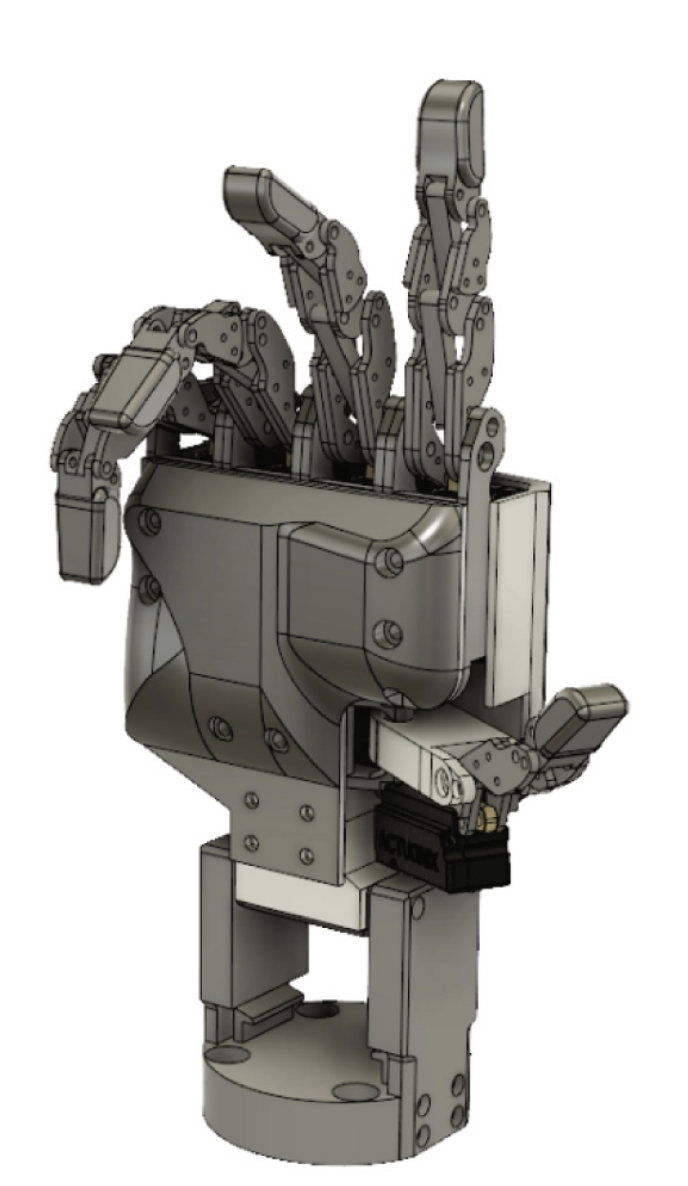
\includegraphics[height=5cm,width=3cm]{figs/chapter2/hri.png}
        \caption{HRI Hand desenvolvida por Park, et al. \cite{Park2020}.}
        \label{fig:imagem1}
    \end{subfigure}
    \hfill
    \begin{subfigure}[b]{0.45\textwidth} 
        \centering
        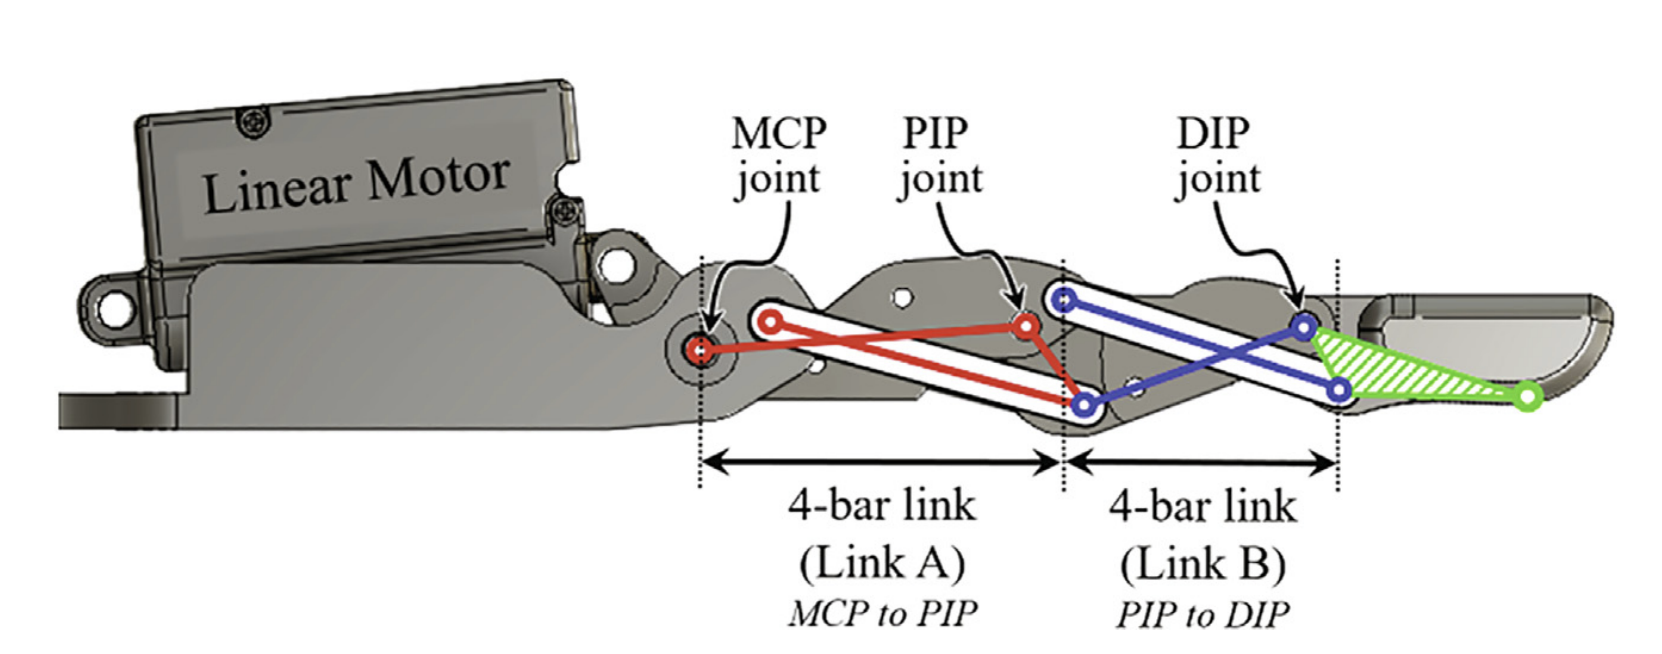
\includegraphics[height=3cm,width=\textwidth]{figs/chapter2/four-bar linkage.png}
        \caption{Sistema de \textit{four-bar linkage} desenvolvida na HRI Hand \cite{Park2020}.}
        \label{fig:imagem2}
    \end{subfigure}
    \caption{Mão HRI e seu mecanismo}
    \label{fig:hri}
\end{figure}

Em termos de compatibilidade de software, a HRI Hand é totalmente integrada com o \ac{ROS} e segue a norma ISO 9409-1-50-4-M6, garantindo compatibilidade com diversos manipuladores robóticos, como o UR3.


\subsubsection{Robot Nano Hand}

A Robot Nano Hand \cite{Nano} (Figura \ref{fig:nano}) é uma mão robótica antropomórfica \textit{open source}, concebida para replicar o tamanho e os movimentos de uma mão humana adulta, oferecendo um total de 11 graus de liberdade. 

A sua estrutura inclui 4 dedos independentes e 1 polegar parcialmente opositor, com cada dedo capaz de realizar movimentos de flexão e laterais, garantindo uma ampla gama de gestos. O sistema de atuação é baseado no uso de tendões, que percorrem os dedos e são controlados por servomotores.

A mão conta também com uma câmara Raspberry Pi V2 integrada na palma, o que a torna adequada para aplicações em visão computacional, incluindo reconhecimento de gestos e análise de objetos. O controlo é gerido por um NVIDIA Jetson Nano Development Kit, um dispositivo robusto que suporta algoritmos de inteligência artificial, como redes neuronais para classificação de imagens e segmentação de objetos.
Embora projetada como uma solução autónoma, com os servos incorporados diretamente na estrutura e um servo adicional que fornece rotação no eixo de inclinação para o conjunto da mão, o design modular da Robot Nano Hand permite adaptações que podem facilitar a sua integração com manipuladores robóticos ou outros sistemas robóticos.

\begin{figure}[H]
    \centering
    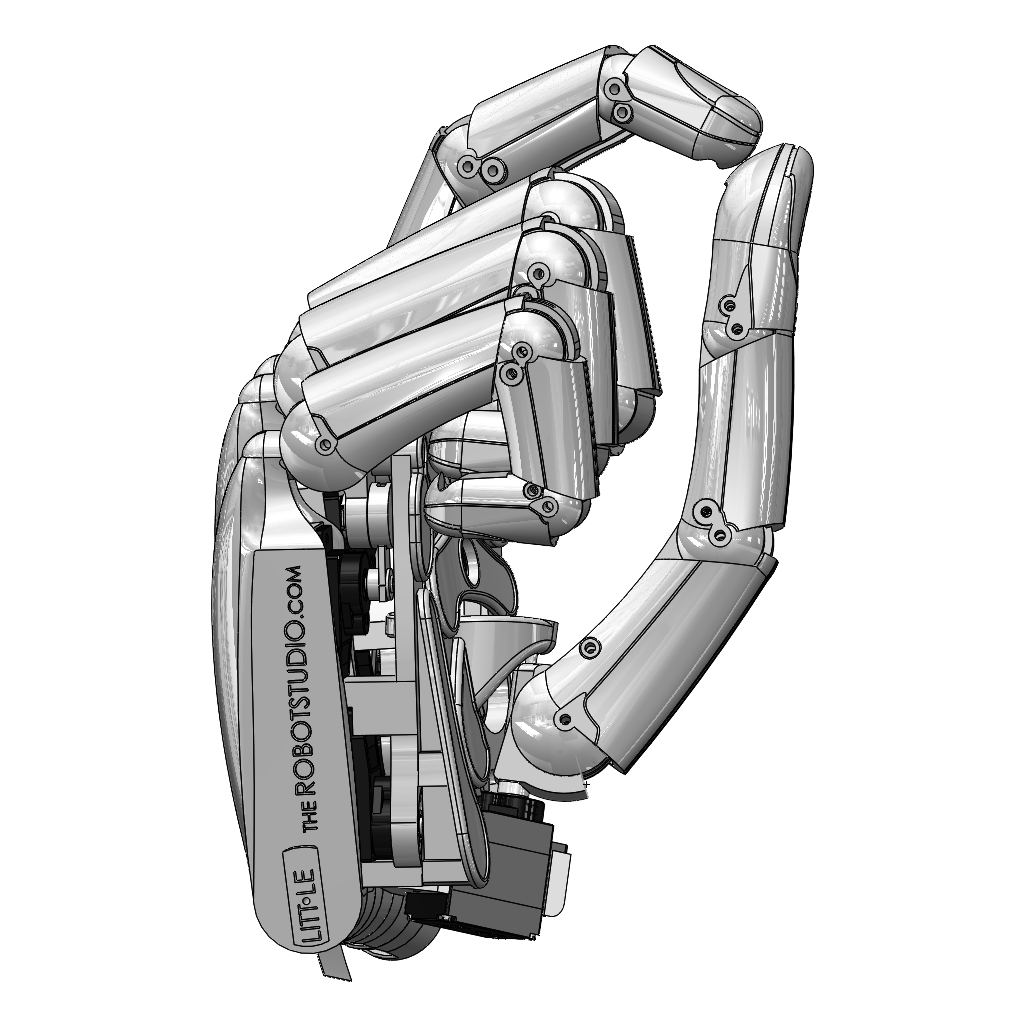
\includegraphics[height=6cm,keepaspectratio]{figs/chapter2/nano.png}
    \caption{Robot Nano Hand desenvolvida por The Robot Studio\cite{Nano}.}
    \label{fig:nano}
    
\end{figure}


\subsubsection{Alaris Hand}

A Alaris Hand \cite{Nurpeissova2021} (Figura \ref{fig:alaris}) é uma mão robótica antropomórfica \textit{open source}, concebida para reproduzir as funcionalidades e movimentos de uma mão humana. 
Este dispositivo apresenta um total de 6 graus de liberdade, permitindo movimentos versáteis dos dedos, que incluem flexão, extensão e manipulação de objetos. 
O sistema de atuação baseia-se em atuadores lineares miniaturizados, acoplados a mecanismos de quatro barras acionados por transmissões de parafuso sem-fim e cremalheira, dispensando o uso de cabos que simulem tendões artificiais. 
Este método garante um controlo eficaz das articulações e proporciona uma força de preensão robusta.
Além disso, a Alaris Hand está equipada com sensores de posição que monitorizam os movimentos articulares em tempo real. 

\begin{figure}[H]
    \centering
    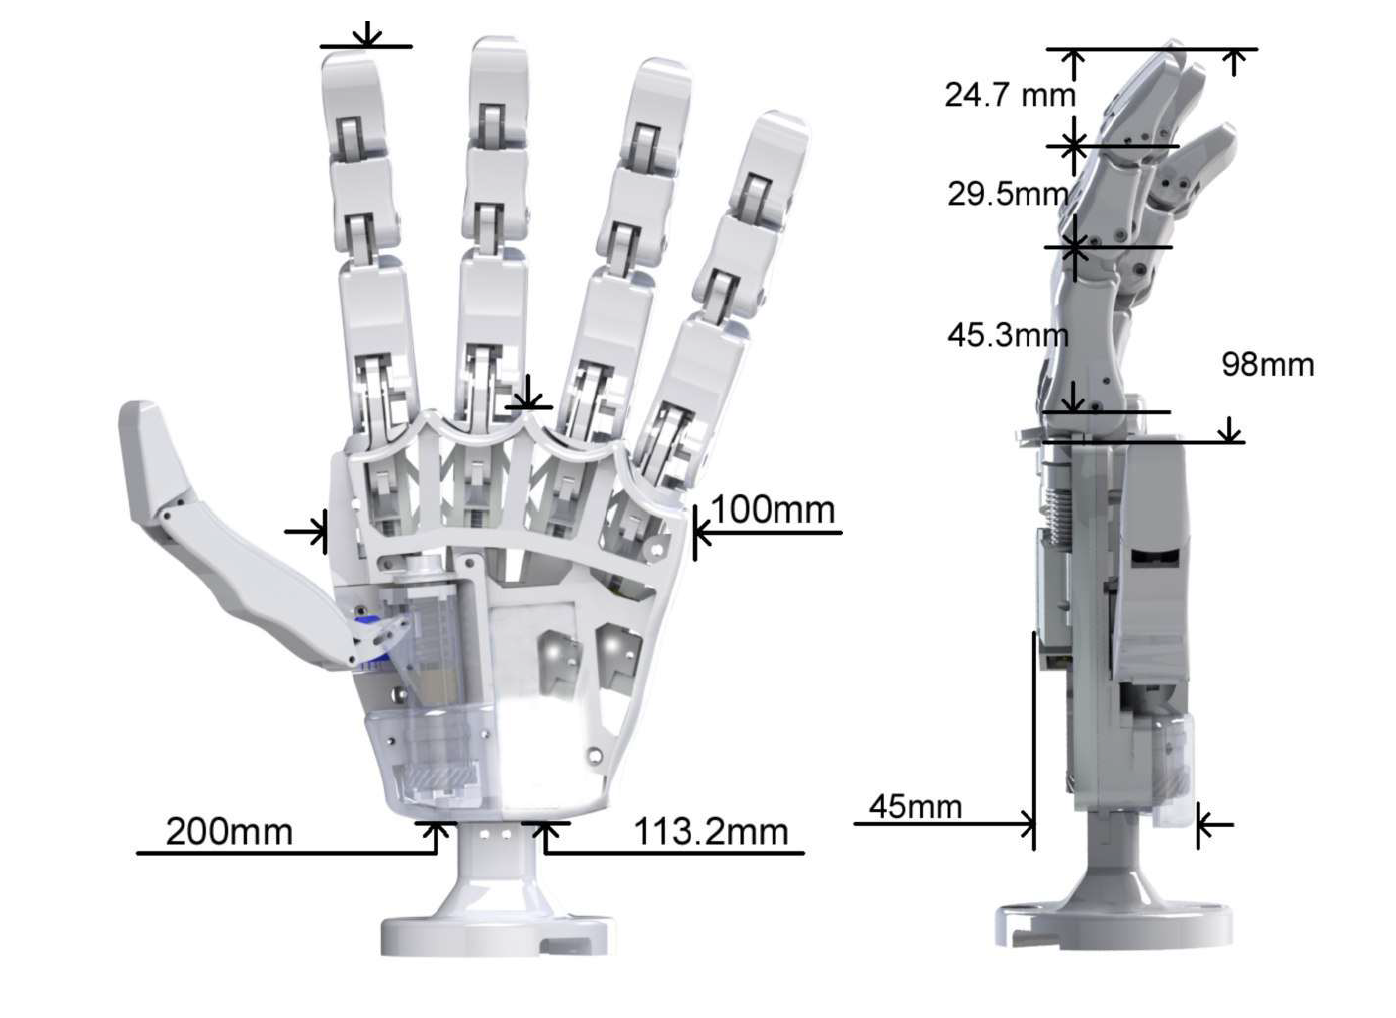
\includegraphics[height=6cm,keepaspectratio]{figs/chapter2/alaris.png}
    \caption{Alaris Hand desenvolvida por Nurpeissova, et al.\cite{Nurpeissova2021}}
    \label{fig:alaris}
    
\end{figure}


\subsubsection{LEAP Hand}

A LEAP Hand \cite{shaw2023leaphand} (Figura \ref{fig:leap_hand})é uma mão robótica antropomórfica de baixo custo, comparado com as soluções comerciais, projetada para aplicações em \textit{machine learning}. 
Esta mão possui 4 dedos e um total de 16 graus de liberdade, com um mecanismo inovador de abdução-adução que mantém todos os graus de liberdade disponíveis em diversas posições das articulações, o que contribui para a sua alta agilidade.
O método de atuação utiliza motores diretos Dynamixel, o que proporciona resistência a torques elevados e aumenta a durabilidade em tarefas de manipulação prolongada.

No que diz respeito aos sensores, a LEAP Hand é capaz de integrar sensores externos para teleoperação ou aprendizagem, mas não possui sensores embutidos nativamente. 
Em termos de software, ela é compatível com diversas plataformas, incluindo \ac{ROS}, Python e C++, além de oferecer um simulador baseado no Isaac Gym e Pybullet, o que permite a realização de experiências de simulação para o mundo real (\textit{sim2real}).

A LEAP Hand é projetada para ser modular e facilmente reparável, utilizando peças impressas em 3D e componentes disponíveis no mercado. A sua compatibilidade com manipuladores robóticos inclui braços como o UR5, o que amplia as suas aplicações em investigação e desenvolvimento.

\begin{figure}[H]
    \centering
    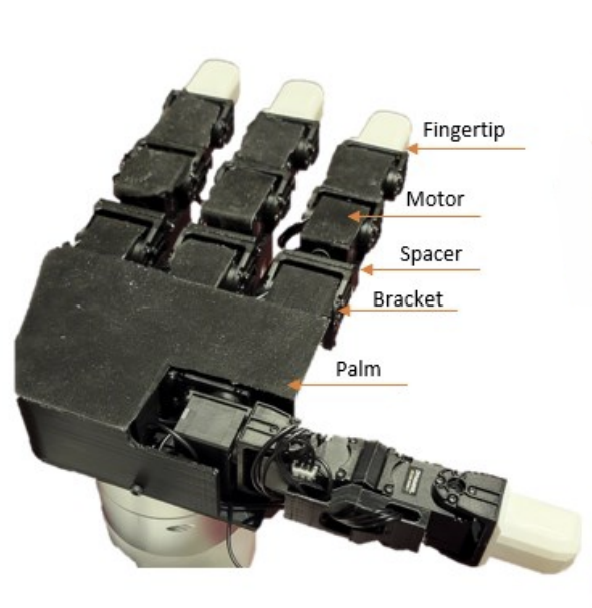
\includegraphics[height=5cm,keepaspectratio]{figs/chapter2/leap_hand.png}
    \caption{Leap Hand desenvolvida por Shaw, et al.\cite{shaw2023leaphand}}
    \label{fig:leap_hand}
    
\end{figure}


\subsection{Seleção da mão a construir}

Após a análise comparativa das diferentes mãos robóticas open-source disponíveis, sumarizada na Tabela~\ref{tab:comparacao_maos}, optou-se pela LEAP Hand~\cite{shaw2023leaphand} como a solução mais adequada para replicação e adaptação no âmbito deste projeto. Esta decisão fundamenta-se principalmente no seu design de construção simples, baseado em servomotores em vez de sistemas de tendões, o que reduz a complexidade mecânica, facilita a montagem e minimiza potenciais pontos de falha.

\begin{table}[H]
    \centering
    \resizebox{\textwidth}{!}{
    \begin{tabular}{l l l l l l}
        \toprule
        \textbf{Modelo} & \textbf{DoF} & \textbf{Atuação} & \textbf{Sensores} & \textbf{Compatibilidade com manipulador} & \textbf{Software} \\
        \midrule
        HRI Hand & 6 & Motores Lineares & Nenhum & UR3 & ROS \\
        Robot Nano Hand & 11 & Tendões & Câmera & Não mencionado & Não mencionado \\     
        Alaris Hand & 6 & Tendões & Posição & Não & Não mencionado \\     
        LEAP Hand & 16 & Servomotores & Posição & UR5 & ROS / Python / C++ / simulação \\
        \bottomrule
    \end{tabular}
    }
    \caption{Comparação entre diferentes mãos robóticas open-source}
    \label{tab:comparacao_maos}
\end{table}

Apesar da sua simplicidade, a LEAP Hand oferece um elevado número de graus de liberdade (16 DoF), superior à maioria das alternativas analisadas, permitindo uma manipulação mais versátil. A presença de sensores de posição integrados garante um controlo eficaz dos movimentos articulares, fator essencial para aplicações em tarefas complexas de manipulação.

Adicionalmente, destaca-se a sua compatibilidade com o sistema ROS, bem como com linguagens de programação como Python e C++, o que proporciona uma plataforma de desenvolvimento acessível e extensível. A possibilidade de integração com manipuladores como o UR5 reforça ainda mais a sua aplicabilidade prática. Por fim, o seu design modular e totalmente imprimível em 3D permite uma manutenção económica e favorece alterações e melhorias iterativas durante o desenvolvimento.



\section{Sensores de Contacto}

A percepção tátil desempenha um papel vital ao permitir que mãos robóticas interajam com o ambiente de forma adaptativa, imitando as capacidades da mão humana.
Esta tecnologia é essencial em áreas como a robótica industrial, onde é necessária uma manipulação precisa, e a aprendizagem por reforço, que se beneficia do \textit{feedback} do mundo real para melhorar o desempenho robótico.

Ao longo dos anos foram propostas diversas tecnologias para sensores táteis, sendo as mais relevantes, no contexto deste trabalho, os sensores baseados em tecnologia magnética, polímeros condutivos e materiais piezoresistivos. Esta secção abordará as principais características e aplicações destas tecnologias em mãos robóticas, destacando as suas vantagens e limitações.

Apesar dos avanços, apenas um número limitado dessas tecnologias tem sido implementado com sucesso em plataformas robóticas reais. Algumas empresas já produzem sensores táteis para aplicações robóticas, como o sensor de ponta de dedo BioTac da SynTouch (ilustrado na figura \ref{fig:biotac})  \cite{Biotac12}. No entanto, estes sensores continuam a apresentar custos elevados e, frequentemente, requerem a integração com outras tecnologias para otimização do desempenho.

\begin{figure}[H]
    \centering
    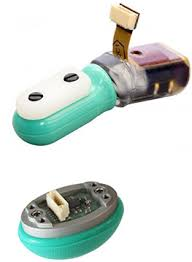
\includegraphics[height=6cm,keepaspectratio]{figs/chapter2/biotac.jpeg}
    \caption{Sensor Biotac desenvolvido pela SynTouch \cite{Biotac12}.}
    \label{fig:biotac}
    
\end{figure}

\subsection{Sensores baseados em Tecnologia Magnética}

Os sensores baseados em tecnologia magnética têm ganho bastante destaque na área da robótica tátil devido à sua elevada precisão, ausência de desgaste e boa durabilidade. Estes sensores destacam-se também por permitirem a deteção de forças sem contacto físico direto com o sensor, o que os torna especialmente interessantes para aplicações em ambientes adversos.

Filmes magnéticos flexíveis, como os apresentados por Jamone, et al. \cite{Jamone2015} (esquema de funcionamento do sensor presente na figura \ref{fig:imagem4}) e  Yan, et al.\cite{Yan2021}, consistem numa camada de elastómero incorporando partículas magnéticas e sensores de efeito Hall colocados abaixo dessa camada. Esta configuração permite medir forças normais e de cisalhamento com elevada sensibilidade, sendo particularmente útil para aplicações em superfícies curvas. No entanto, este tipo de sensor tende a saturar em forças superiores a 4 N, o que limita a sua utilização em tarefas que envolvem forças mais intensas.

\begin{figure}[H]
\centering
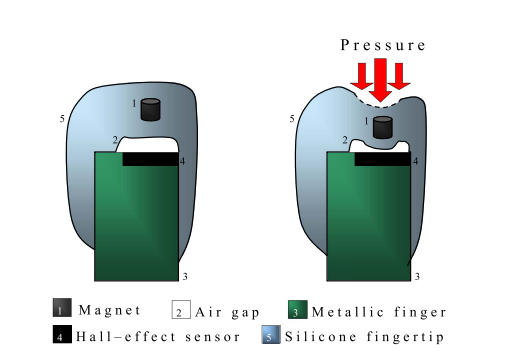
\includegraphics[height=6cm,keepaspectratio]{figs/chapter2/sensor_hall.png}
\caption{Sensor com filme magnético flexível desenvolvido por Jamone, et al. \cite{Jamone2015}.}
\label{fig:imagem4}
\end{figure}



Outra abordagem promissora é o uso de \textit{magneto-elastomer composites}, que combinam materiais elásticos com partículas magnéticas dispersas de forma controlada. Estes sensores, como os utilizados nos trabalhos de Kawasetsu et al. \cite{Kawasetsu2018} (Figura \ref{fig:imagem5}), mostram boa sensibilidade mesmo em contactos rápidos e com elevada aceleração, para além de apresentarem resposta estável a forças contínuas. Contudo, o processo de fabrico pode ser complexo, o que pode implicar maiores custos e limitações em termos de flexibilidade geométrica.

\begin{figure}[H]
\centering
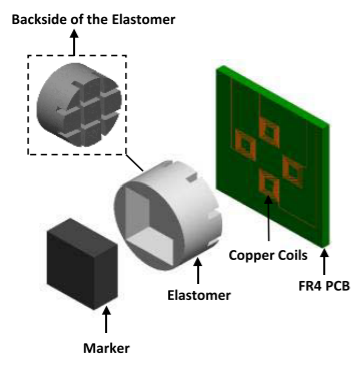
\includegraphics[height=6cm,keepaspectratio]{figs/chapter2/magneto-elastomer.png}
\caption{Composição do sensor desenvolvido por Kawasetsu et al. \cite{Kawasetsu2018}.}
\label{fig:imagem5}
\end{figure}

Os sensores magnetoresistivos representam uma alternativa particularmente robusta, sendo eficazes mesmo em condições adversas como altas temperaturas, humidade ou ambientes com poeiras. O sensor desenvolvido por Alfadhel et al.\cite{Alfadhel2016} utiliza uma estrutura em espiral com materiais magnetoresistivos sensíveis ao campo magnético gerado por uma fonte próxima. Embora a sua robustez seja uma vantagem, estes sensores exigem elevada precisão na montagem e estabilidade dos campos magnéticos externos, o que pode complicar a sua integração em sistemas compactos e móveis \cite{Yang2022}.

\begin{figure}[H]
\centering
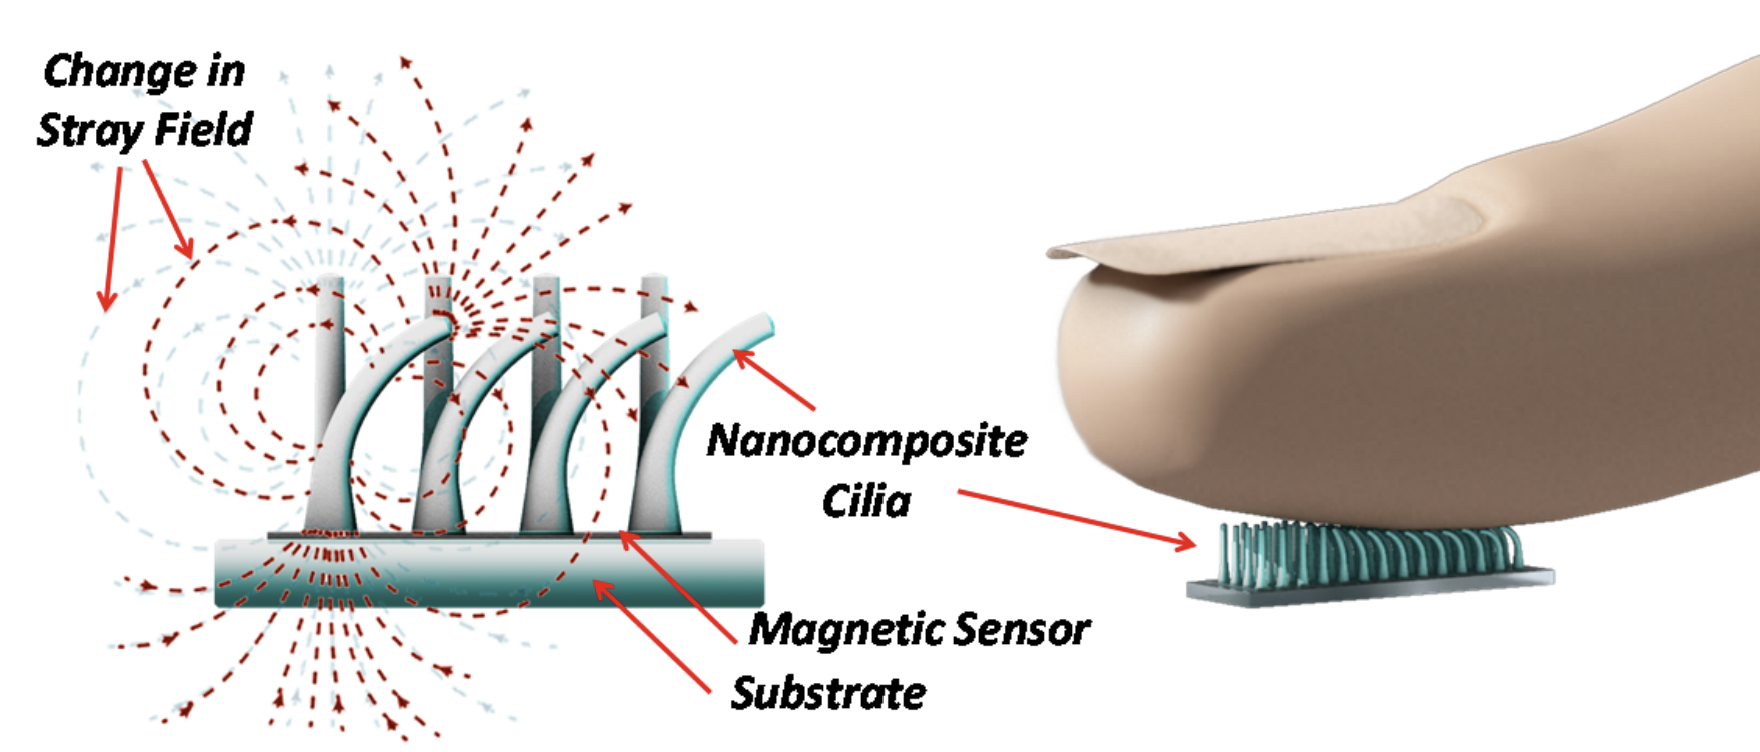
\includegraphics[height=4cm,keepaspectratio]{figs/chapter2/magneto_resistive.png}
\caption{Princípio de operação do sensor baseado em materiais magnetoresistivos \cite{Alfadhel2016}.}
\label{fig:img7}
\end{figure}

Apesar dos desafios, os sensores magnéticos continuam a evoluir e a mostrar grande potencial, sobretudo em aplicações onde a precisão e a resistência a condições ambientais extremas são fundamentais.

\subsection{Sensores baseados em Polímeros Condutivos}

Os sensores baseados em polímeros condutivos têm-se destacado como soluções promissoras para aplicações táteis em sistemas robóticos, sobretudo pela sua leveza, flexibilidade e facilidade de adaptação a superfícies irregulares. Estes dispositivos exploram a variação das propriedades elétricas de materiais condutivos em resposta a deformações mecânicas, permitindo a detecção eficiente de toque e pressão.

Entre as principais abordagens, destacam-se os sensores piezoresistivos, que se baseiam na alteração da resistência elétrica com a aplicação de pressão. São dispositivos de baixo custo e integração simples, adequados para superfícies complexas, como demonstrado em \cite{Canavese2014, Stassi2014}. Contudo, apresentam limitações em termos de precisão, resposta não linear e durabilidade.

Os sensores piezoelétricos, por sua vez, utilizam materiais como o \ac{PVDF}, capazes de gerar sinais elétricos sob estímulos dinâmicos. São valorizados pela elevada sensibilidade, leveza e flexibilidade \cite{Yin2023, Seminara2012}, sendo eficazes na deteção de vibrações e forças variáveis. No entanto, não são apropriados para medições de forças estáticas e requerem circuitos de condicionamento de sinal mais complexos.

Adicionalmente, os sensores triboelétricos operam com base na eletrificação por contato, sendo capazes de gerar sinais elétricos de forma autossuficiente, sem necessidade de alimentação externa. Trabalhos recentes \cite{Zhong2023, Tao2022} demonstram o seu bom desempenho em ambientes adversos. Ainda assim, enfrentam desafios associados à fragilidade mecânica, complexidade de fabrico e sensibilidade a fatores ambientais.

% \begin{figure}[H]
%     \centering
%     \begin{subfigure}[b]{0.45\textwidth} 
%         \centering
%         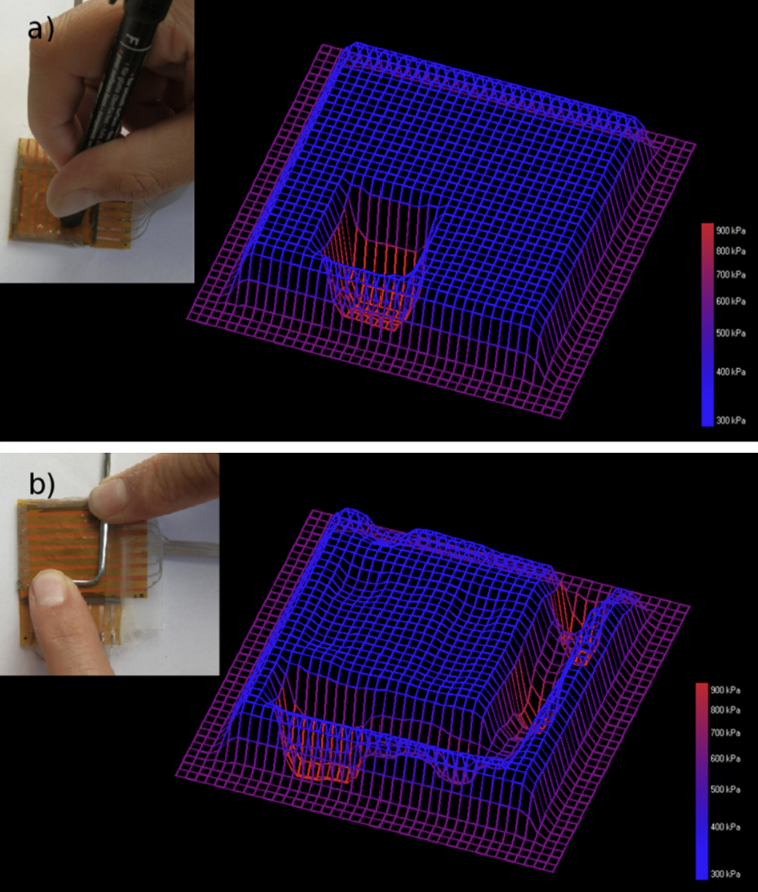
\includegraphics[height=4cm,keepaspectratio]{figs/chapter2/testes.png}
%         \caption{Testes realizados com o sensor desenvolvido em \cite{Canavese2014}.}
%         \label{fig:imagem7}
%     \end{subfigure}
%     \hfill
%     \begin{subfigure}[b]{0.45\textwidth} 
%         \centering
%         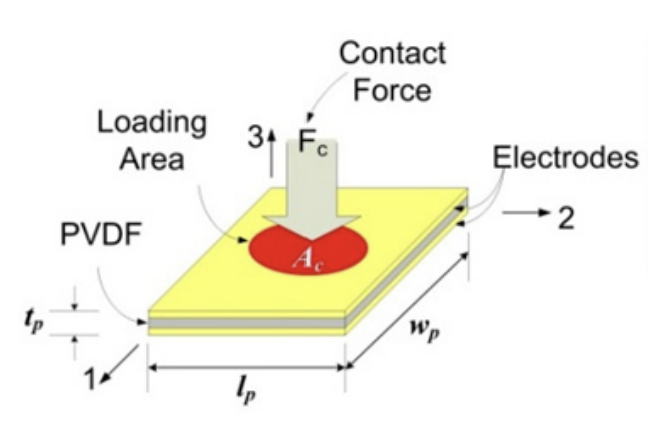
\includegraphics[height=3cm,keepaspectratio]{figs/chapter2/pvdf.png}
%         \caption{Estrutura de um sensor baseado em \ac{PVDF}.}
%         \label{fig:imagem6}
%     \end{subfigure}
%     \caption{Sensores baseados em materiais piezoresistivos}
%     \label{fig:img8}
% \end{figure}


\subsection{Sensores baseados em Materiais Piezoresistivos}

Os sensores baseados em materiais piezoresistivos têm sido amplamente utilizados em aplicações de sensoriamento tátil, especialmente no domínio da robótica, devido à sua elevada sensibilidade à aplicação de forças e pressões. O seu funcionamento baseia-se na variação da resistência eléctrica resultante de deformações mecânicas, permitindo medições precisas e localizadas.

Um exemplo representativo desta tecnologia são os sensores de resistência sensível à força (\acp{FSR}), que combinam um design compacto e robusto com uma elevada adaptabilidade a superfícies curvas e complexas, como as encontradas em mãos robóticas \cite{Ke2019, Lu2023}. Estas características tornam-nos particularmente adequados para sistemas de deteção tátil de baixo custo e fácil integração.

Entre as principais vantagens dos sensores piezoresistivos destacam-se o custo reduzido de produção, a leveza, a flexibilidade e a possibilidade de personalização da sensibilidade em função dos requisitos da aplicação \cite{Stassi2014}. Para além disso, a simplicidade do seu princípio de funcionamento facilita a integração com circuitos eletrónicos de leitura e controlo.

No entanto, estes sensores apresentam também algumas limitações. A sua precisão é, por vezes, inferior à de outras tecnologias sensoriais, e a resposta não linear pode dificultar a calibração. Adicionalmente, a durabilidade e a estabilidade da resposta ao longo do tempo podem ser comprometidas, especialmente em aplicações sujeitas a esforços repetidos ou prolongados \cite{Ke2019}.

% \begin{figure}[H]
%     \centering
%     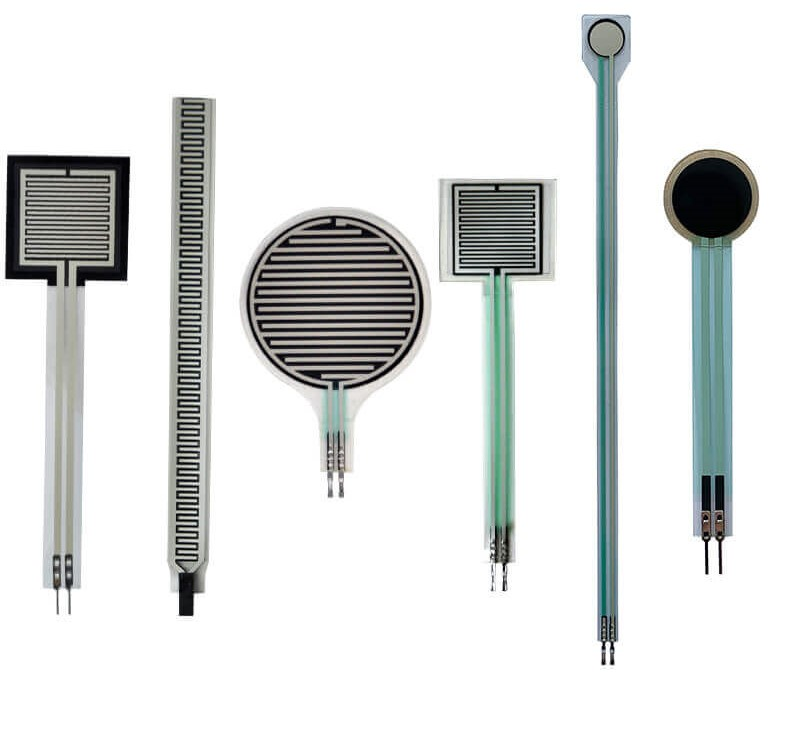
\includegraphics[height=4cm]{figs/chapter2/fsr.jpg}
%     \caption{Sensores \ac{FSR} desenvolvidos pela Interlink.}
%     \label{fig:img9}
    
% \end{figure}


\subsection{Escolha dos sensores a incorporar no projeto}

A seleção dos sensores táteis para o presente projeto foi fundamentada numa análise comparativa entre as diferentes tecnologias disponíveis, com base em critérios como princípio de funcionamento, vantagens técnicas e limitações práticas. A Tabela~\ref{tab:comparacao_sensores} apresenta uma síntese dos principais tipos de sensores considerados.

\begin{table}[H]
    \centering
    \resizebox{\textwidth}{!}{%
    \begin{tabular}{|l|p{5cm}|p{5cm}|p{5cm}|}
        \hline
        \textbf{Tipo de Sensor} & \textbf{Princípio de Funcionamento} & \textbf{Vantagens} & \textbf{Desvantagens} \\
        \hline
        \textbf{Magnético} & Deteta variações em campos magnéticos sem contacto físico direto & Elevada precisão, ausência de desgaste mecânico, boa durabilidade & Custo mais elevado, suscetibilidade a interferência magnética, maior complexidade \\
        \hline
        \textbf{Polímero Condutivo} & Condutividade elétrica varia com a deformação mecânica do material & Elevada sensibilidade, flexibilidade, leveza & Menor durabilidade, sensibilidade a fatores ambientais, resposta lenta \\
        \hline
        \textbf{Piezoresistivo (FSR)} & Resistência elétrica diminui com o aumento da pressão aplicada & Baixo custo, fácil integração, formato compacto e flexível & Resposta não linear, menor precisão, vida útil limitada \\
        \hline
    \end{tabular}%
    }
    \caption{Comparação entre diferentes tipos de sensores táteis}
    \label{tab:comparacao_sensores}
\end{table}

Com base na análise comparativa realizada, os sensores piezoresistivos do tipo \ac{FSR} foram selecionados como a solução mais adequada para o projeto em desenvolvimento. Esta decisão fundamenta-se num conjunto de fatores que favorecem a sua aplicação em contextos de robótica tátil, nomeadamente em mãos robóticas.

Em primeiro lugar, destaca-se a sua estrutura fina, leve e flexível, que permite uma integração eficiente em superfícies curvas, como as pontas dos dedos e a palma da mão robótica. Para além disso, os \acp{FSR} oferecem um equilíbrio vantajoso entre desempenho e acessibilidade económica.

Adicionalmente, o seu design compacto e a simplicidade de integração com os sistemas eletrónicos permitem reduzir significativamente a complexidade de implementação, fator particularmente relevante em projetos com restrições de espaço físico, como é o caso da LEAP Hand \cite{shaw2023leaphand}.



\section{Conclusão}

Ao longo deste capítulo foram analisadas várias opções tecnológicas com vista à definição da arquitetura sensorial do projeto. Numa primeira fase, avaliou-se um conjunto de mãos robóticas antropomórficas, tanto comerciais como open-source, com o objetivo de selecionar uma solução adequada aos requisitos de integração tátil. Desta análise resultou a escolha da LEAP Hand\cite{shaw2023leaphand}, cuja estrutura modular, dimensões compactas e compatibilidade com sensores externos a tornam particularmente apropriada para o presente projeto.

De seguida, procedeu-se ao estudo comparativo de diferentes tecnologias sensoriais, nomeadamente sensores baseados em princípios magnéticos, polímeros condutivos e materiais piezoresistivos. A avaliação teve em consideração fatores como sensibilidade, facilidade de integração e viabilidade económica.

Com base nesta análise, foram selecionados sensores piezoresistivos do tipo \ac{FSR}, devido ao seu formato compacto, baixo custo, facilidade de aplicação em superfícies curvas e capacidade de resposta adequada aos requisitos de deteção tátil em mãos robóticas.

Em suma, as decisões tomadas relativamente à mão robótica e à tecnologia sensorial asseguram uma base sólida para o desenvolvimento do sistema de perceção tátil, alinhando-se com os objetivos técnicos e funcionais definidos para o projeto.


\chapter{Ferramentas de suporte}
\label{chapter:suporte}

\section{Introdução}

A adoção de uma mão robótica \textit{open-source} apresenta diversas vantagens, entre as quais se destacam a disponibilização de código de apoio e a existência de decisões previamente fundamentadas relativamente à seleção de componentes mecânicos e eletrónicos. Estas características permitem reduzir significativamente o tempo necessário para o desenvolvimento de um sistema funcional, evitando o esforço associado ao desenho e especificação de soluções desde a parte inicial do projeto. 

Neste capítulo, descrevem-se os principais elementos já existentes e utilizados como base no presente trabalho, com particular destaque na LEAP Hand, desenvolvida por Shaw, et al. \cite{shaw2023leaphand}. Serão abordadas as escolhas efetuadas por estes autores ao nível dos motores, do controlador de motores, da fonte de alimentação e das ferramentas de software disponibilizadas, que serviram de ponto de partida para o desenvolvimento realizado neste projeto.

\section{Hardware}

\subsection{Motores Dynamixel}

No desenvolvimento da LEAP Hand, Shaw, et al. \cite{shaw2023leaphand} optaram por utilizar os motores Dynamixel XC330-M288-T, amplamente utilizados em aplicações robóticas devido à sua fiabilidade, eficiência energética e dimensões compactas. Estes atuadores oferecem controlo detalhado sobre posição, velocidade e corrente, permitindo gerar movimentos suaves, reproduzíveis e bem definidos — uma característica fundamental em sistemas de manipulação, como mãos robóticas antropomórficas. 

Os motores Dynamixel XC330-M288-T (Figura \ref{fig:motor}) operam a 5V e apresentam uma corrente nominal de 1.8A, o que os torna compatíveis com fontes de alimentação de baixa potência, mantendo um desempenho consistente. Adicionalmente, a comunicação digital via protocolo TTL permite a ligação e controlo eficiente de múltiplos motores em rede, facilitando a sua integração com microcontroladores e promovendo uma arquitetura modular e escalável.

\begin{figure}[H]
    \centering
    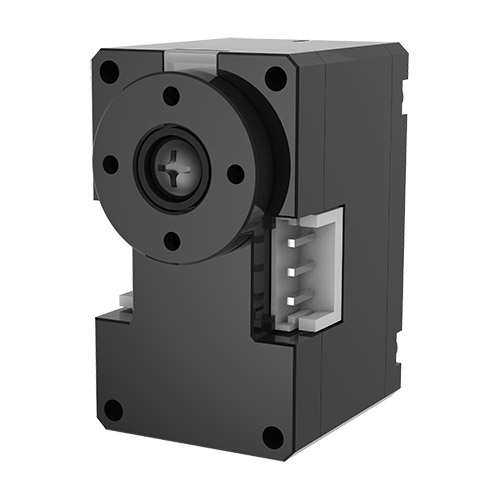
\includegraphics[height=6cm]{figs/chapter3/motor.jpg}
    \caption{Motor Dynamixel XC330-M288-T utilizado na construção da LEAP Hand\cite{shaw2023leaphand} }
    \label{fig:motor}
    
\end{figure}

O controlo destes motores pode ser realizado por diferentes meios, nomeadamente através da ferramenta gráfica Dynamixel Wizard 2.0, útil para configuração e diagnóstico, e da biblioteca Dynamixel SDK, que permite o controlo programático e a integração com sistemas desenvolvidos em diversas linguagens de programação. Estas opções tornam o sistema versátil e facilmente adaptável a diferentes contextos de desenvolvimento, incluindo ambientes compatíveis com \ac{ROS}.

Os motores Dynamixel armazenam e gerem os seus parâmetros internos através de uma tabela de controlo de memória, onde cada parâmetro — como posição, velocidade, corrente ou temperatura — está associado a um endereço específico. Essa tabela encontra-se dividida em duas secções principais: a \textbf{EEPROM}, que contém parâmetros permanentes (como o ID do motor, taxa de transmissão, limites de corrente ou posição) e só pode ser modificada após a reinicialização do motor; e a \textbf{RAM}, onde se encontram os parâmetros dinâmicos, como a posição atual, velocidade, temperatura e estado do motor, permitindo atualizações em tempo real durante a operação. Esta estrutura torna o controlo dos motores altamente flexível e eficiente, uma vez que permite o acesso direto e segmentado aos dados necessários para a gestão do comportamento do sistema robótico.

\subsection{Controlador e Fonte de Alimentação}

Para além da seleção dos motores, a escolha do controlador de comunicação e da fonte de alimentação tem um impacto significativo no desempenho e na fiabilidade do sistema. No que respeita à interface de comunicação com os motores, os autores da LEAP Hand \cite{shaw2023leaphand} optaram por utilizar o \textbf{Dynamixel U2D2} (Figura \ref{fig:u2d2}), um conversor USB para TTL \textit{half-duplex}.  Este dispositivo permite estabelecer comunicação entre um computador e múltiplos motores Dynamixel através de uma única porta serial, utilizando um barramento em cadeia (\textit{daisy chain}). Este método de ligação, possível graças à arquitetura \textit{half-duplex} dos motores, permite que vários atuadores sejam ligados em série, reduzindo significativamente a complexidade do sistema e facilitando a sincronização entre motores. O U2D2 suporta taxas de transmissão elevadas (até 4,5 Mbps), possui um conector JST de 3 pinos para comunicação TTL, e inclui um terminal de alimentação auxiliar (VDD), permitindo a alimentação dos motores a partir de uma fonte externa apropriada. 

Relativamente à fonte de alimentação, foi necessário considerar que cada motor Dynamixel XC330-M288-T pode atingir um consumo máximo de 1.8A em condições de carga. Tendo em conta a utilização de 16 motores, a corrente total exigida pode atingir os 28.8A. Assim, foi selecionada uma fonte de alimentação industrial (Figura \ref{fig:fonte}) com saída estabilizada de 5V — a mesma tensão nominal dos motores — e capacidade de fornecimento de até 30A, assegurando uma margem de segurança adequada para o funcionamento simultâneo de todos os atuadores.

\begin{figure}[H]
    \centering
    \begin{minipage}[b]{0.45\textwidth}
        \centering
        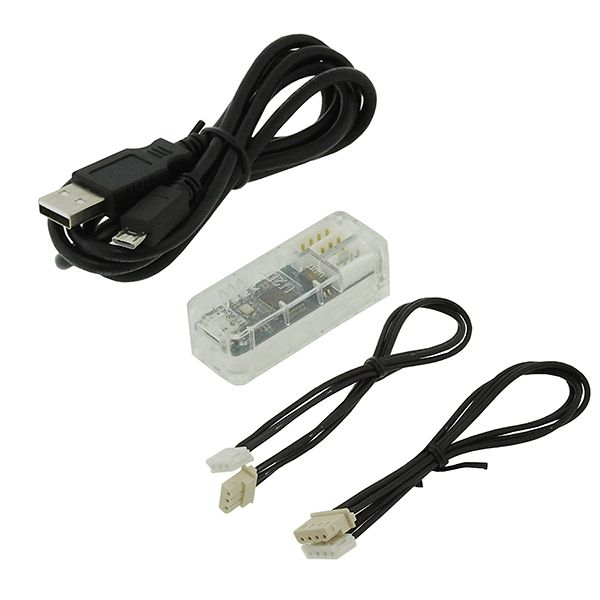
\includegraphics[width=\textwidth]{figs/chapter3/u2d2.jpg}
        \caption{Controlador Dynamixel U2D2 utilizado para controlar os motores do projeto}
        \label{fig:u2d2}
    \end{minipage}
    \hfill
    \begin{minipage}[b]{0.45\textwidth}
        \centering
        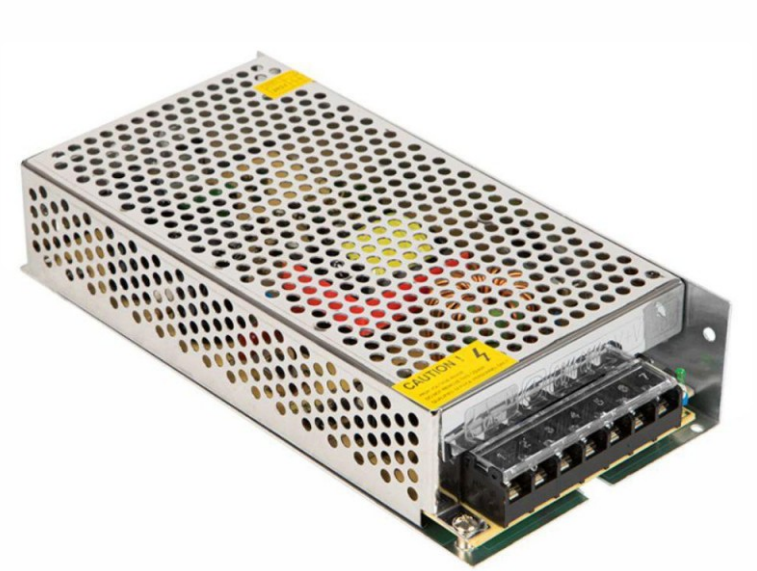
\includegraphics[width=\textwidth]{figs/chapter3/fonte.png}
        \caption{Fonte de Alimentação industrial com saída a 5V e capacidade de 30A utilizada neste projeto}
        \label{fig:fonte}
    \end{minipage}
\end{figure}


\section{Software}

\subsection{Dynamixel Wizard 2.0}

A Dynamixel disponibiliza diversas ferramentas para configuração, monitorização e controlo dos seus motores, entre as quais se destaca o Dynamixel Wizard 2.0, uma interface gráfica intuitiva (Figura \ref{fig:dynamixel_wizard}) que permite ao utilizador interagir diretamente com cada motor. Antes de iniciar o controlo coordenado de um sistema com múltiplos atuadores, é essencial garantir que cada motor possui um identificador único. Por defeito, todos os motores Dynamixel são fornecidos com o mesmo identificador (ID = 1), o que inviabiliza a sua utilização simultânea num mesmo barramento de comunicação. Assim, uma das primeiras tarefas consiste na atribuição de um ID exclusivo a cada motor, procedimento que pode ser facilmente realizado através do Dynamixel Wizard 2.0, modificando o parâmetro correspondente no firmware do atuador.


\begin{figure}[H]
    \centering
    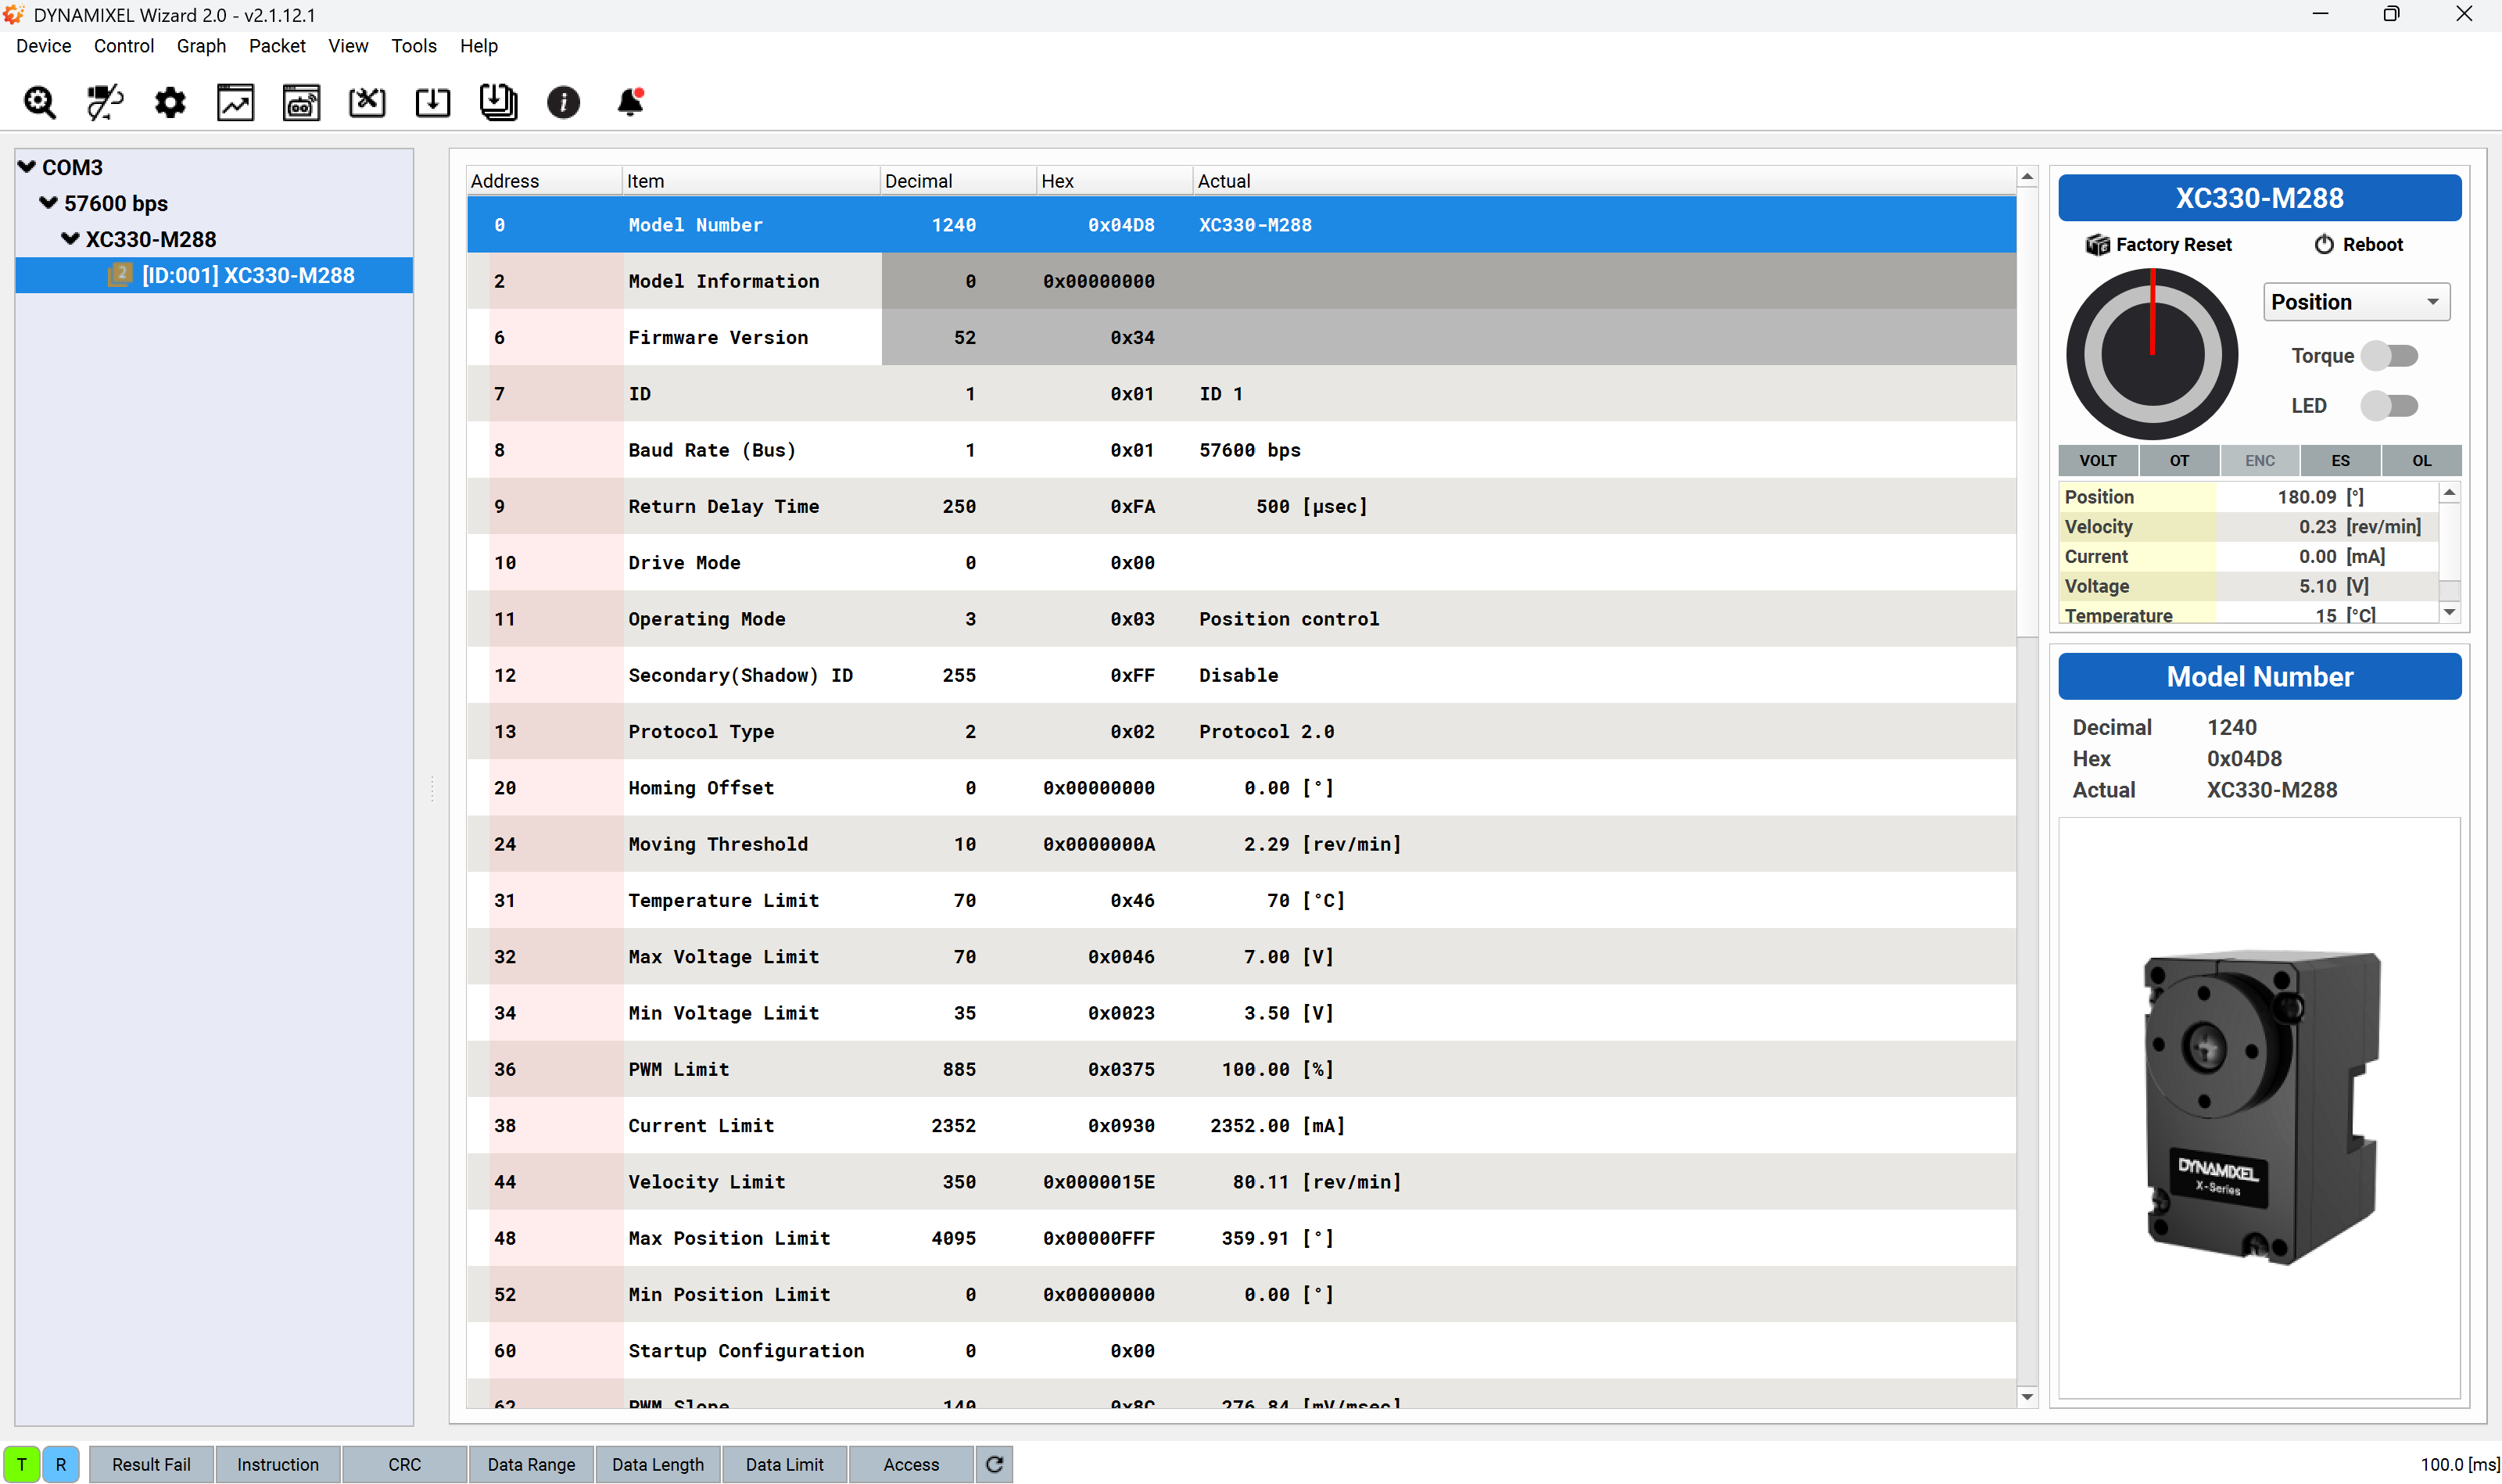
\includegraphics[height=8cm]{figs/chapter3/dynamixel_wizard.png}
    \caption{Interface Gráfica da ferramenta Dynamixel Wizard 2.0 utilizada para alterar o ID de cada motor}
    \label{fig:dynamixel_wizard}
    
\end{figure}


Para além da atribuição de IDs individuais, esta ferramenta permite ainda a definição de grupos de motores com IDs secundários, úteis para cenários em que se pretende acionar vários motores em simultâneo e de forma idêntica. No entanto, esta funcionalidade não será explorada neste projeto, dado que o controlo será efetuado de forma independente para cada atuador.

Adicionalmente, o Dynamixel Wizard 2.0 oferece funcionalidades de diagnóstico e monitorização em tempo real, possibilitando a visualização de parâmetros como a posição atual, velocidade, corrente consumida, entre outros. Esta capacidade é particularmente útil durante as fases de teste, permitindo validar o comportamento dos motores e detetar eventuais anomalias no sistema.

\subsection{Biblioteca Dynamixel SDK}

O Dynamixel SDK é uma biblioteca de software multiplataforma que permite a comunicação e o controlo eficiente dos motores Dynamixel em diversas linguagens de programação, tais como Python, C, C++ e Java. Concebido para proporcionar uma interface unificada e de alto nível, o SDK abstrai as complexidades da comunicação serial, simplificando as operações de leitura e escrita de dados nos motores.

Esta biblioteca suporta os principais protocolos de comunicação Dynamixel, incluindo o Protocolo 2.0, utilizado no presente projeto para os motores XC330-M288-T, o que assegura compatibilidade com as funcionalidades mais recentes dos atuadores, como o controlo de corrente, modos operacionais configuráveis e diagnósticos internos. Através do SDK, é possível configurar parâmetros como posição, velocidade, corrente máxima, limites de movimento e modo de operação, permitindo adaptar o comportamento dos motores às exigências específicas de cada aplicação.

\subsection{ROS2}

O \ac{ROS} é uma \textit{framework} amplamente utilizada no desenvolvimento de sistemas robóticos, proporcionando um ambiente modular que facilita o desenvolvimento, gestão e interligação de múltiplos nós que executam tarefas específicas em paralelo. Esta arquitetura distribuída permite uma organização estruturada do código, promovendo a escalabilidade e a reutilização de componentes, o que é particularmente vantajoso em projetos complexos, como o desenvolvimento de mãos robóticas antropomórficas.

No âmbito da LEAP Hand, Shaw et al. \cite{shaw2023leaphand} disponibilizaram documentação e exemplos compatíveis com Python, ROS 1 e ROS 2, conferindo flexibilidade na escolha da infraestrutura de desenvolvimento. Neste projeto, optou-se pela utilização do ROS 2, em detrimento do ROS 1, com base nas vantagens técnicas e estruturais que a nova versão oferece.

Entre os principais fatores que justificam esta escolha destacam-se a utilização do \textit{middleware \ac{DDS}}, que melhora substancialmente a comunicação entre nós, tornando-a mais eficiente e robusta — um requisito fundamental em sistemas com múltiplos atuadores e sensores a operar em tempo real. Para além disso, o ROS 2 elimina a necessidade de um nó central como o \textit{rosmaster}, permitindo uma arquitetura verdadeiramente distribuída e mais resiliente a falhas. Esta mudança traduz-se numa maior robustez e flexibilidade na gestão da rede de nós, especialmente em contextos com comunicações complexas ou heterogéneas.

Outro fator relevante é o fim gradual do suporte ao ROS 1, cuja manutenção oficial está em fase de descontinuação, sendo que muitas das novas bibliotecas e ferramentas estão a ser exclusivamente desenvolvidas para o ROS 2. A adoção do ROS 2 assegura, portanto, maior longevidade, compatibilidade com futuras atualizações e acesso a funcionalidades mais recentes da comunidade de robótica.

Por fim, o suporte nativo a sistemas real-time, a maior portabilidade entre plataformas e o foco na segurança e escalabilidade reforçam a decisão de utilizar o ROS 2 neste projeto. Esta escolha visa garantir um desenvolvimento mais moderno e sustentável, mantendo a compatibilidade com sistemas robóticos avançados e preparados para integração em ambientes distribuídos.

\subsection{Documentação da LEAP Hand}

Os autores da LEAP Hand \cite{shaw2023leaphand} disponibilizam documentação detalhada e exemplos de código para facilitar a reprodução e o desenvolvimento com base na sua plataforma. Embora essa documentação suporte a utilização em Python, ROS 1 e ROS 2, o código fornecido foi desenvolvido com um foco específico: a execução de políticas previamente treinadas em simulação (utilizando o simulador incluído no projeto) e a realização de movimentos predefinidos da mão robótica.

No entanto, esta abordagem não contempla a possibilidade de controlo direto e individualizado dos motores, nem permite uma personalização completa do comportamento da mão, o que limita a sua aplicabilidade em contextos que exigem maior flexibilidade no desenvolvimento de novos controladores ou algoritmos de manipulação.

Tendo em conta estas limitações, e considerando os objetivos deste projeto, optou-se por não utilizar diretamente o código disponibilizado pelos autores da LEAP Hand, desenvolvendo-se, em alternativa, uma nova infraestrutura de controlo que permite acesso completo e individualizado a cada motor, facilitando o desenvolvimento de estratégias de controlo personalizadas e adaptadas às necessidades específicas deste trabalho.





\section{Conclusão}

Ao longo deste capítulo, foram apresentadas as principais ferramentas de suporte utilizadas no desenvolvimento do projeto, com especial destaque nos componentes de hardware e software que viabilizam a implementação da mão robótica. 

Inicialmente, identificaram-se os motores Dynamixel XC330-M288-T e o controlador U2D2 como soluções adequadas para assegurar movimentos compatíveis com a estrutura da LEAP Hand. A fonte de alimentação foi selecionada com base nas exigências energéticas do sistema, garantindo estabilidade e segurança durante a operação.

Paralelamente, foram descritas as ferramentas de software de apoio à configuração e controlo dos motores, nomeadamente o Dynamixel Wizard 2.0 e a biblioteca Dynamixel SDK, bem como o ambiente de desenvolvimento baseado em ROS 2, que oferece escalabilidade e integração com outros módulos do sistema.

Adicionalmente, a documentação da LEAP Hand foi analisada como referência complementar, optando-se por não utilizar diretamente o código disponibilizado de forma a permitir o controlo individualizado de cada motor.

Em suma, a seleção e integração das ferramentas de suporte descritas neste capítulo estabeleceram uma infraestrutura adaptada às necessidades do sistema, contribuindo para a robustez, modularidade e evolução futura do desenvolvimento da mão robótica.


\chapter{Projeto e Implementação da Solução}
\label{chapter:solução}

\section{Introdução}

Este capítulo apresenta o processo de desenvolvimento da solução proposta, desde a construção física da mão robótica até à implementação do sistema sensorial.  Inicia-se com a apresentação das etapas associadas ao fabrico e montagem da estrutura da mão robótica, seguindo-se a configuração dos motores e o desenvolvimento da lógica de controlo, desde o acionamento de motores individuais até ao controlo coordenado da mão completa.

É igualmente descrita a arquitetura de software desenvolvida, com especial destaque para as funcionalidades avançadas implementadas, como o ajuste dinâmico de corrente durante o contacto com objetos, a definição de velocidades relativas entre dedos e falanges, e a introdução de atrasos temporais entre movimentos.

Adicionalmente, aborda-se a implementação do sistema sensorial de deteção de contacto, incluindo a seleção do microcontrolador, o desenvolvimento físico da unidade de aquisição e os testes realizados com diferentes sensores. 

\section{Desenvolvimento da Mão Robótica}



\subsection{Fabrico e Montagem da estrutura}

A construção da estrutura da mão robótica seguiu integralmente as indicações fornecidas na documentação da LEAP Hand, a qual disponibiliza de forma aberta e acessível todos os ficheiros CAD necessários, bem como instruções detalhadas de montagem. Esta abordagem permitiu realizar uma primeira montagem da estrutura de forma fiel ao projeto original, facilitando a replicação inicial da arquitetura mecânica.

As peças foram produzidas por impressão 3D com recurso a uma Creality K1, uma impressora de alto desempenho que assegura uma boa qualidade dimensional e tempos de fabrico reduzidos. Para a estrutura principal foi utilizado o filamento Hyper PLA da Creality, selecionado pela sua rigidez e facilidade de impressão. Já para as pontas dos dedos, onde se pretende maior flexibilidade e capacidade de aderência ao contacto com objetos, foi utilizado o Python Flex TPU da FormFutura.

A construção dos dedos revelou-se a fase mais demorada do processo de montagem, devido ao elevado número de componentes envolvidos e à complexidade dos passos necessários. Todos os dedos seguem a mesma configuração estrutural, com exceção do polegar, que apresenta um desenho distinto adaptado à sua função anatómica e posição na mão.

Na Figura~\ref{fig:polegar} é apresentado o polegar já montado, enquanto na Figura~\ref{fig:dedo} observa-se um dos restantes dedos, com estrutura idêntica entre si. A montagem de cada dedo envolveu operações detalhadas e sequenciais que exigiram precisão e atenção redobrada, especialmente na organização dos cabos e no alinhamento das juntas móveis.

\begin{figure}[H]
    \centering
    \begin{minipage}[b]{0.45\textwidth}
        \centering
        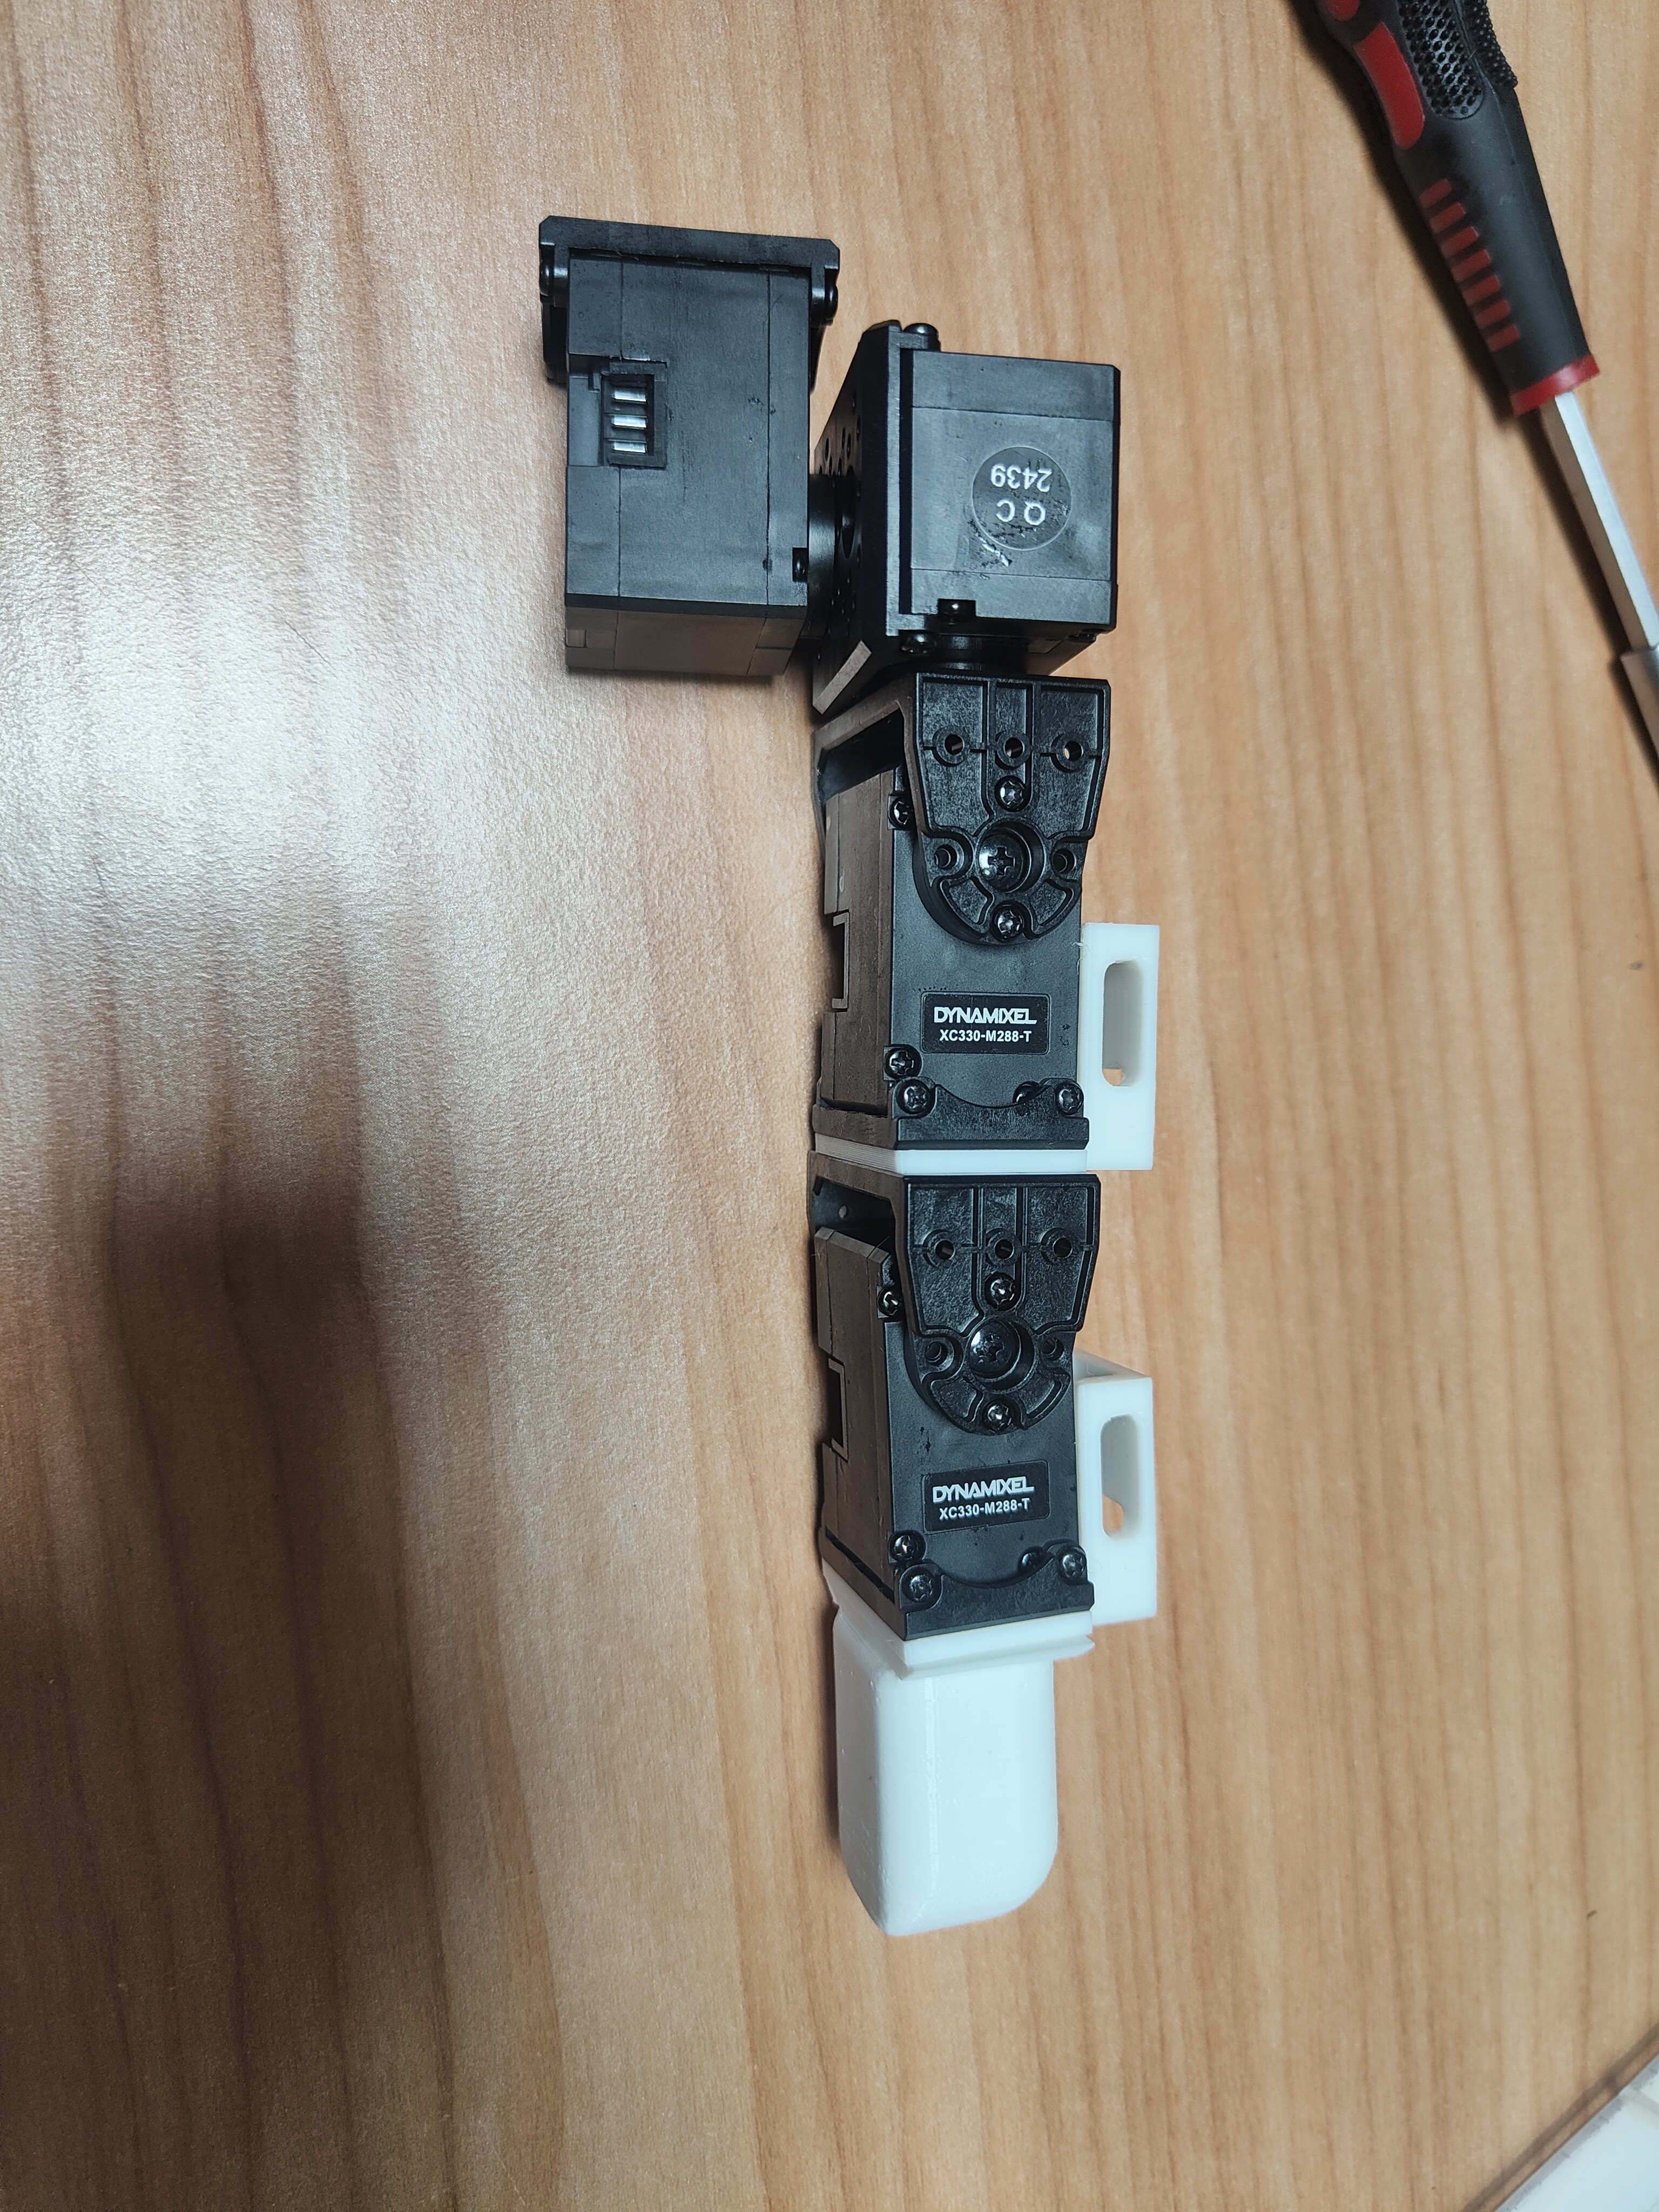
\includegraphics[height=6cm]{figs/chapter4/polegar.jpg}
        \caption{Polegar construído de acordo com a Documentação da Leap Hand}
        \label{fig:polegar}
    \end{minipage}
    \hfill
    \begin{minipage}[b]{0.45\textwidth}
        \centering
        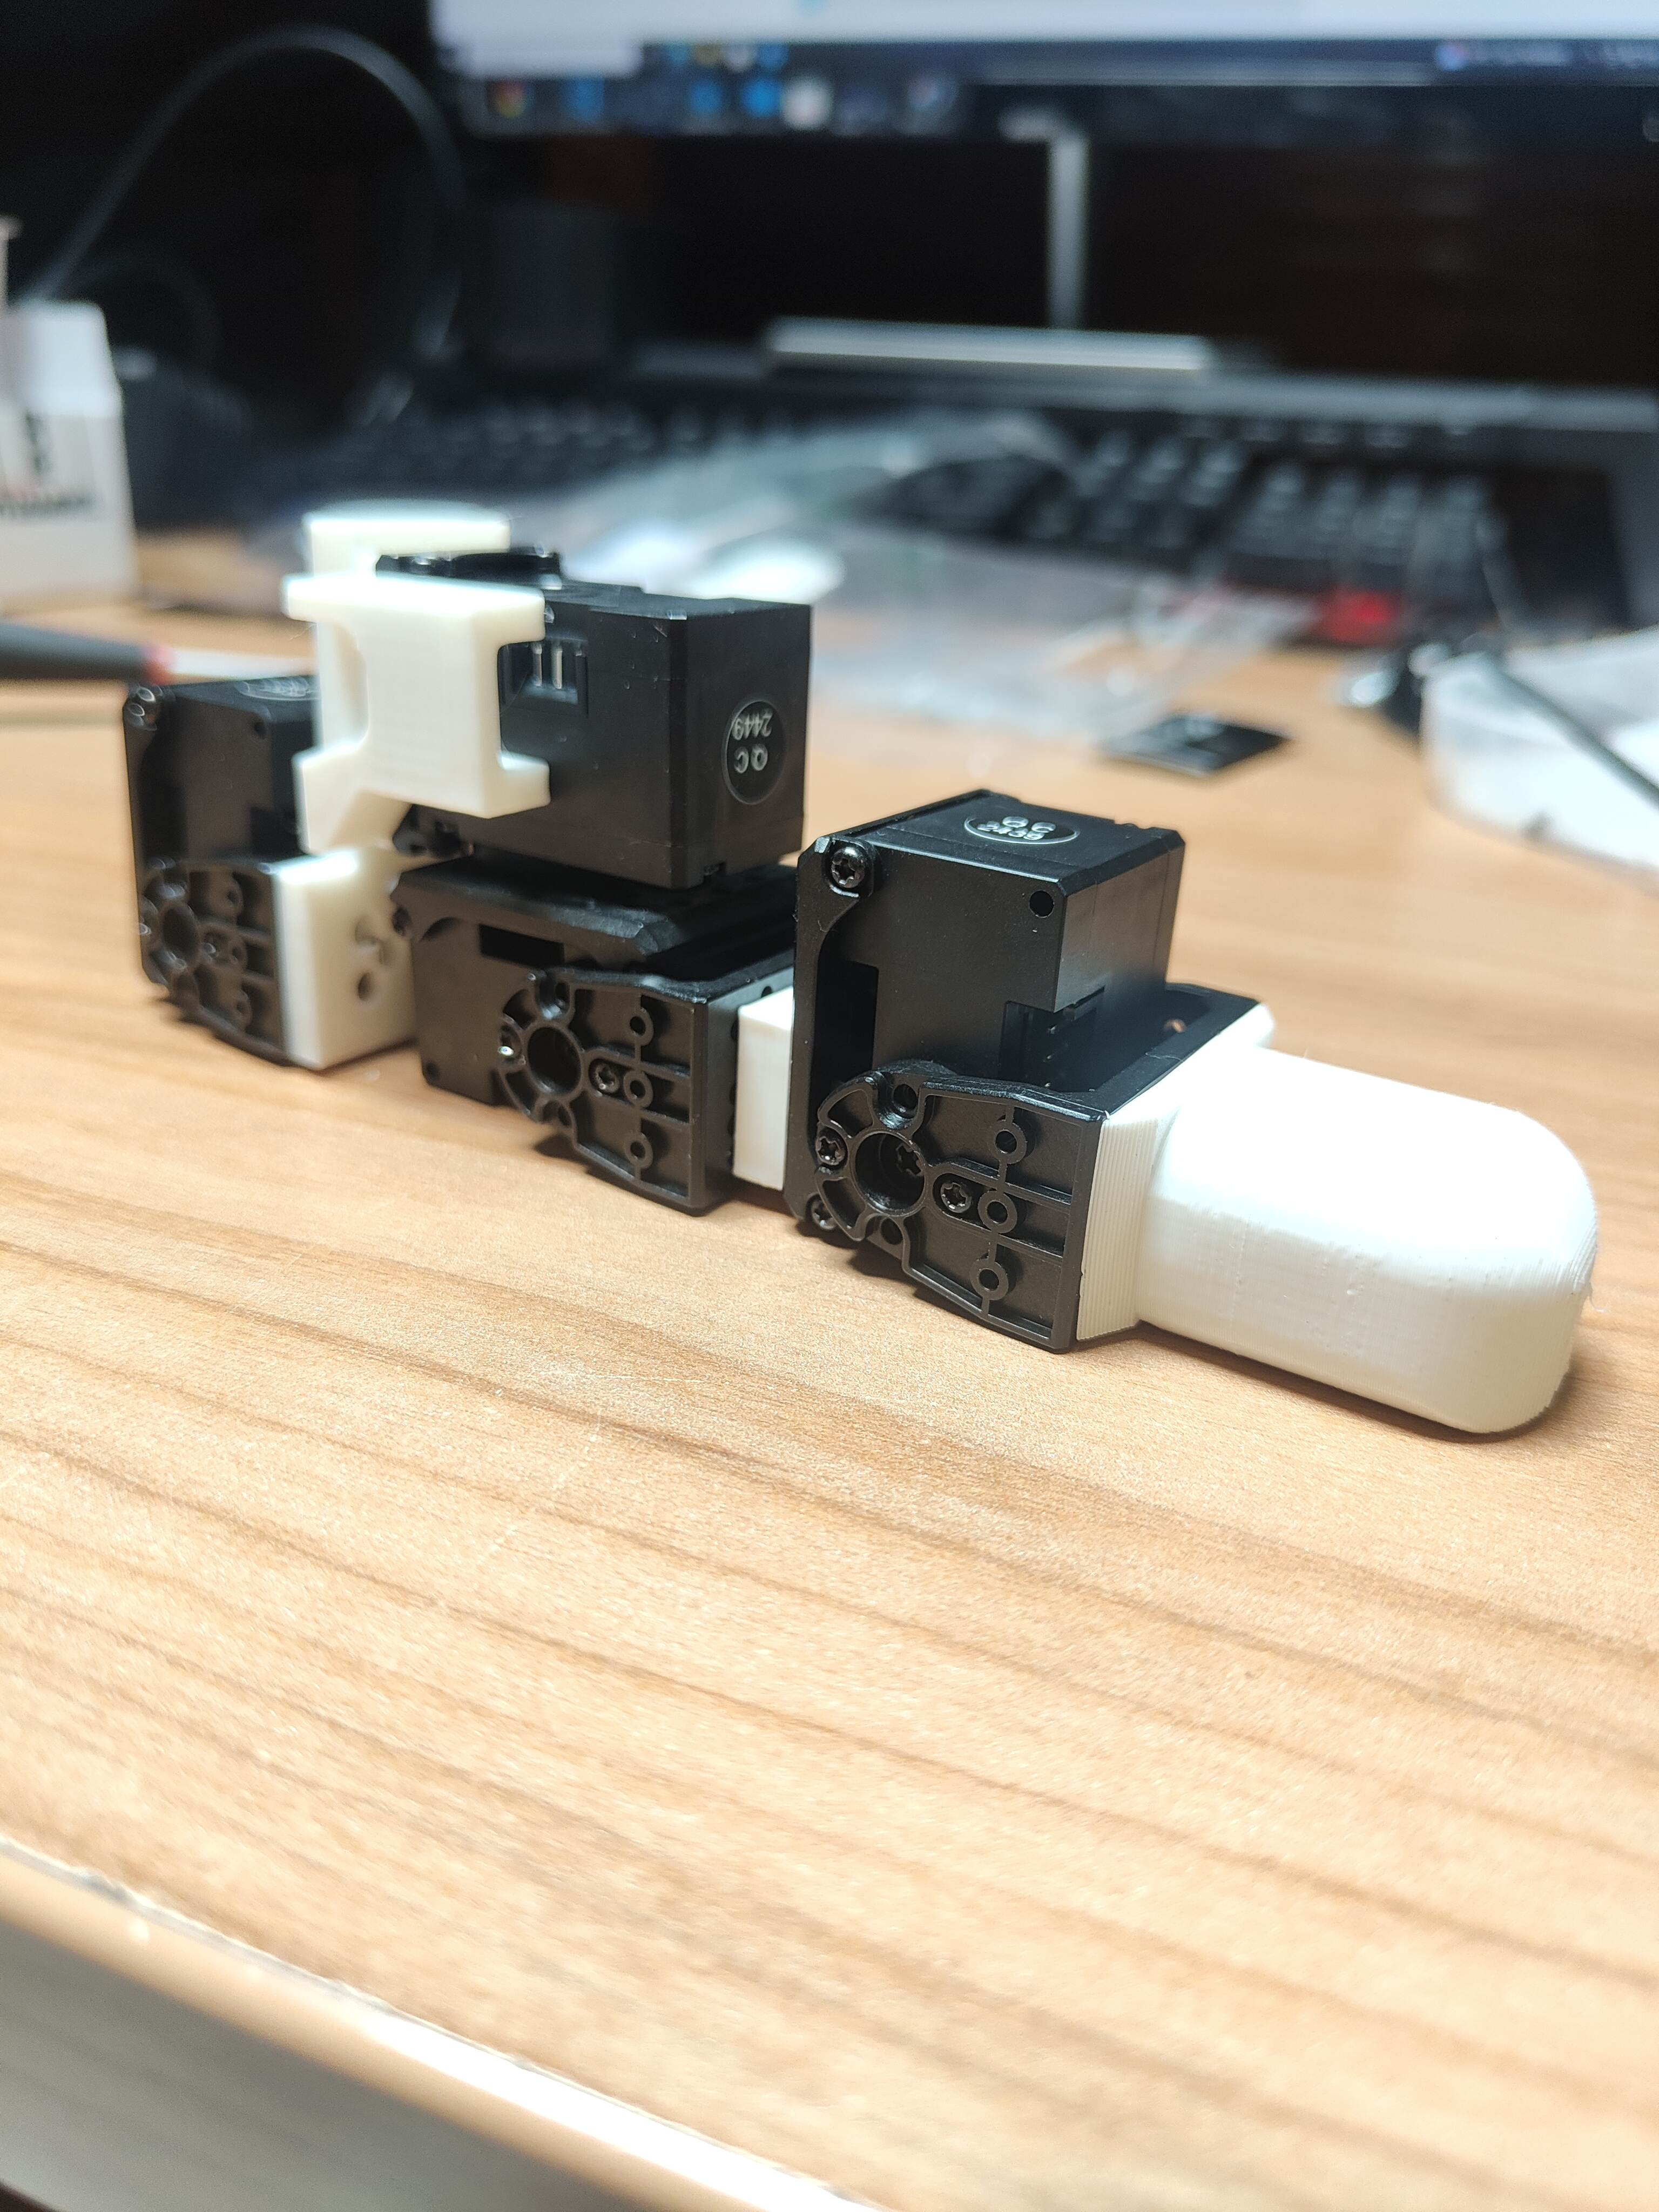
\includegraphics[height=6cm]{figs/chapter4/dedo.jpg}
        \caption{Dedo construído de acordo com a documentação da Leap Hand correspondente à estrutura do dedo indicador, médio e anelar}
        \label{fig:dedo}
    \end{minipage}
\end{figure}

No final do processo, obteve-se a mão totalmente montada, de acordo com a estrutura proposta na LEAP Hand, conforme ilustrado na Figura~\ref{fig:mao_montada}.

\begin{figure}[H]
    \centering
    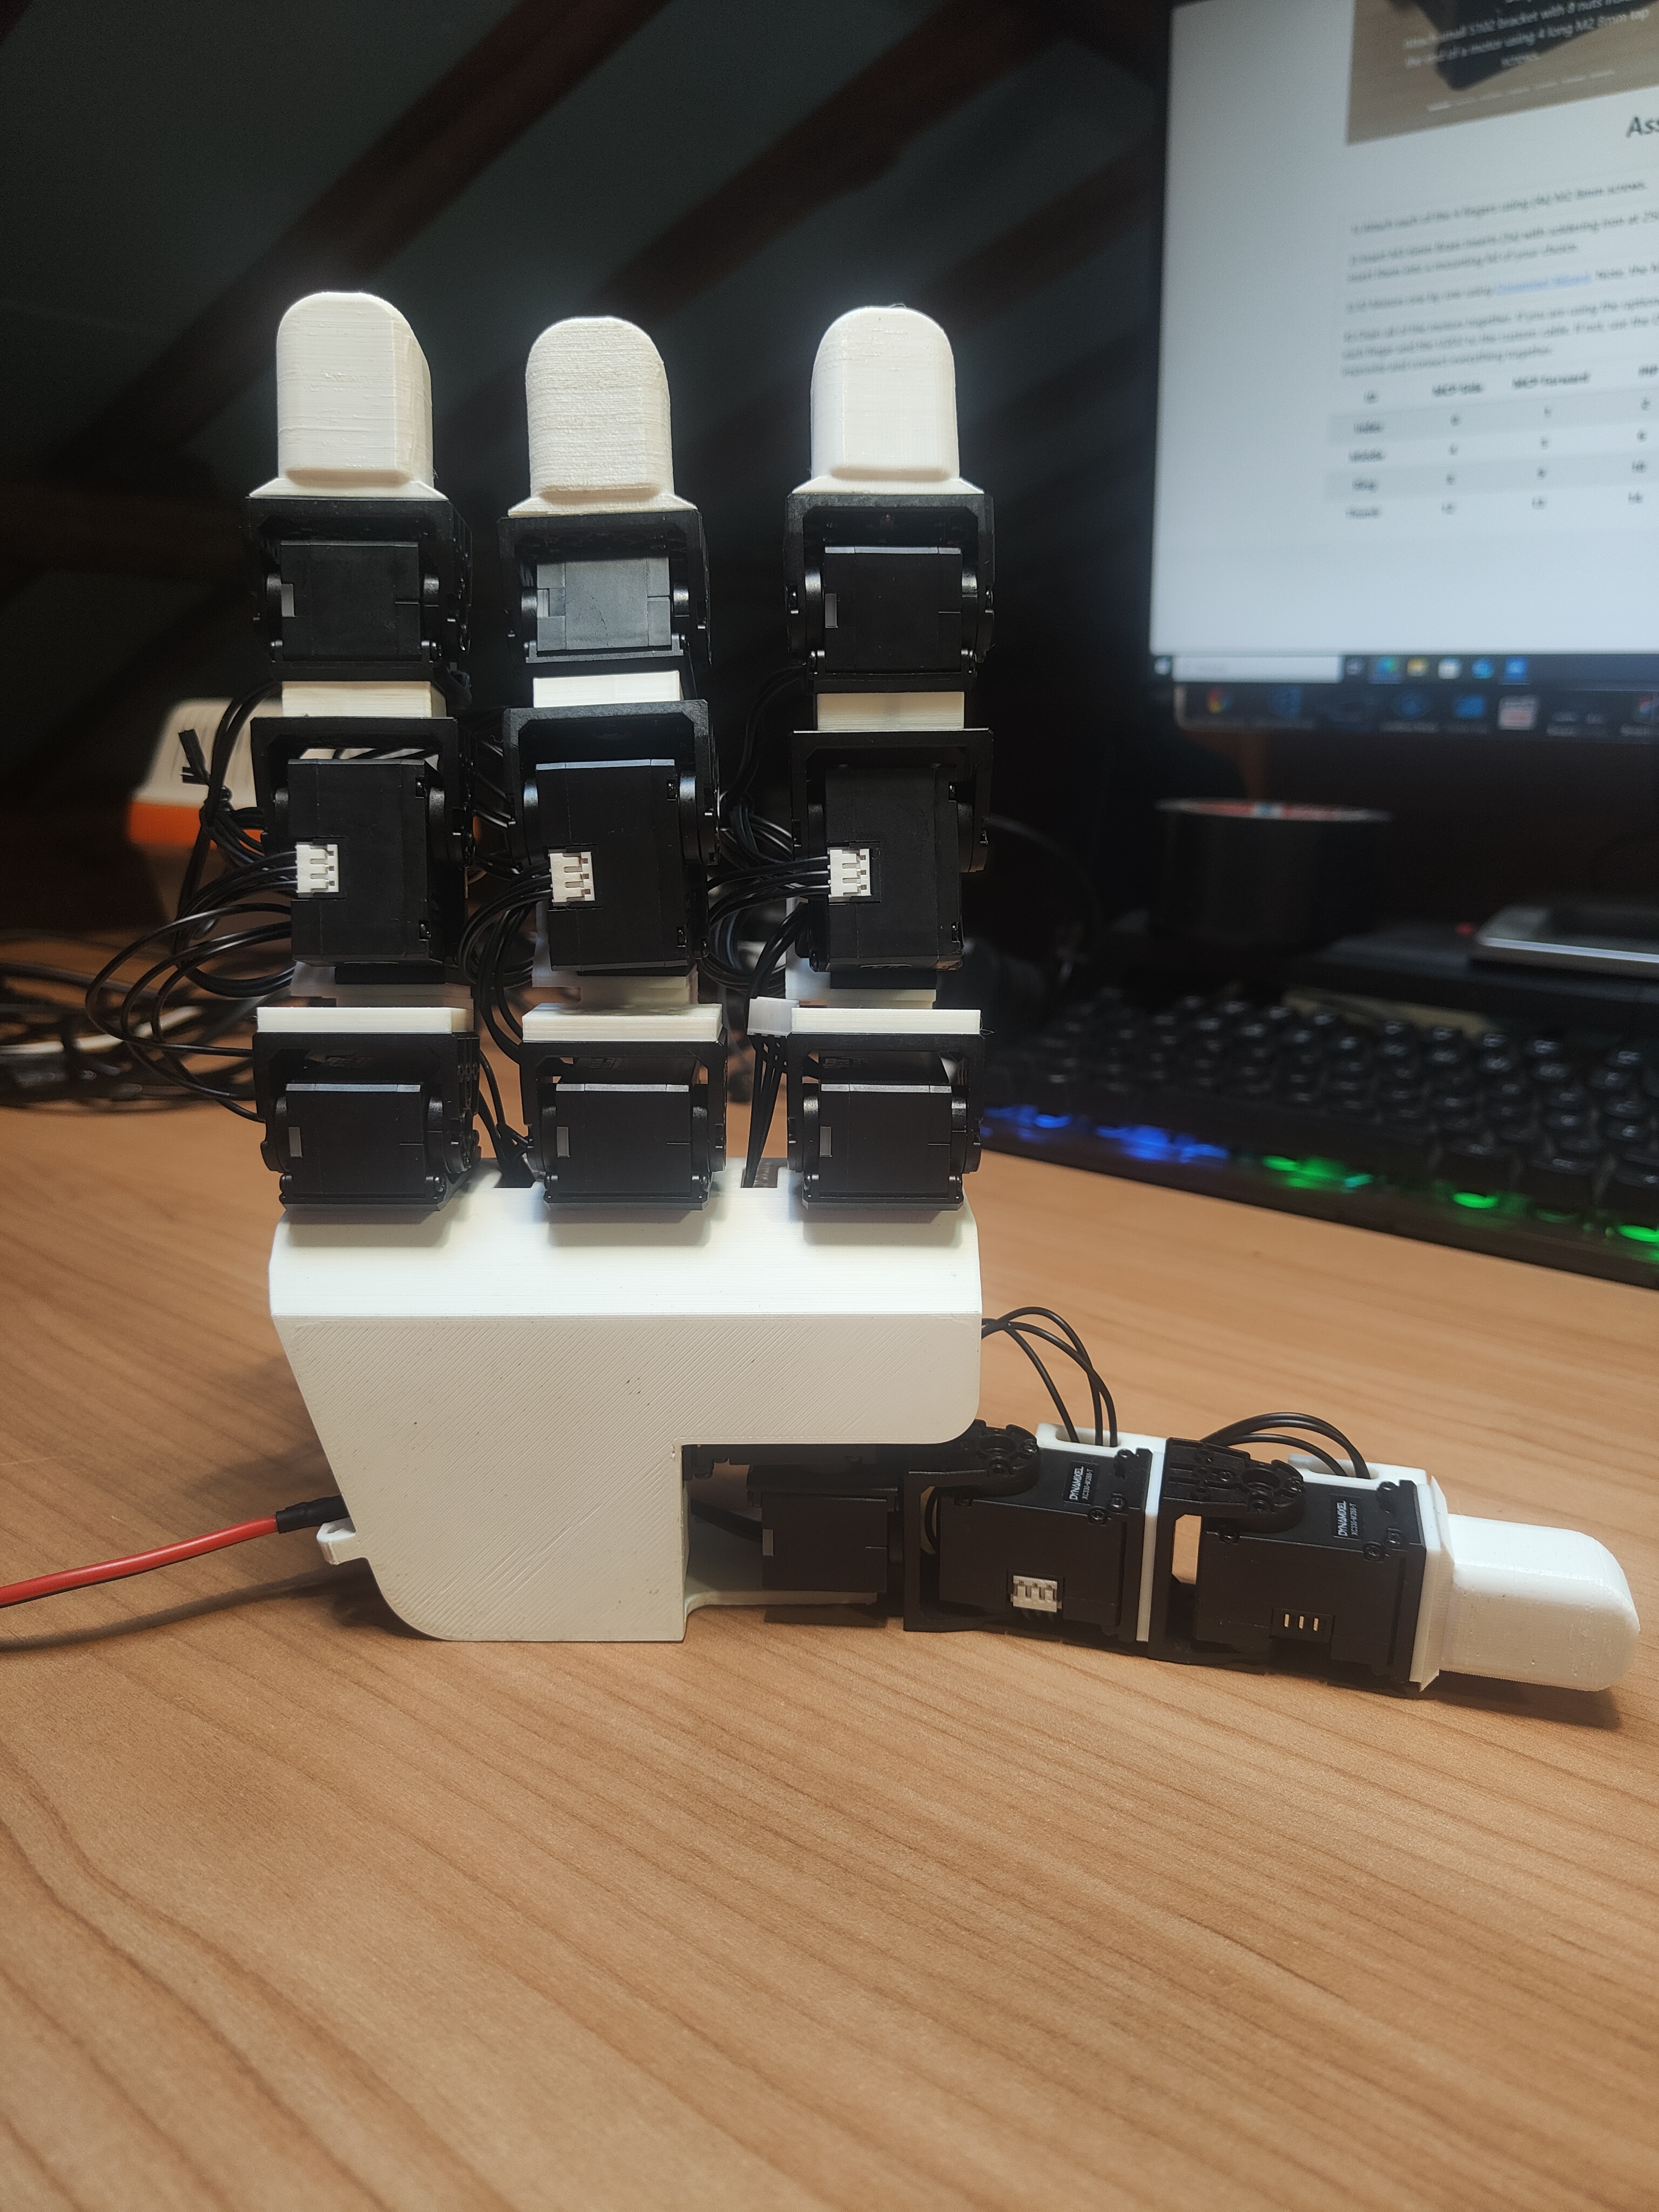
\includegraphics[height=8cm]{figs/chapter4/leap.jpg}
    \caption{Mão robótica completamente montada, seguindo a estrutura proposta na documentação da LEAP Hand.}
    \label{fig:mao_montada}
    
\end{figure}

Para complementar a descrição deste processo, no Apêndice~\ref{appendix:montagem_polegar} e ~\ref{appendix:montagem_dedo} e  são apresentadas imagens sequenciais representativas da construção de cada dedo, bem como hiperligações~\ref{appendix:videos} para vídeos que documentam o procedimento completo de montagem, constituindo assim um apoio visual adicional à documentação escrita.



Embora a montagem inicial tenha seguido rigorosamente as orientações da documentação da LEAP Hand, durante o desenvolvimento do projeto surgiram necessidades específicas que motivaram adaptações à estrutura original. Estas modificações serão detalhadas nas secções seguintes deste capítulo.



\subsection{Configuração dos Motores}

Antes de iniciar o desenvolvimento do código responsável pelo controlo dos movimentos da mão robótica, foi necessário proceder à configuração inicial dos motores Dynamixel. Esta fase incluiu a atribuição de identificadores únicos (IDs) a cada motor, uma vez que todos os motores, por defeito, vêm configurados com o mesmo ID. Para isso, recorreu-se à ferramenta gráfica Dynamixel Wizard 2.0, que permite, de forma intuitiva, alterar os parâmetros fundamentais de cada atuador.

Nesta configuração inicial, os IDs atribuídos seguiram a mesma lógica utilizada na documentação da LEAP Hand, garantindo assim compatibilidade com a estrutura de referência proposta pelos autores.

\subsubsection{Modos de Operação do Motores Dynamixel}

Após a atribuição dos IDs a cada motor, foi necessário configurar o modo de operação correspondente. Os motores Dynamixel XC330-M288-T suportam diversos modos de funcionamento, permitindo adaptá-los a diferentes tipos de movimentos e estratégias de controlo.

Na presente subsecção, são descritos os principais modos de operação disponibilizados por estes atuadores, destacando as suas características e o comportamento em situações com ou sem contacto com obstáculos.


\begin{enumerate}
    \item \textbf{Position Control Mode} \\
    Este modo permite definir uma posição angular específica que o motor deve atingir, dentro dos limites físicos configurados. Caso surja um obstáculo durante o movimento, o motor continuará a aplicar torque máximo na tentativa de alcançar a posição desejada, o que pode levar ao sobreaquecimento dos motores.


    \item \textbf{Extended Position Control Mode} \\
    Uma extensão do modo anterior, permite rotações superiores a 360°, tornando-se útil para aplicações que requerem movimento contínuo em rotação. No entanto, não é relevante no contexto deste projeto, dado que as juntas dos dedos não realizam rotações completas.


    \item \textbf{Velocity Control Mode} \\  
    Este modo permite definir uma velocidade angular constante, sem especificar uma posição final. O motor acelera até atingir a velocidade pretendida e mantém-se em rotação. Na presença de um obstáculo, o motor continua a tentar girar, aplicando o torque máximo, o que pode resultar em sobreaquecimento.


    \item \textbf{PWM Control Mode} \\
    Permite controlar diretamente a potência fornecida ao motor através de modulação por largura de pulso (PWM). Este modo oferece um controlo mais direto e flexível, mas não garante precisão de movimento, nem proteção contra obstáculos, podendo causar sobreaquecimento em situações de bloqueio mecânico.


    \item \textbf{Current Control Mode} \\
    Neste modo, controla-se diretamente o torque aplicado ao definir a corrente desejada. Se não houver resistência, o motor continua a girar. Na presença de um obstáculo, o motor não tenta forçar o movimento, e mantém um torque constante correspondente ao valor de corrente definido, oferecendo uma resposta segura e previsível.


    \item \textbf{Current-Based Position Control Mode} \\   
    Combina as vantagens do controlo de posição com limitação de corrente. O motor tenta alcançar uma determinada posição, mas limita o torque máximo aplicado, de acordo com o valor de corrente permitido. Se o obstáculo exigir mais torque do que o configurado, o motor interrompe o movimento, mantendo a força aplicada constante.

\end{enumerate}

A Tabela~\ref{tab:modos_operacao} resume os diferentes modos de operação, destacando os parâmetros controlados, as aplicações ideais e o comportamento em situações de contacto com obstáculos:

\begin{table}[H]
\centering
\begin{tabular}{l l p{6cm}}
\toprule
\textbf{Modo} & \textbf{Controla}  & \textbf{Reação a Obstáculos} \\
\midrule
Position Control & Posição & Aplica torque máximo até atingir posição \\
Extended Position & Posição ($>$360º) & Idêntico ao Position Control \\
Velocity Control & Velocidade  & Aplica torque máximo para manter velocidade \\
Current Control & Corrente (torque) & Mantém torque constante, sem tentar forçar \\
Current-Based Position & Posição + Corrente & Tenta atingir posição, mas respeita limite de torque \\
PWM Control & Potência (PWM) & Não protege contra sobrecarga ou obstáculos \\
\bottomrule
\end{tabular}
\caption{Resumo dos modos de operação dos motores Dynamixel}
\label{tab:modos_operacao}
\end{table}

A escolha do modo de operação adequado é essencial para garantir o desempenho desejado e a segurança do sistema. No contexto deste projeto, onde o contacto com objetos e a necessidade de limitar a força aplicada pelos dedos são aspetos fundamentais, foi escolhido o \textit{Current-Based Position Control Mode}, uma vez que este modo permite controlar a posição de cada articulação, ao mesmo tempo que impõe um limite ao torque aplicado, o que evita danos em situações de bloqueio ou contacto inesperado.


\subsection{Programação e Controlo}

A implementação do controlo dos motores Dynamixel exige, numa fase inicial, a correta definição dos parâmetros de comunicação, de forma a garantir a fiabilidade da ligação entre o sistema computacional e os atuadores.

Entre os elementos essenciais a configurar, destaca-se a especificação da porta serial utilizada, tipicamente \texttt{/dev/ttyUSB0} em sistemas operativos baseados em Linux, a taxa de transmissão de dados (\textit{baud rate}), o protocolo de comunicação (sendo utilizada a versão 2.0), a série dos motores (neste caso, a série X, correspondente aos modelos Dynamixel XC330-M288-T) e o identificador único (\textit{ID}) atribuído previamente a cada motor.

A correta parametrização destes elementos é fundamental para que seja possível estabelecer comunicação com os motores, enviar comandos de controlo e ler os parâmetros relevantes de operação. Nos pontos seguintes, descreve-se de forma progressiva a programação de um motor individual, o controlo coordenado de um dedo completo e, por fim, a implementação da lógica de controlo da mão robótica na sua totalidade.



\subsubsection{Programação de um motor individual}


A programação de um motor individual constitui o primeiro passo no desenvolvimento da lógica de controlo da mão robótica.
O processo tem início com a importação da biblioteca e a configuração da interface de comunicação serial. Tal configuração é efetuada através da criação dos objetos \texttt{portHandler} e \texttt{packetHandler}, com as instruções \texttt{portHandler = PortHandler(DEVICENAME)} e \texttt{packetHandler = PacketHandler(PROTOCOL\_VERSION)}. O primeiro estabelece a ligação física à porta serial especificada (por exemplo, \texttt{/dev/ttyUSB0}), enquanto o segundo gere a codificação e descodificação dos pacotes de dados, de acordo com o protocolo de comunicação adotado (neste projeto, a versão 2.0).


Após a abertura da porta e a verificação do sucesso da ligação, é necessário ativar o torque do motor para que este possa responder aos comandos enviados. A partir deste momento, torna-se possível controlar diversos parâmetros do motor, como a posição, a velocidade e a corrente máxima, dependendo do modo de operação previamente selecionado.

A leitura e escrita desses parâmetros nos registos internos do motor são realizadas através das funções disponibilizadas pelo SDK. A leitura pode abranger dados como a posição atual, velocidade de rotação, corrente consumida ou valor de PWM. A escolha da função adequada depende da dimensão dos dados a transferir, sendo comum o uso de \texttt{read2ByteTxRx()} e \texttt{read4ByteTxRx()} para valores de 2 e 4 bytes, respetivamente.

É importante salientar que os motores Dynamixel não fornecem diretamente a posição angular em graus ou radianos. Em vez disso, utilizam um sistema interno de representação baseado em \textit{ticks}, no qual a posição é expressa por um valor inteiro. No caso do modelo \texttt{XC330-M288-T}, a resolução do encoder é de 12 bits, o que resulta em $2^{12} = 4096$ valores distintos ao longo de uma rotação completa de $360^\circ$. Deste modo, cada unidade (\textit{tick}) corresponde a um incremento angular de aproximadamente $0{,}088^\circ$.

A conversão do valor lido, em \textit{ticks}, para a correspondente posição angular em graus é efetuada através da equação~\eqref{eq:conversao_graus}:

\begin{equation}
\theta = \frac{360 \times \text{ticks}}{4096}
\label{eq:conversao_graus}
\end{equation}

onde $\theta$ representa a posição angular em graus, e \texttt{ticks} é o valor devolvido diretamente pelo motor.

De forma análoga, a velocidade de rotação também é representada em \textit{ticks}. Neste caso, a relação com as unidades físicas é definida por um fator de conversão fornecido pelo fabricante. Para o motor em questão, cada unidade corresponde a aproximadamente 0{,}229 rotações por minuto (RPM). Assim, a velocidade real pode ser obtida através da equação~\eqref{eq:conversao_rpm}:

\begin{equation}
\text{Velocidade (RPM)} = \text{ticks} \times 0.229
\label{eq:conversao_rpm}
\end{equation}

Adicionalmente, o sinal do valor atribuído à velocidade determina o sentido de rotação: valores positivos indicam rotação no sentido horário, enquanto valores negativos correspondem a uma rotação no sentido anti-horário.

No que diz respeito à corrente elétrica consumida pelo motor, esta é diretamente disponibilizada pelo SDK em miliamperes (mA), não sendo necessária qualquer conversão adicional. Este parâmetro está diretamente relacionado com o torque aplicado pelo motor, sendo, por isso, relevante para o diagnóstico do esforço mecânico exigido durante o funcionamento.


\subsubsection{Programação e Controlo de um dedo}

Após a compreensão do funcionamento individual dos motores Dynamixel e da configuração dos seus parâmetros, procedeu-se ao desenvolvimento do controlo coordenado de um dedo completo da mão robótica. Cada dedo integra quatro motores, tornando necessário garantir a leitura sincronizada dos seus estados e o envio simultâneo de comandos de controlo, de forma eficiente e escalável.

Para tal, recorreu-se às funcionalidades de comunicação em bloco disponibilizadas pelo Dynamixel SDK, nomeadamente as operações \texttt{sync\_read}, \texttt{sync\_write}, \texttt{bulk\_read} e \texttt{bulk\_write}. No que respeita à leitura dos parâmetros dos motores — posição, velocidade e corrente — a função \texttt{sync\_read} foi a selecionada, por permitir aceder a um mesmo conjunto de registos em múltiplos motores de forma síncrona. Esta abordagem revelou-se eficiente tanto em termos de desempenho como de utilização de memória, além de respeitar as limitações de tamanho de mensagem impostas pelo protocolo de comunicação, evitando os riscos associados à utilização do \texttt{bulk\_read}.

Relativamente à escrita de comandos, optou-se pela função \texttt{bulk\_write}, que permite enviar dados distintos para registos diferentes de múltiplos motores numa única operação. Apesar de o registo alvo ser frequentemente o mesmo (como a posição ou o limite de corrente), esta escolha confere maior versatilidade ao sistema, permitindo a sua adaptação a cenários futuros em que diferentes parâmetros possam ser configurados seletivamente em cada motor.

Assim, a combinação de \texttt{sync\_read} para a leitura periódica do estado dos motores e \texttt{bulk\_write} para o envio de comandos de controlo assegura simultaneidade, escalabilidade e robustez no controlo coordenado de um dedo da mão robótica, servindo como base sólida para a extensão posterior ao controlo integrado de múltiplos dedos. Com esta abordagem, foi possível atingir uma taxa de leitura estável de aproximadamente 50Hz, garantindo uma monitorização suficientemente rápida para aplicações em tempo quase real.

Após implementar com sucesso o envio de comandos e a leitura simultânea dos parâmetros dos motores, procedeu-se à aplicação do modo de operação selecionado: o Current-Based Position Control Mode. A adaptação do código previamente desenvolvido foi direta, bastando configurar o registo correspondente ao modo de operação e definir um limite máximo de corrente na zona de inicialização do sistema. Esta configuração é realizada através da escrita nos endereços apropriados de cada motor Dynamixel.

Nos primeiros testes, foi definido um limite de corrente de 100mA. Embora este modo de operação não permita o controlo direto da velocidade, é possível estabelecer uma velocidade máxima por meio da configuração do parâmetro \texttt{Profile Velocity}. Assim, foram enviadas posições de destino previamente definidas para provocar o movimento de fecho e posterior abertura do dedo, com o objetivo de avaliar o comportamento dos motores em condições ideais. Os gráficos resultantes desta experiência encontram-se nas Figuras~\ref{fig:pos},~\ref{fig:vels} e ~\ref{fig:currs}.

\begin{figure}[H]
    \centering
    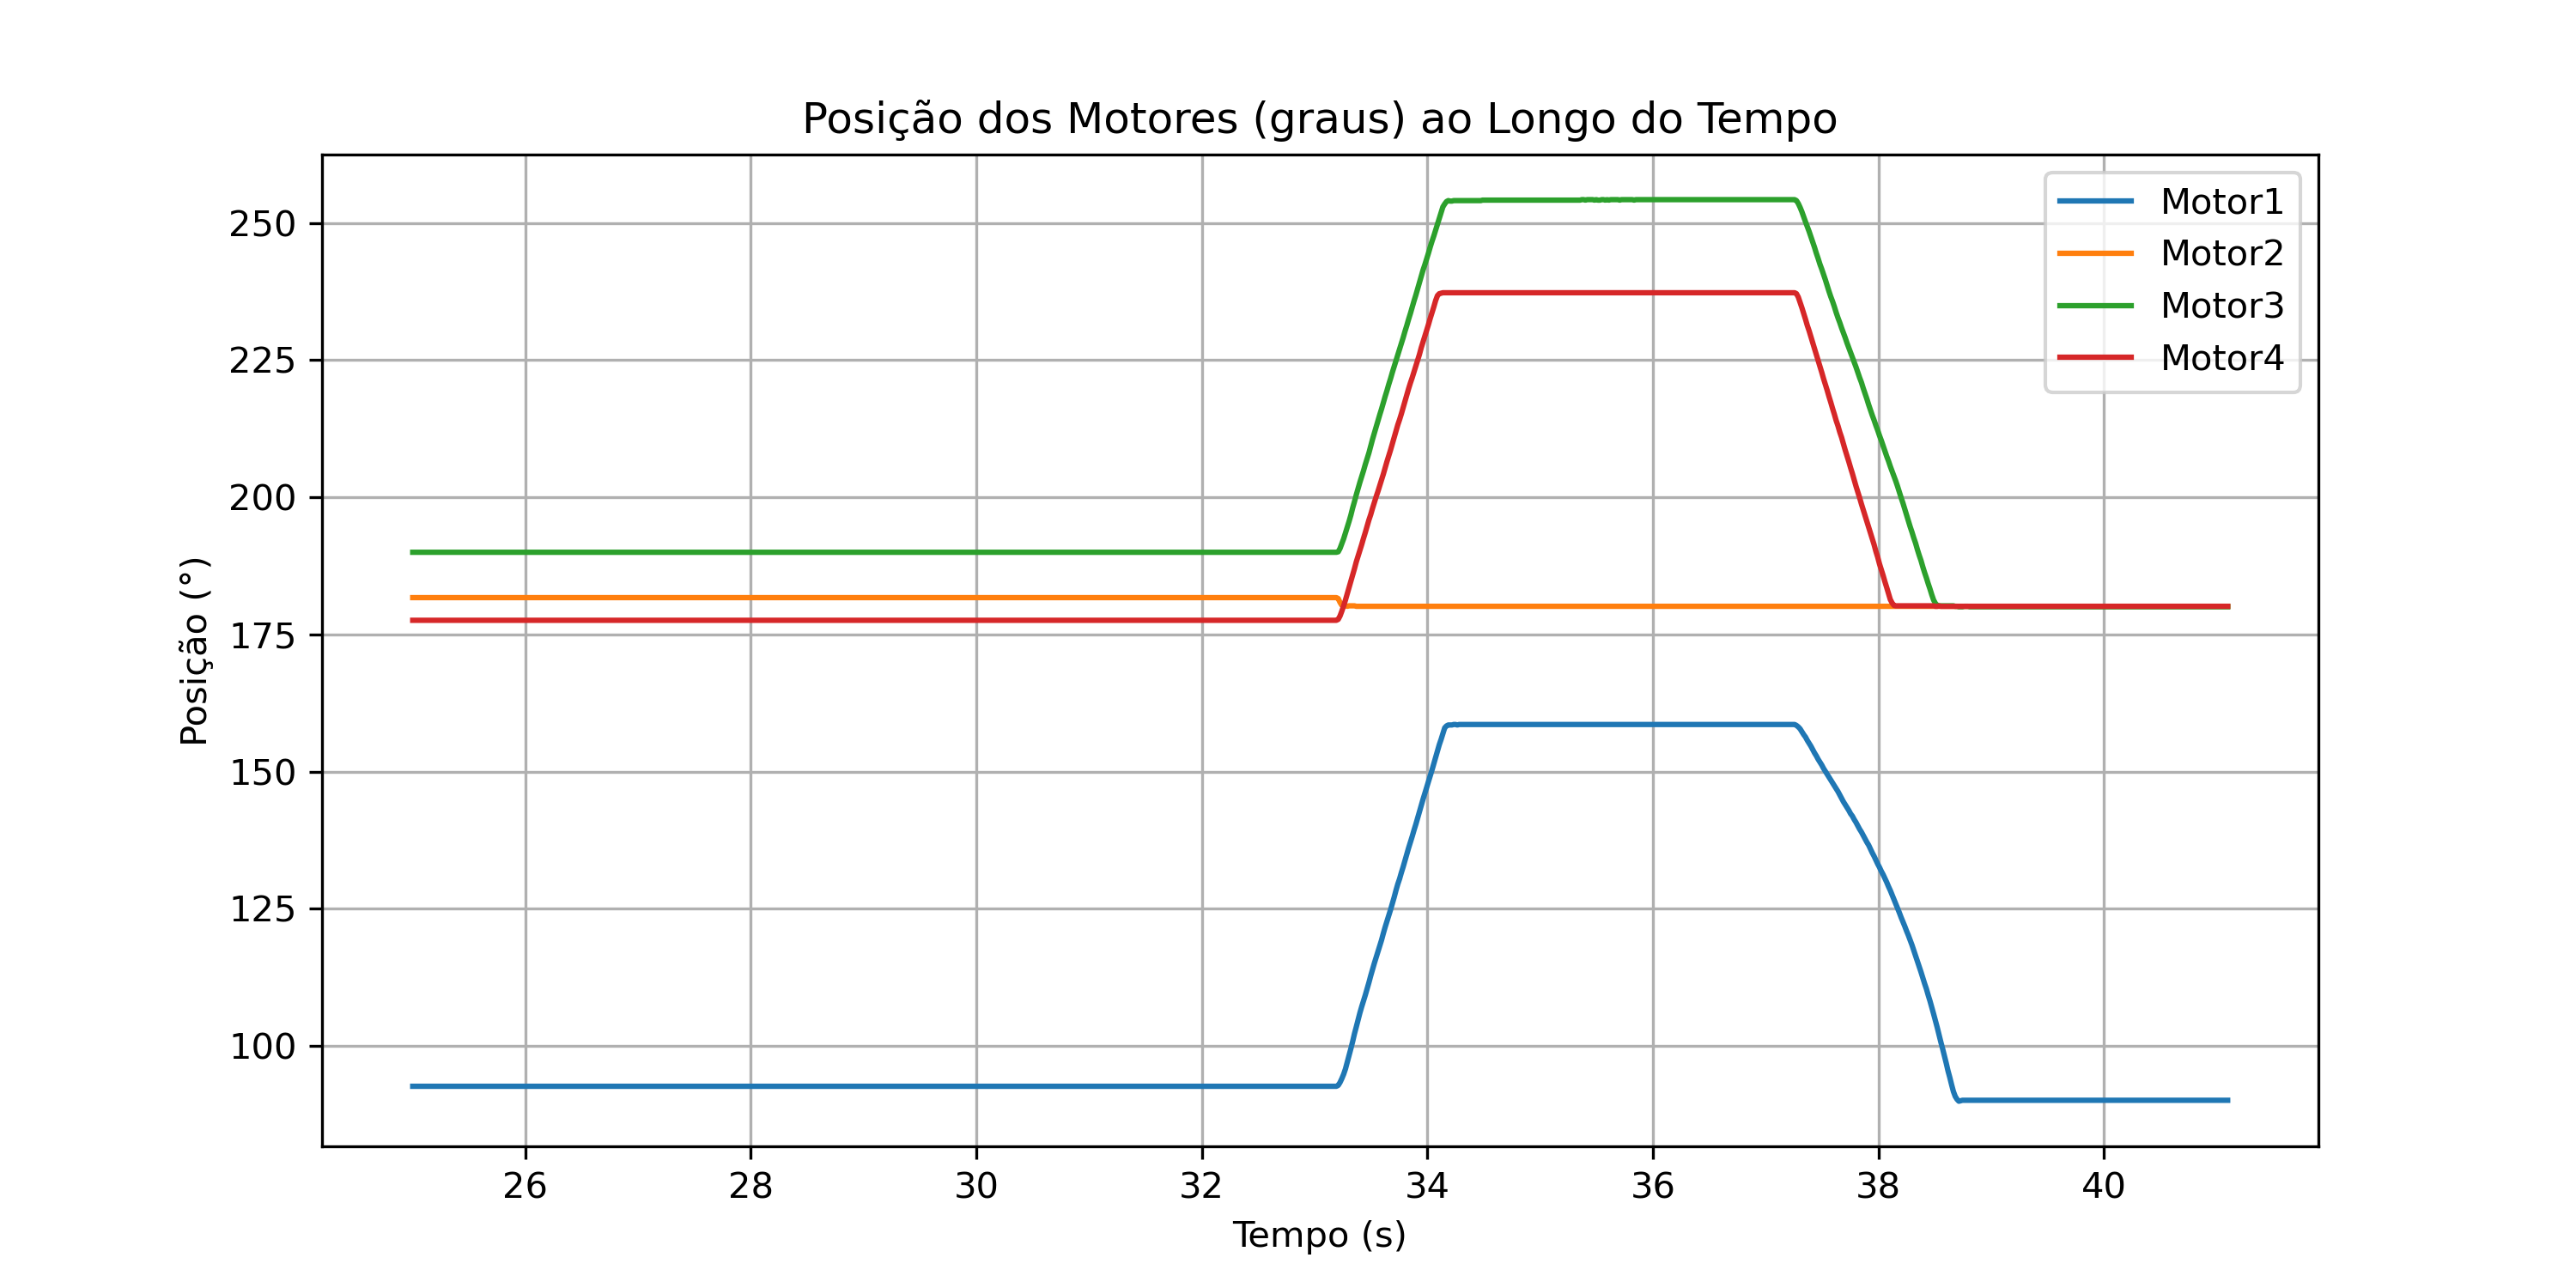
\includegraphics[height=6cm]{figs/chapter4/finger_positions.png}
    \caption{Posições dos motores ao longo do tempo durante o fecho e abertura do dedo sem nenhuma obstrução}
    \label{fig:pos}
    
\end{figure}
\begin{figure}[H]
    \centering
    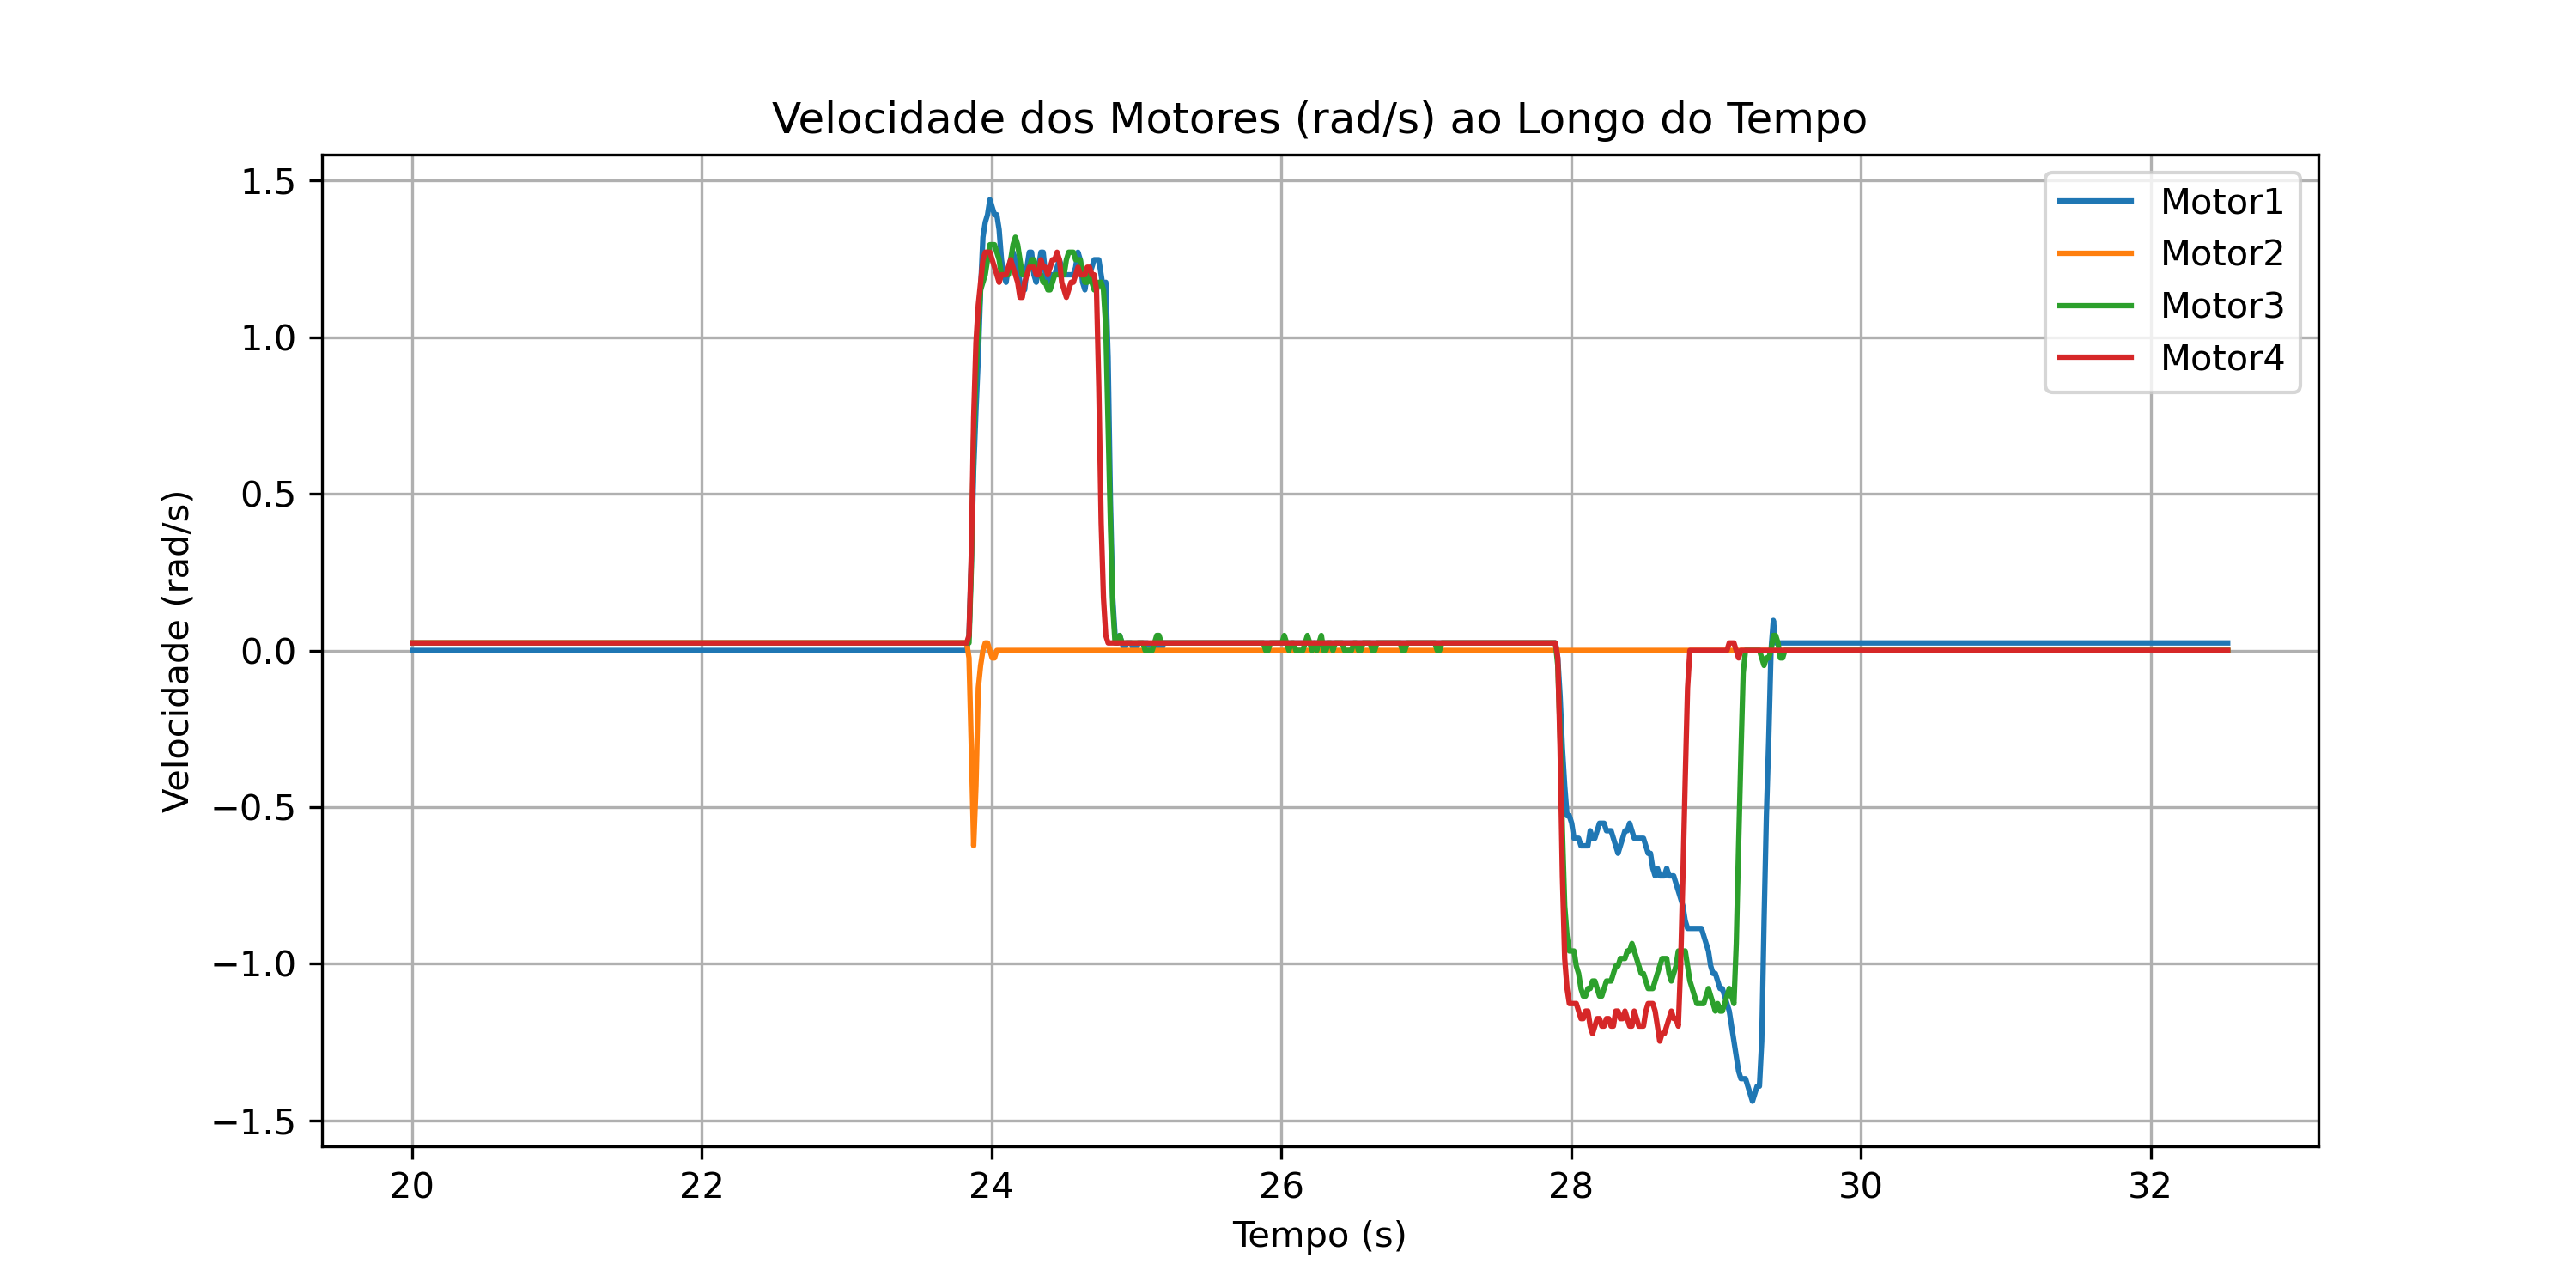
\includegraphics[height=6cm]{figs/chapter4/finger_velocities.png}
    \caption{Velocidades dos motores ao longo do tempo durante o fecho e abertura do dedo sem nenhuma obstrução}
    \label{fig:vels}
    
\end{figure}
\begin{figure}[H]
    \centering
    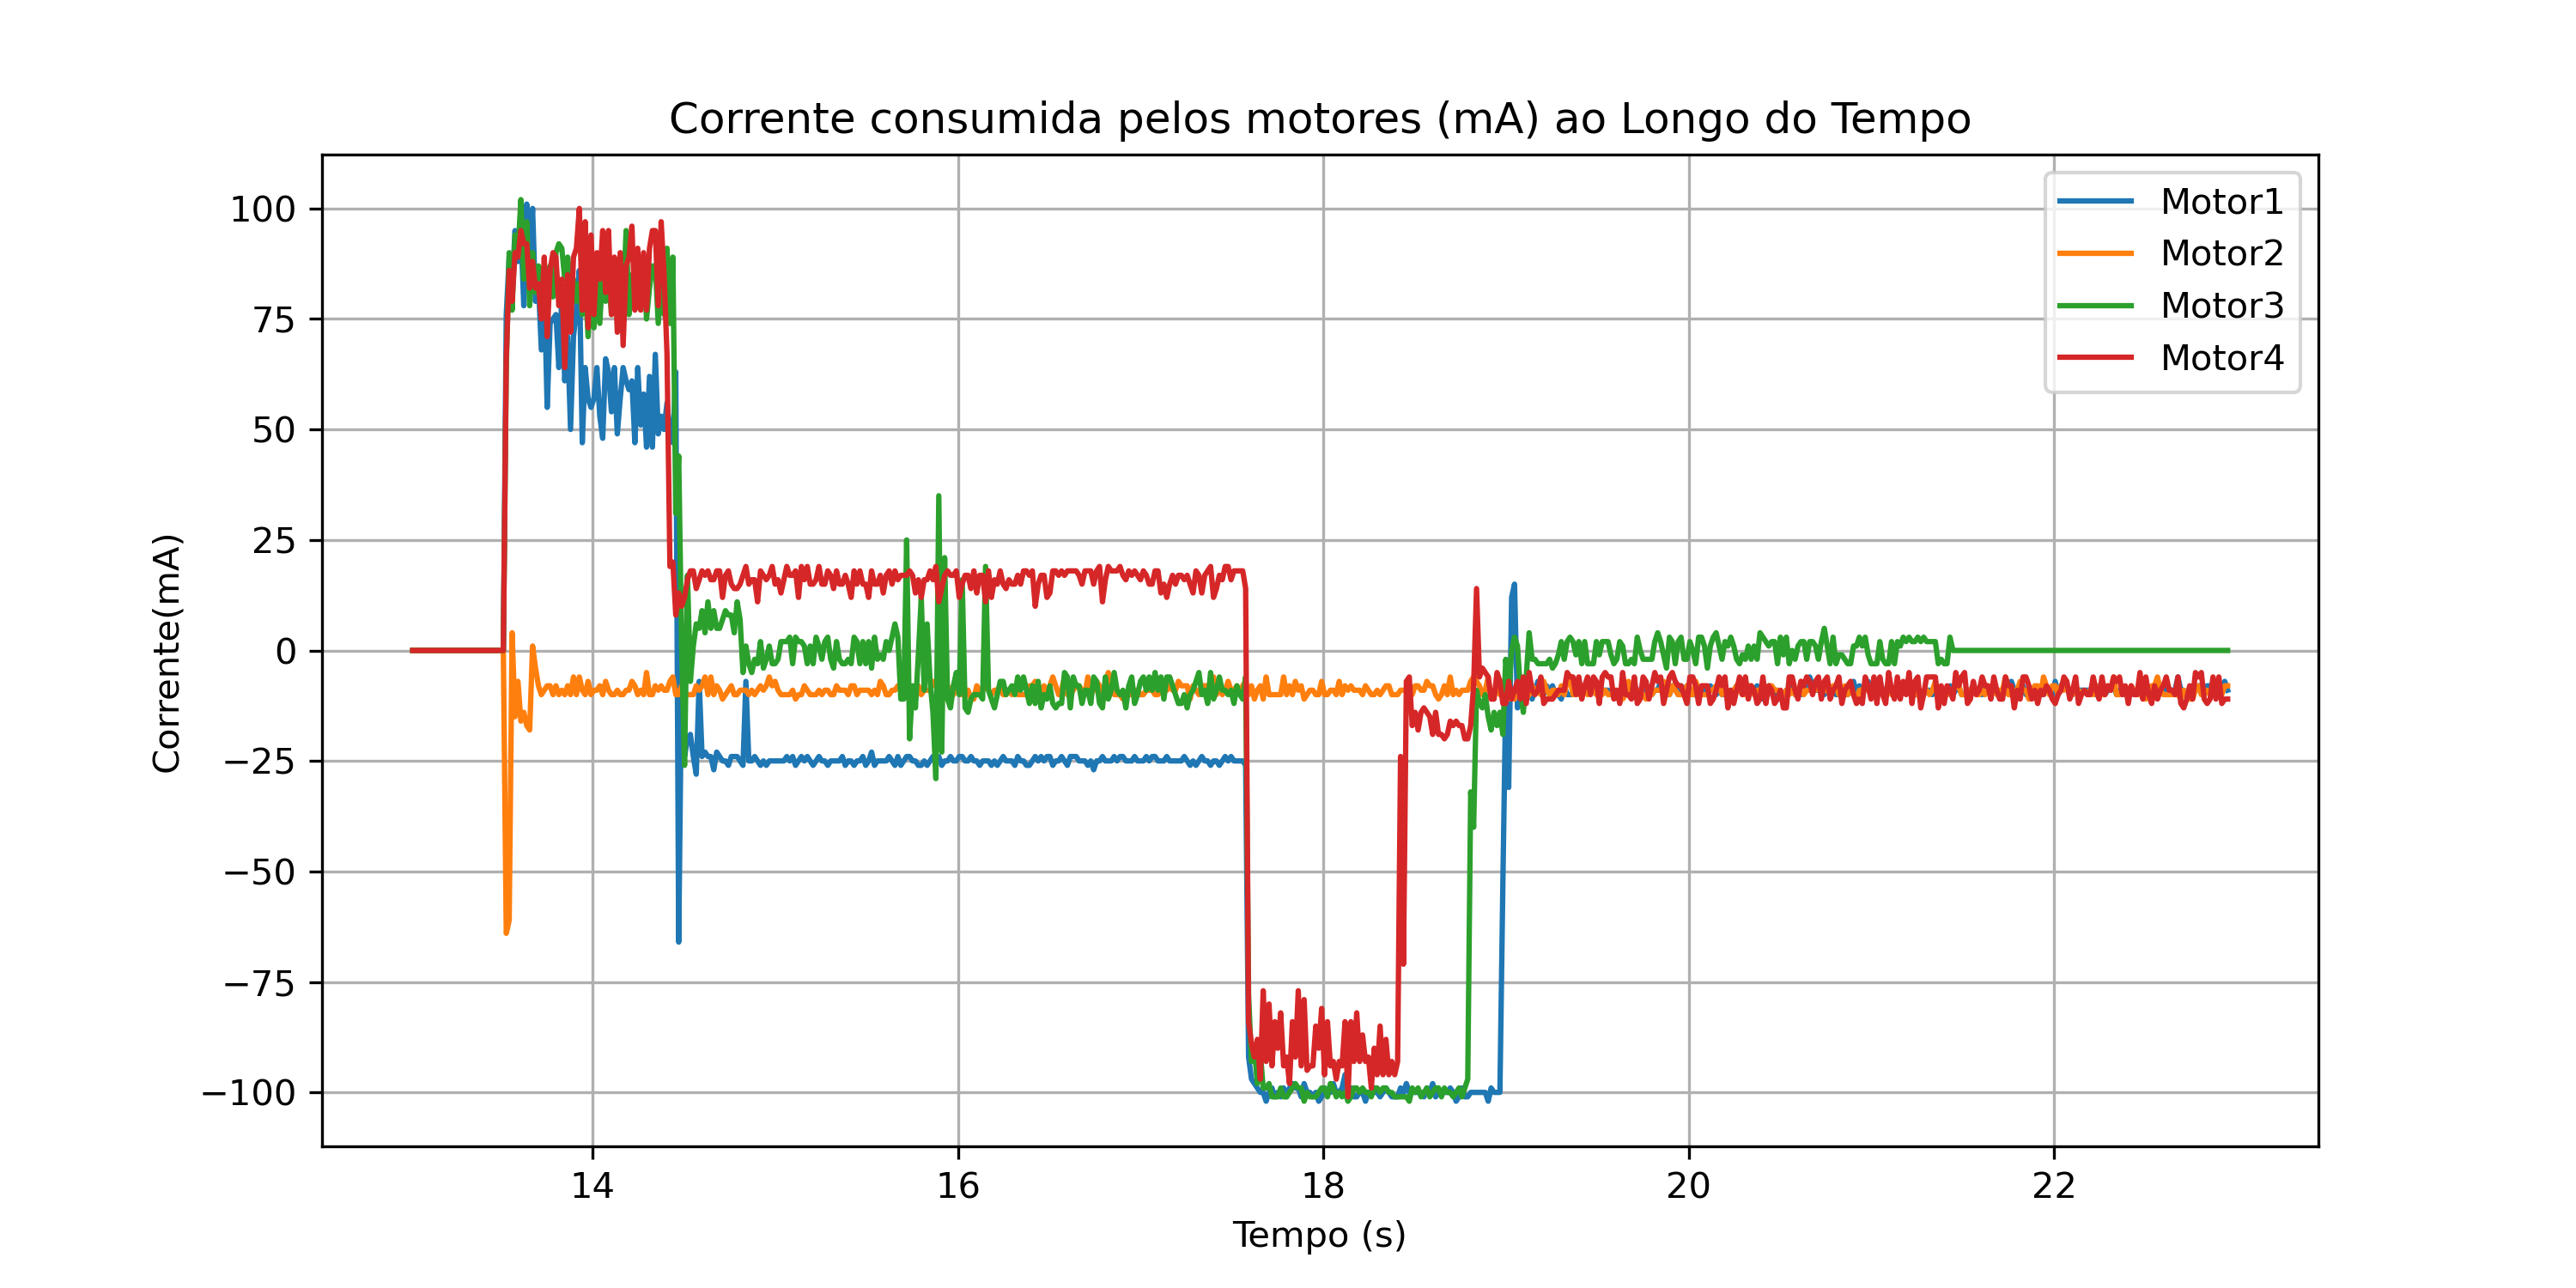
\includegraphics[height=6cm]{figs/chapter4/finger_currents.png}
    \caption{Correntes consumidas pelos motores ao longo do tempo durante o fecho e abertura do dedo sem nenhuma obstrução}
    \label{fig:currs}
    
\end{figure}

Como se pode observar, durante todo o movimento, os valores de corrente e velocidade mantiveram-se dentro dos limites especificados. A única exceção ocorreu no motor 1, onde se registou uma ligeira oscilação de velocidade, ultrapassando o valor definido em apenas 0.07 rad/s. Esta variação é considerada normal e esperada no funcionamento real dos motores, não comprometendo a estabilidade nem a segurança do sistema.

Na experiência seguinte, foram mantidas as mesmas posições de destino, mas introduziu-se um obstáculo físico que impedia a concretização do movimento pretendido. Tal como ilustrado nas Figuras~\ref{fig:pos1}, ~\ref{fig:vels1} e ~\ref{fig:currs1}, a análise dos dados revela diferenças claras entre os dois cenários. 

\begin{figure}[H]
    \centering
    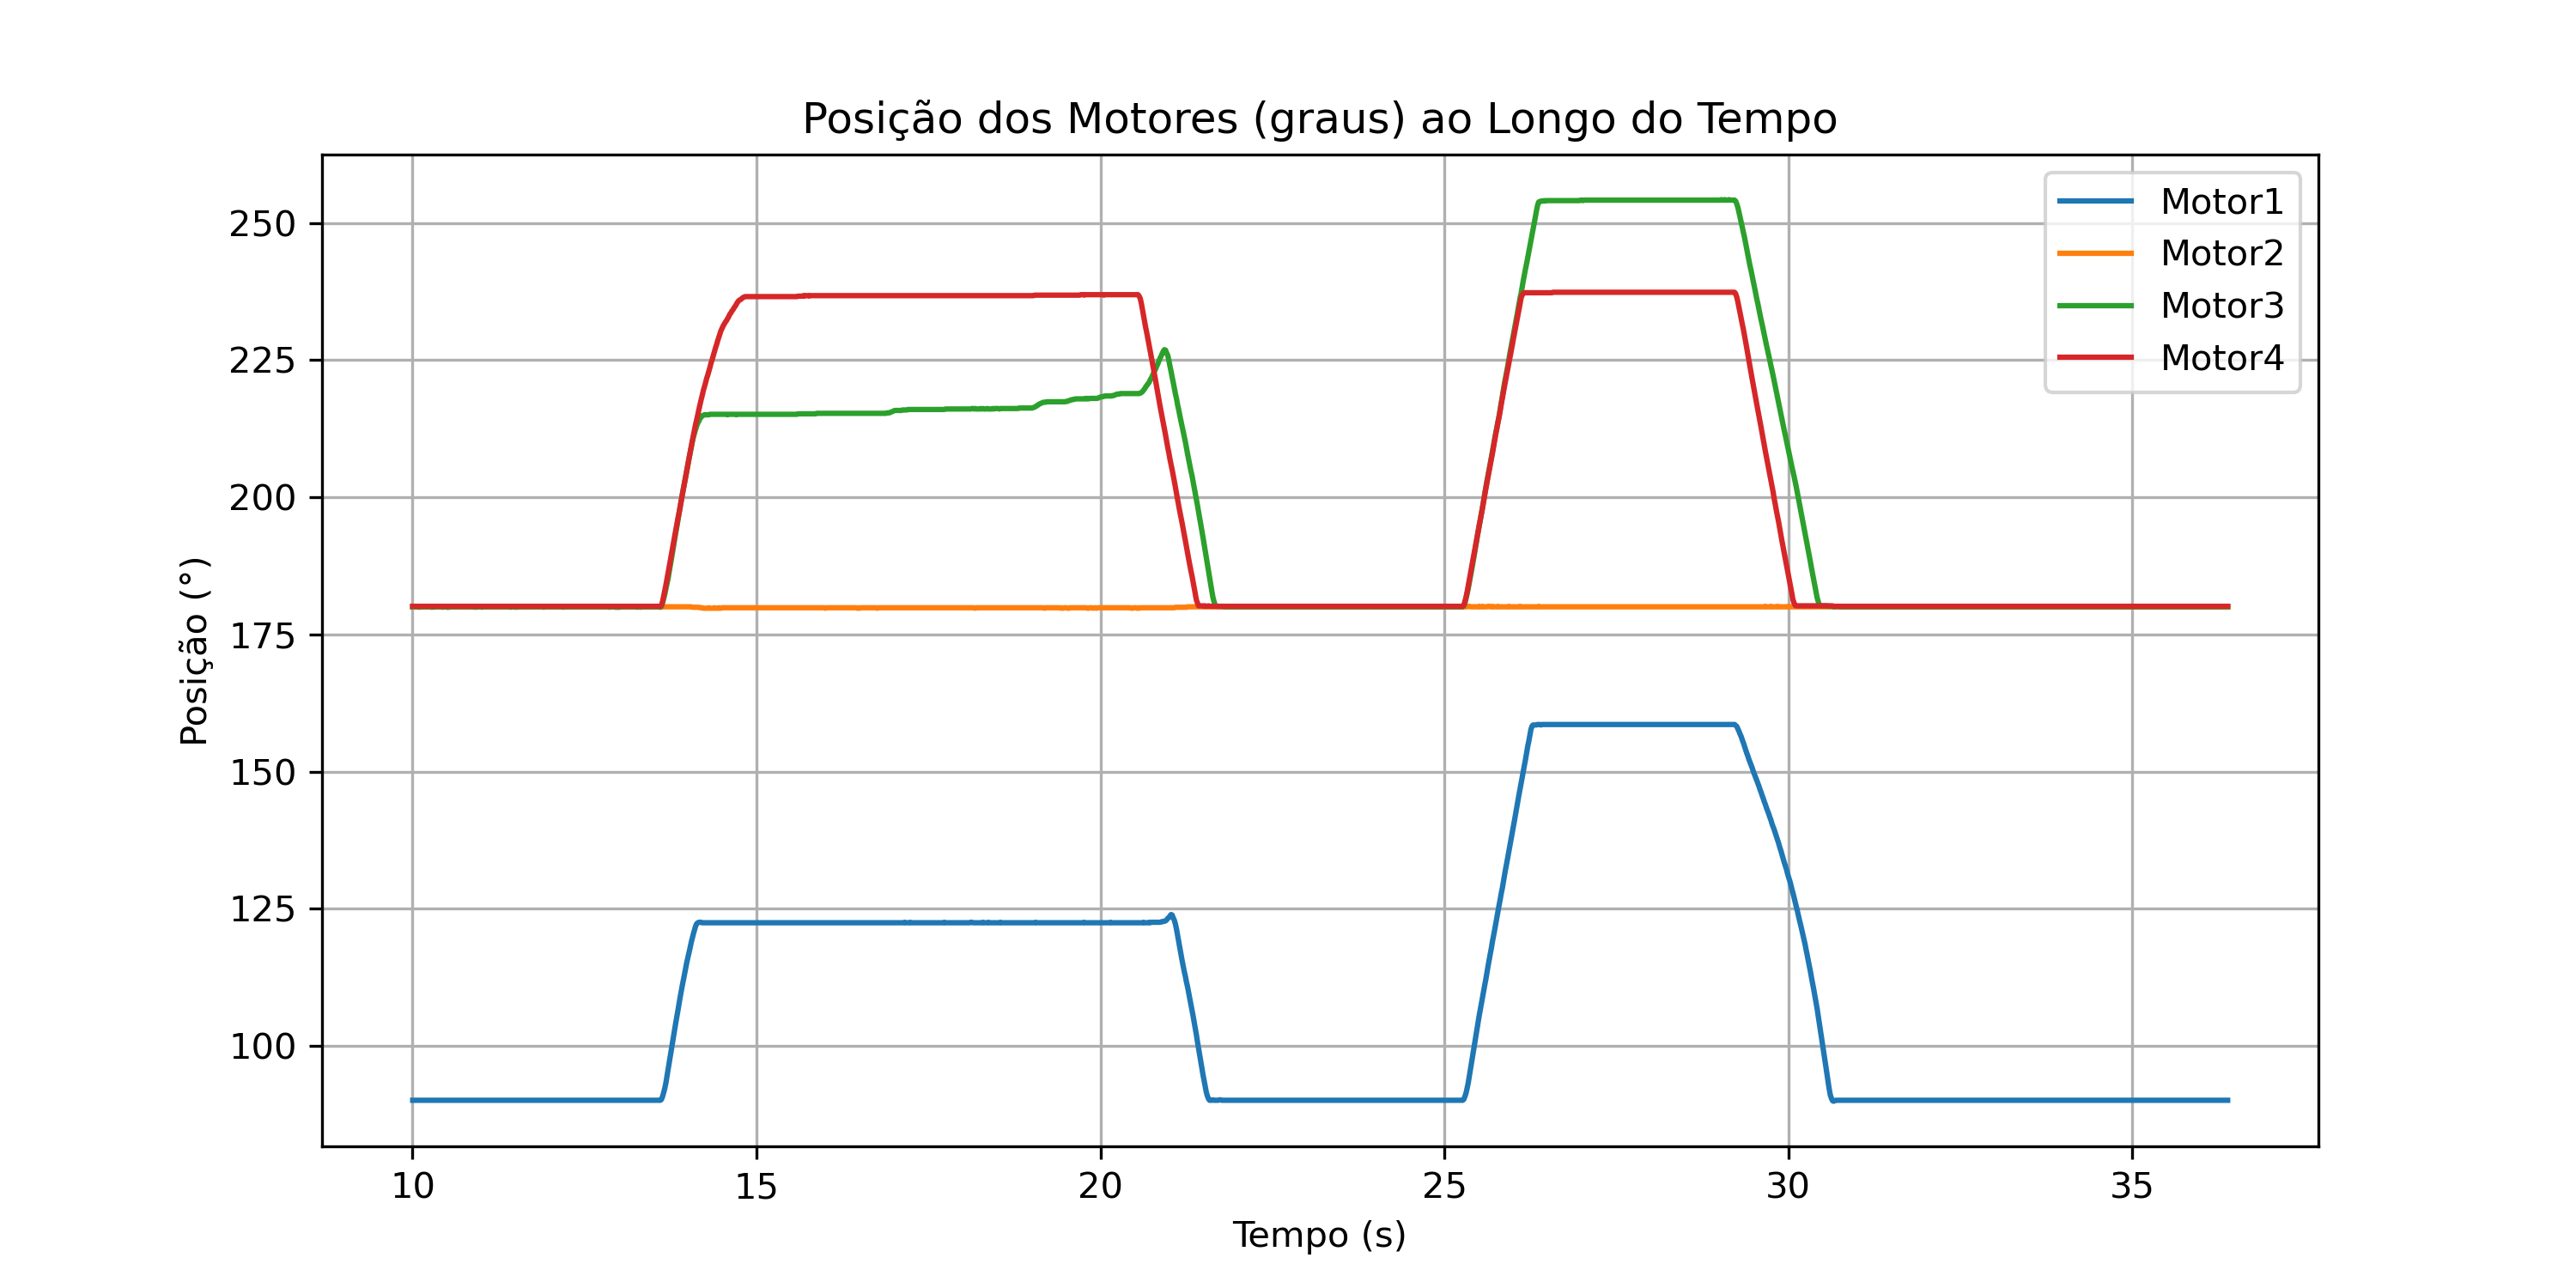
\includegraphics[height=6cm]{figs/chapter4/finger_positions_1.png}
    \caption{Posições dos motores ao longo do tempo durante o fecho e abertura do dedo com obstáculo}
    \label{fig:pos1}
    
\end{figure}
\begin{figure}[H]
    \centering
    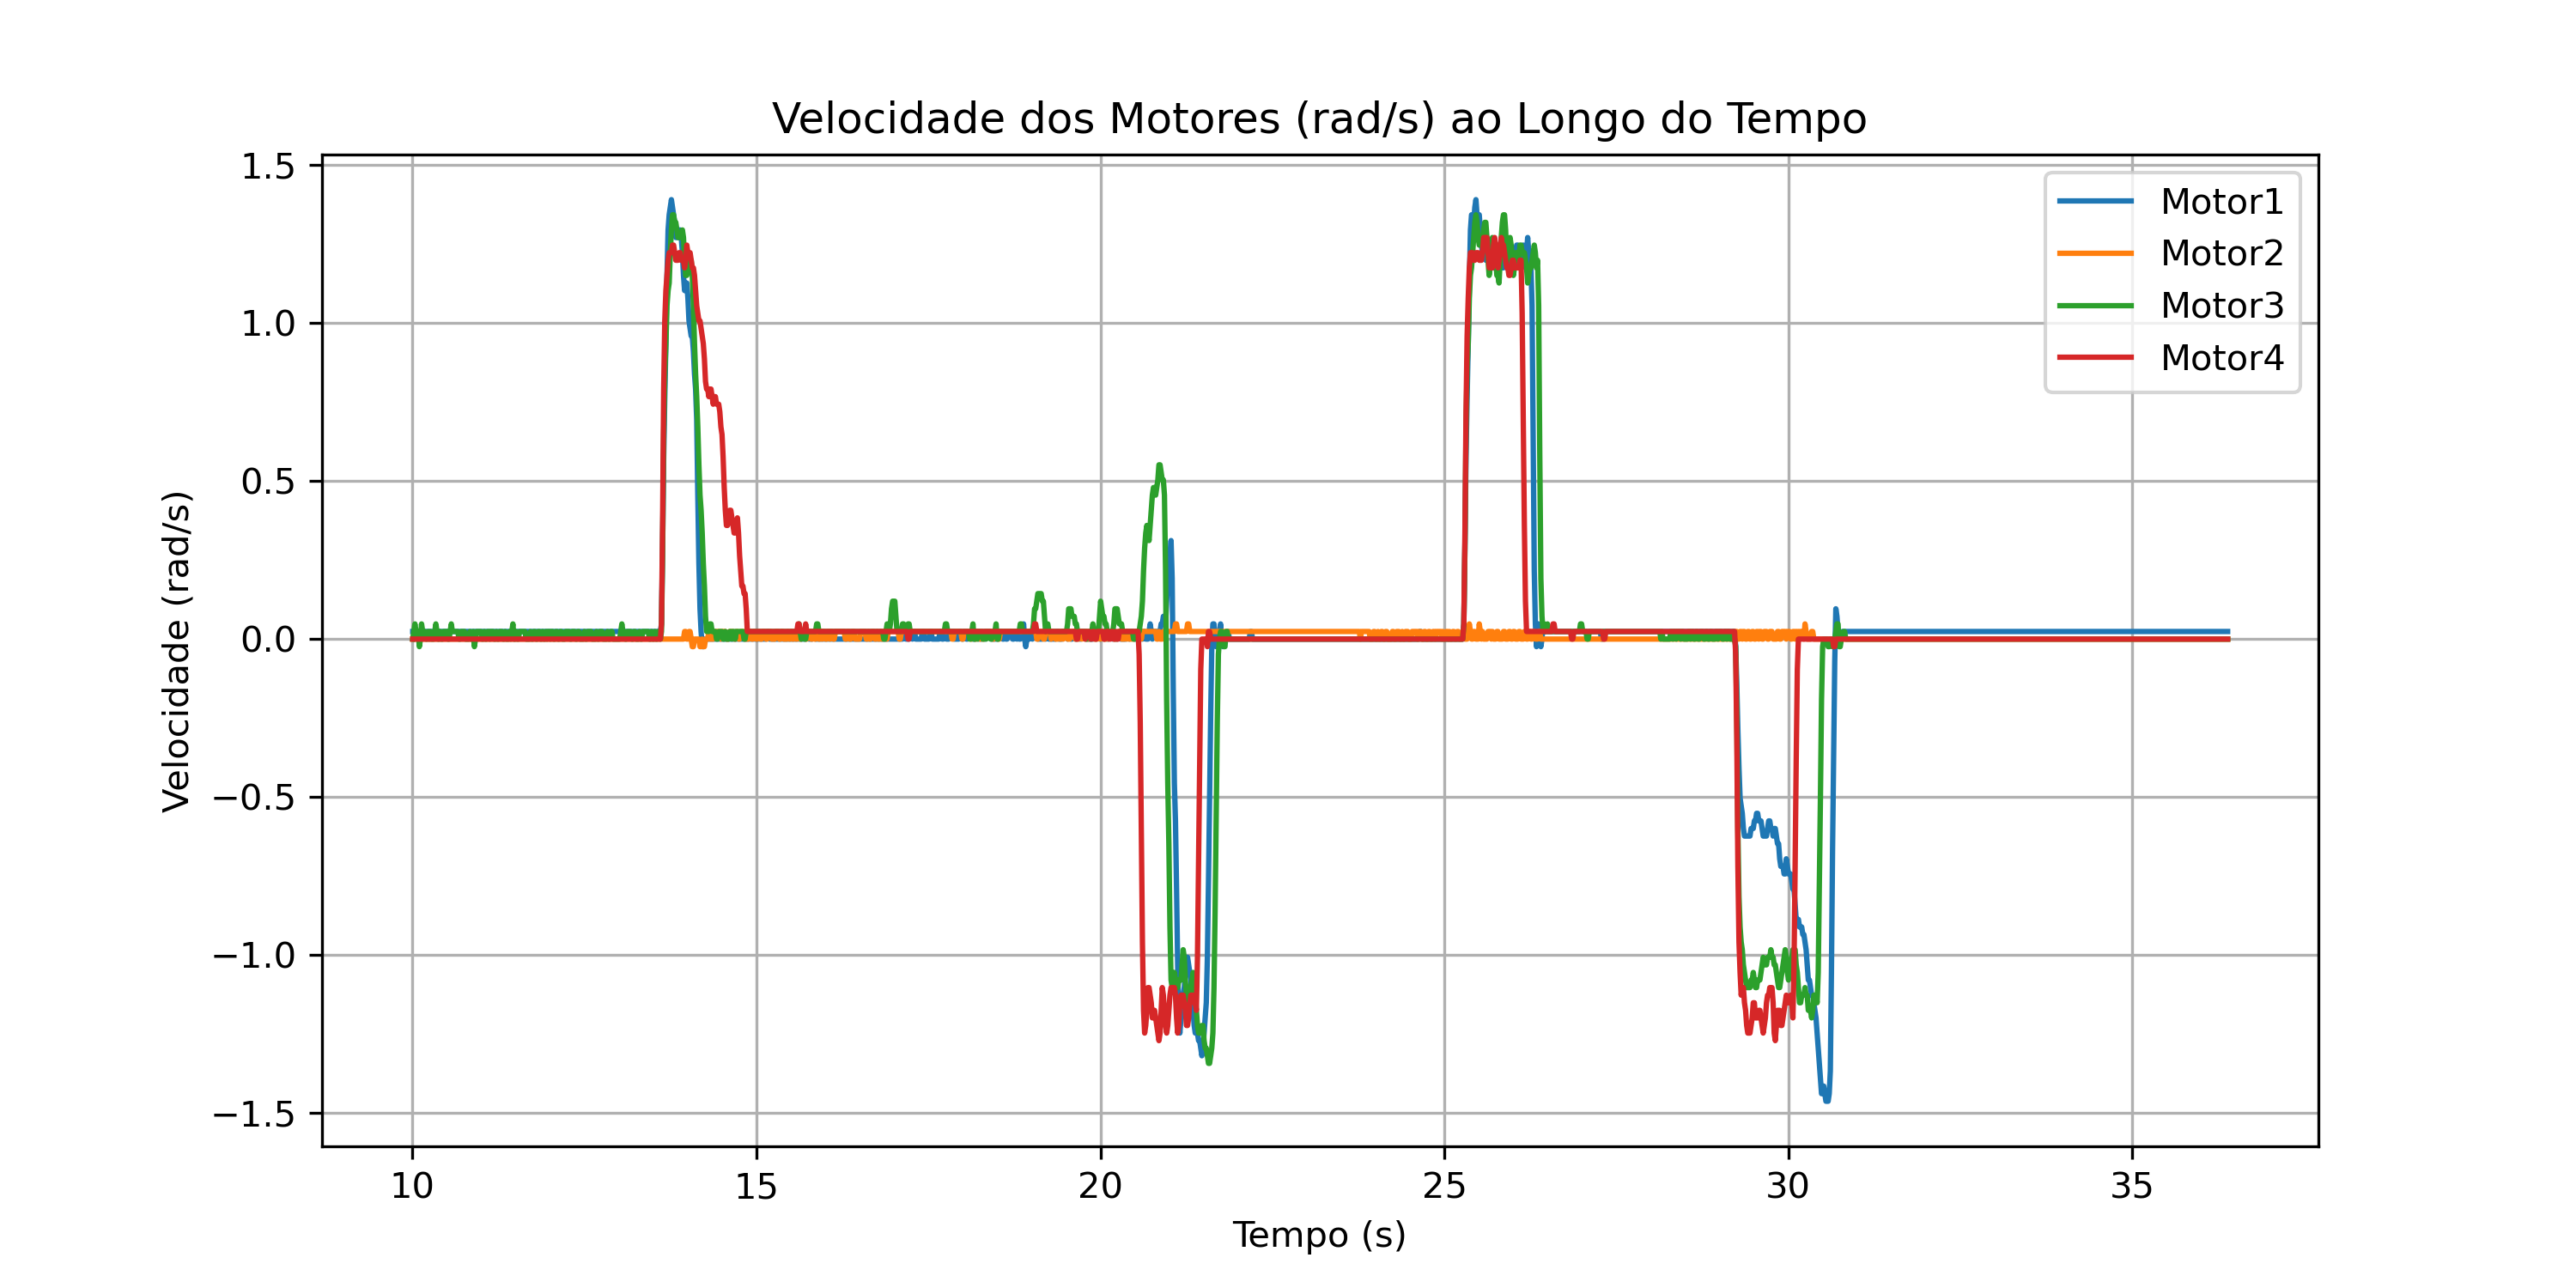
\includegraphics[height=6cm]{figs/chapter4/finger_velocities_1.png}
    \caption{Velocidades dos motores ao longo do tempo durante o fecho e abertura do dedo com obstáculo}
    \label{fig:vels1}
    
\end{figure}
\begin{figure}[H]
    \centering
    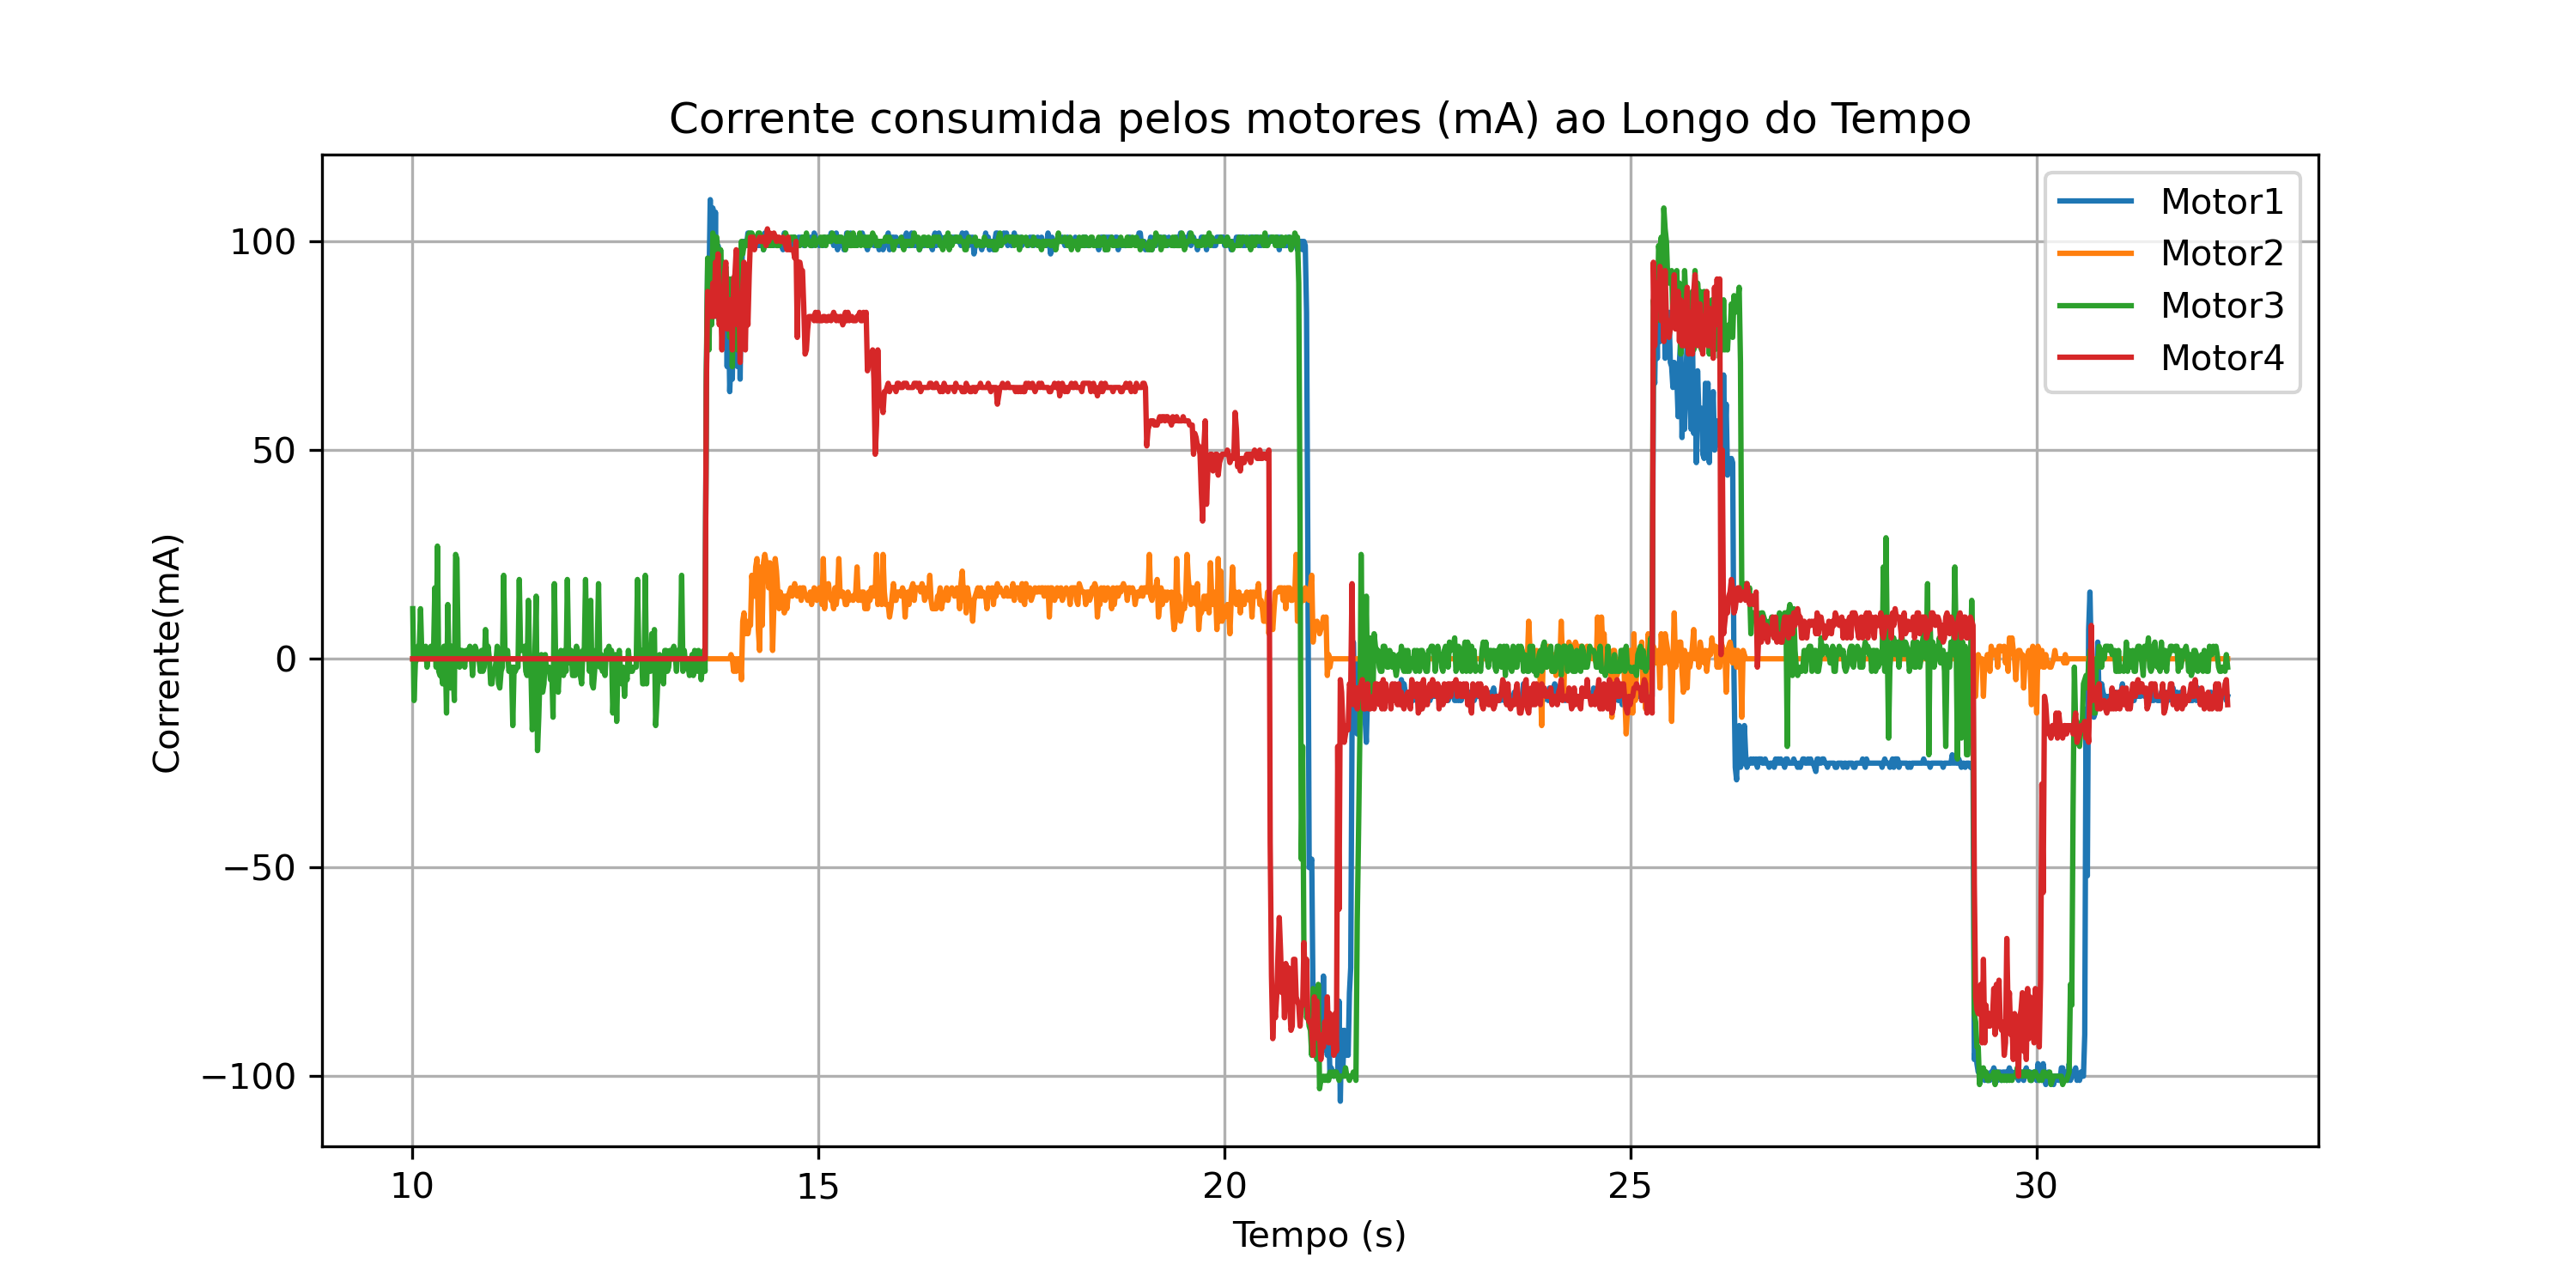
\includegraphics[height=6cm]{figs/chapter4/finger_currents_1.png}
    \caption{Correntes consumidas pelos motores ao longo do tempo durante o fecho e abertura do dedo com obstáculo}
    \label{fig:currs1}
    
\end{figure}

Na presença do obstáculo, o dedo não consegue atingir a posição alvo, resultando numa estabilização precoce da posição e no corte da velocidade. Simultaneamente, verifica-se um aumento significativo na corrente consumida, evidenciando o esforço do motor perante a resistência sem nunca ultrapassar o limite de corrente definido. Após a remoção do obstáculo, o sistema retoma o movimento normal, alcançando a posição desejada com maior estabilidade e menor consumo energético.

Estes resultados comprovam a utilidade e a eficácia do \textit{Current-Based Position Control Mode}, permitindo limitar a força exercida pelos motores durante a interação com o ambiente. Esta funcionalidade é fundamental para aplicações em que a segurança e a adaptabilidade ao contacto com objetos são essenciais, como é o caso da manipulação robótica.

Para além das duas experiências iniciais, foram conduzidos testes adicionais com o objetivo de aprofundar a análise do comportamento dos motores em diferentes condições operacionais. Numa dessas experiências, o dedo foi submetido a movimentos de abertura e fecho com diferentes velocidades máximas configuradas. Os resultados, apresentados no Apêndice~\ref{appendix:teste_velocidades}, demonstram que velocidades mais reduzidas conduzem a um menor consumo energético e a uma variação mais suave da posição ao longo do tempo. A inclinação menos acentuada da curva de posição indica um movimento mais progressivo e controlado, confirmando a influência direta da velocidade sobre a dinâmica do sistema.

Outra experiência relevante consistiu em introduzir obstáculos que interrompessem o movimento do dedo em diferentes posições, com o intuito de estudar o efeito da localização do obstáculo no comportamento individual dos motores. Verificou-se que, quando o obstáculo atua sobre a base do dedo (afetando os motores inferiores), apenas o motor bloqueado entra em esforço, enquanto os restantes continuam a tentar atingir as suas posições alvo. Em contraste, quando o obstáculo é colocado na extremidade do dedo, todos os motores são simultaneamente afetados, ficando em esforço e impedidos de completar o movimento. Esta experiência, cujos gráficos se encontram no Apêndice~\ref{appendix:teste_posições_obstaculos}, reforça ainda a eficácia do controlo baseado em corrente, uma vez que a corrente consumida em nenhuma circunstância ultrapassou o limite máximo previamente definido.

Os dados experimentais obtidos encontram-se acompanhados de gráficos e ligações para vídeos demonstrativos no Apêndice~\ref{appendix:teste_velocidades} e ~\ref{appendix:teste_posições_obstaculos}, permitindo uma análise visual clara dos diferentes comportamentos observados. Estas experiências complementares contribuem significativamente para a validação do sistema de controlo implementado, demonstrando não só a sua eficácia em cenários ideais, mas também a sua robustez perante interações físicas imprevistas.







\subsubsection{Programação da Mão completa}



\subsection{Arquitetura de Software Desenvolvida}



\subsection{Funcionalidades Avançadas}

\subsubsection{Ajuste dinâmico de corrente no contacto com objetos}

\subsubsection{Implementação de velocidades relativas entre dedos e falanges}

\subsubsection{Implementação de atrasos temporais programáveis entre movimentos de dedos}




\section{Implementação dos Sensores de Contacto}


\subsection{Seleção do Microcontrolador}







\subsection{Implementação Física do Sistema sensorial}

\subsubsection{Unidade de Aquisição dos sensores}

\subsubsection{Desenho da peça para fixação}

\subsubsection{Desenvolvimento do PCB}


\subsection{Testes com sensores}

\subsubsection{Testes iniciais com sensores FSR}

\subsubsection{Teste com sensor FSR 406}

\subsubsection{Desenho de Peça para propagar a força para o sensor}


\section{Conclusão}

% \include{chapters/chapter5}
% \include{chapters/chapter6}

%%%%%%%%%%%%%%%%%%%%%%%%%%%%%%%%%%%%%%%%%%%%%%%%%%%%%%%
% End of Thesis text 
%%%%%%%%%%%%%%%%%%%%%%%%%%%%%%%%%%%%%%%%%%%%%%%%%%%%%%%

\backmatter

%%%%%%%%%%%%%%%%%%%%%%%%%%%%%%%%%%%%%%%%%%%%%%%%%%%%%%%
% Print all used references
%%%%%%%%%%%%%%%%%%%%%%%%%%%%%%%%%%%%%%%%%%%%%%%%%%%%%%%

\begingroup
\renewcommand{\bibfont}{\footnotesize}
% Redefine References name to Portuguese
% Change if you are using english
\defbibheading{bibliography}[Referências]{
	\chapter{#1}
}
\SingleSpacing
\setlength\bibitemsep{8pt}
\printbibliography[heading=bibliography]
\endgroup


%%%%%%%%%%%%%%%%%%%%%%%%%%%%%%%%%%%%%%%%%%%%%%%%%%%%%%%
% Load appendix
%%%%%%%%%%%%%%%%%%%%%%%%%%%%%%%%%%%%%%%%%%%%%%%%%%%%%%%

\mainmatterWithoutReset
\appendix

\chapter{Apêndice}

\section{Montagem dos Dedos}


\subsection{Montagem do Polegar}
\begin{figure}[H]
\centering
\begin{tabular}{ccc}
  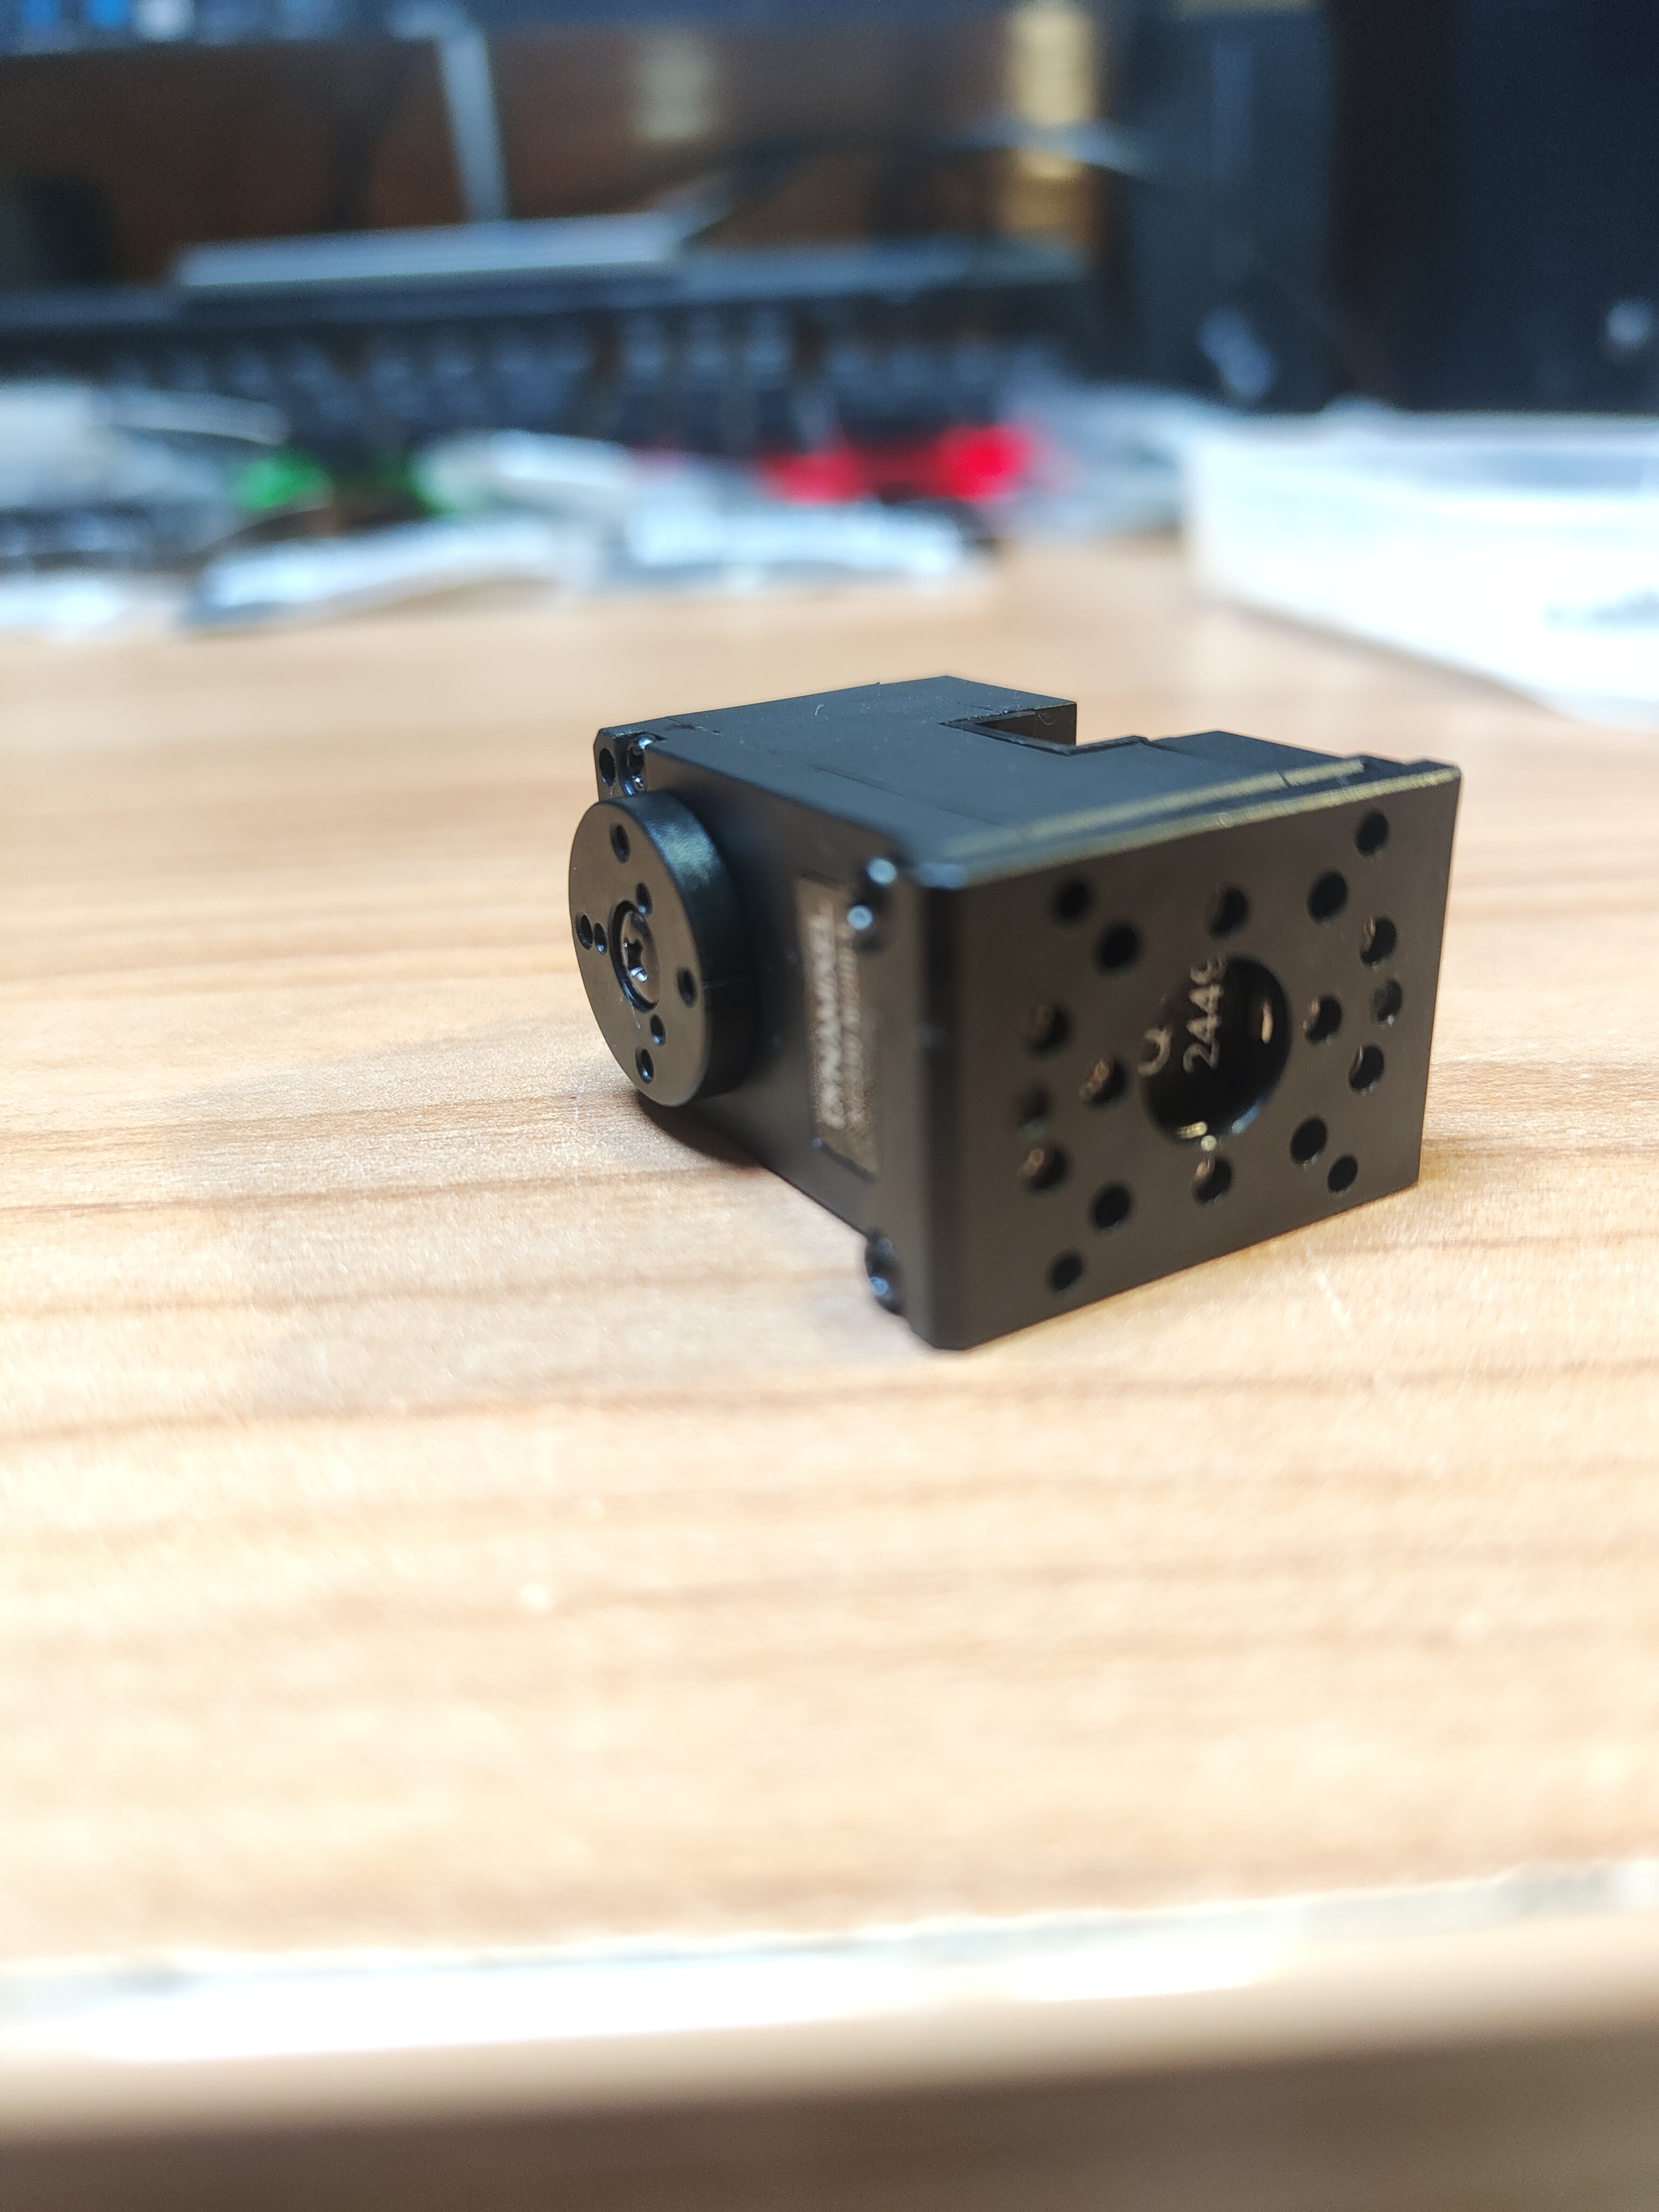
\includegraphics[width=0.25\textwidth]{figs/appendix/polegar/1.jpg} &
  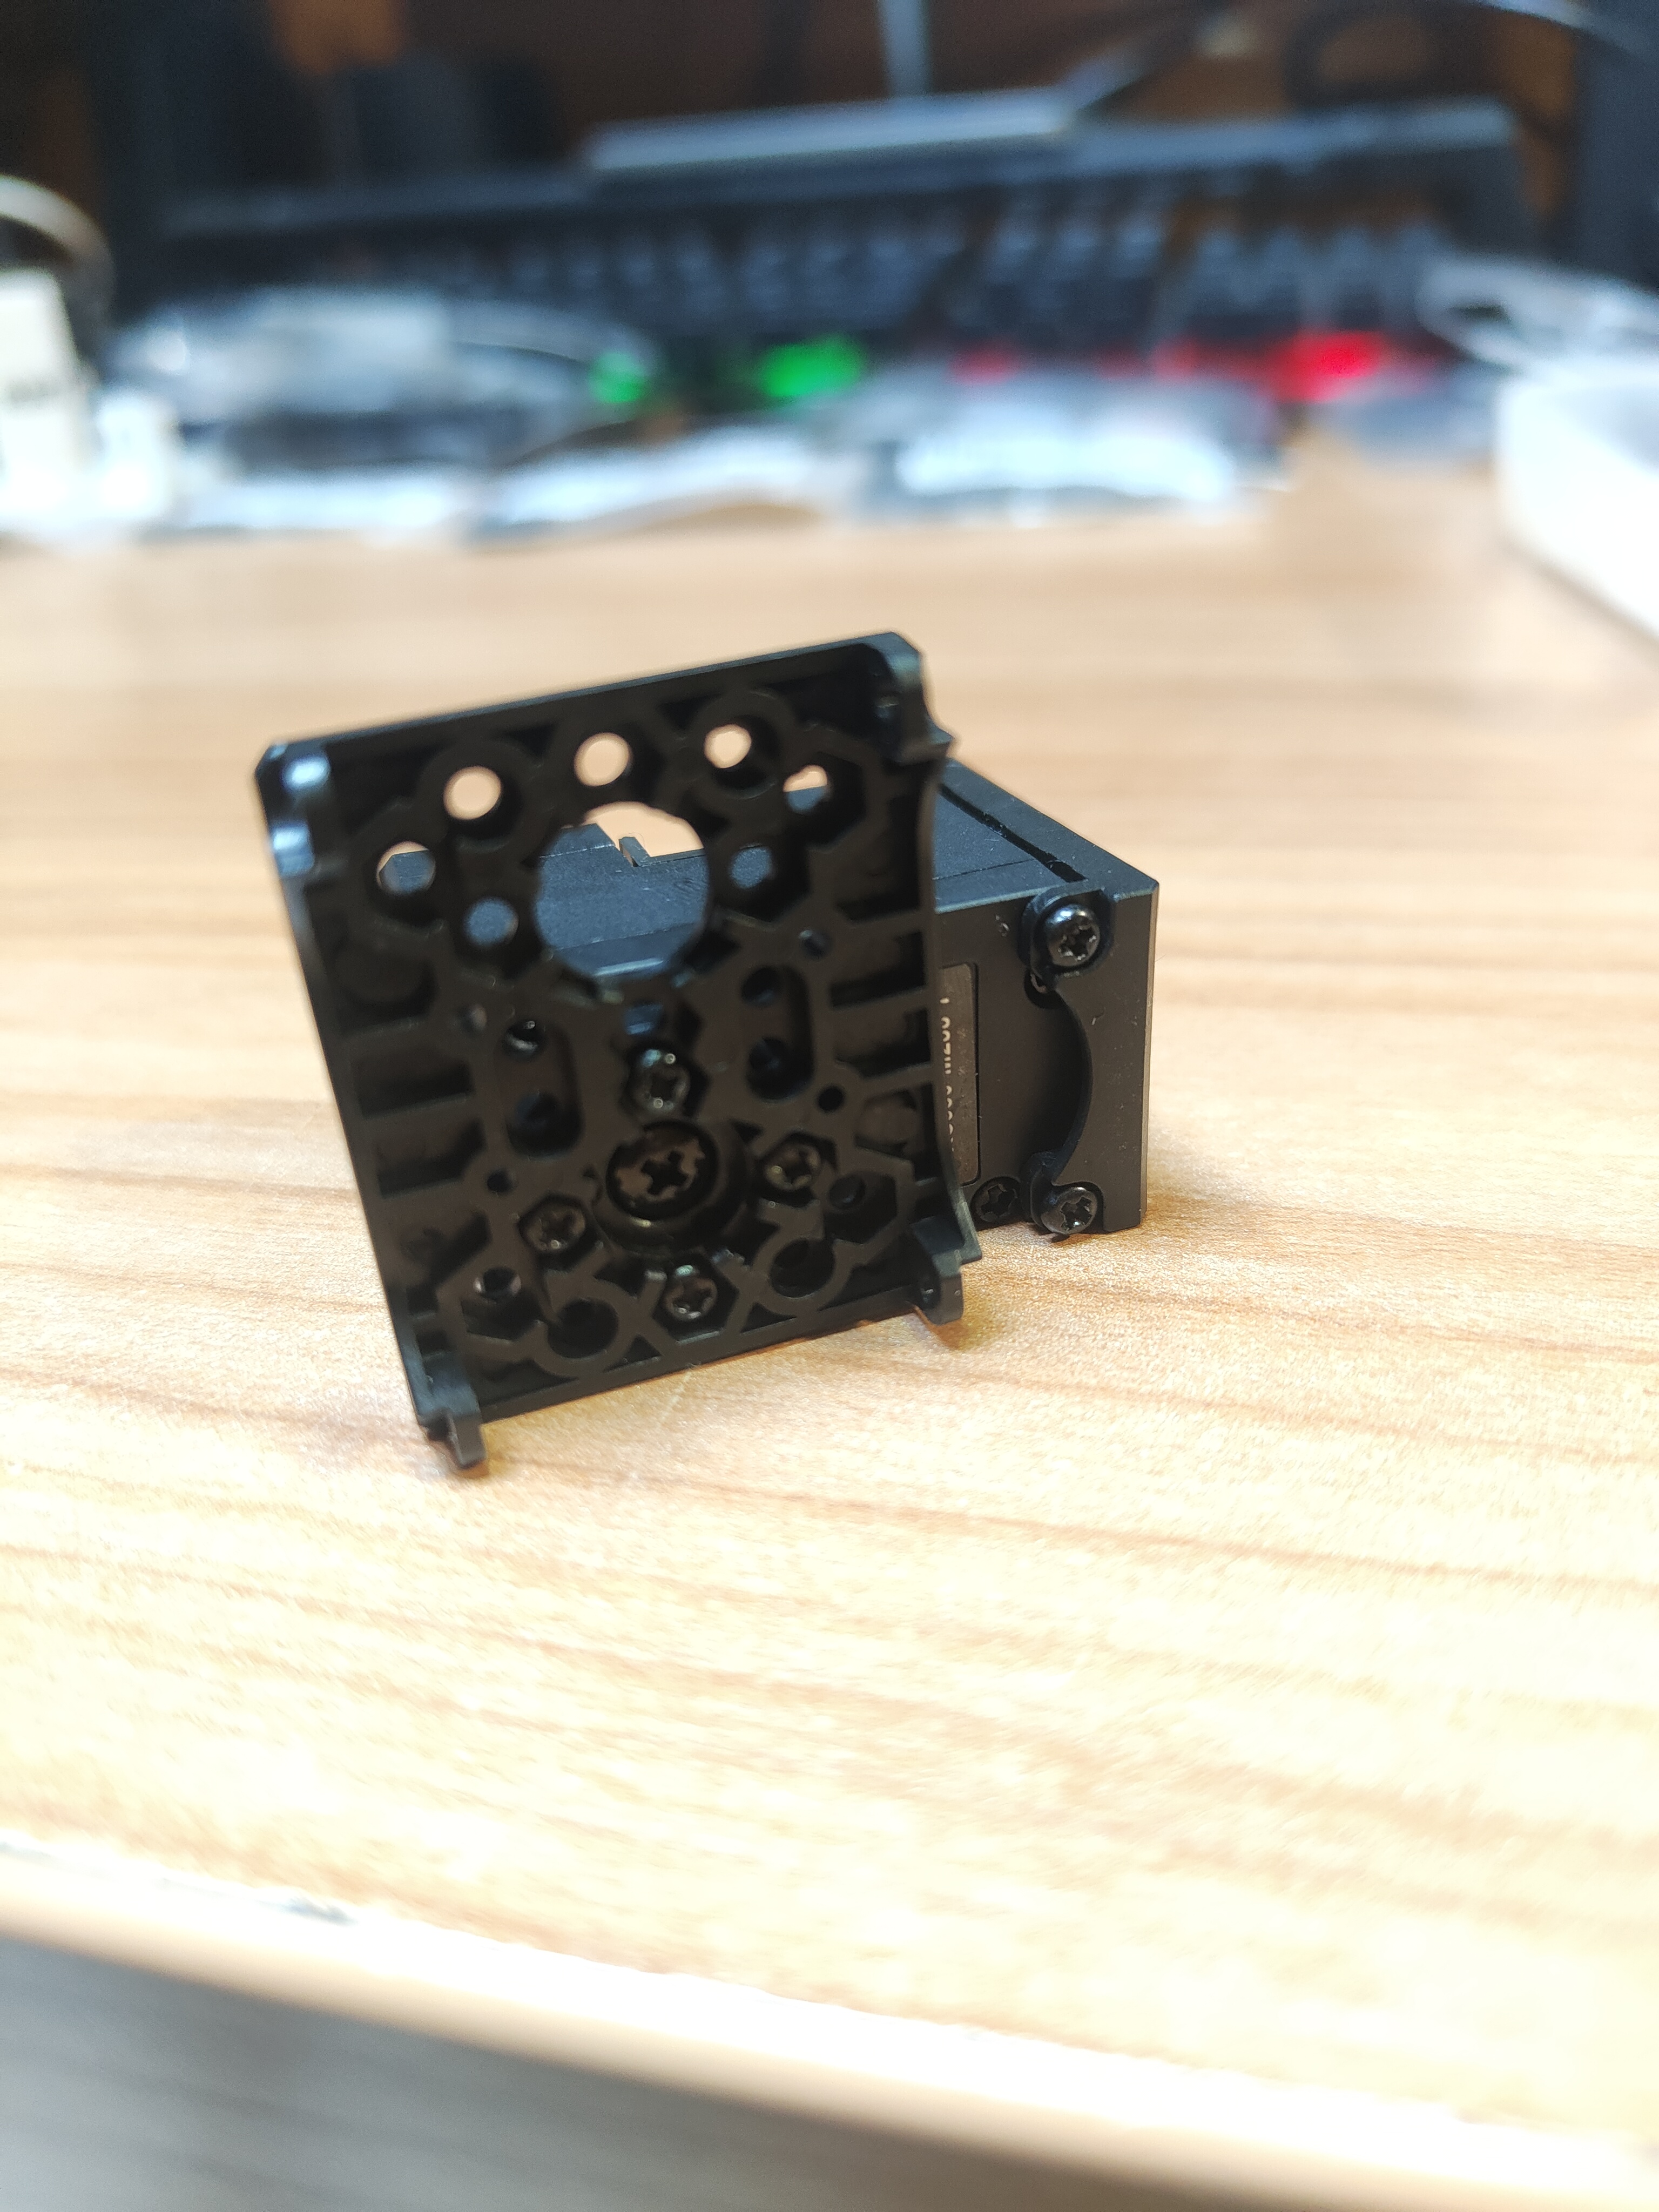
\includegraphics[width=0.25\textwidth]{figs/appendix/polegar/2.jpg} &
  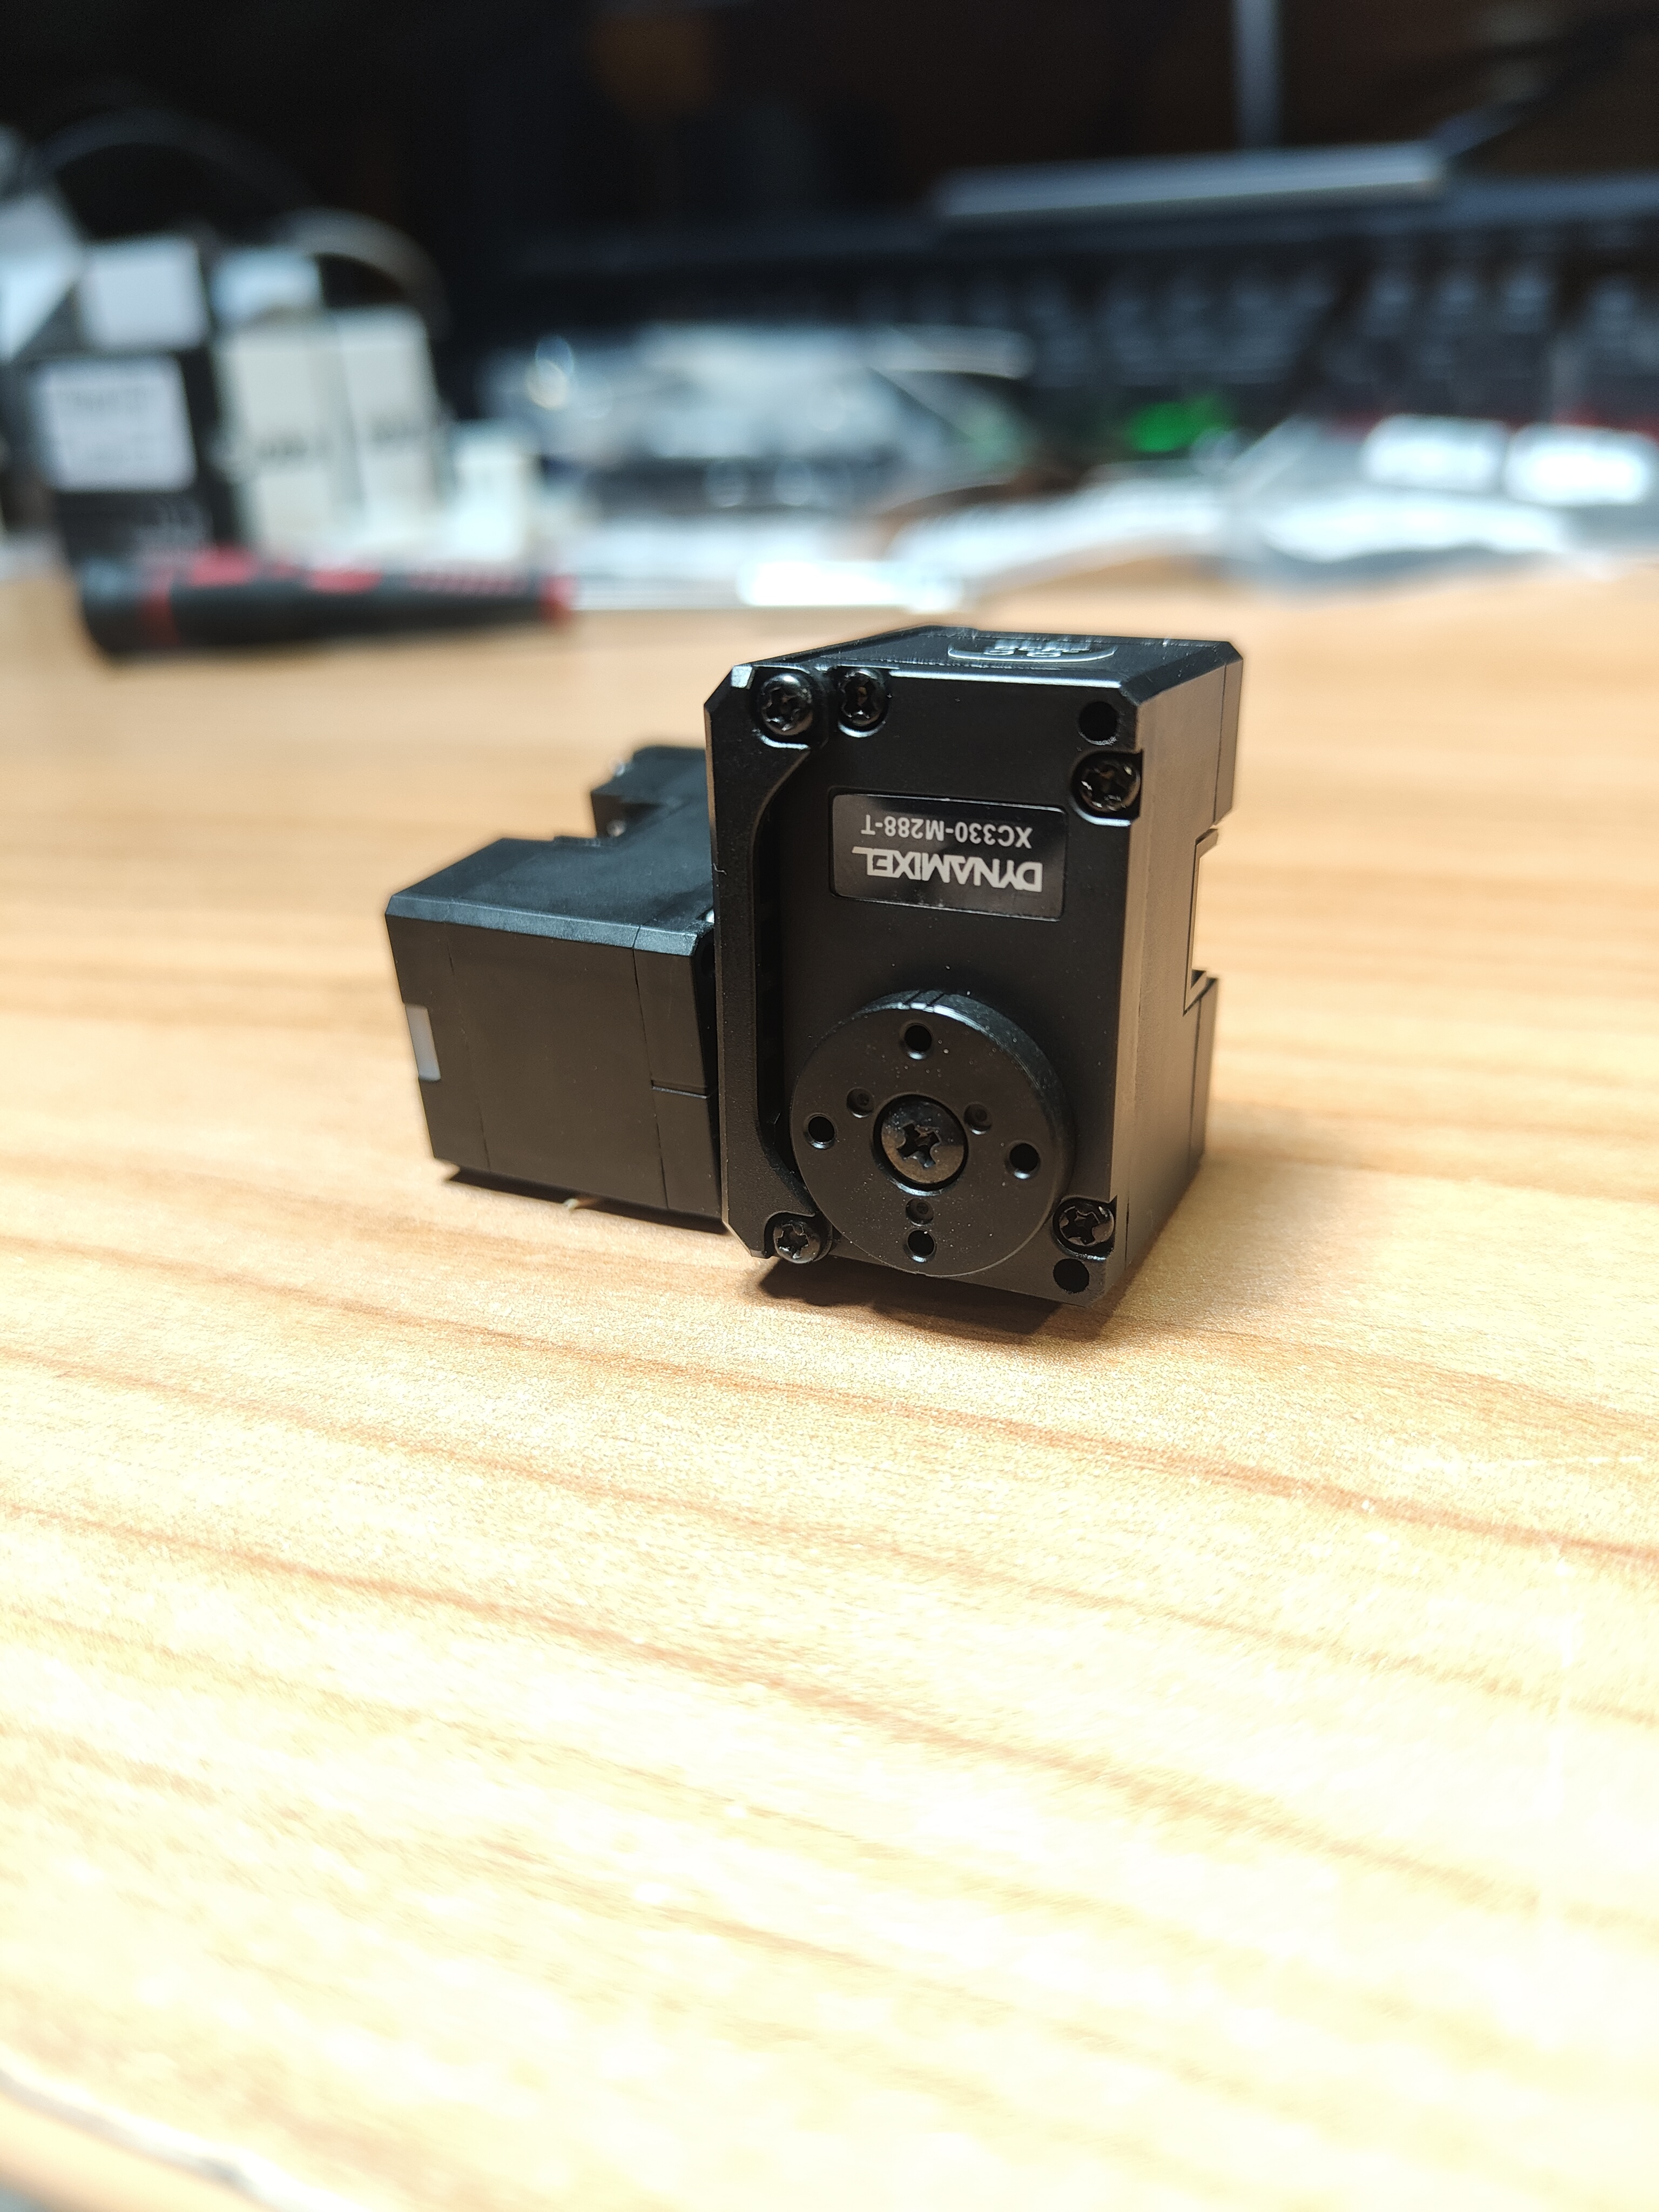
\includegraphics[width=0.25\textwidth]{figs/appendix/polegar/3.jpg} \\
  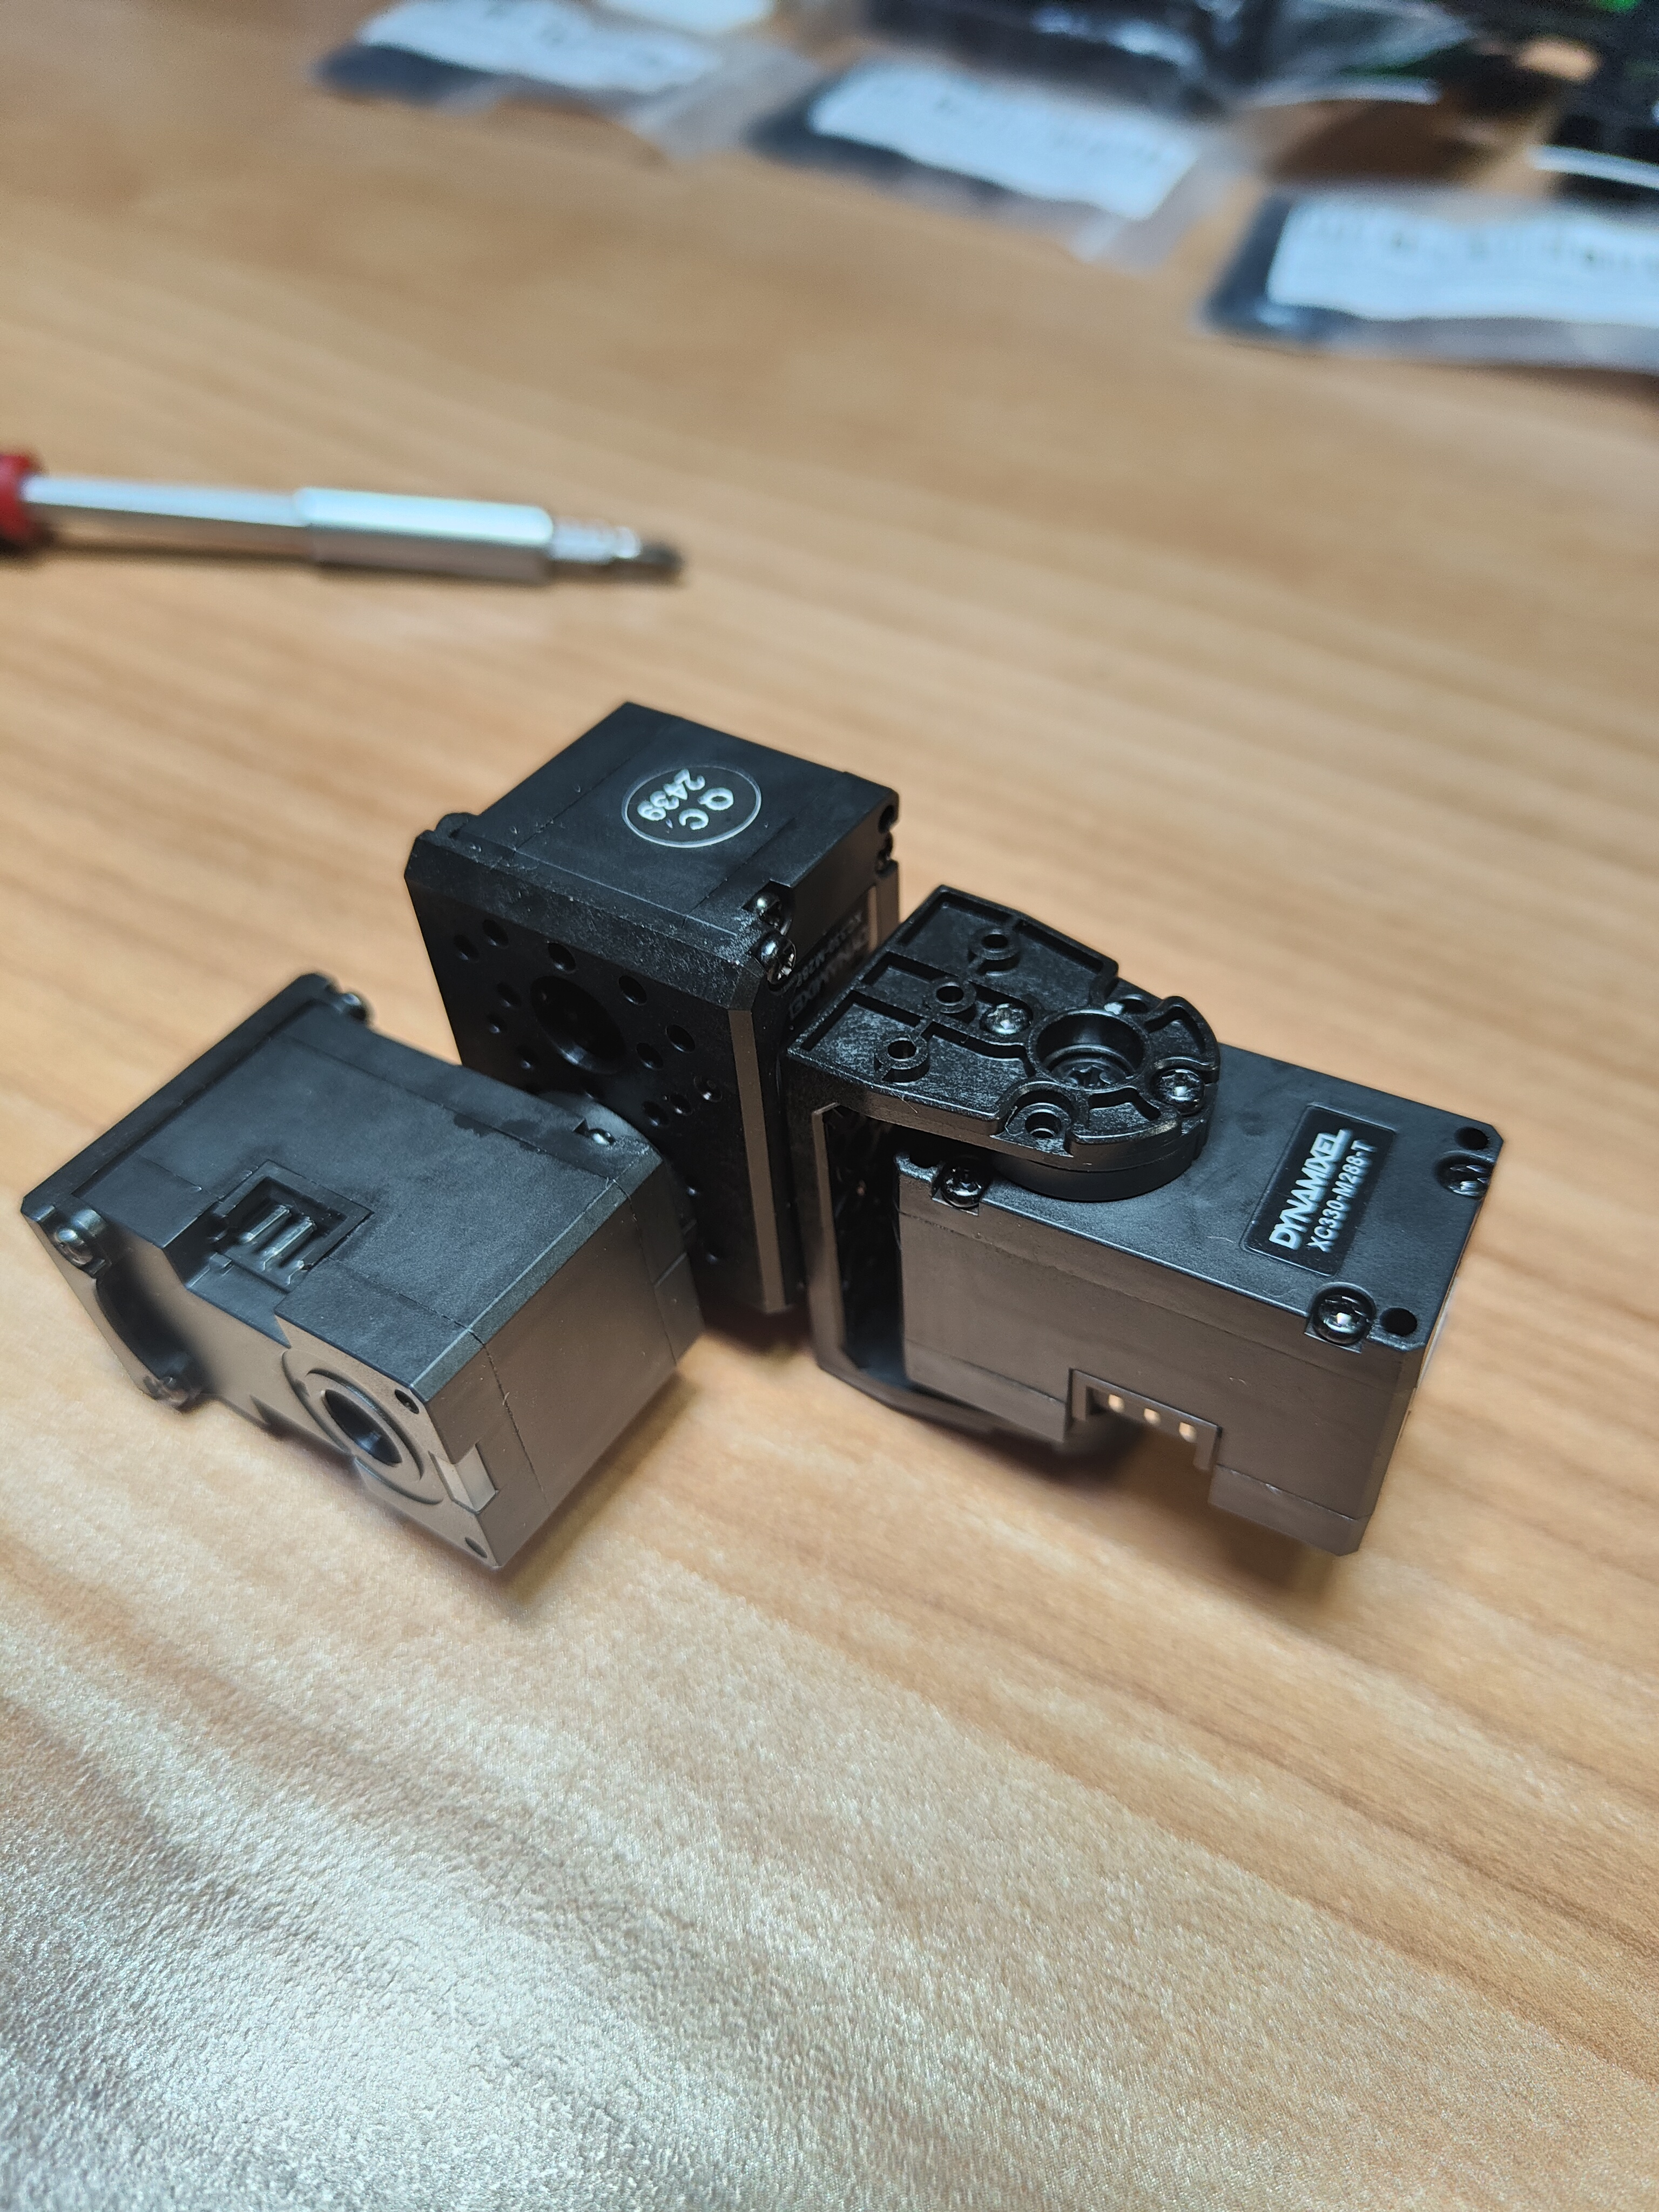
\includegraphics[width=0.25\textwidth]{figs/appendix/polegar/4.jpg} &
  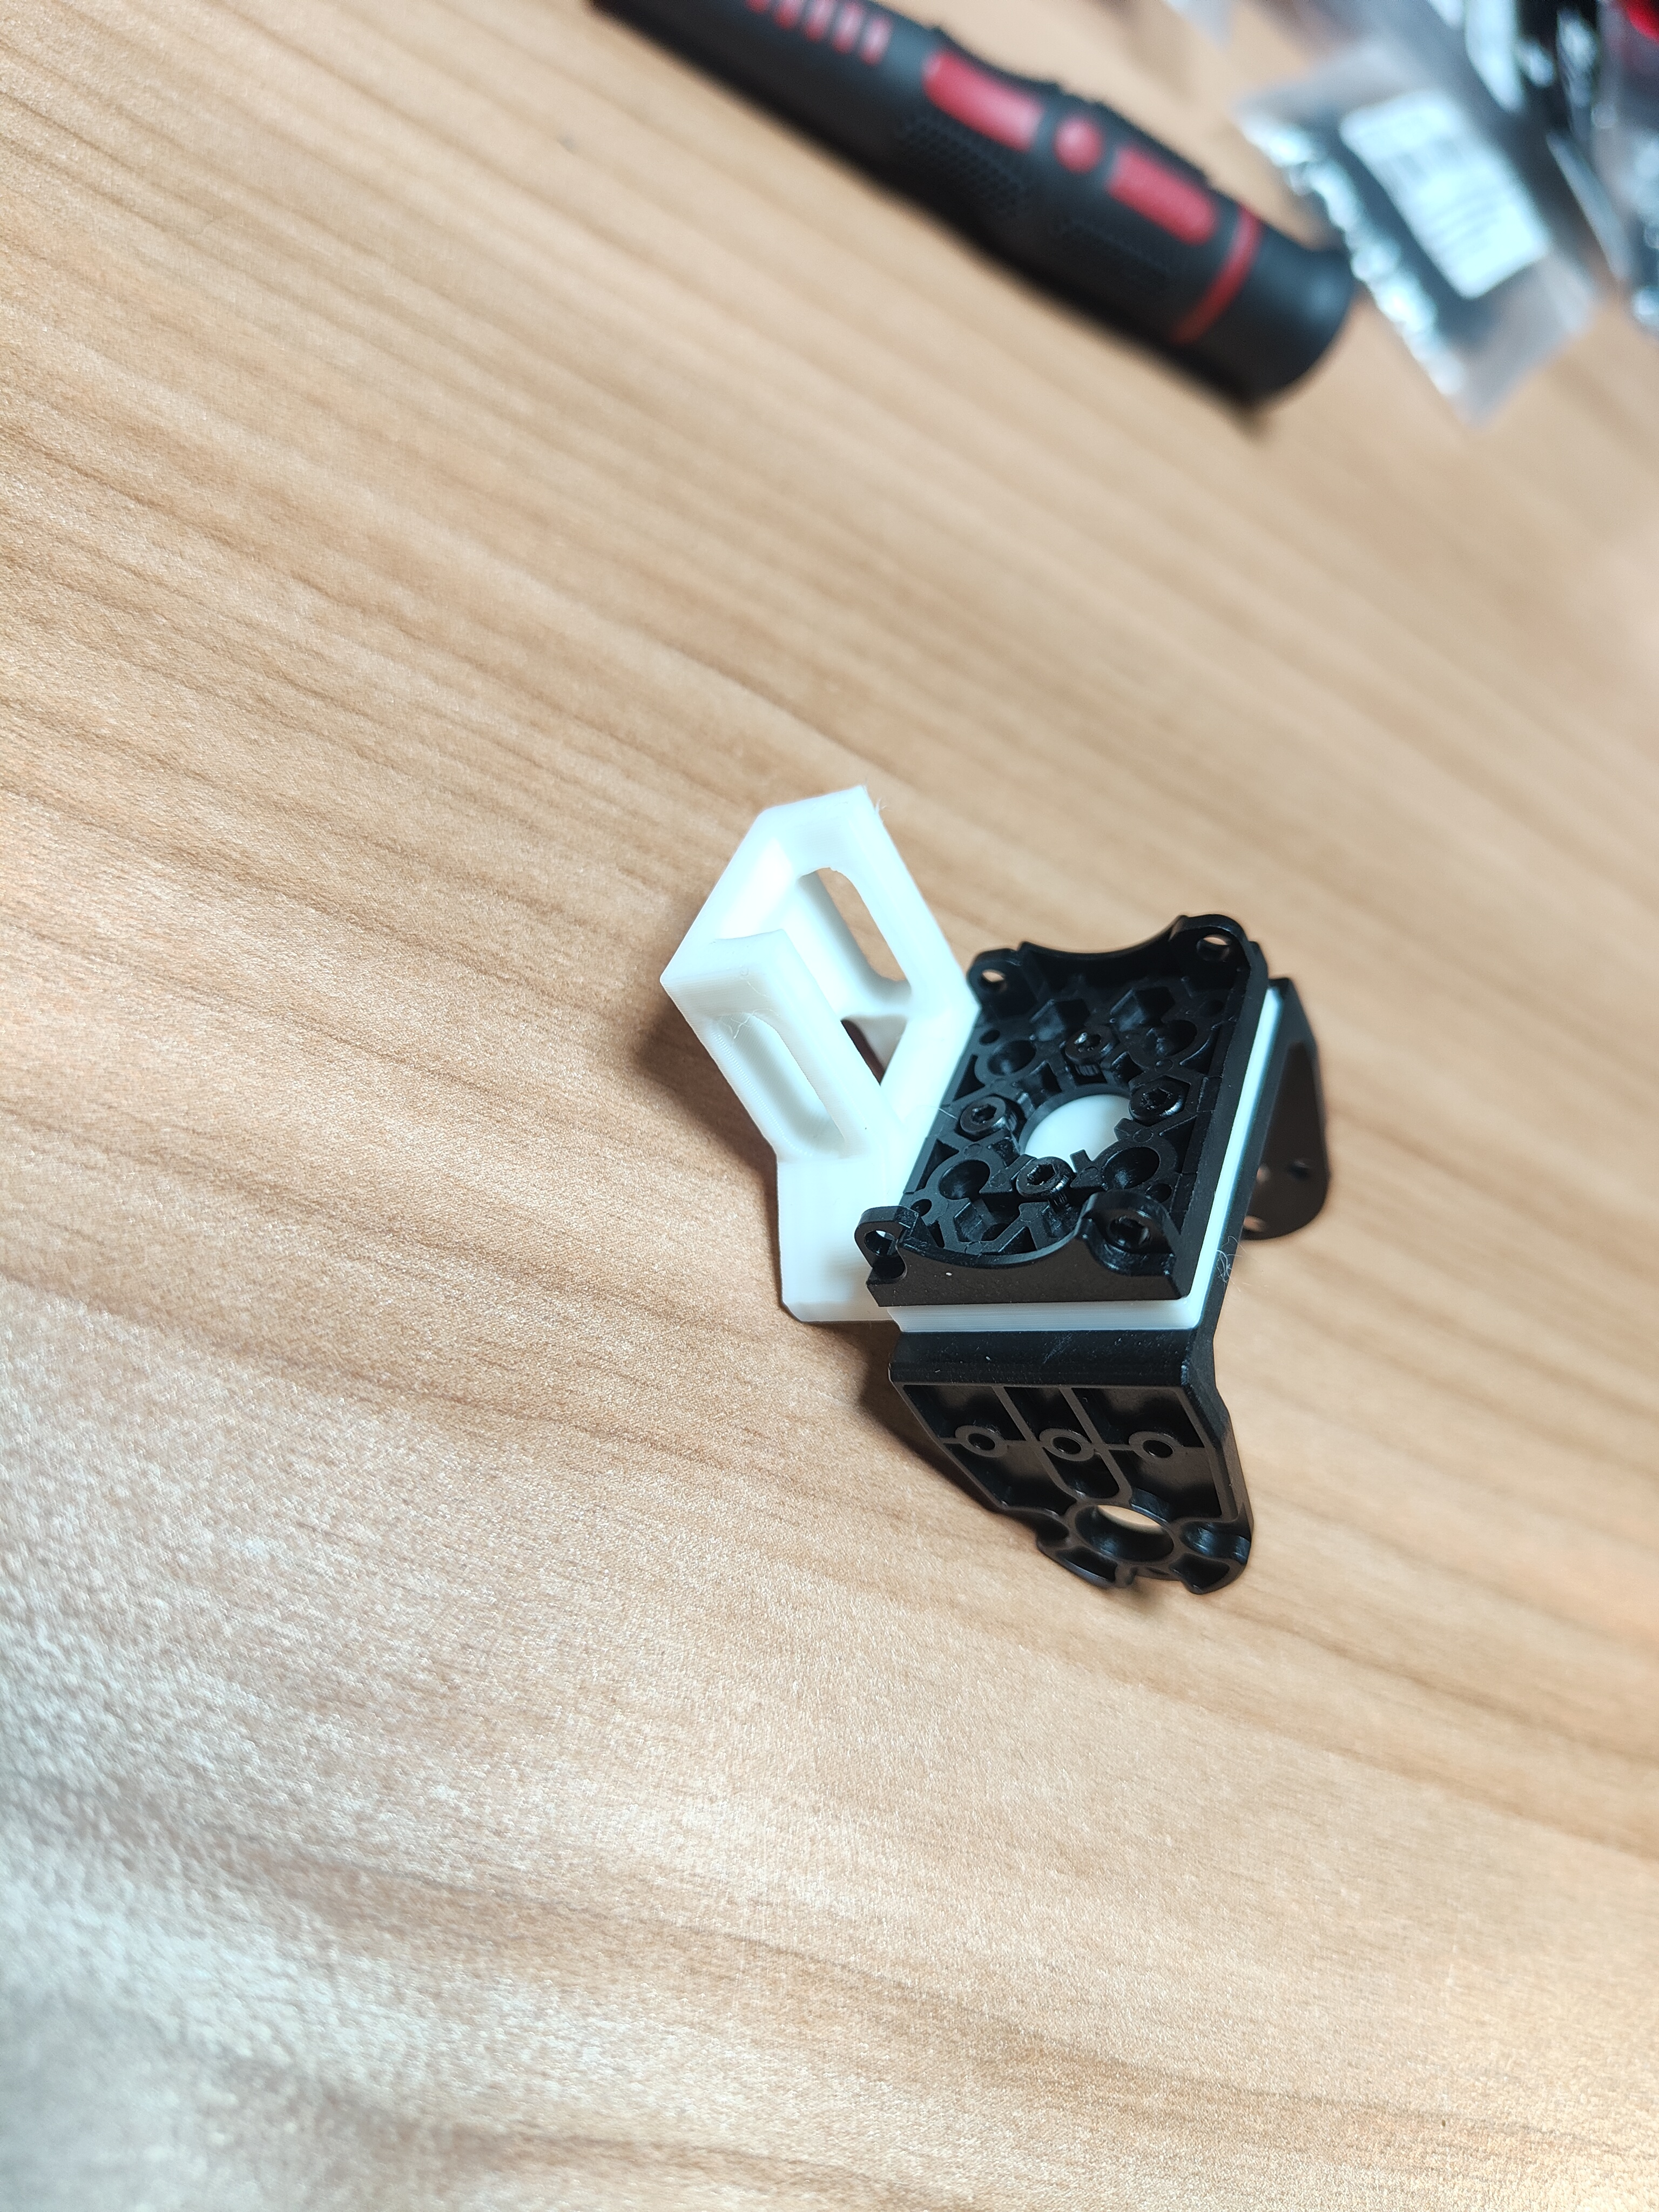
\includegraphics[width=0.25\textwidth]{figs/appendix/polegar/5.jpg} &
  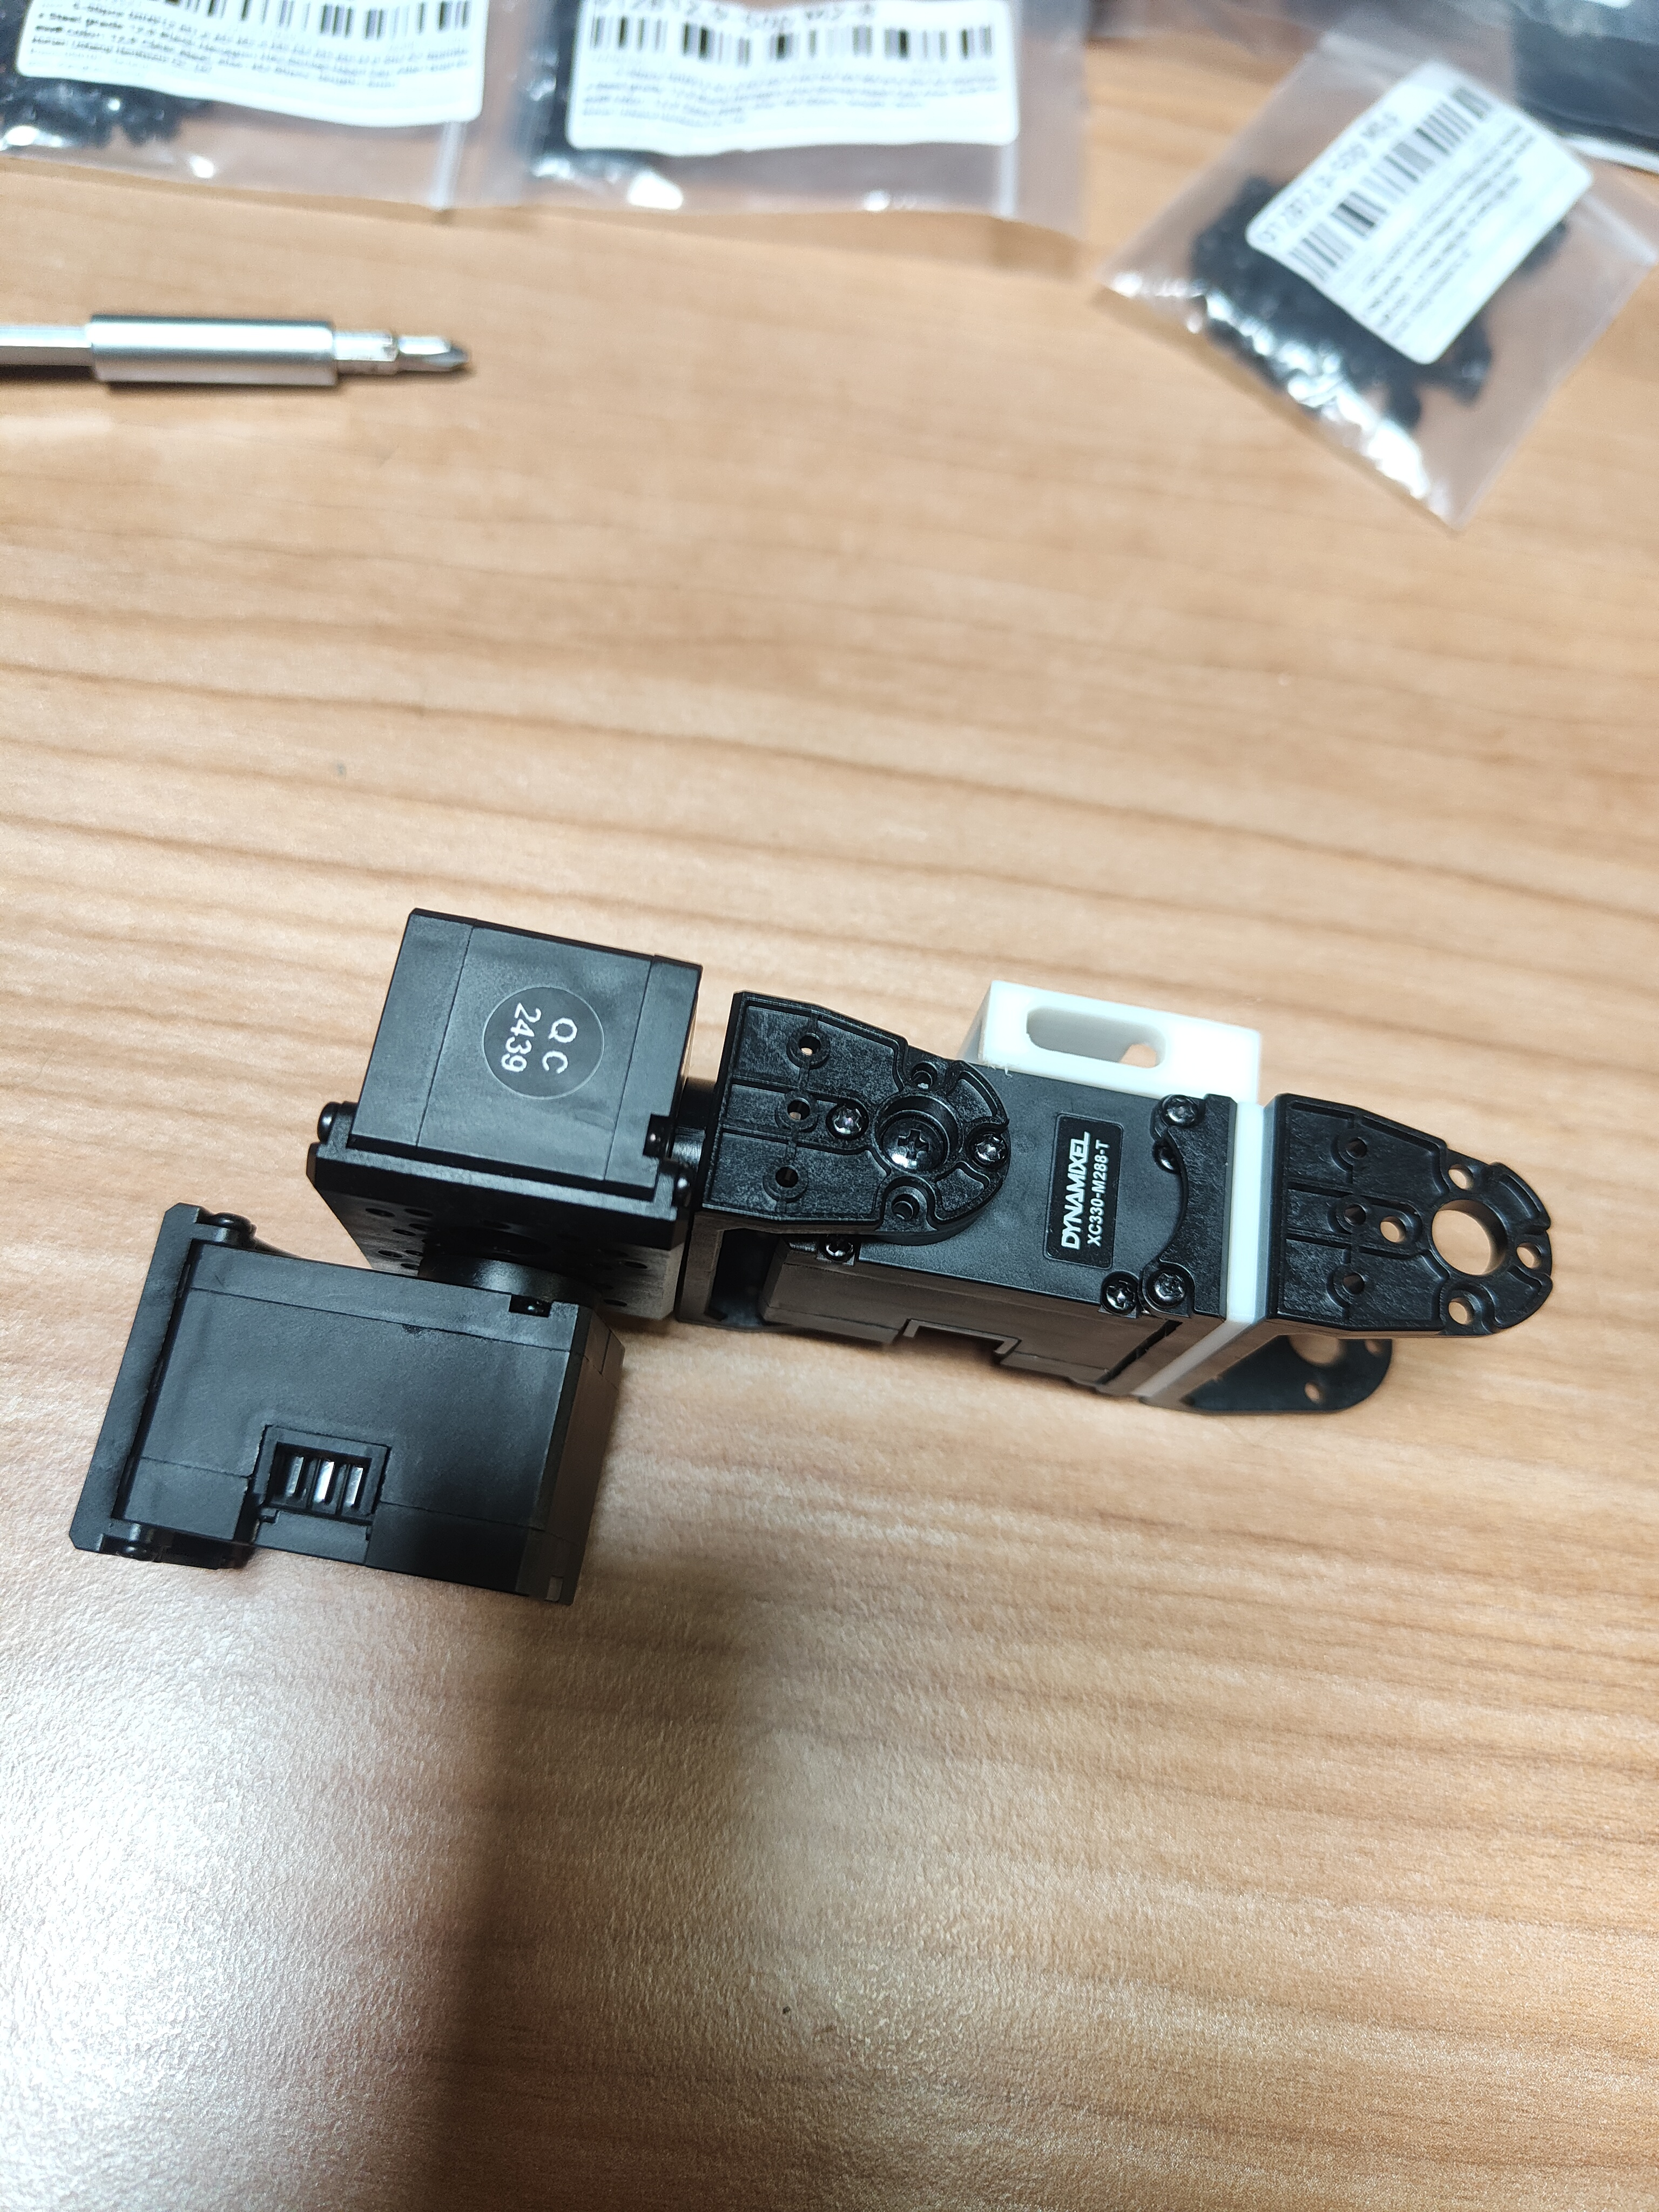
\includegraphics[width=0.25\textwidth]{figs/appendix/polegar/6.jpg} \\
  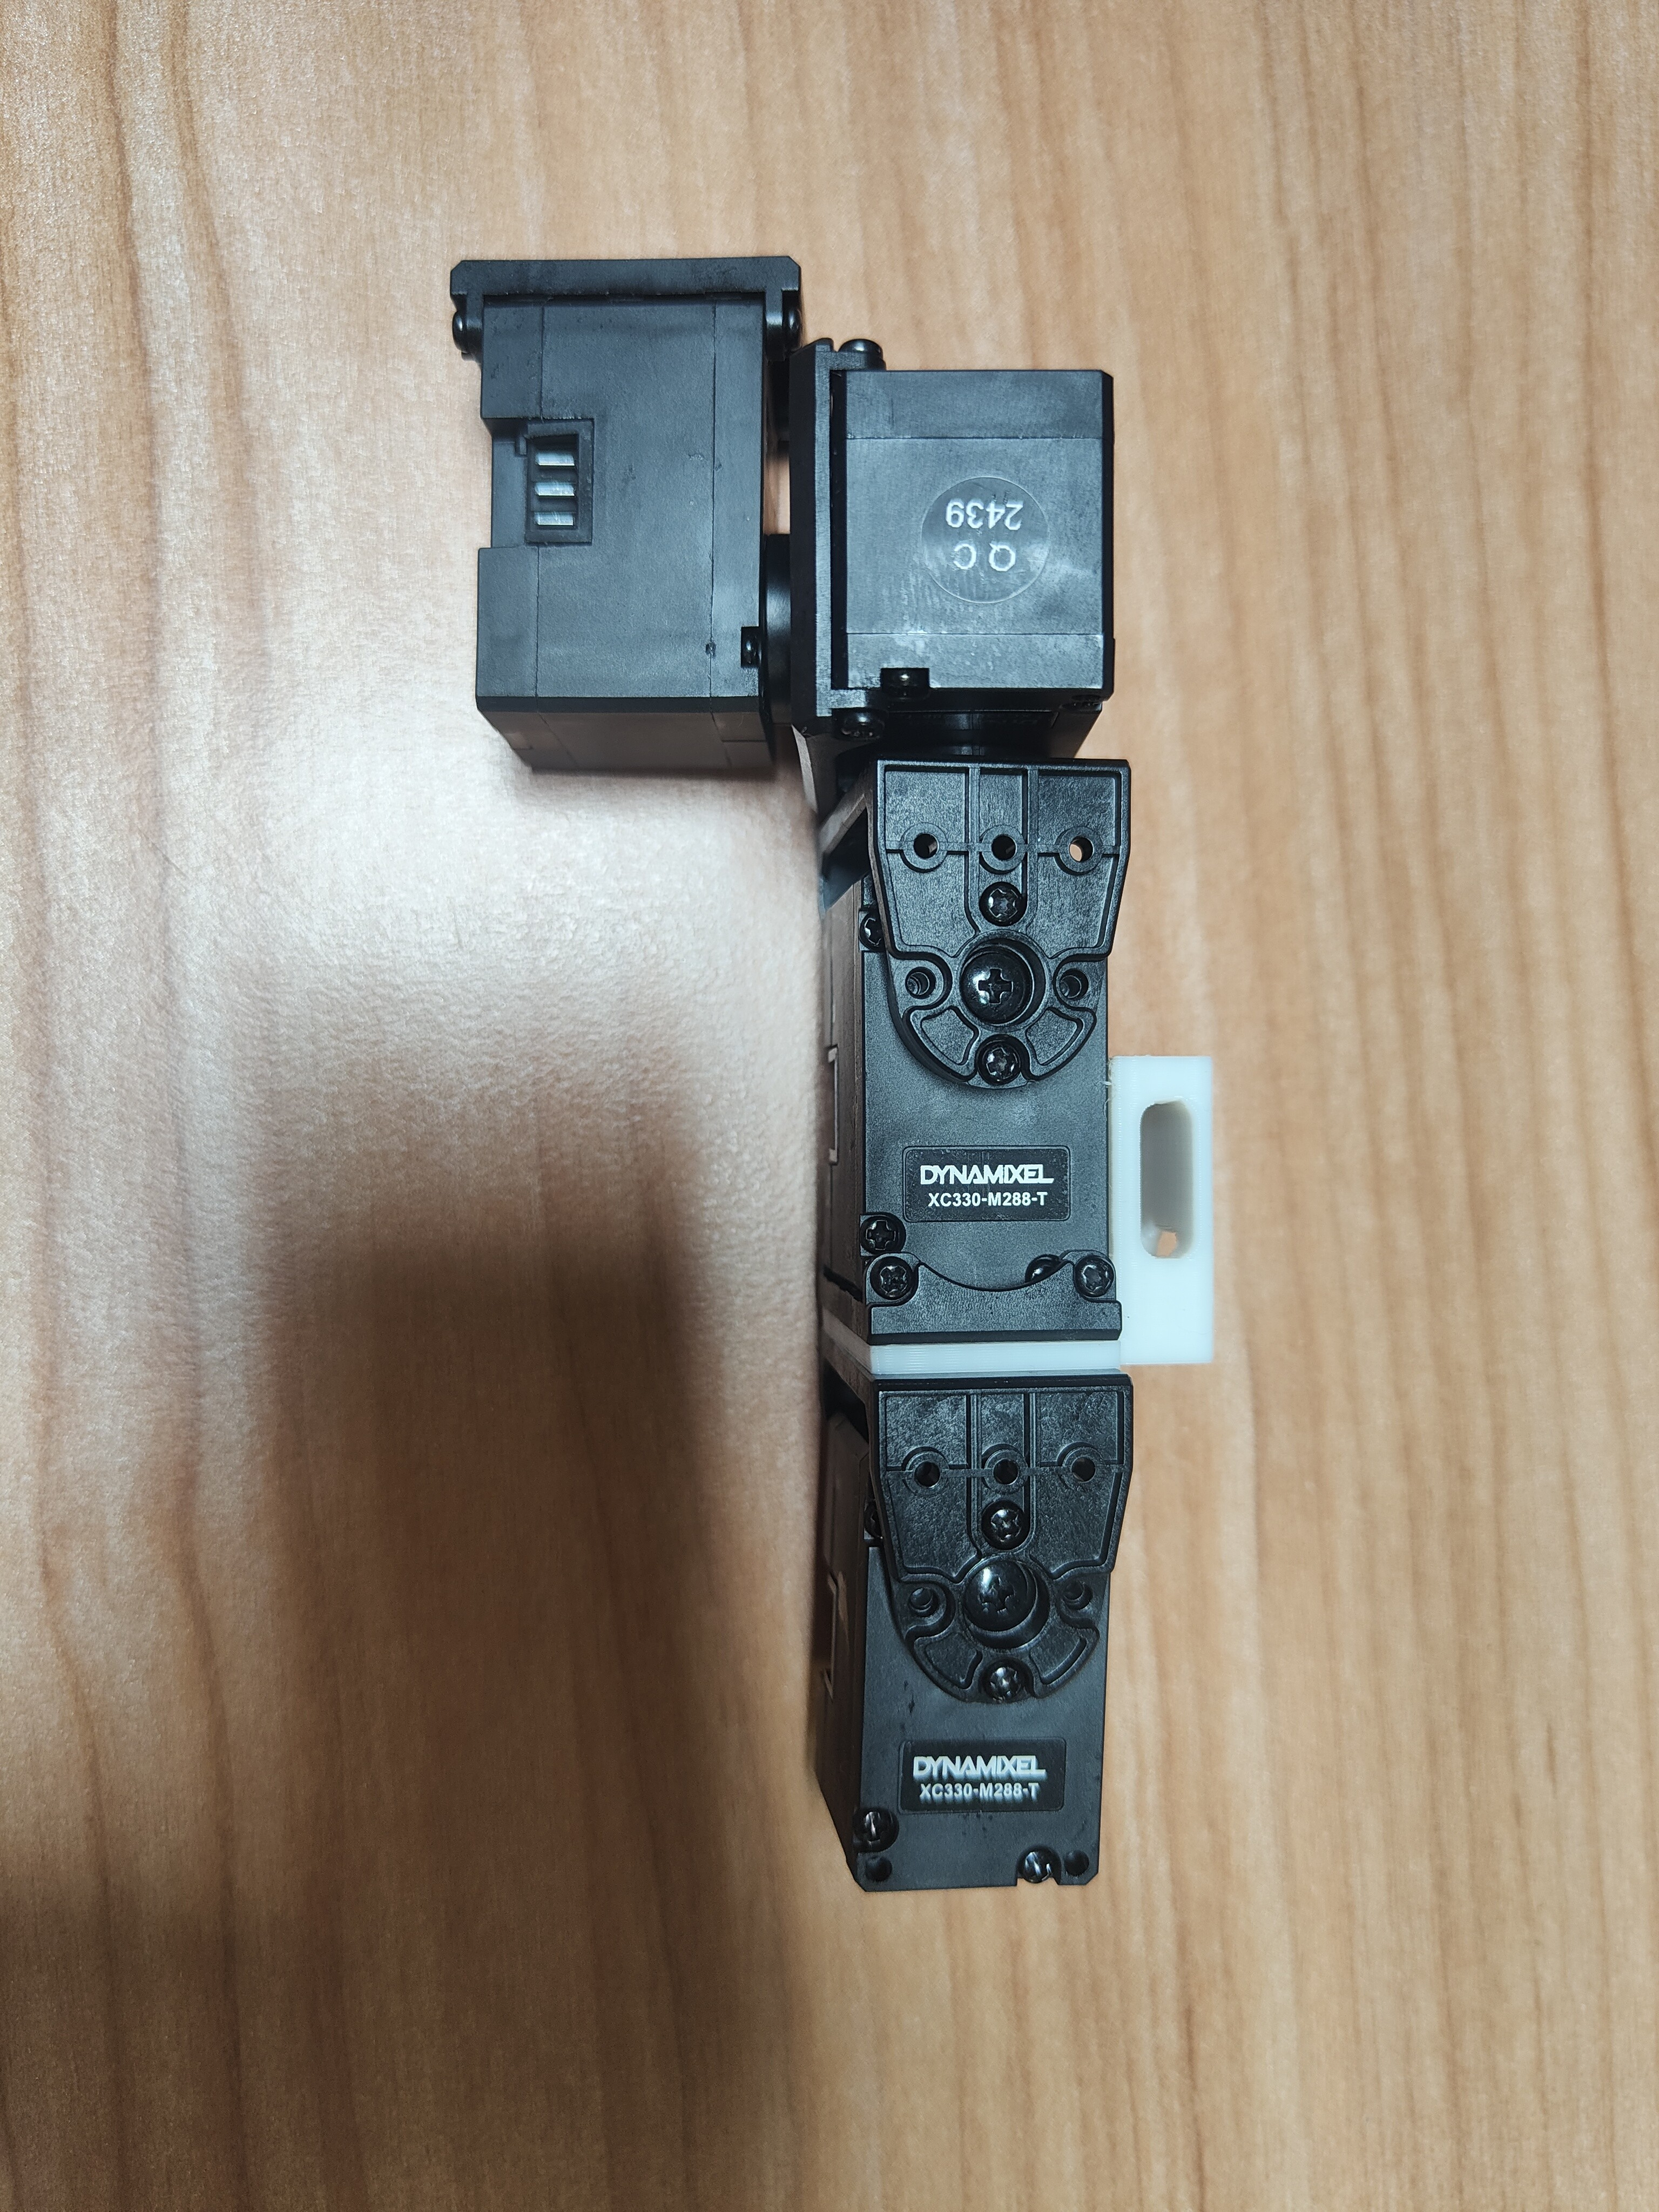
\includegraphics[width=0.25\textwidth]{figs/appendix/polegar/7.jpg} &
  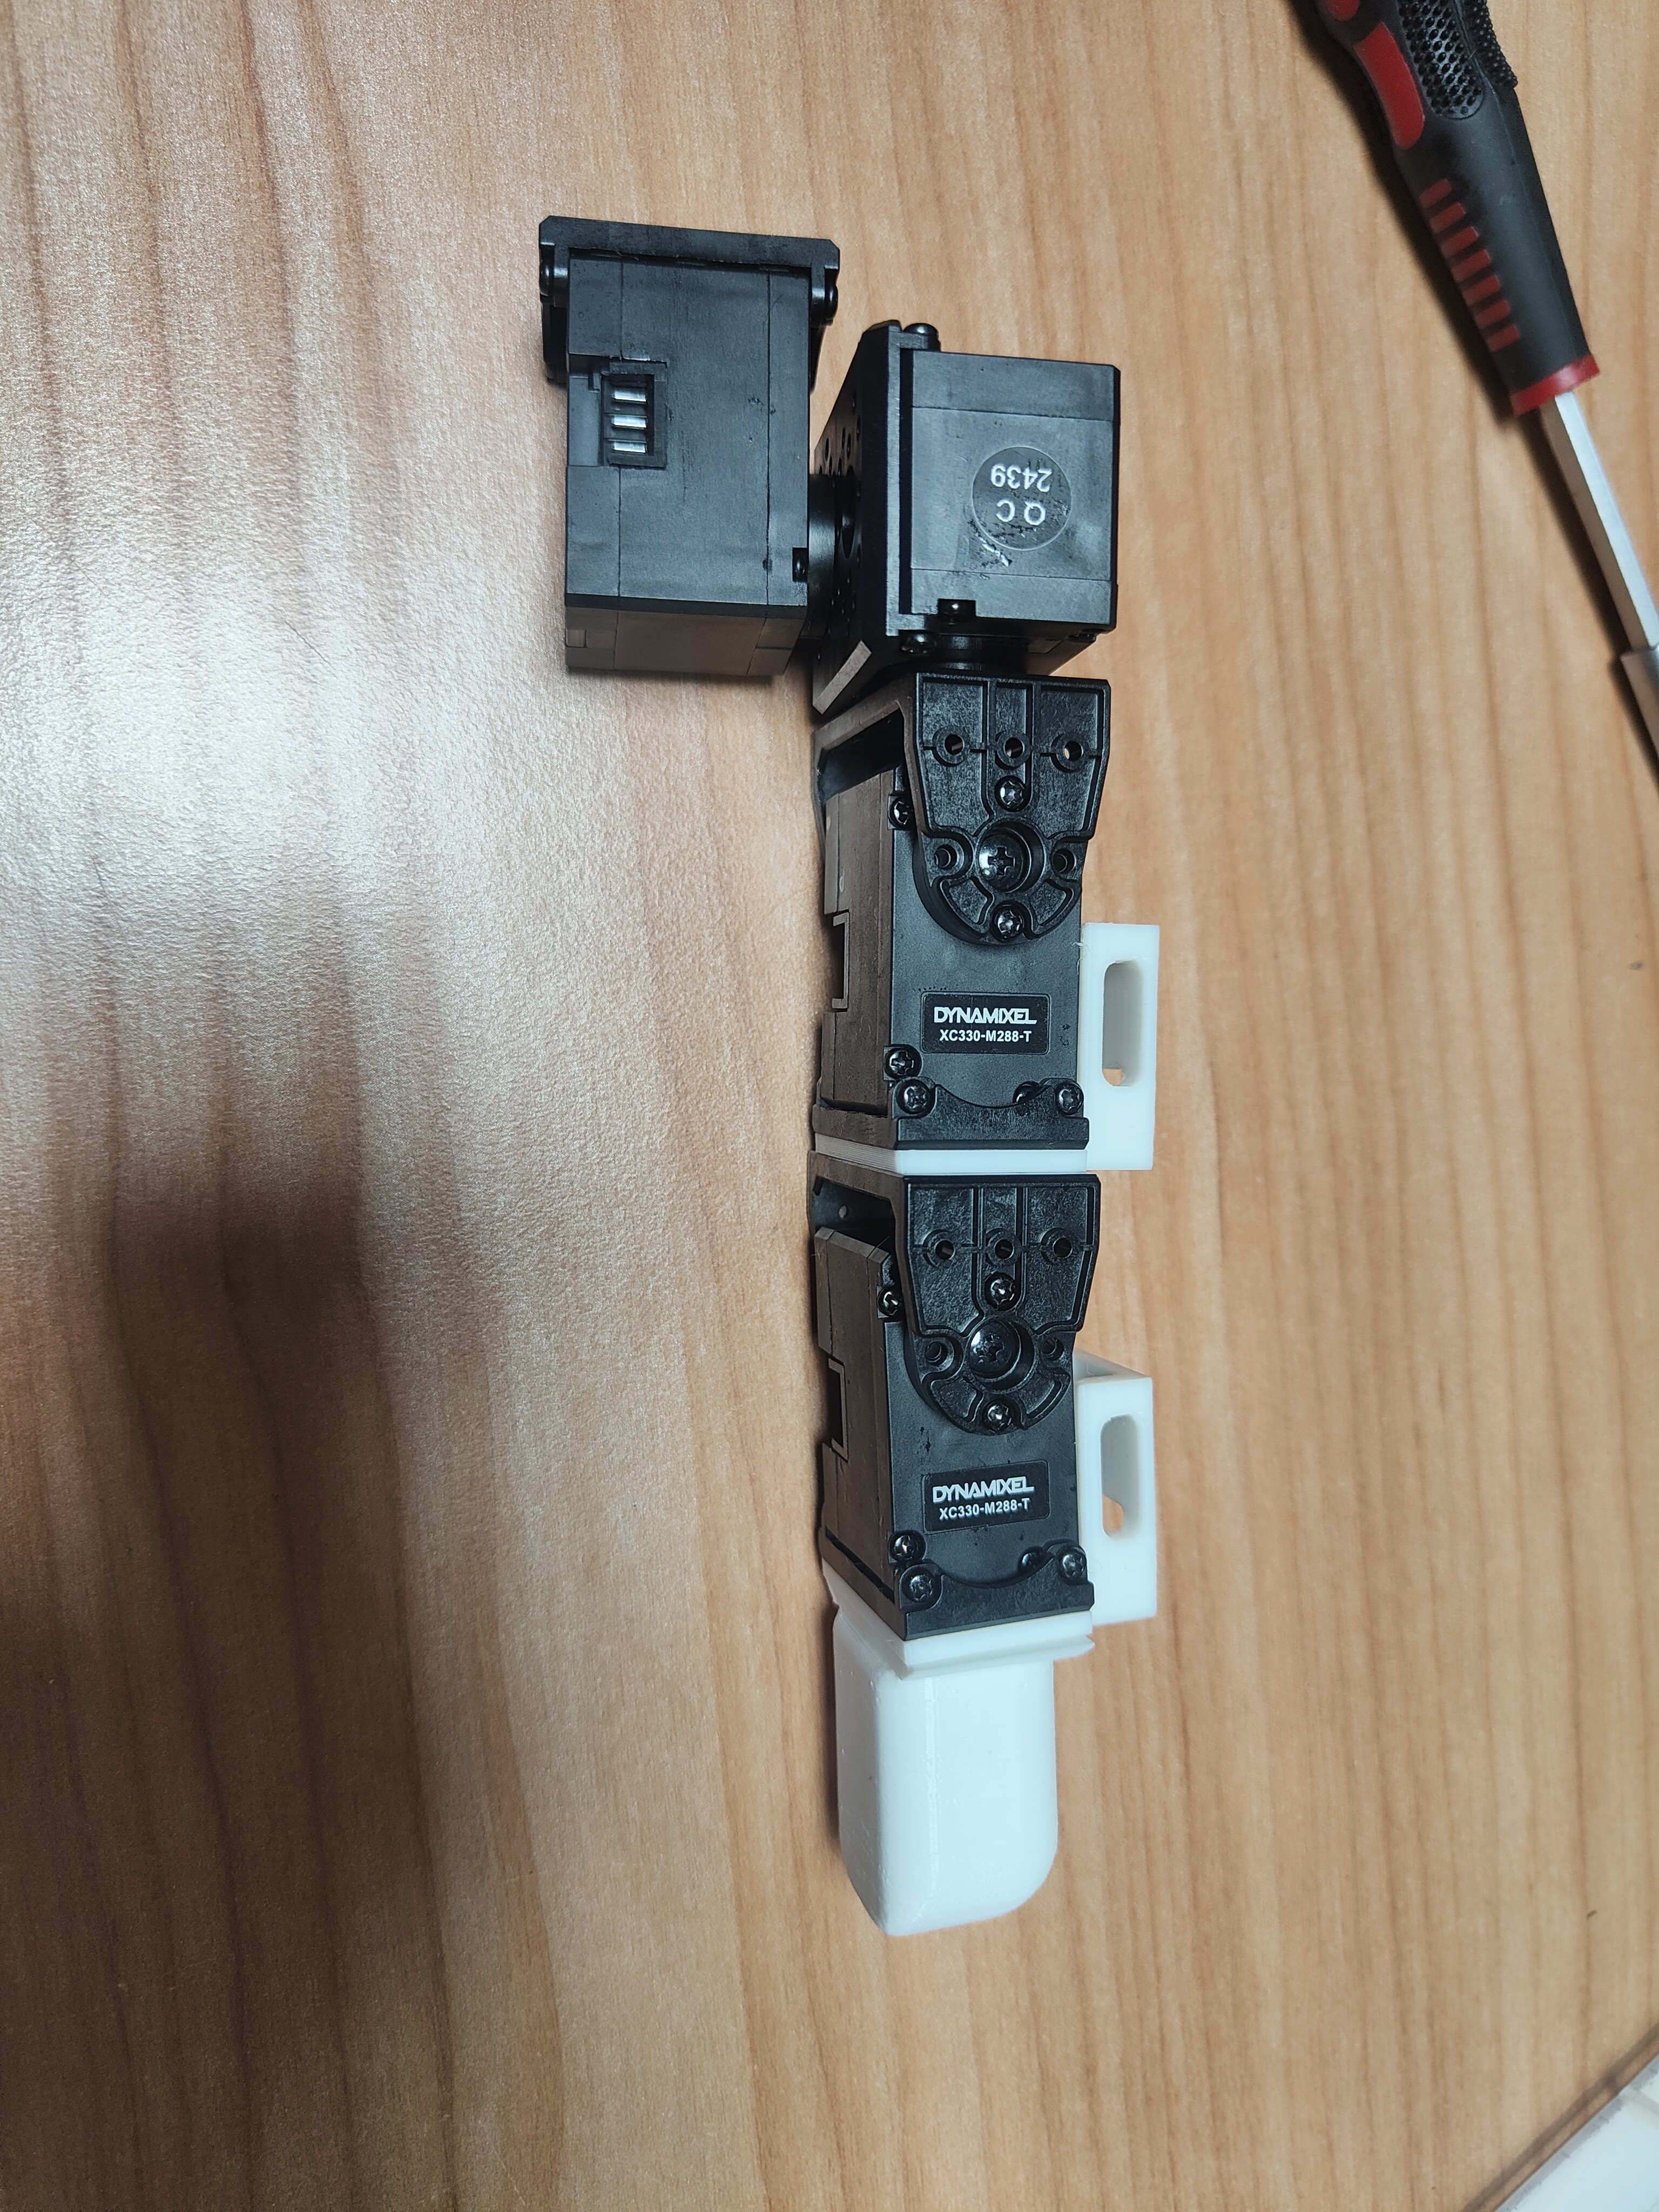
\includegraphics[width=0.25\textwidth]{figs/appendix/polegar/8.jpg} &
  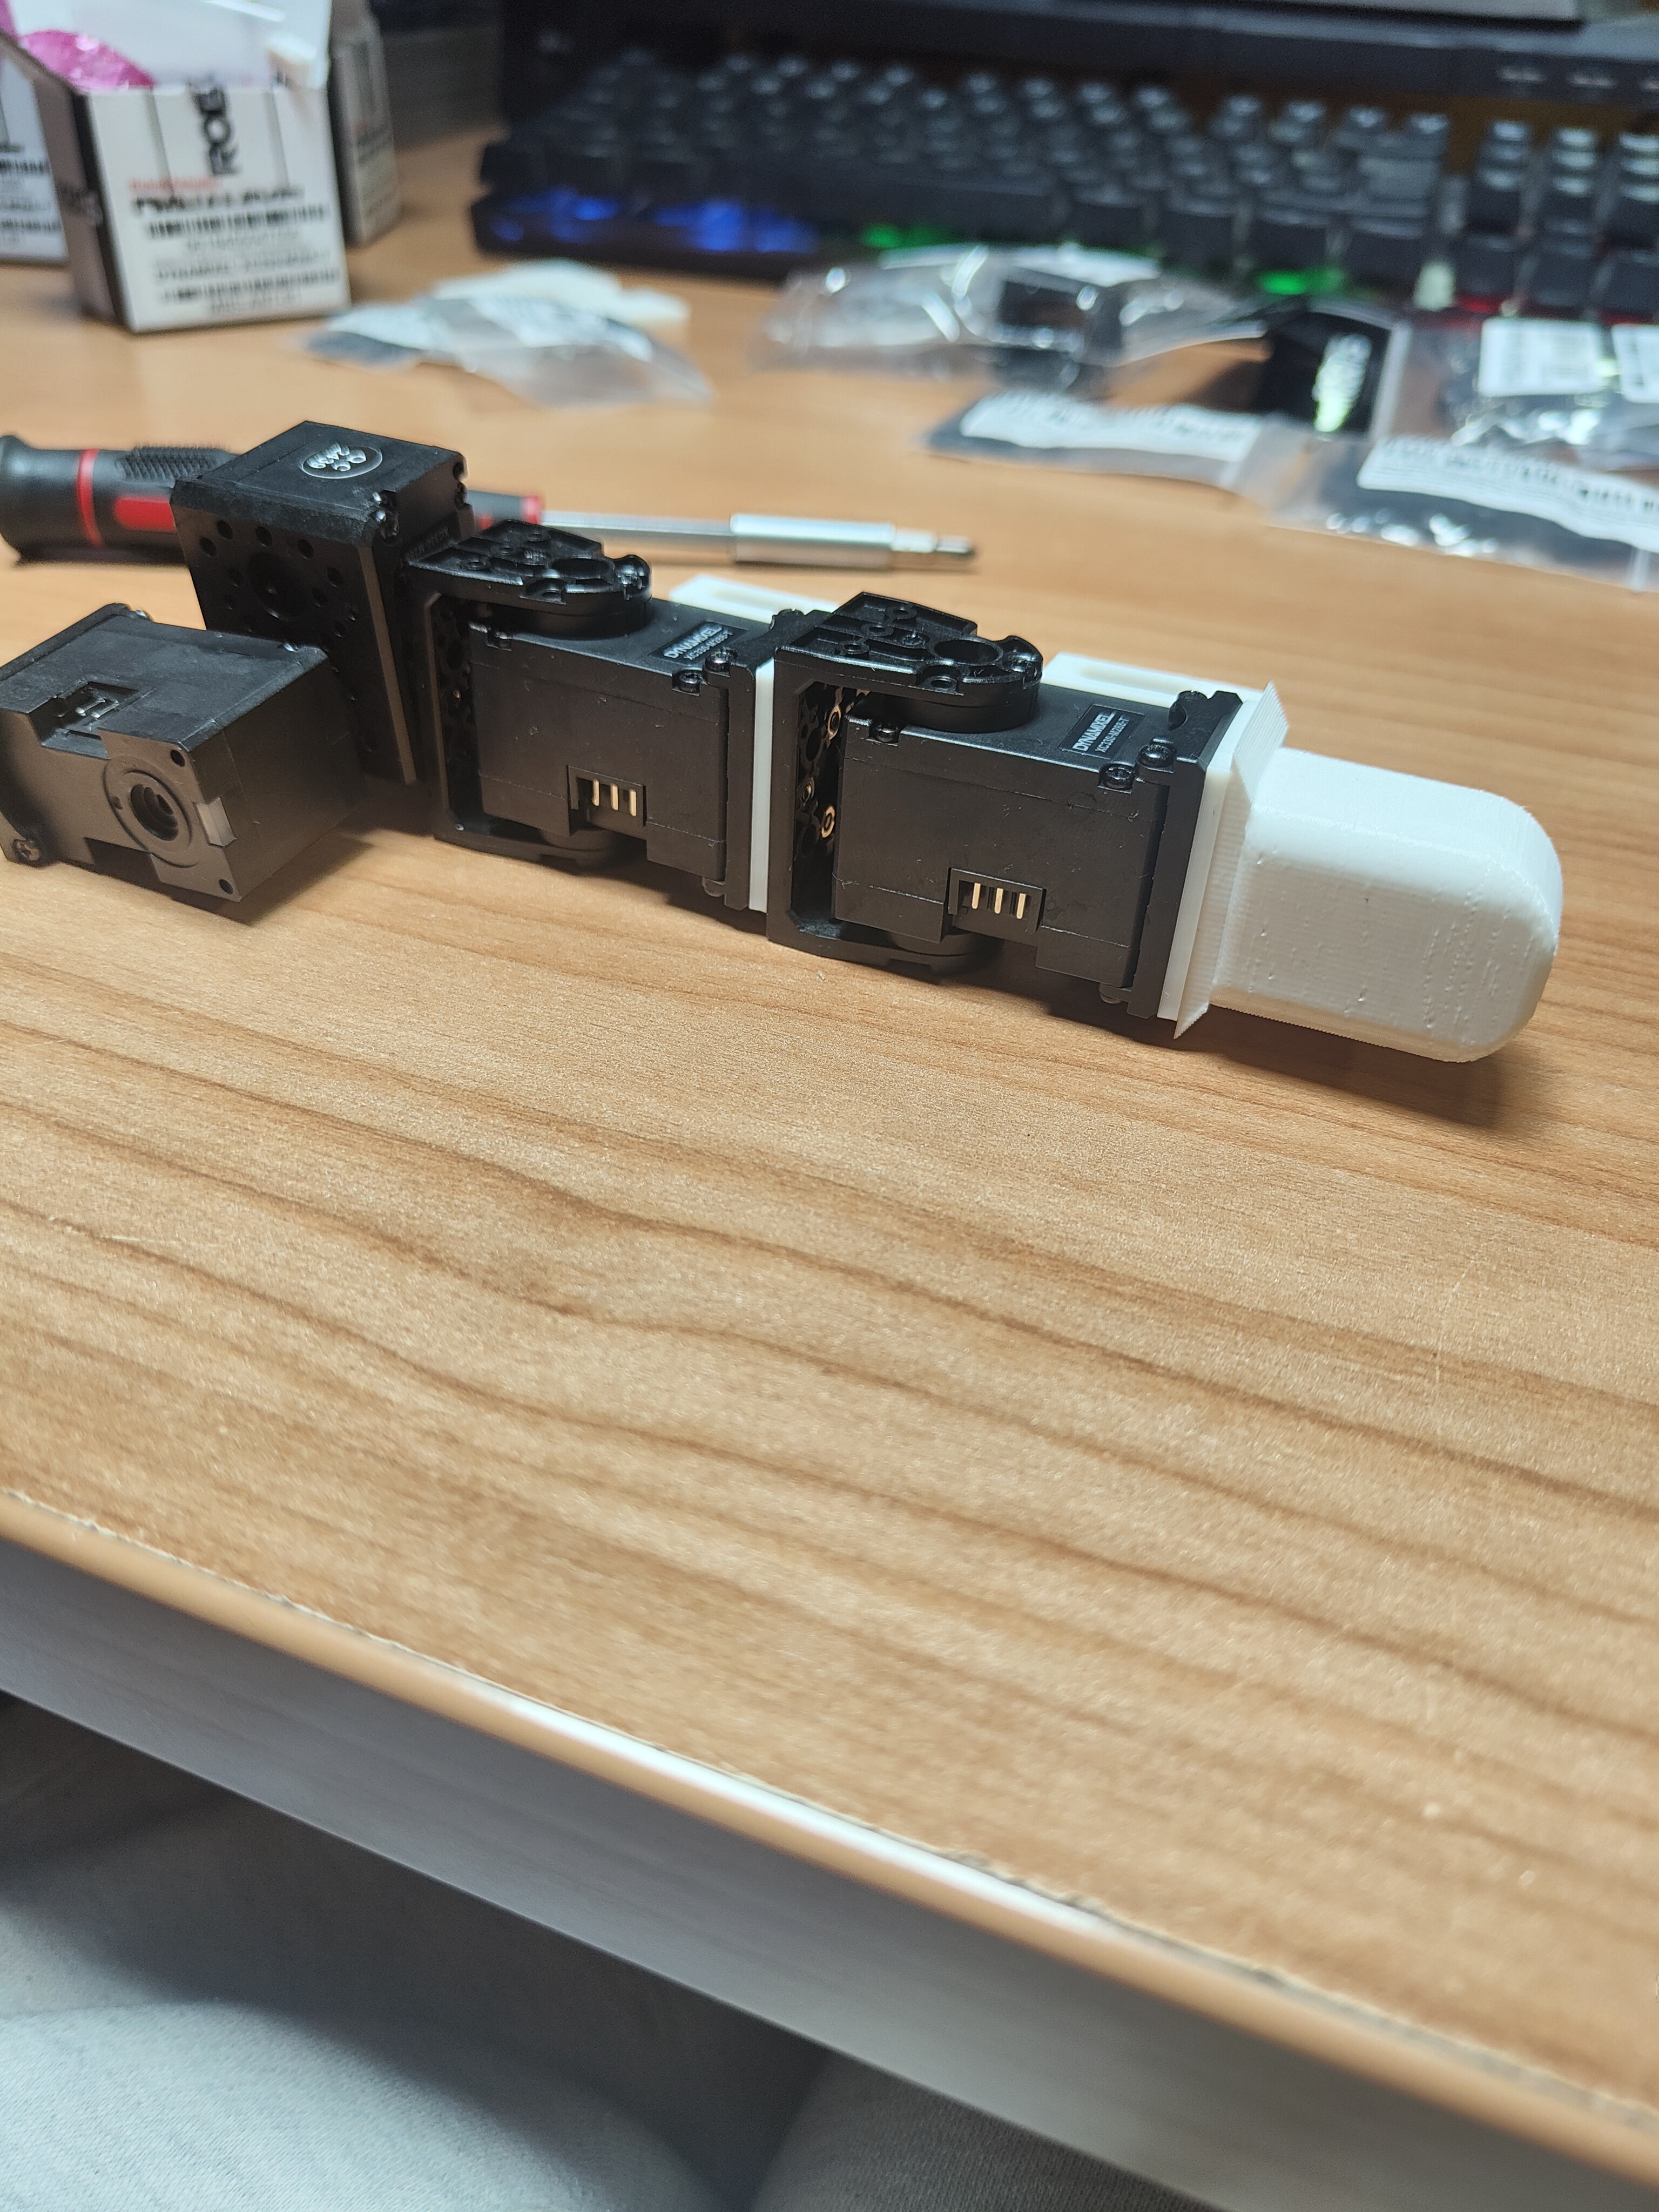
\includegraphics[width=0.25\textwidth]{figs/appendix/polegar/9.jpg} \\
\end{tabular}
\caption{Fotografias sequenciais da montagem do polegar}
\end{figure}
\label{appendix:montagem_polegar}

\subsection{Montagem dos restantes dedos}

\begin{figure}[H]
\centering
\begin{tabular}{ccc}
  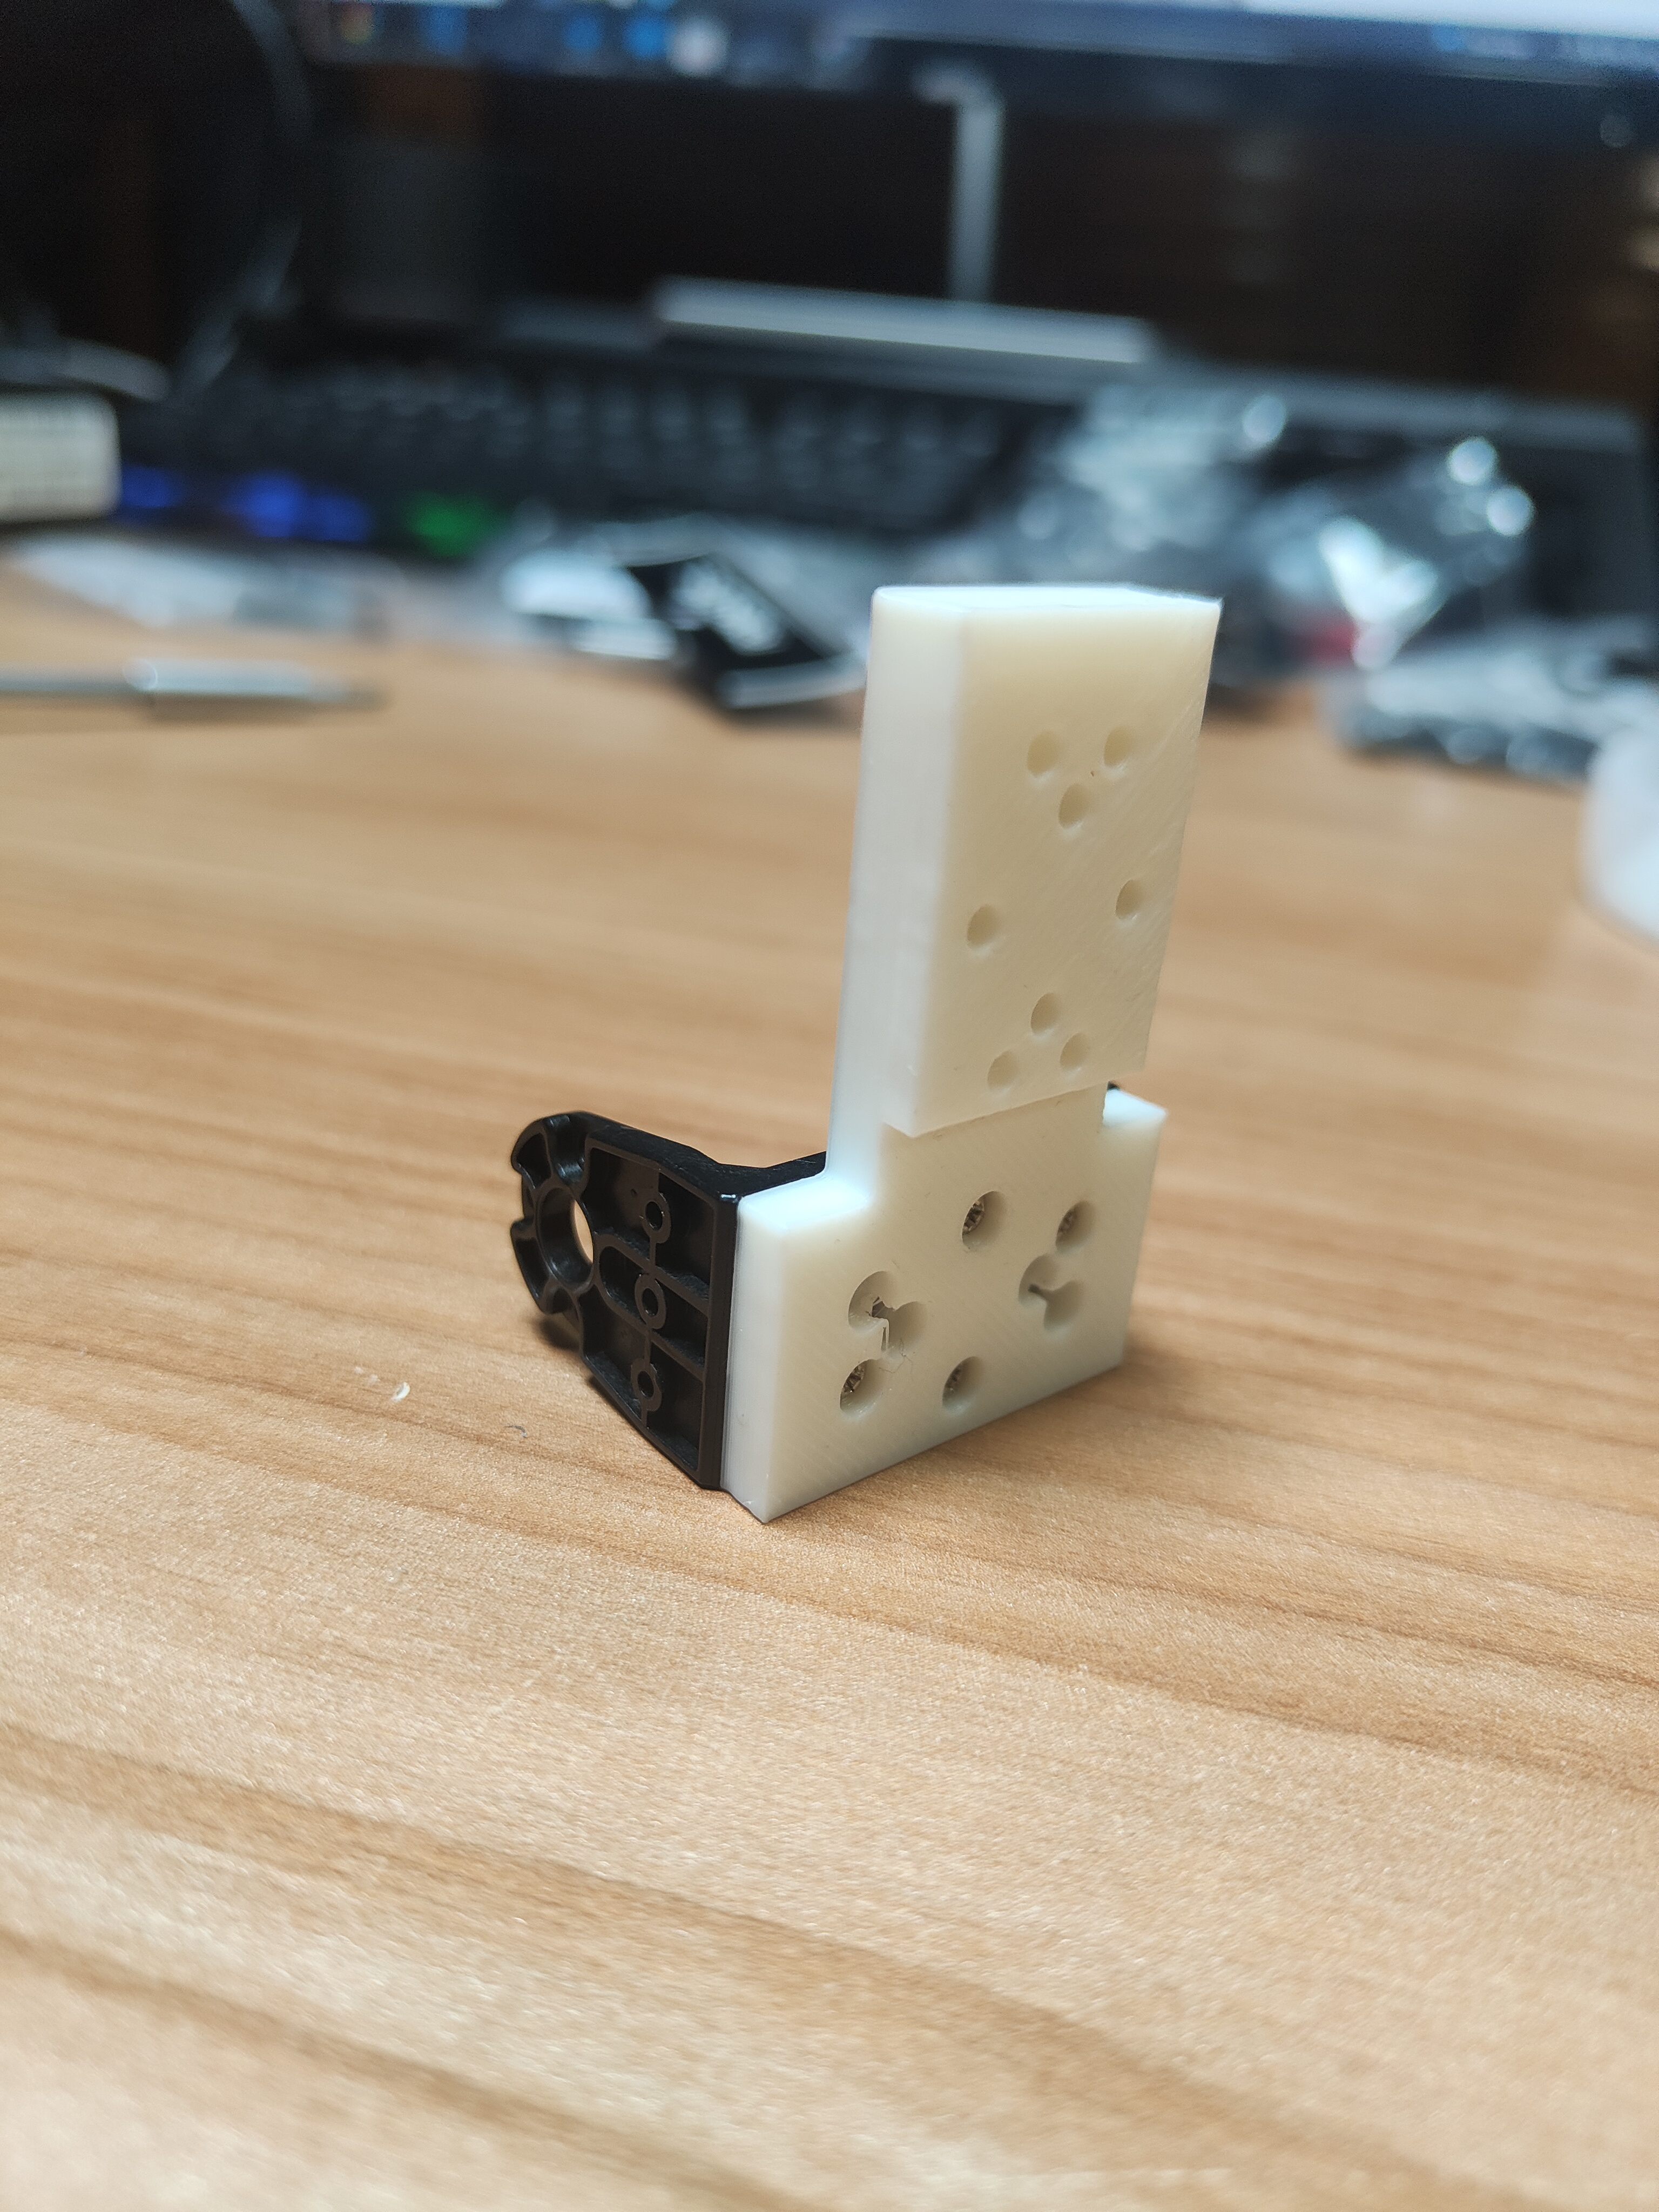
\includegraphics[width=0.25\textwidth]{figs/appendix/dedo/1.jpg} &
  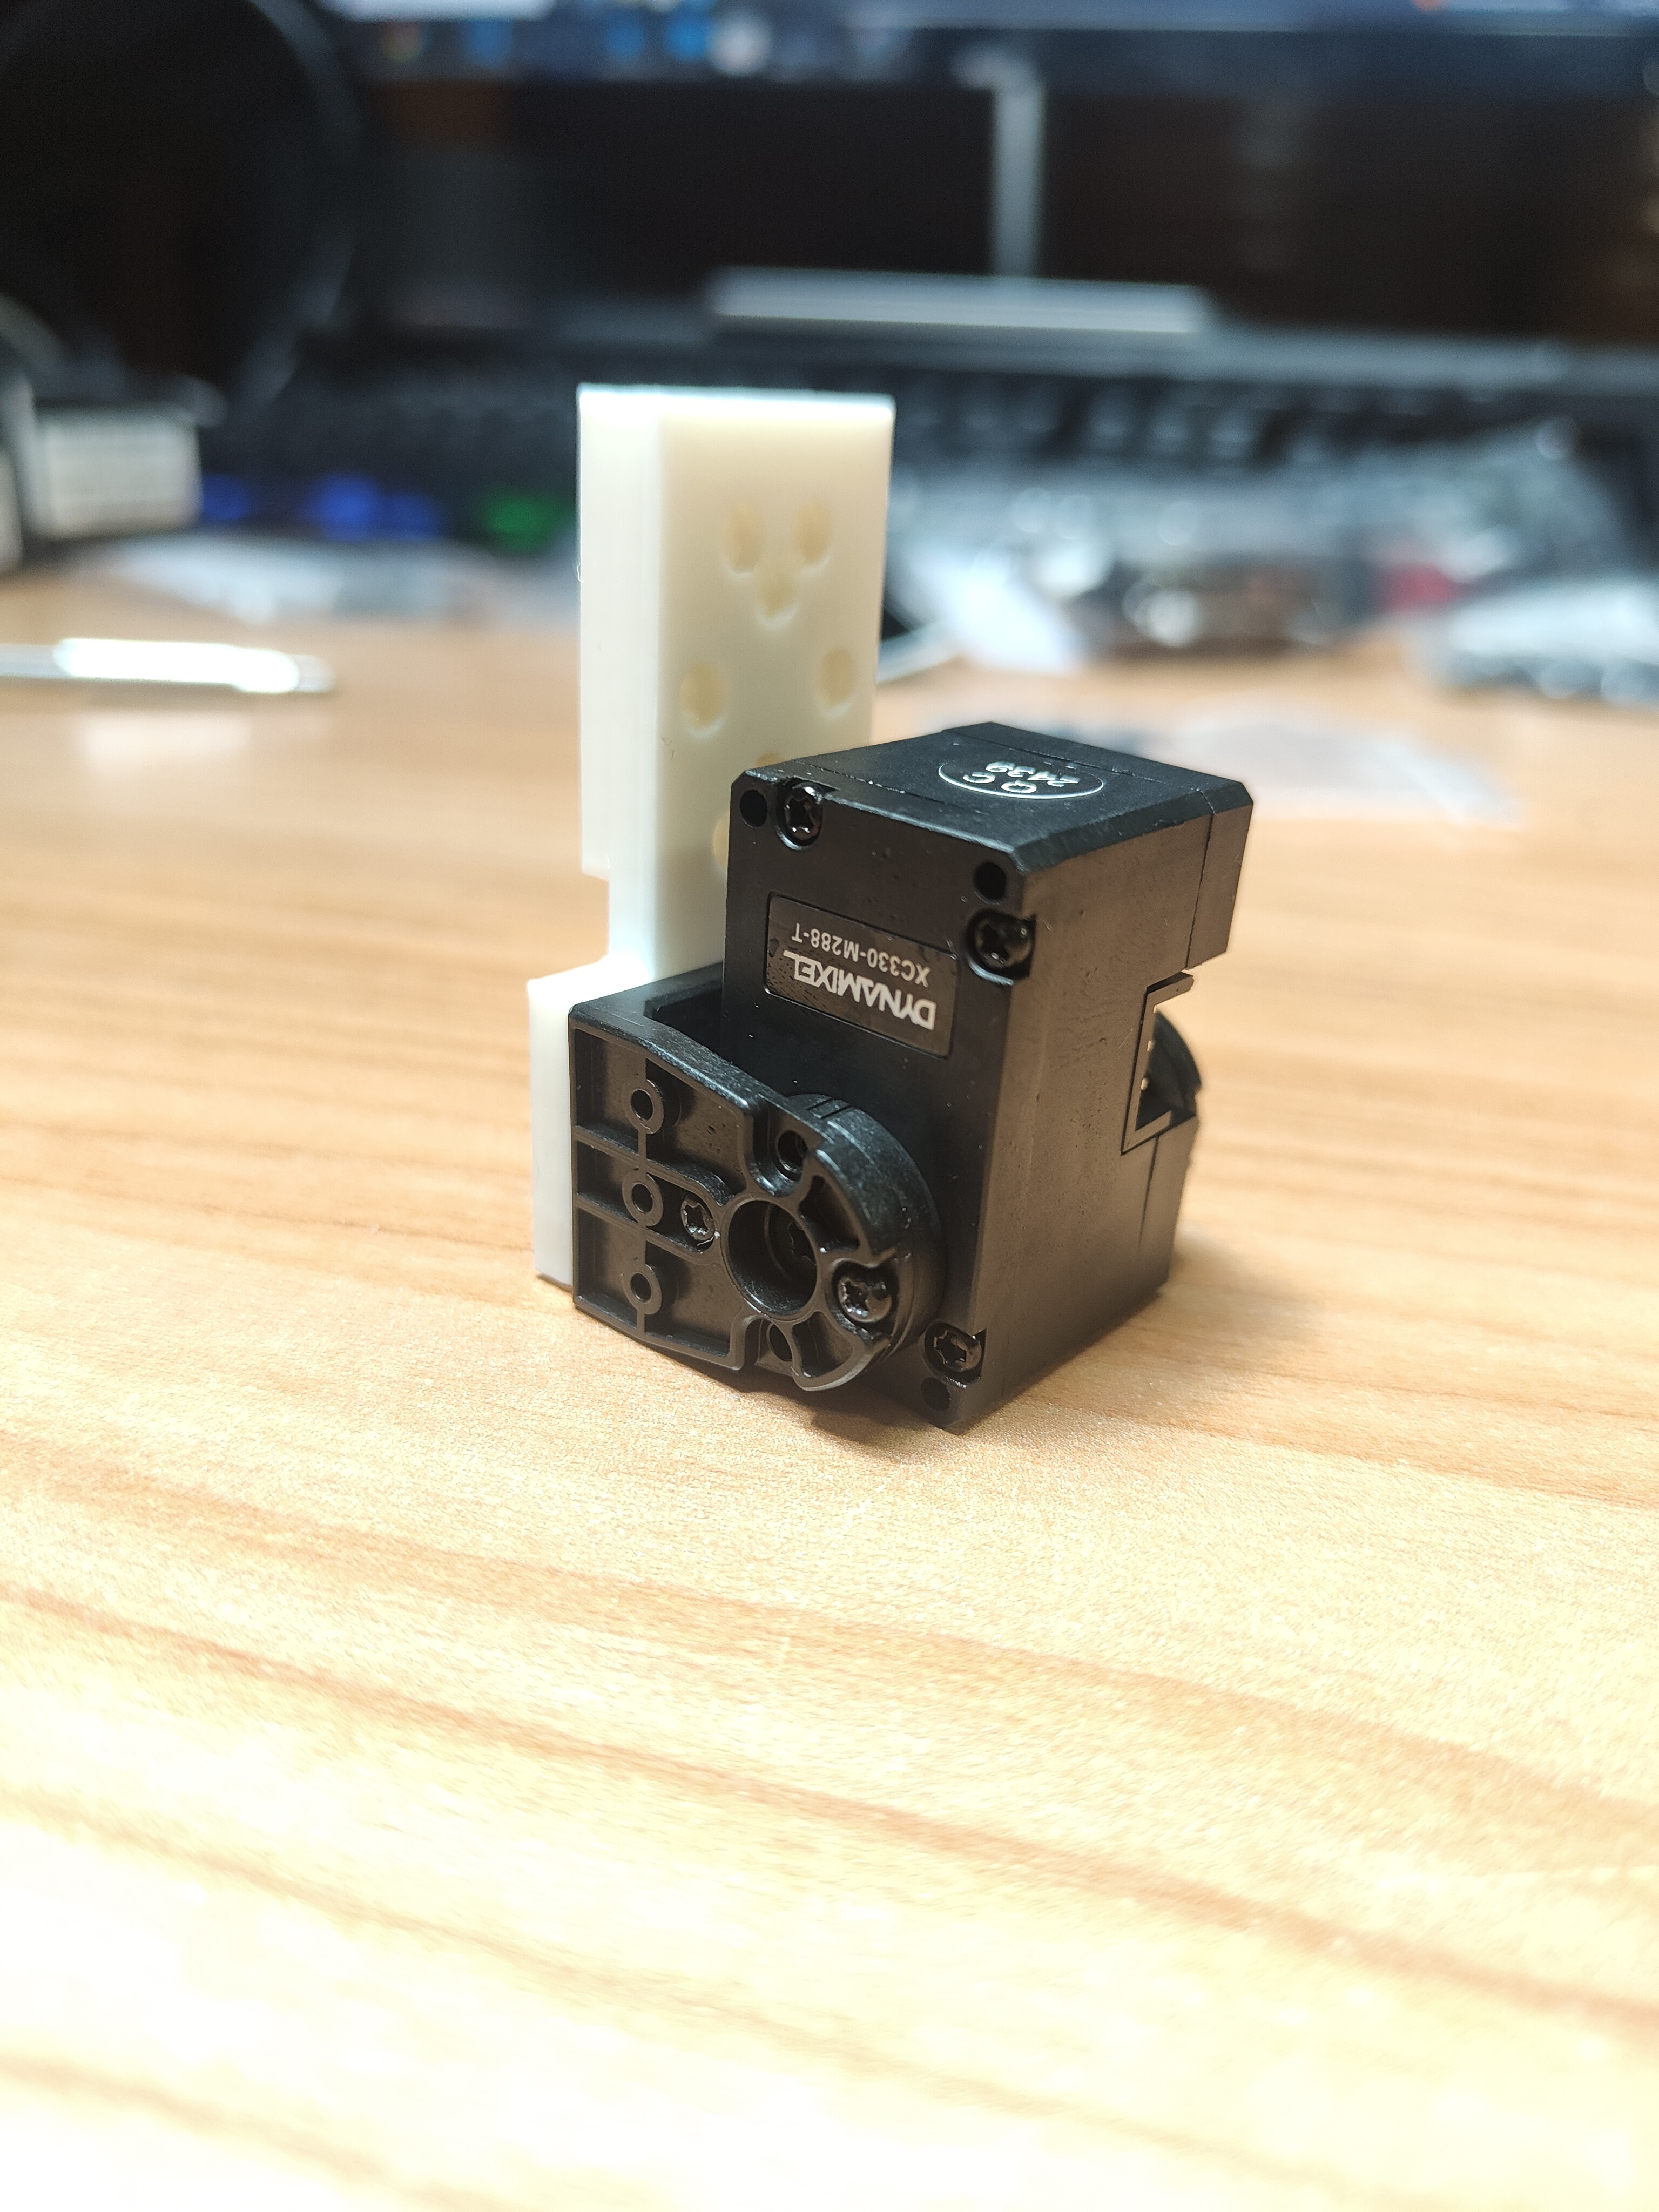
\includegraphics[width=0.25\textwidth]{figs/appendix/dedo/2.jpg} &
  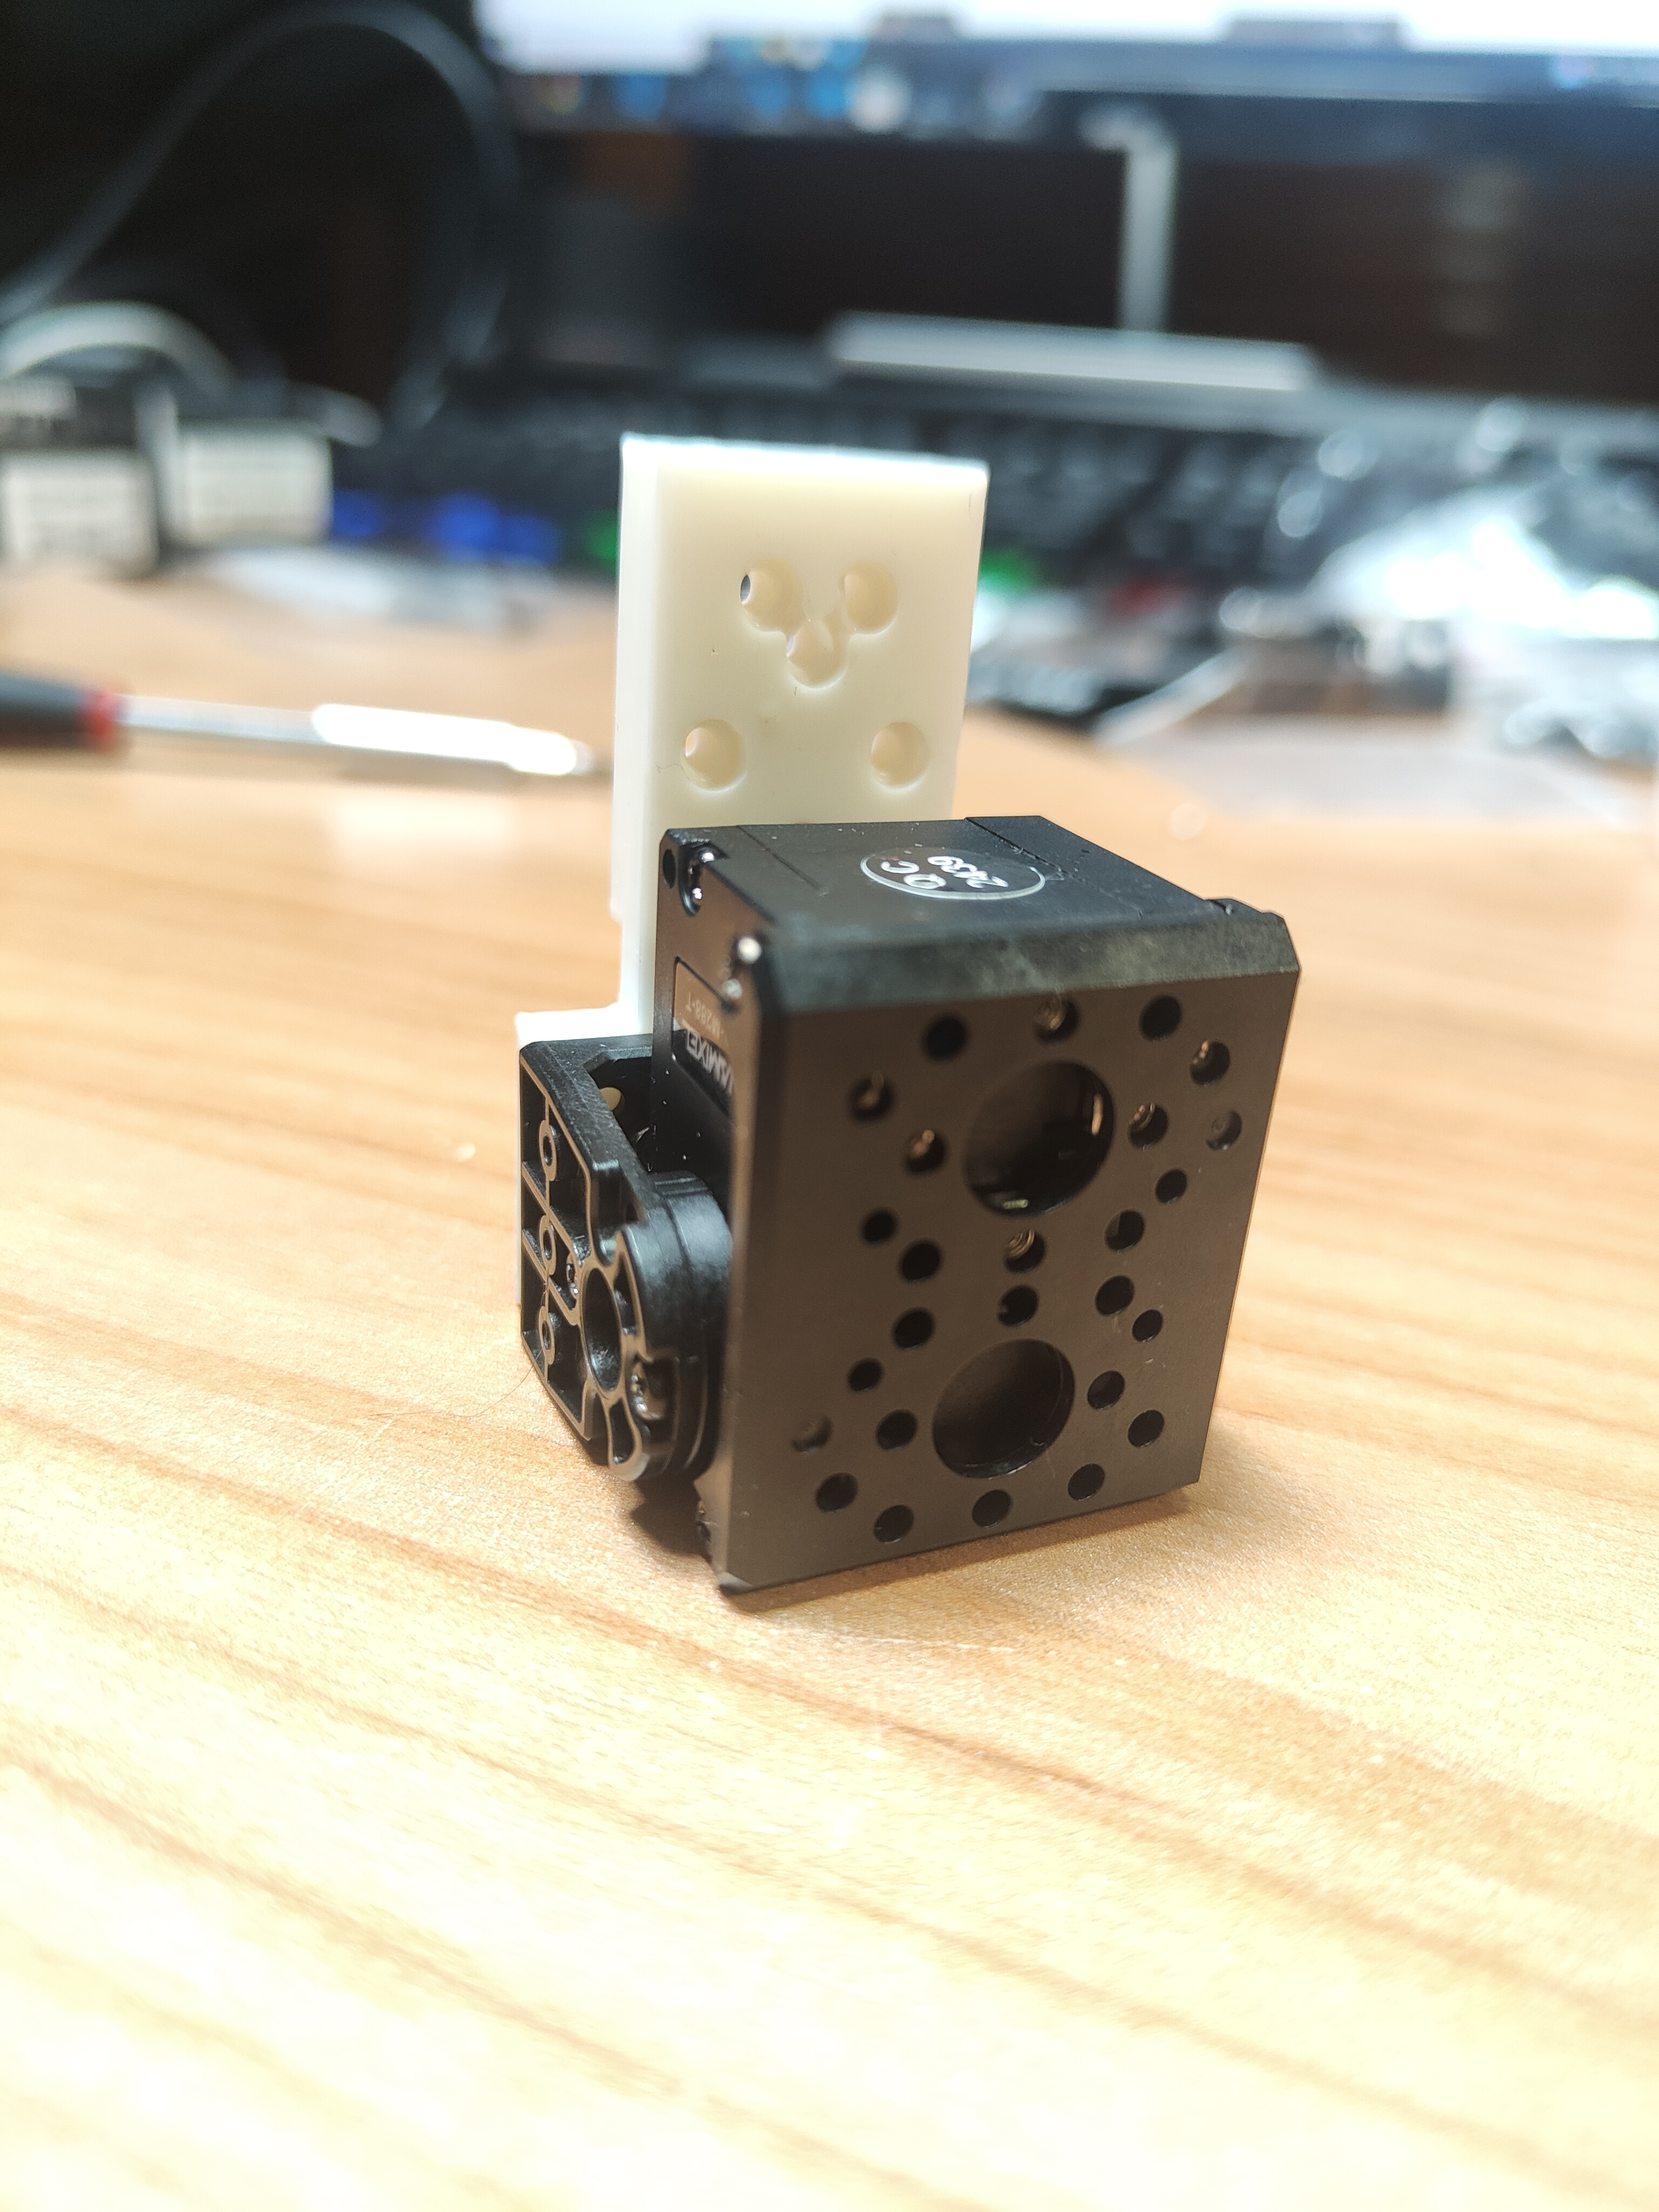
\includegraphics[width=0.25\textwidth]{figs/appendix/dedo/3.jpg} \\
  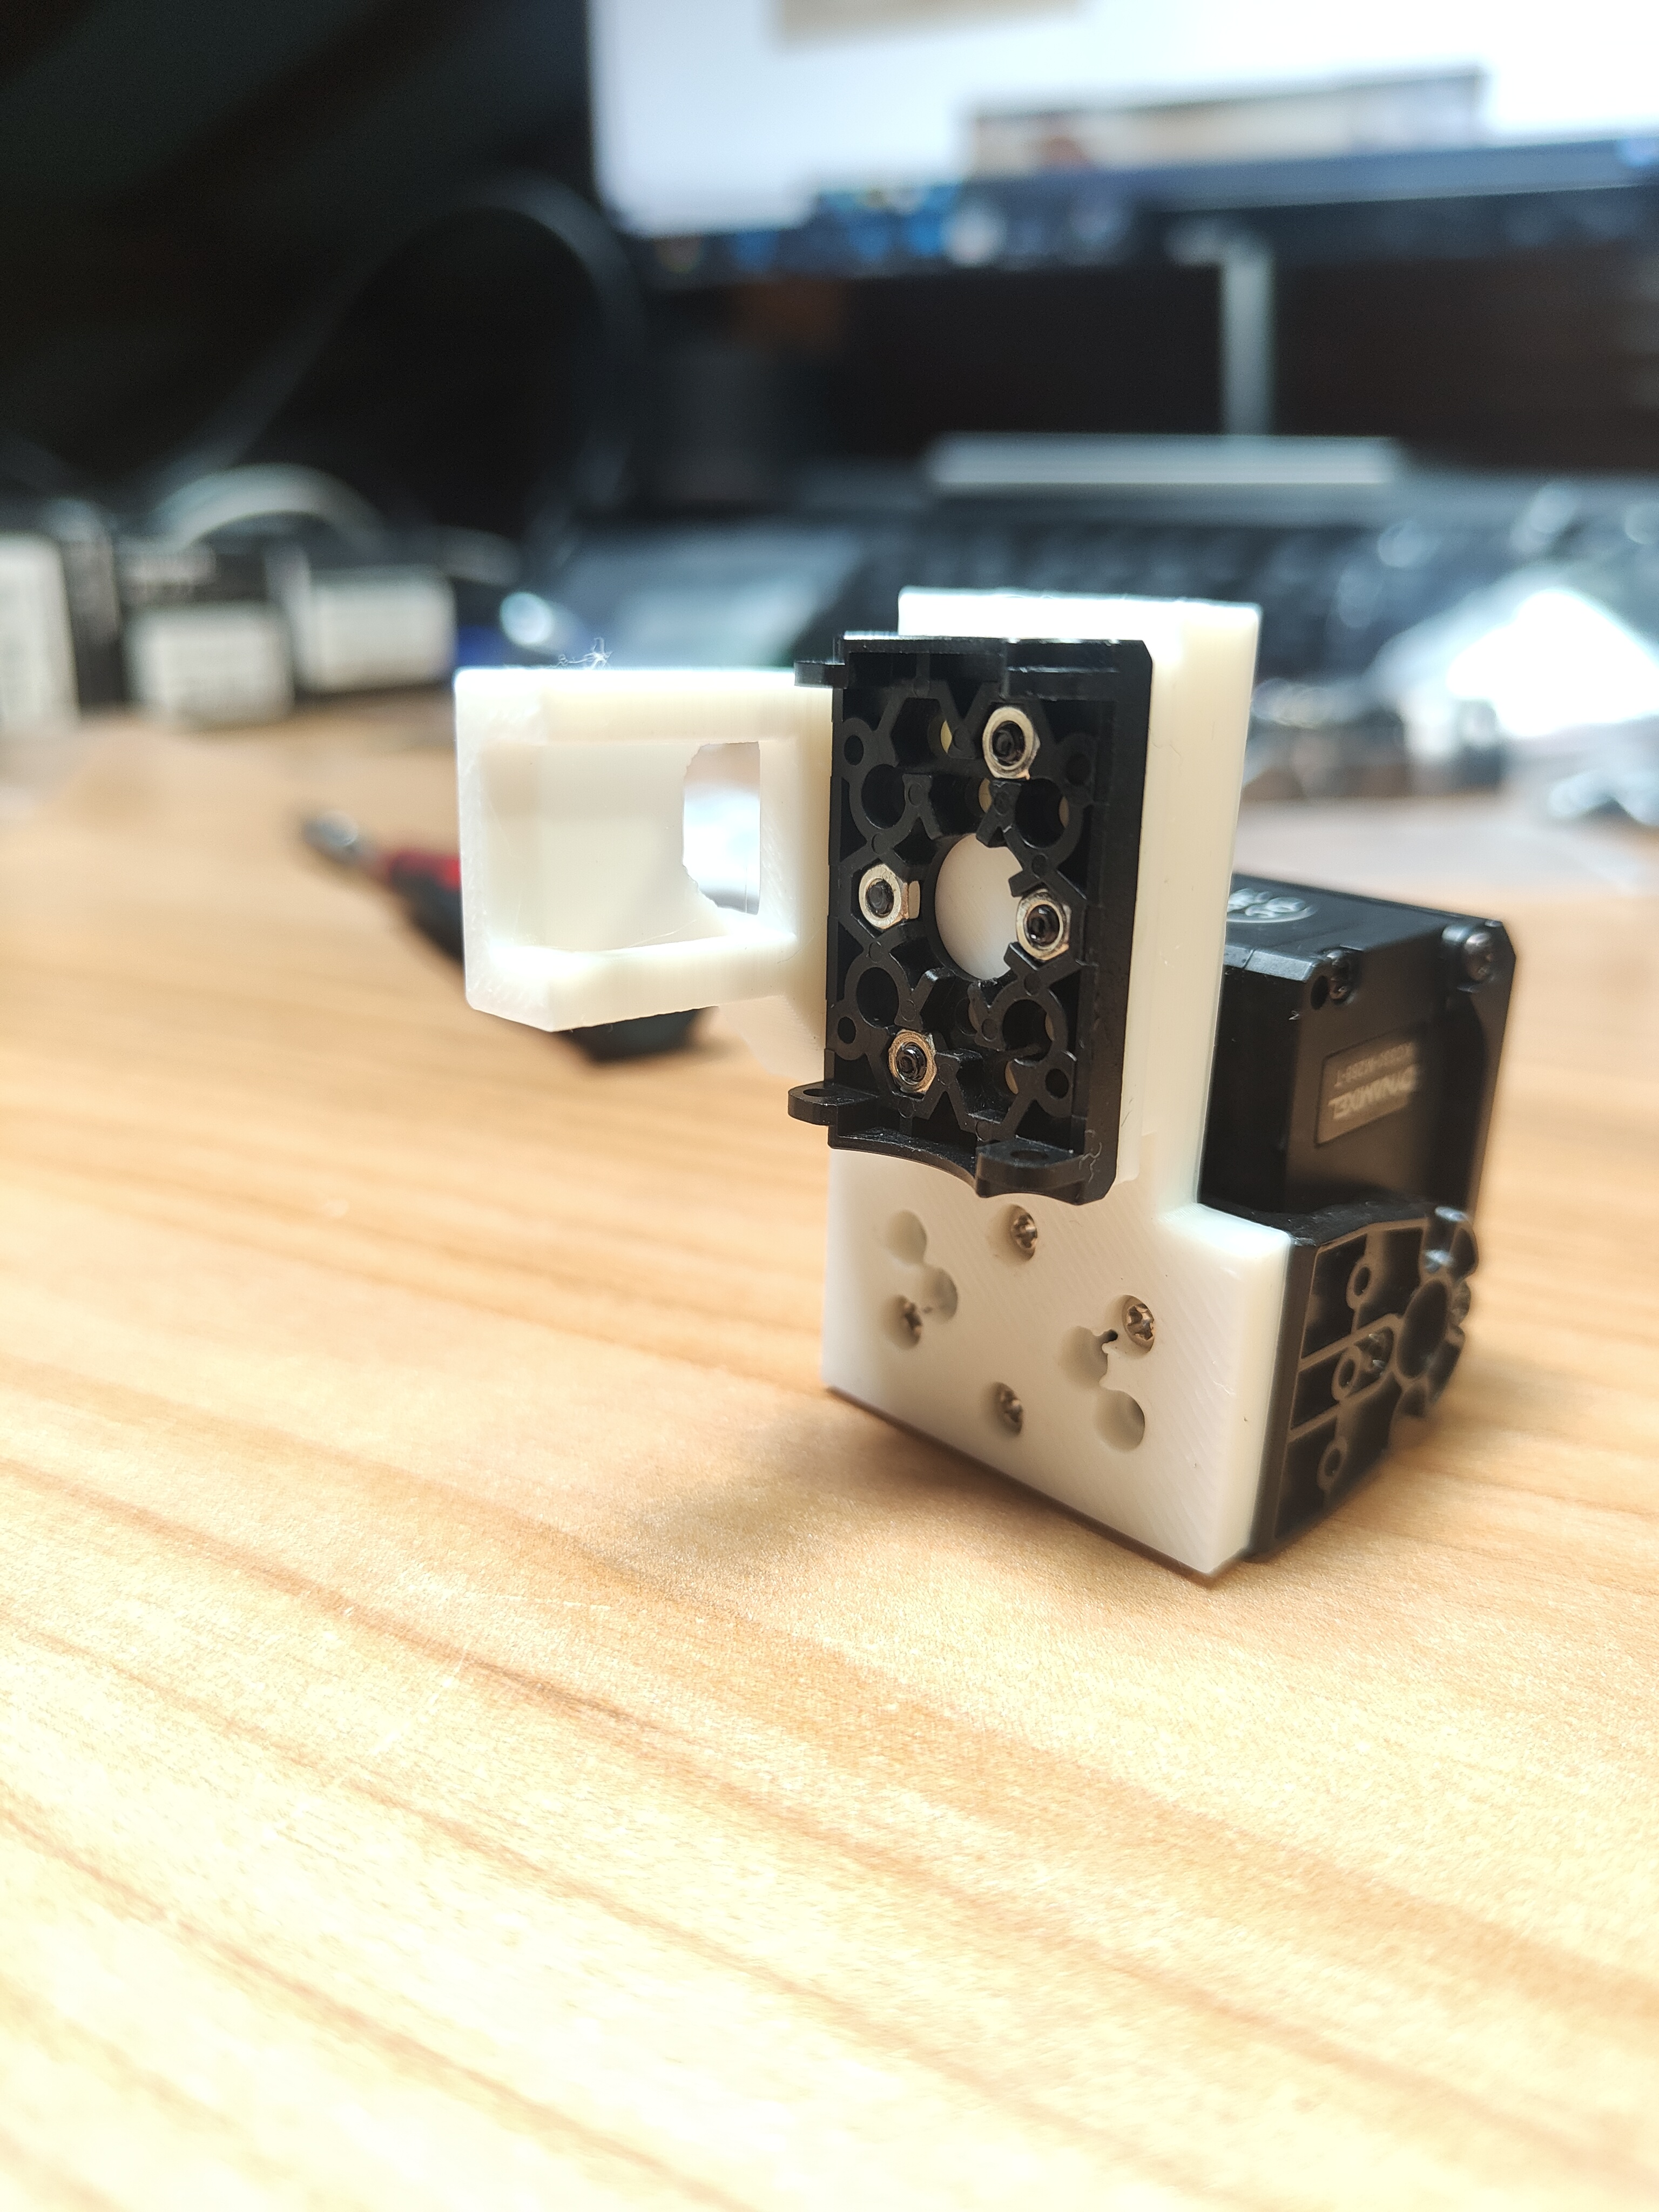
\includegraphics[width=0.25\textwidth]{figs/appendix/dedo/4.jpg} &
  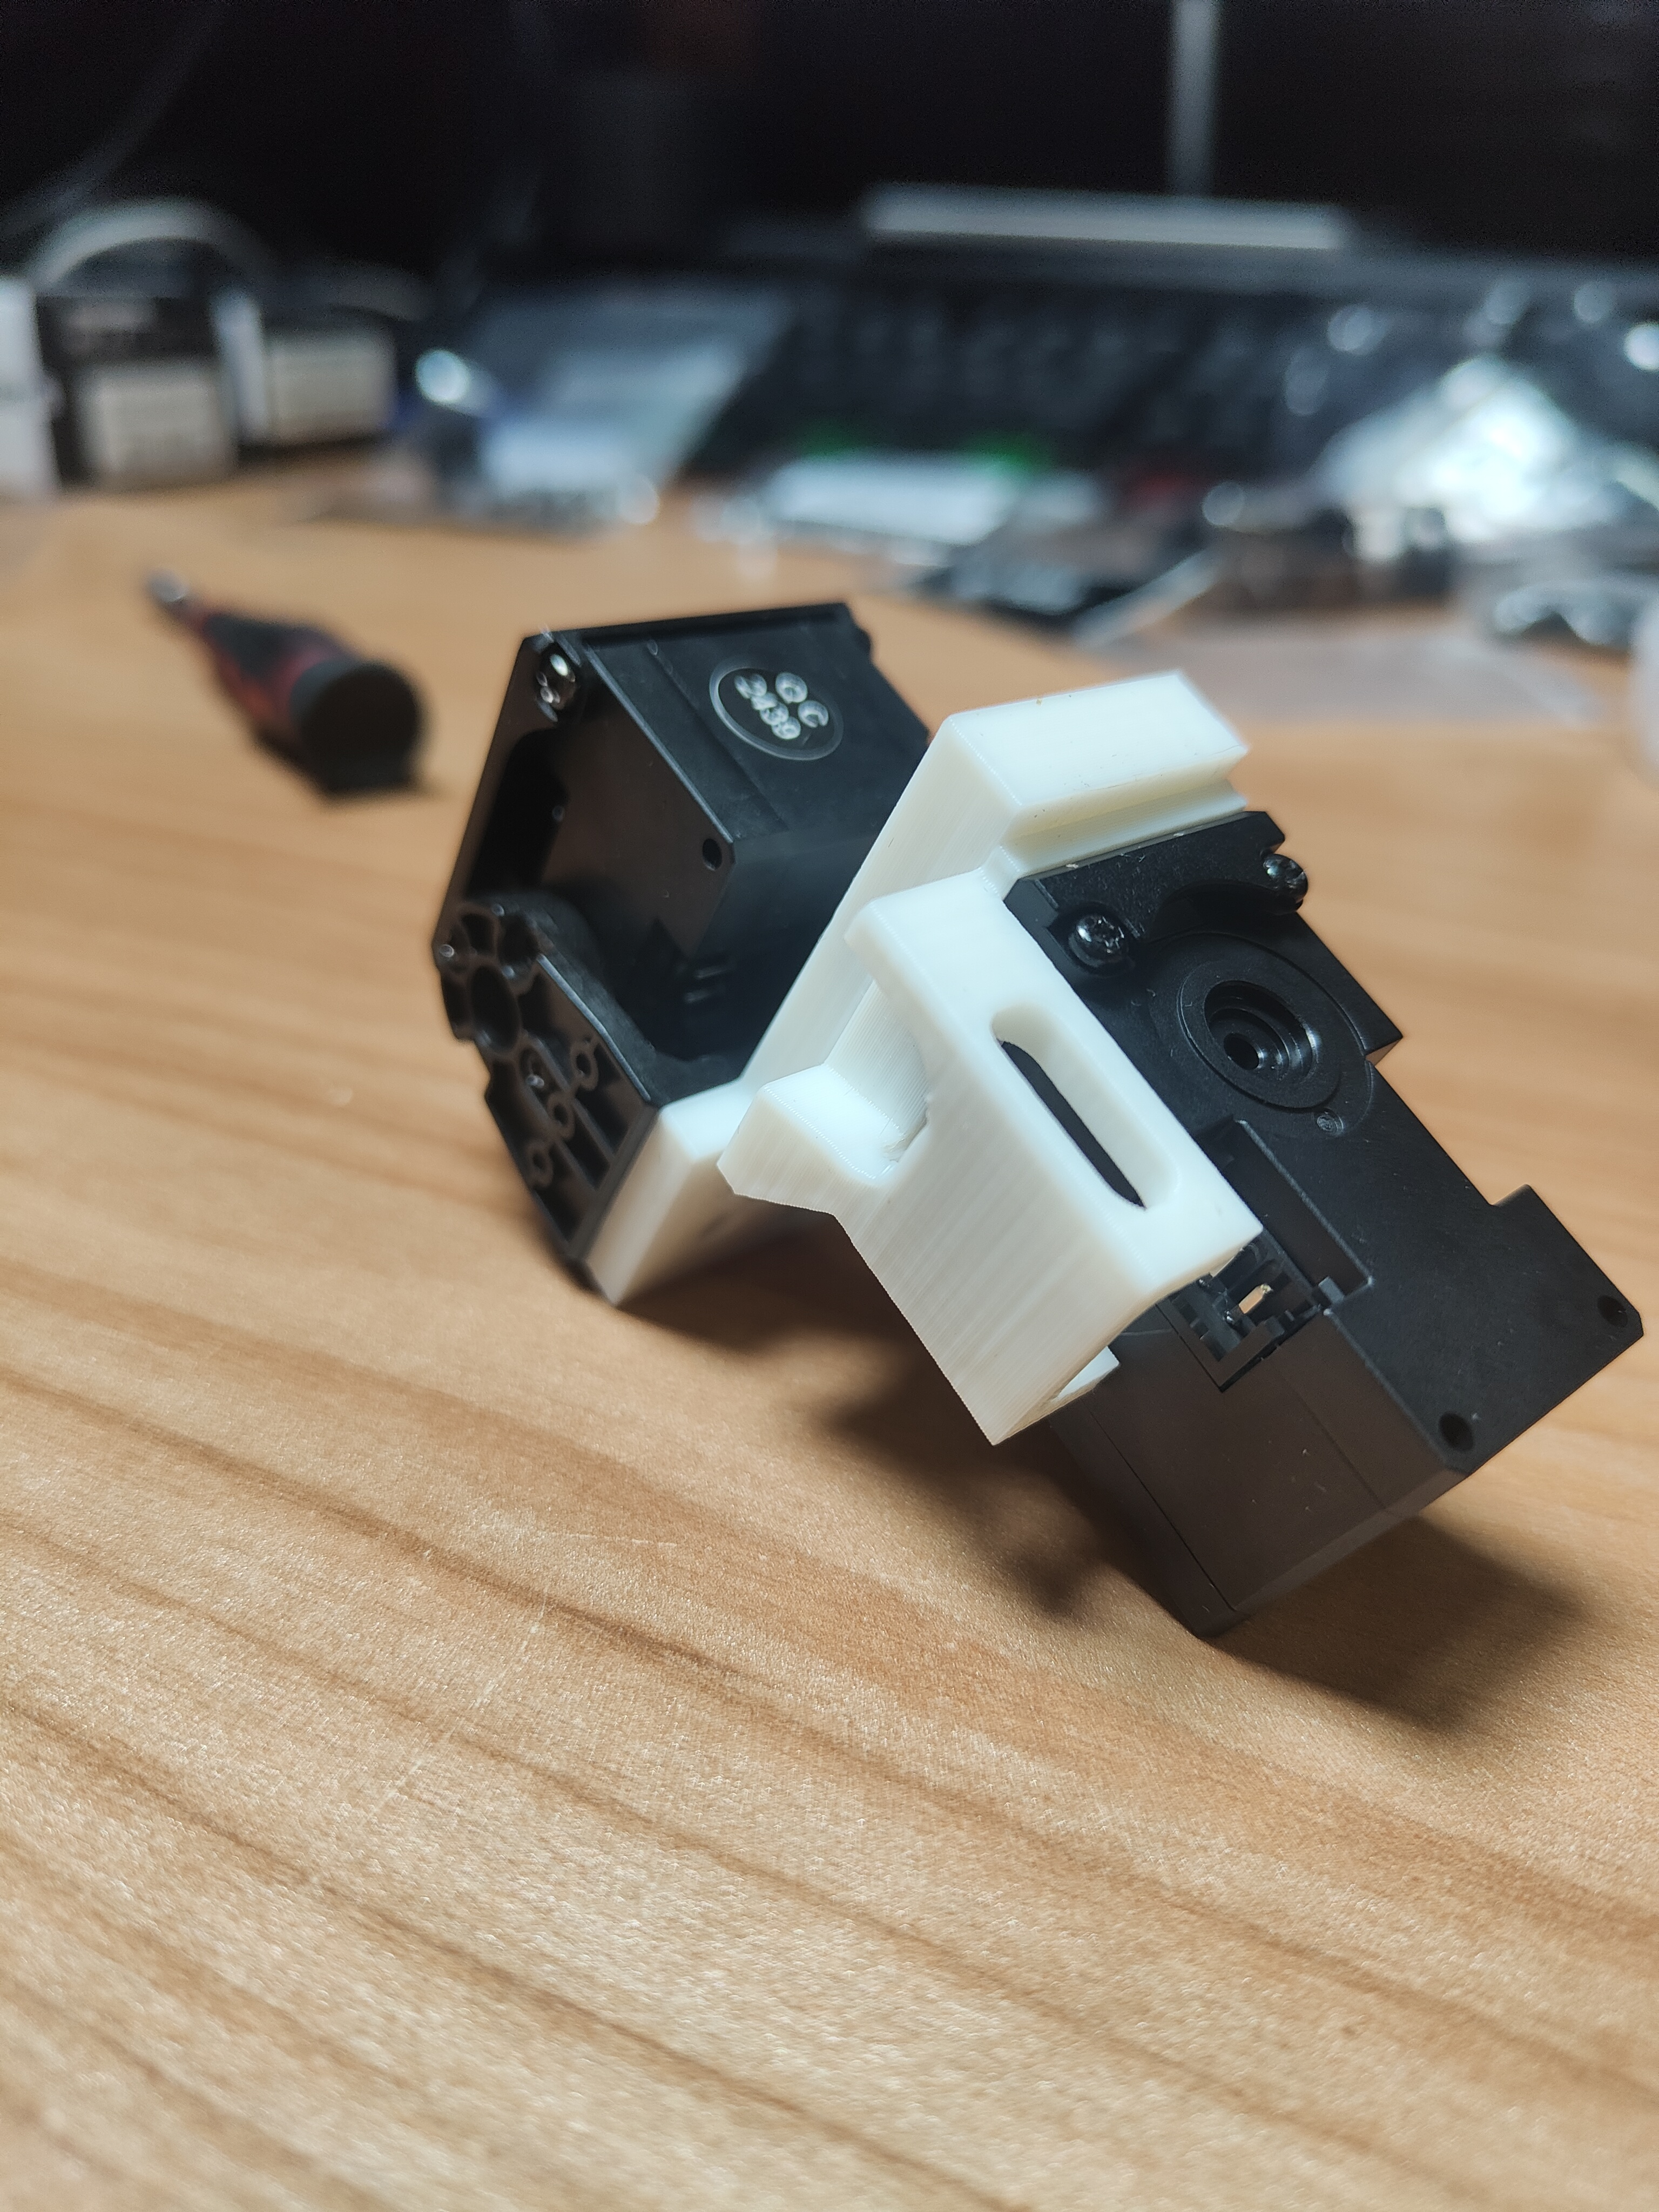
\includegraphics[width=0.25\textwidth]{figs/appendix/dedo/5.jpg} &
  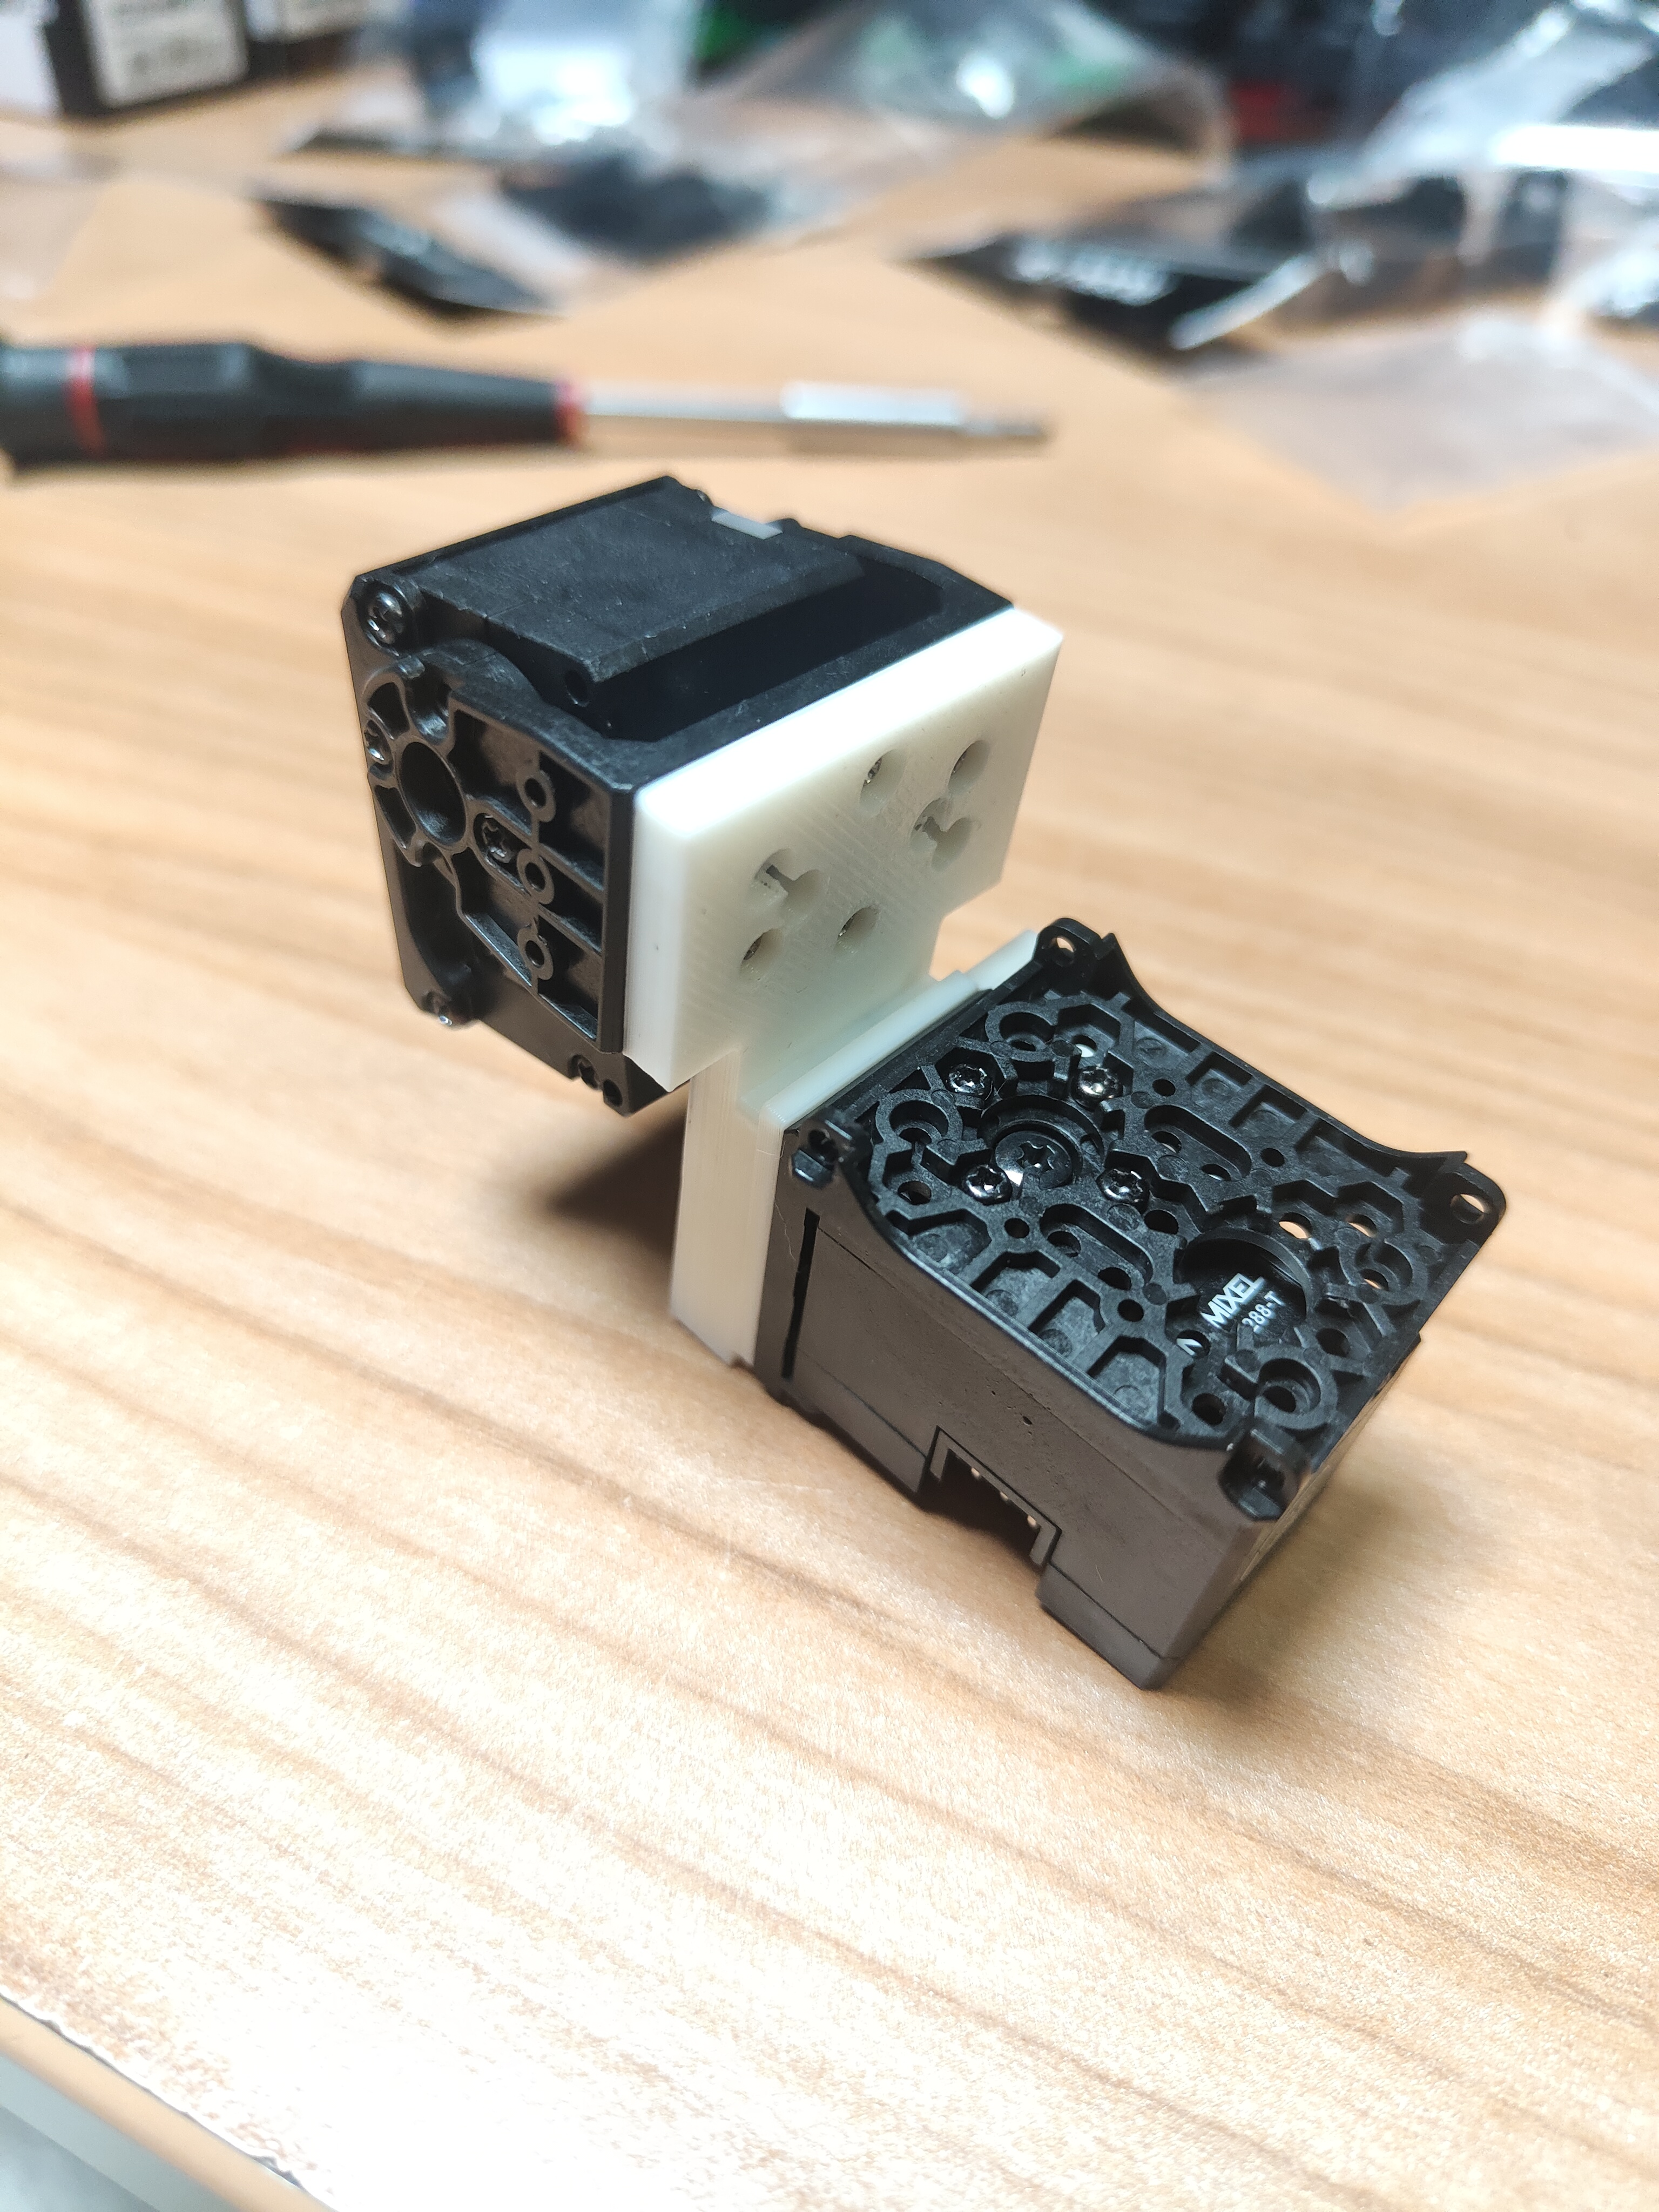
\includegraphics[width=0.25\textwidth]{figs/appendix/dedo/6.jpg} \\
  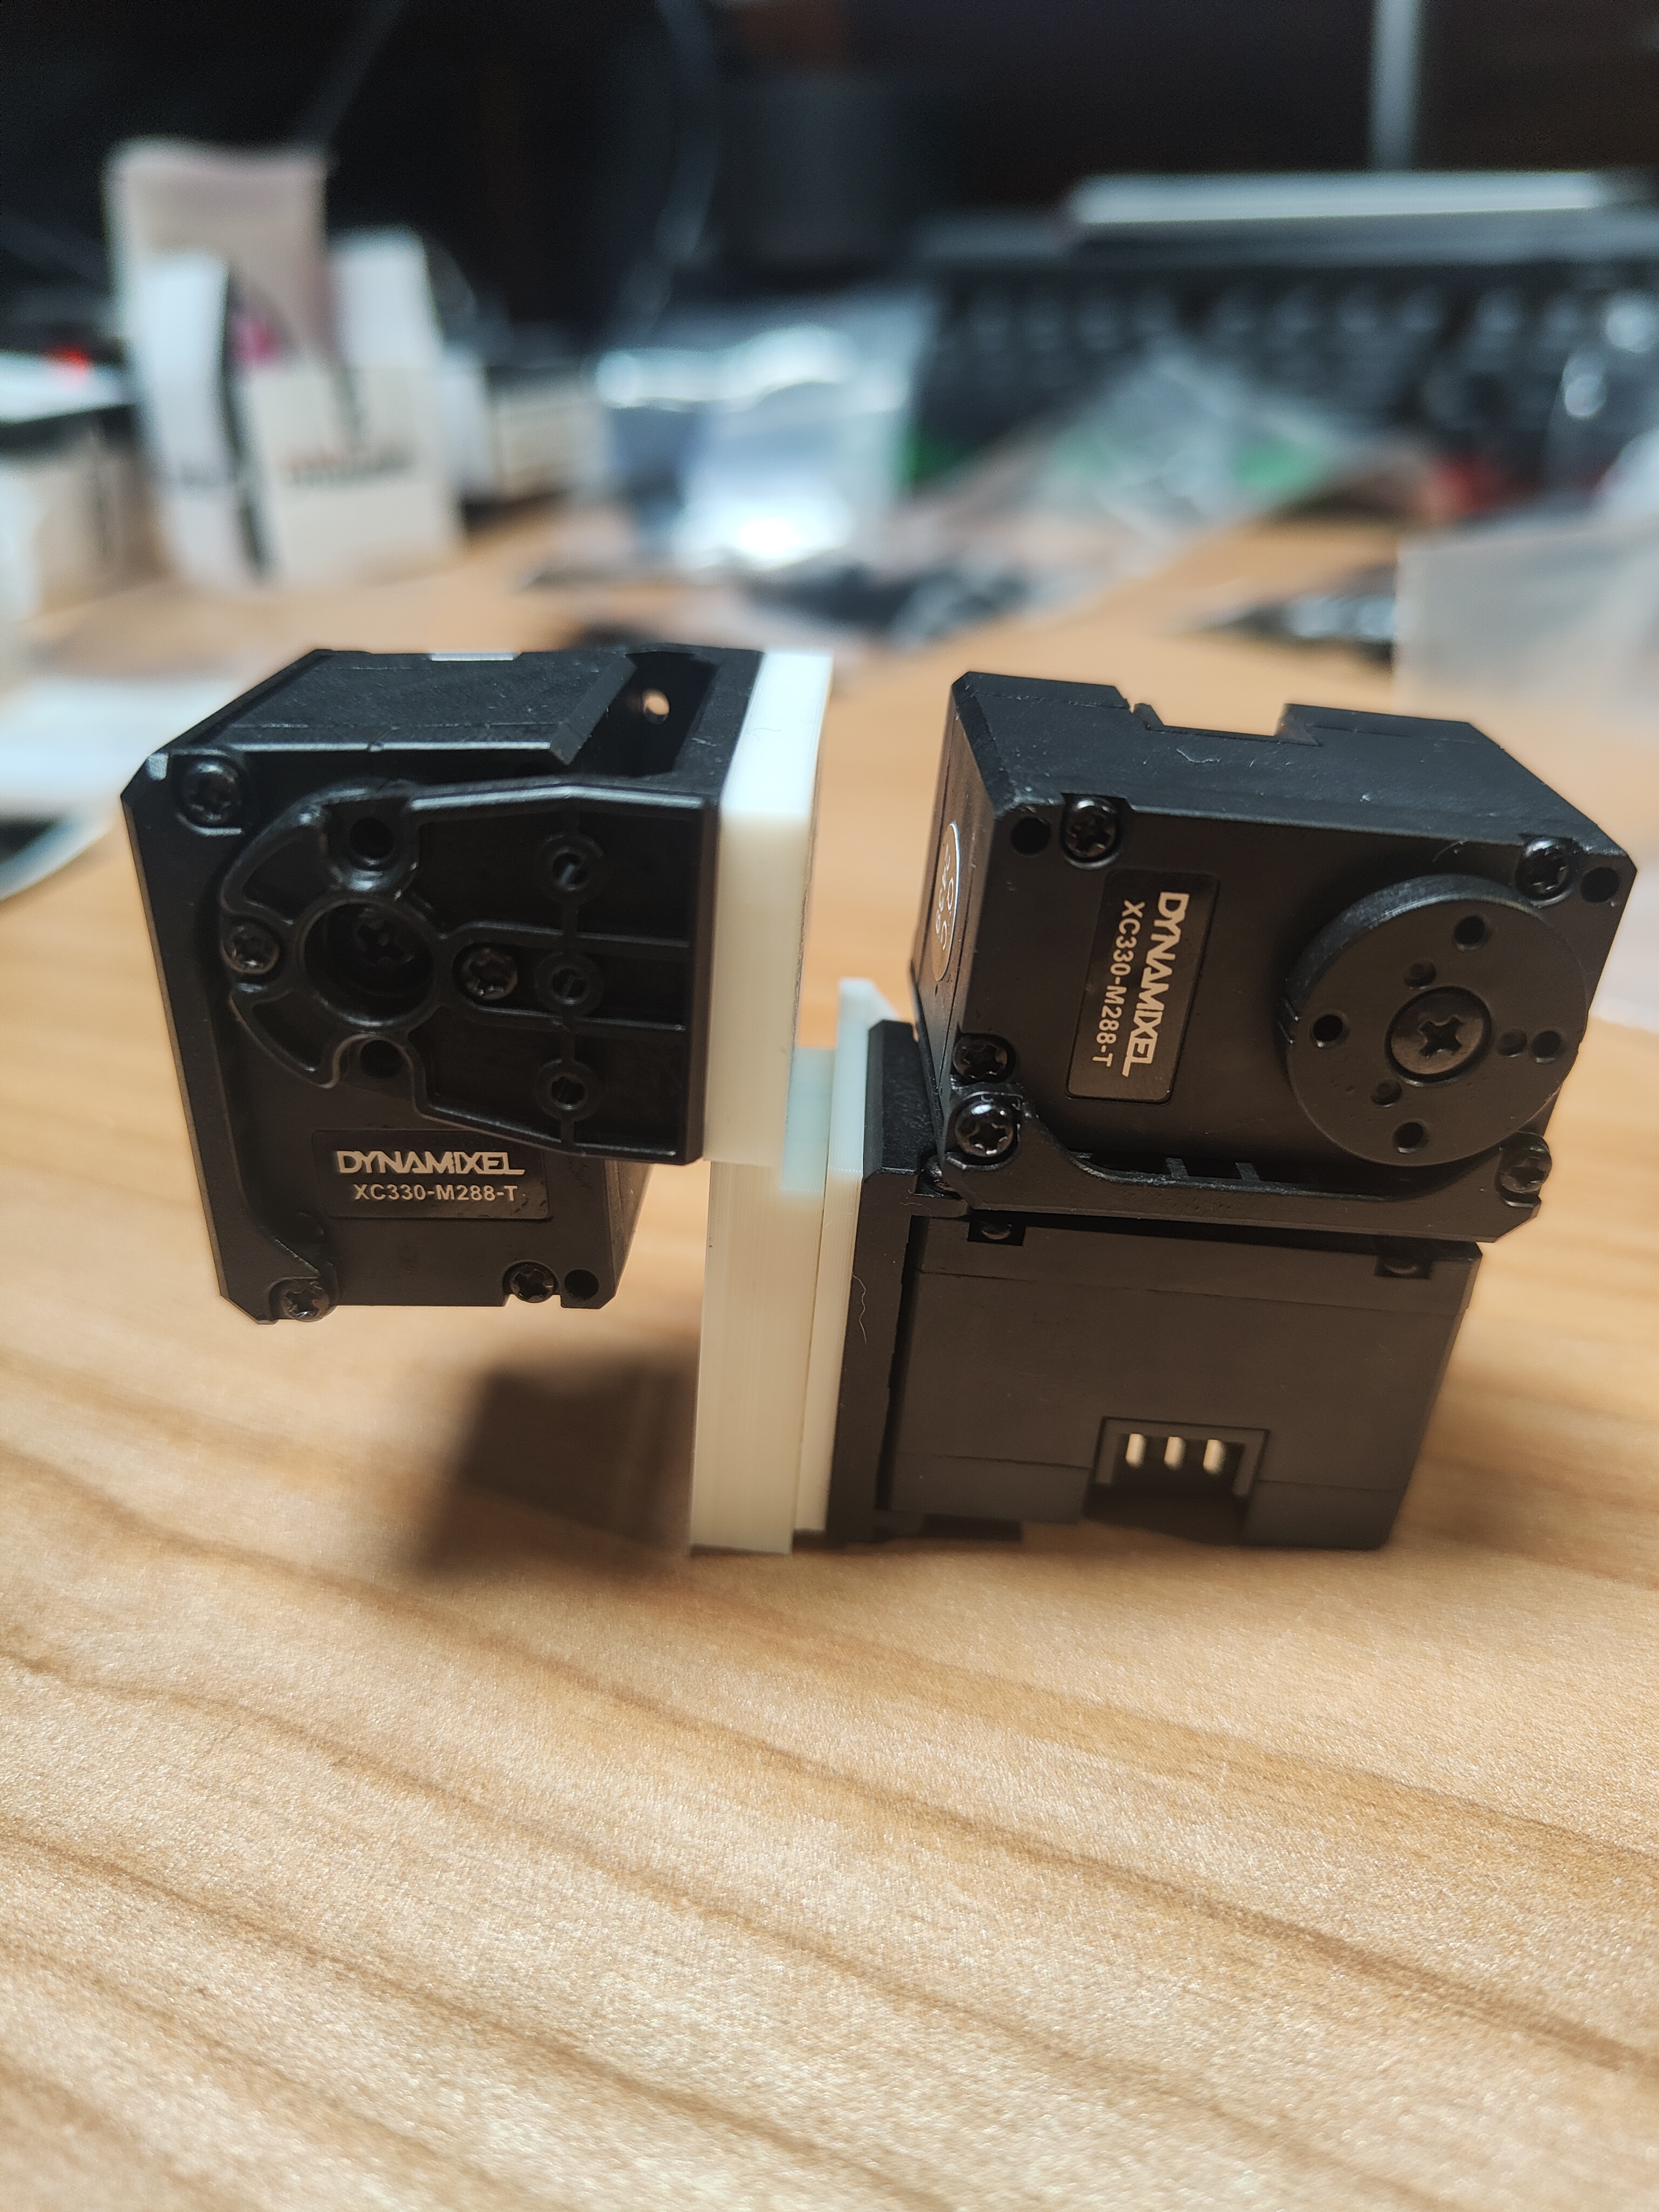
\includegraphics[width=0.25\textwidth]{figs/appendix/dedo/7.jpg} &
  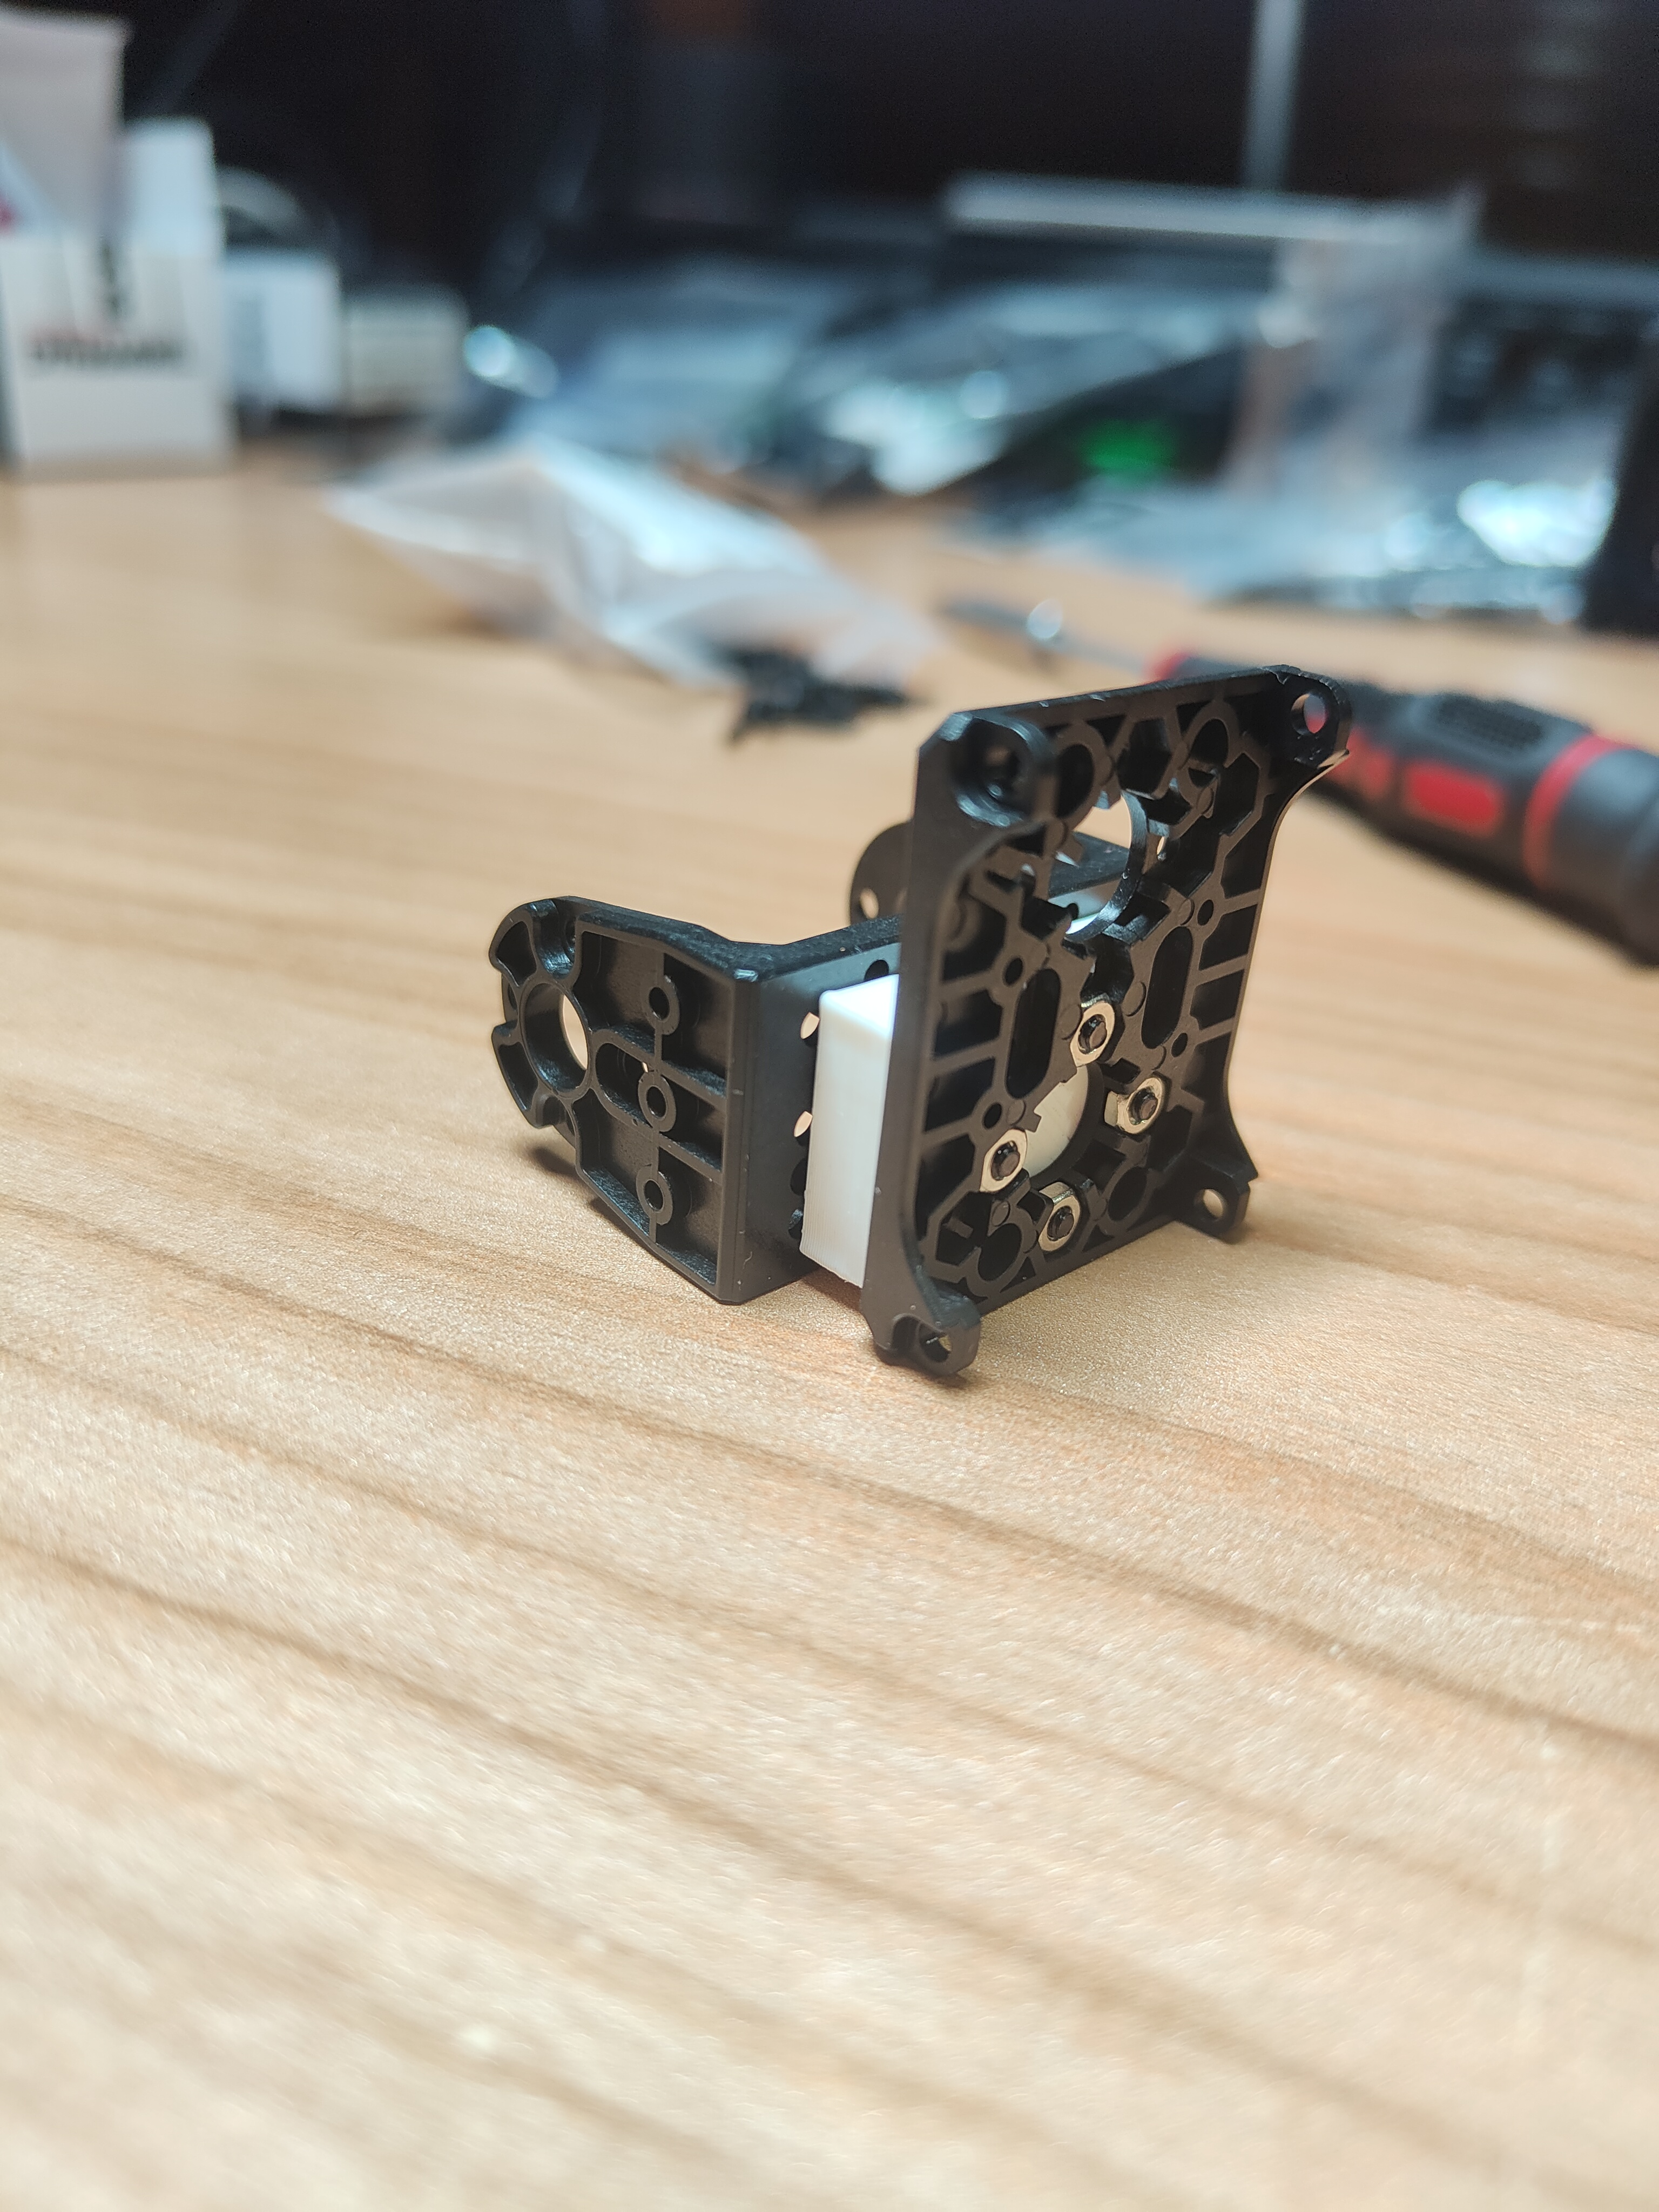
\includegraphics[width=0.25\textwidth]{figs/appendix/dedo/8.jpg} &
  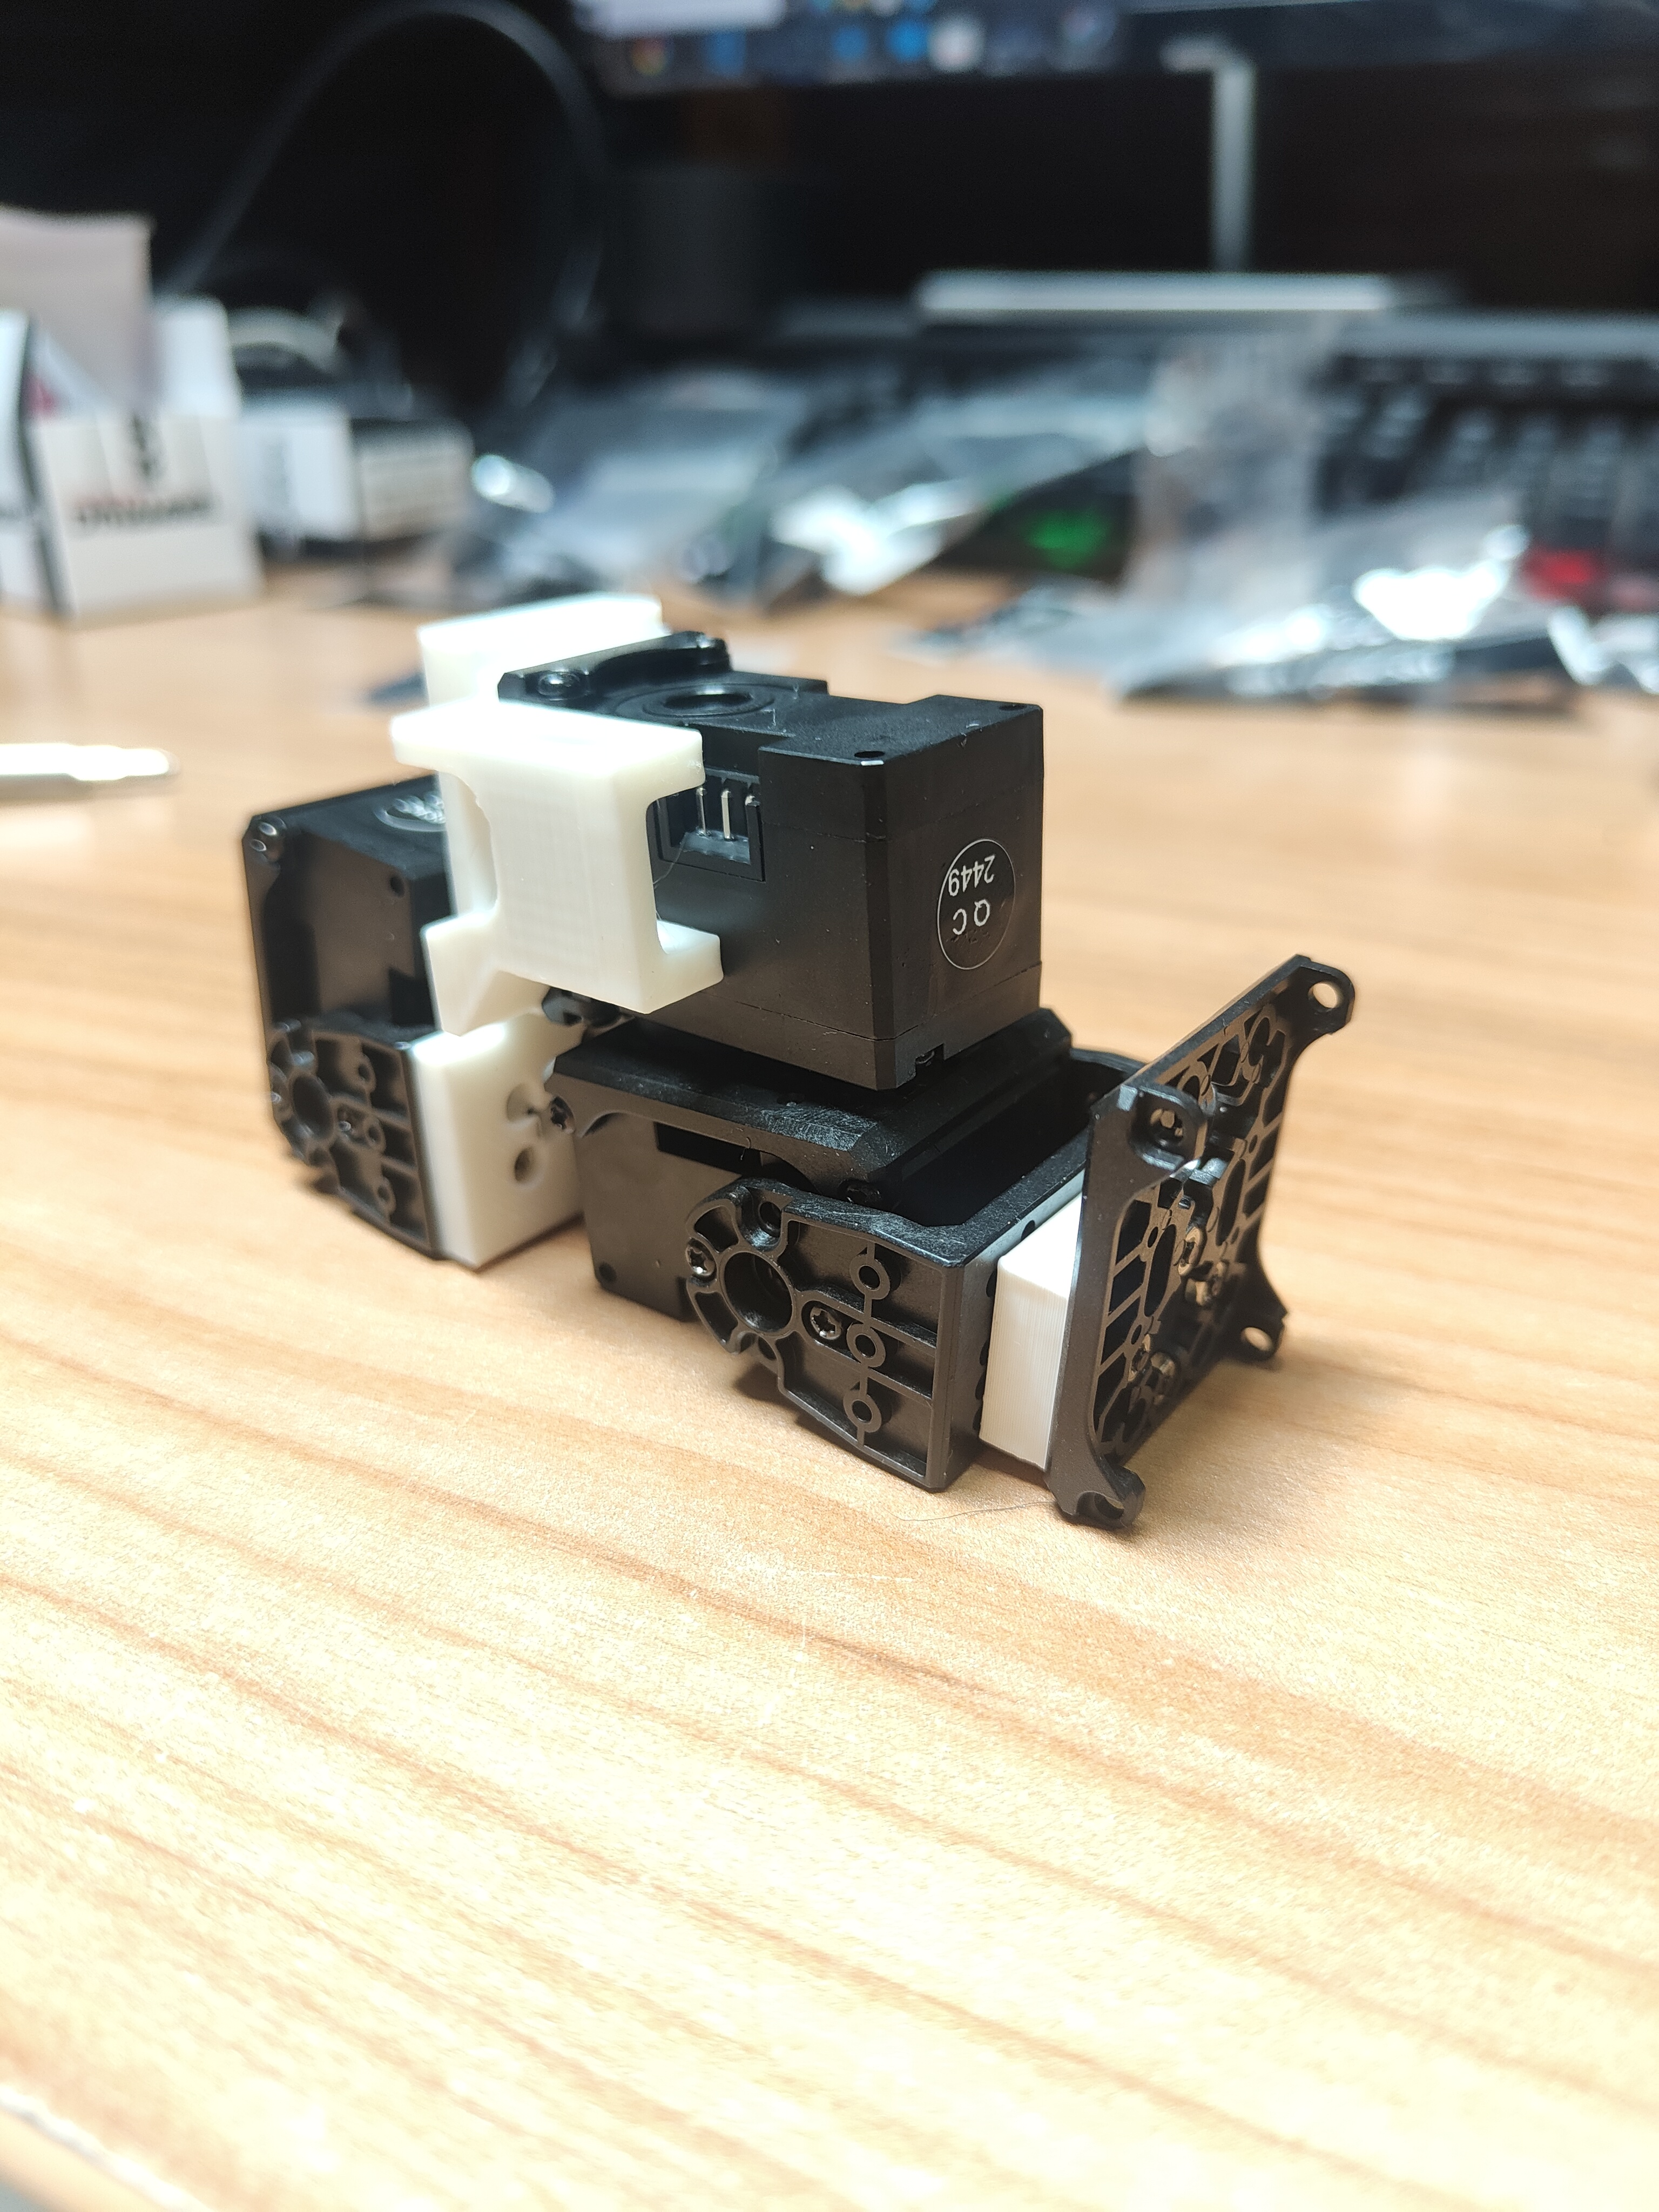
\includegraphics[width=0.25\textwidth]{figs/appendix/dedo/9.jpg} \\
  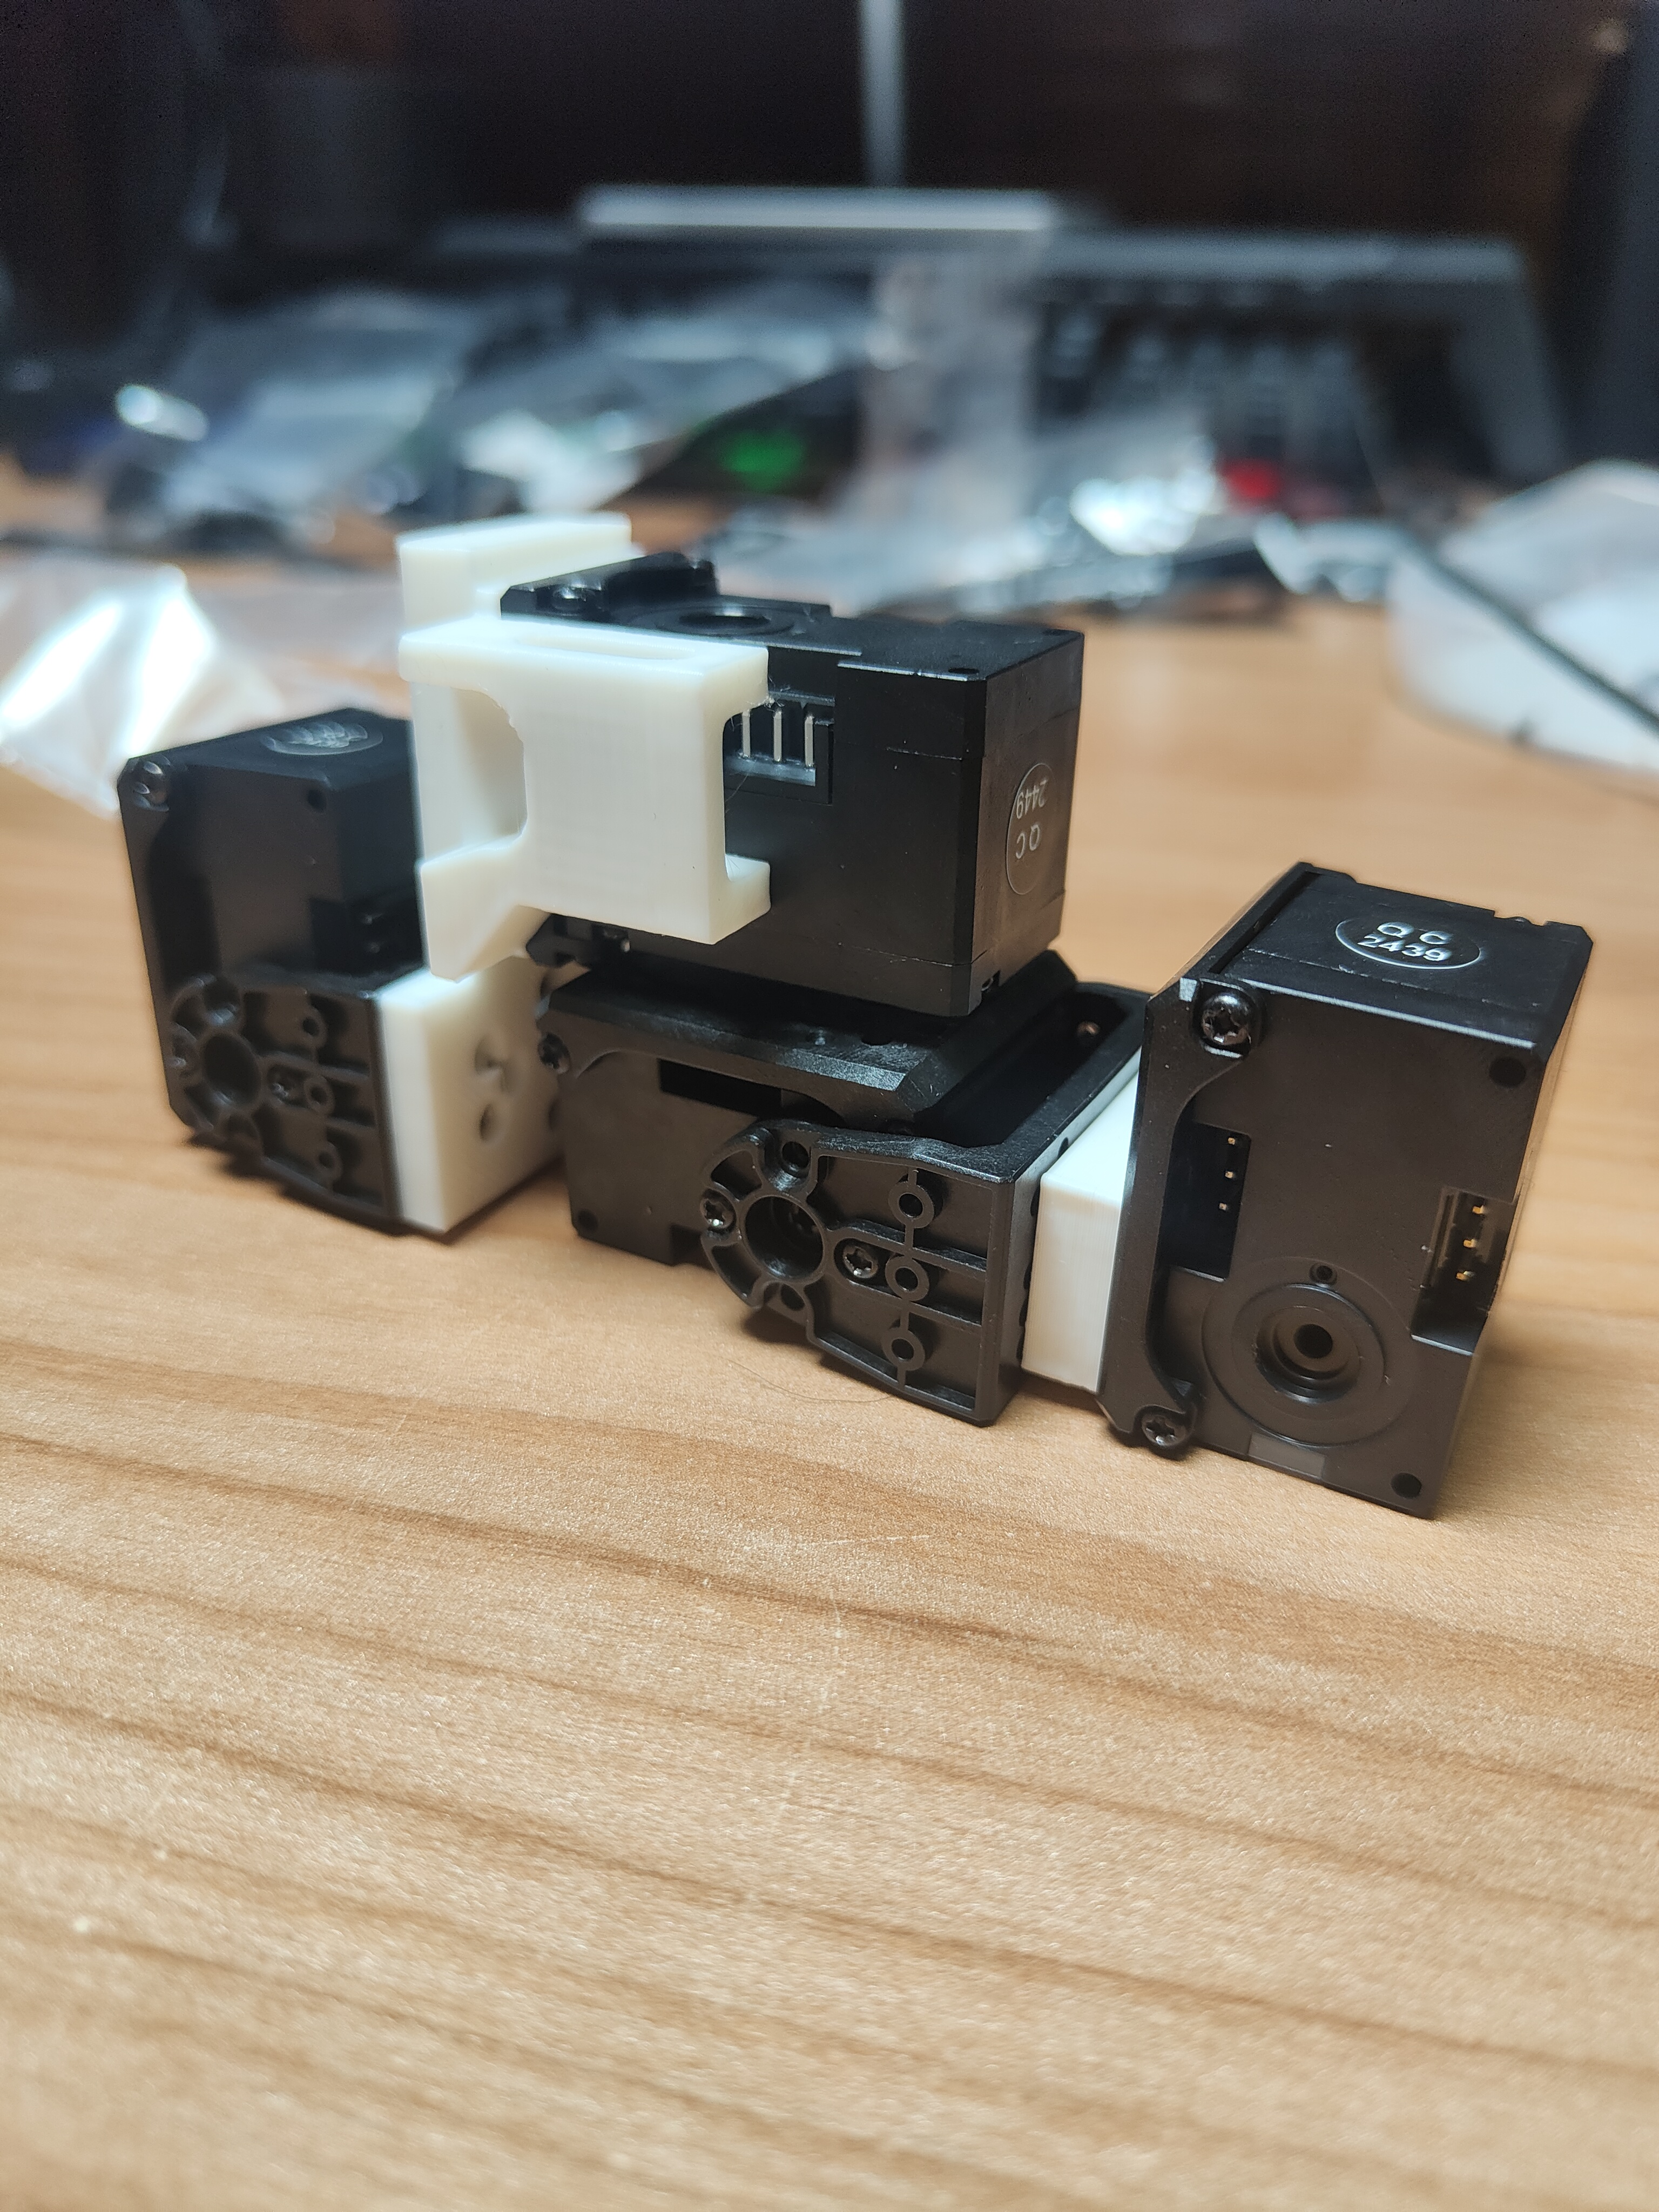
\includegraphics[width=0.25\textwidth]{figs/appendix/dedo/10.jpg} &
  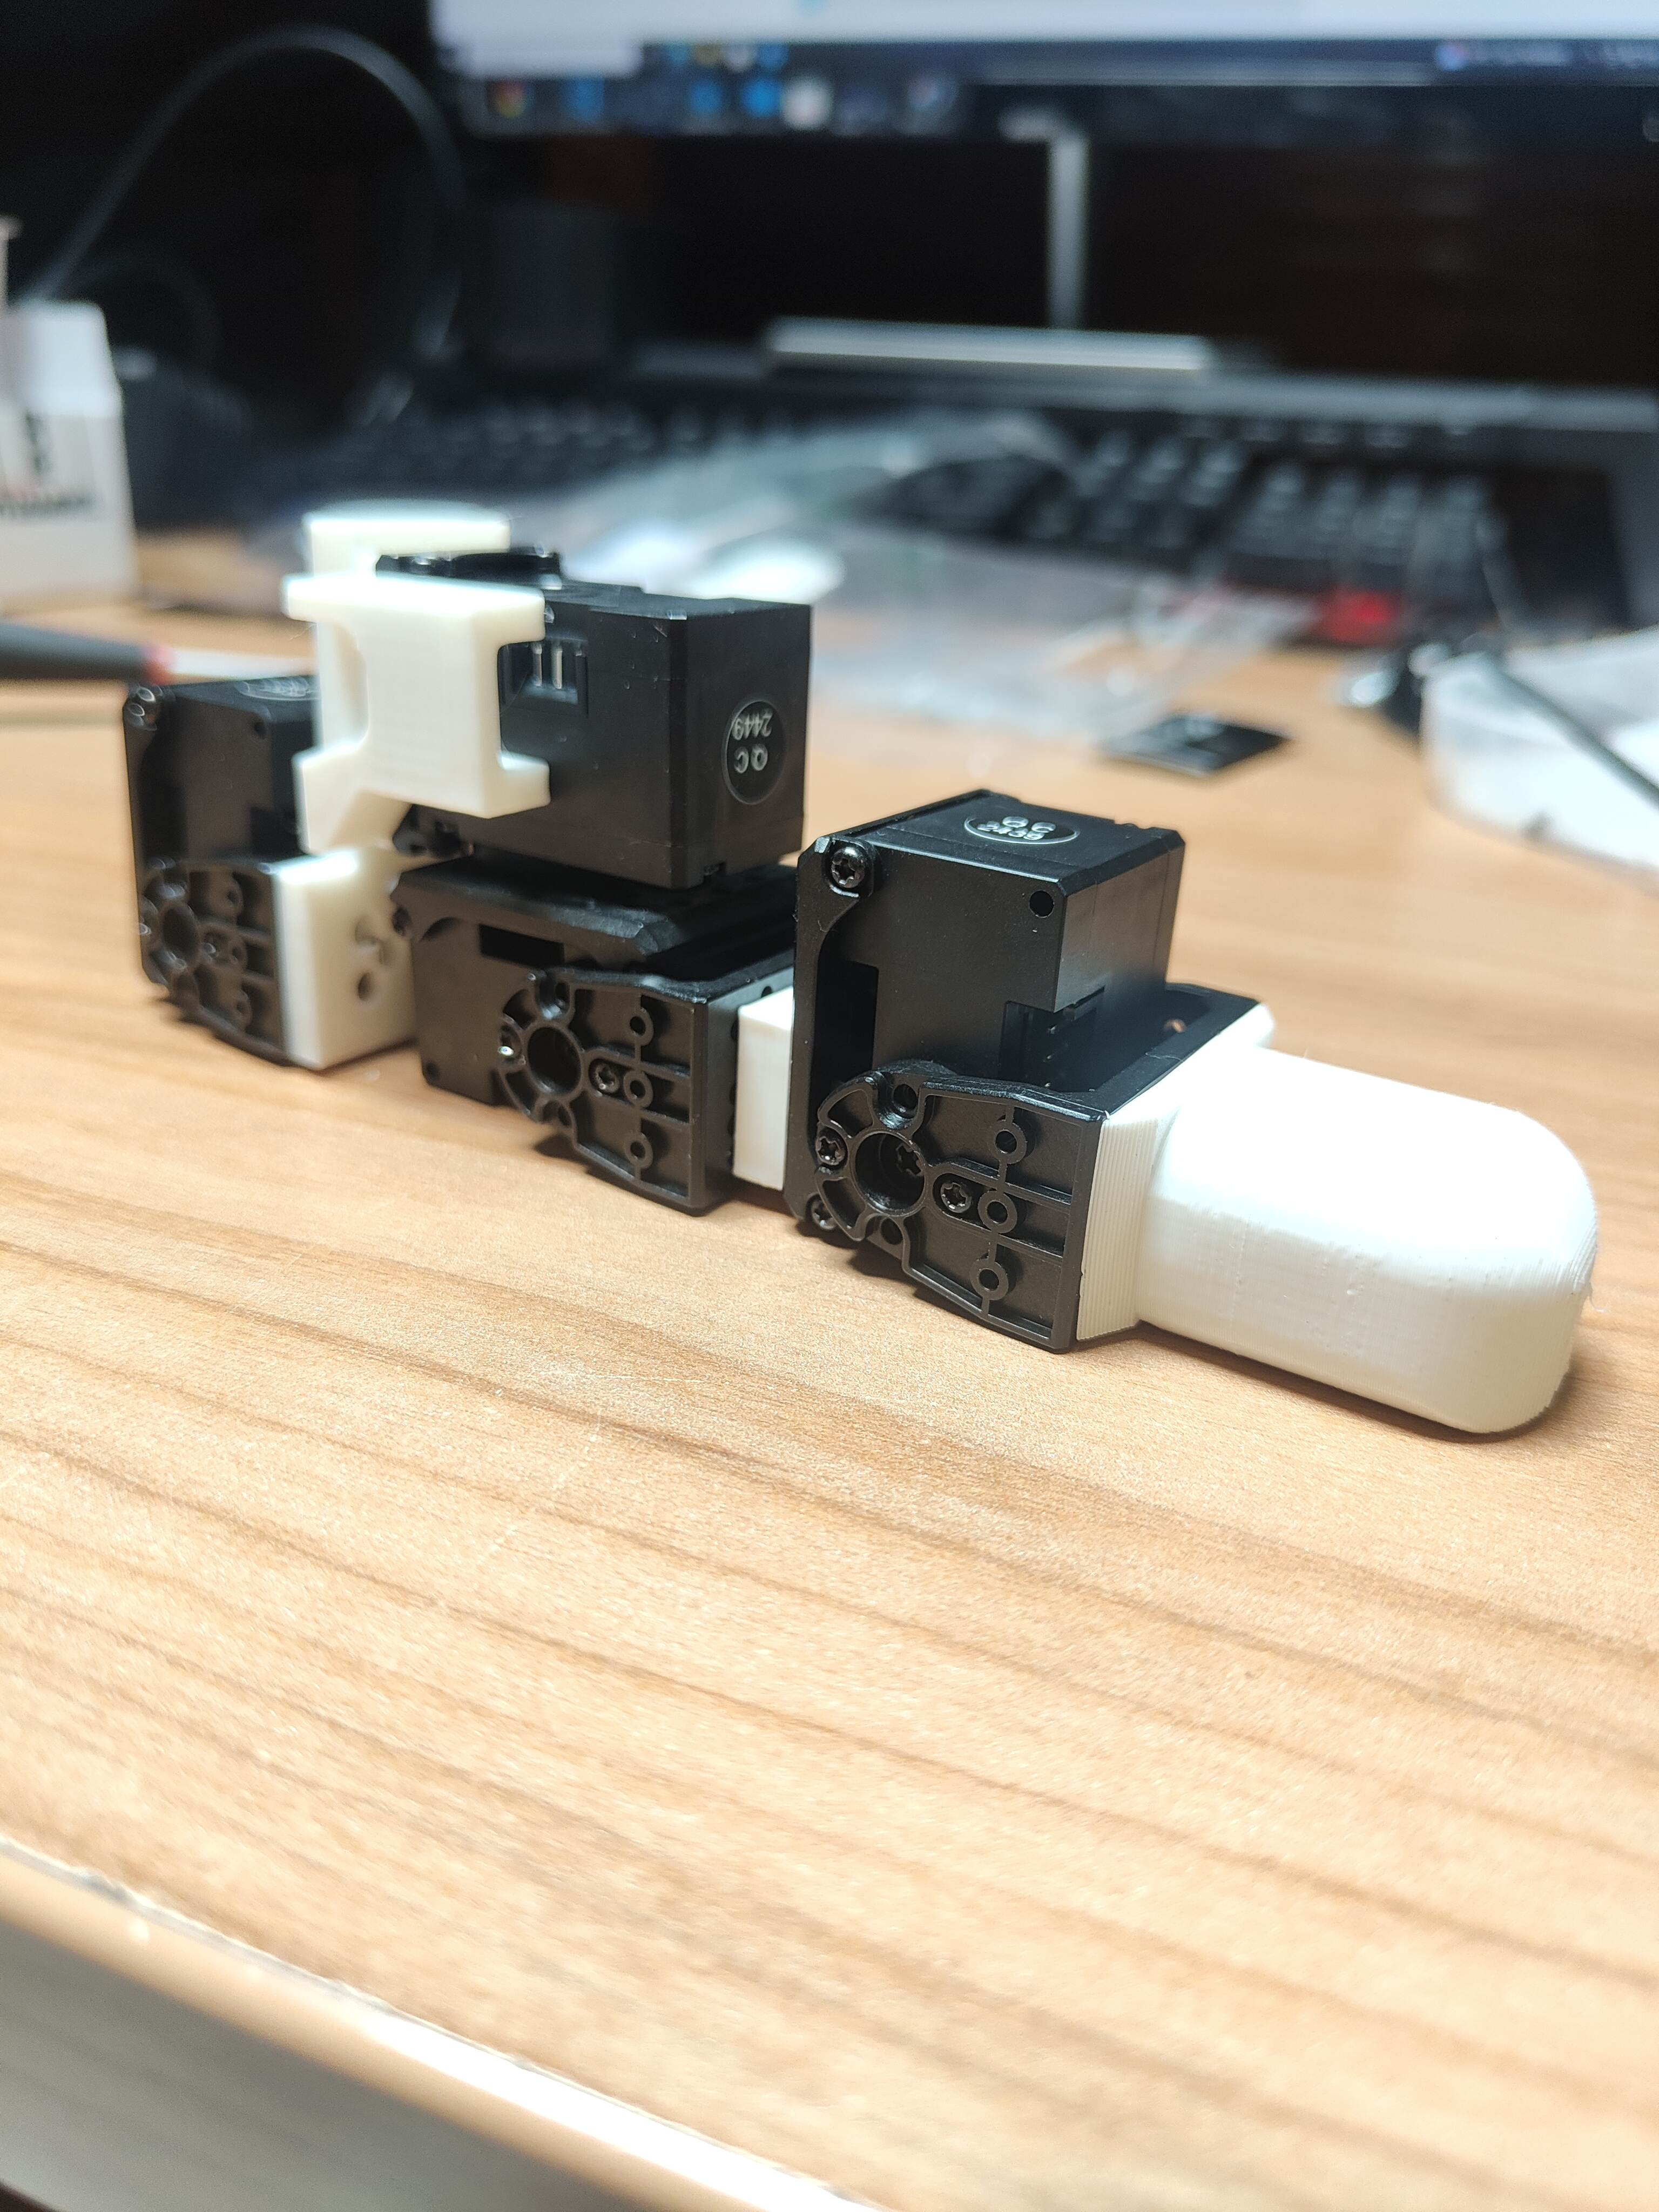
\includegraphics[width=0.25\textwidth]{figs/appendix/dedo/11.jpg} &
\end{tabular}
\caption{Fotografias sequenciais da montagem do dedo referente ao dedo indicador, médio ou anelar}
\end{figure}

\label{appendix:montagem_dedo}

\subsection{Hiperligações}

\label{appendix:videos}

\section{Testes realizados com um dedo}

\subsection{Teste com duas velocidades diferentes}

\begin{figure}[H]
\centering
\begin{tabular}{ccc}
  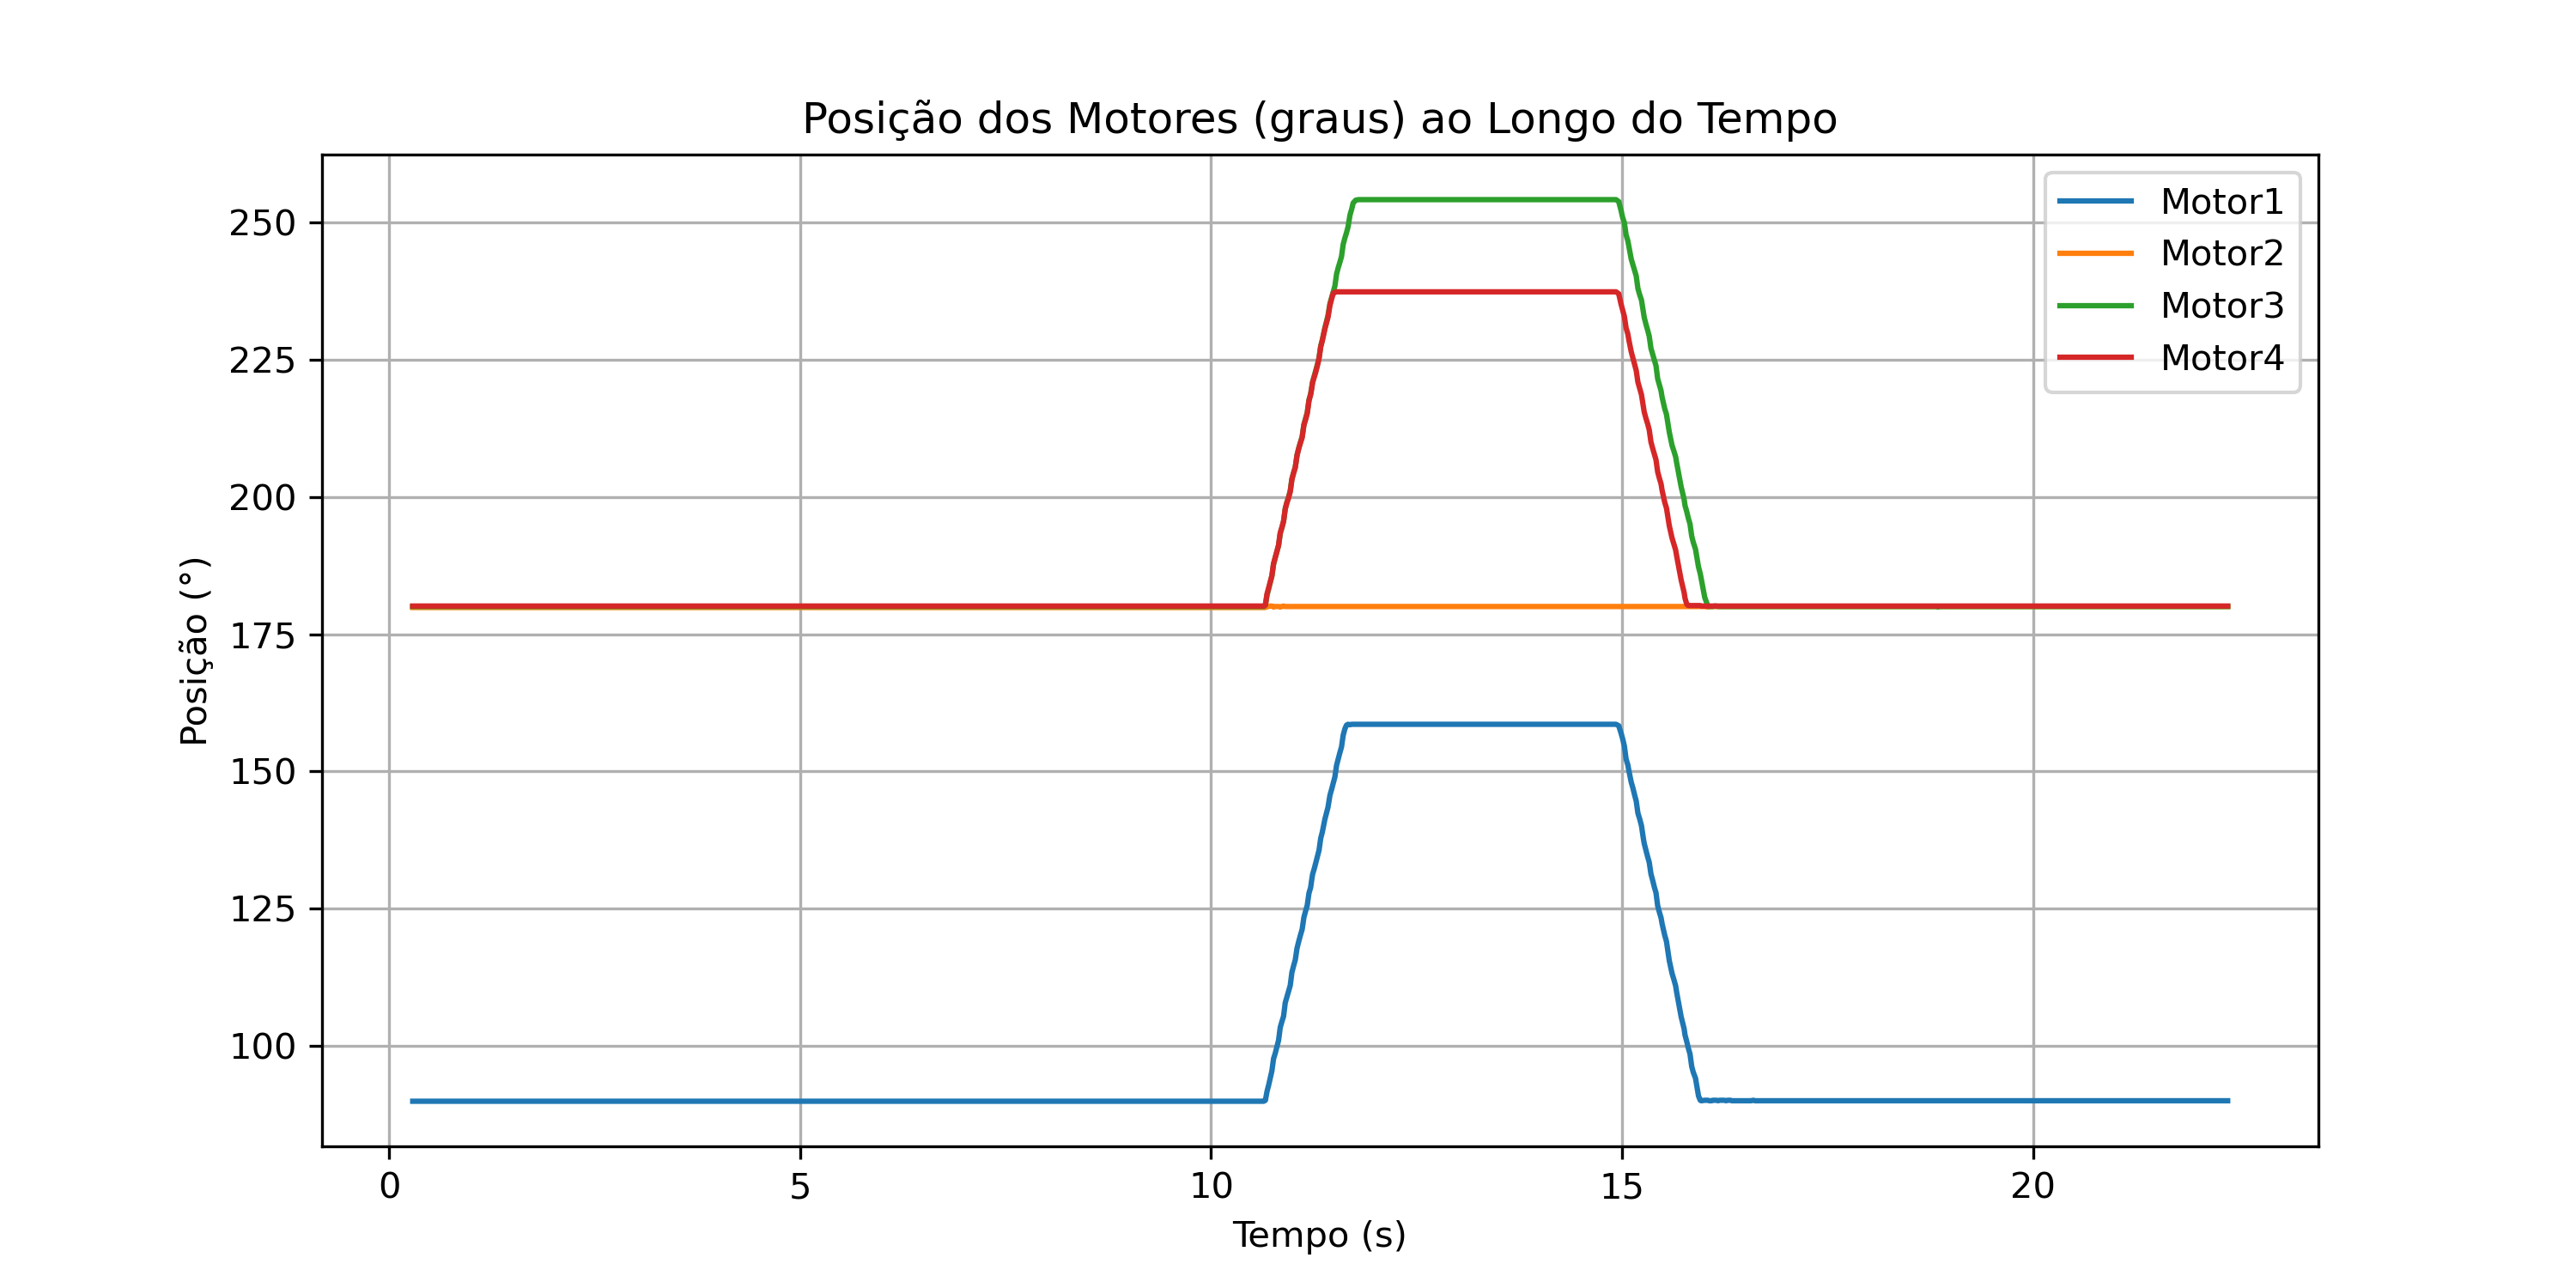
\includegraphics[width=0.5\textwidth]{figs/appendix/teste_velocidades/finger_positions_vel50.png} &
  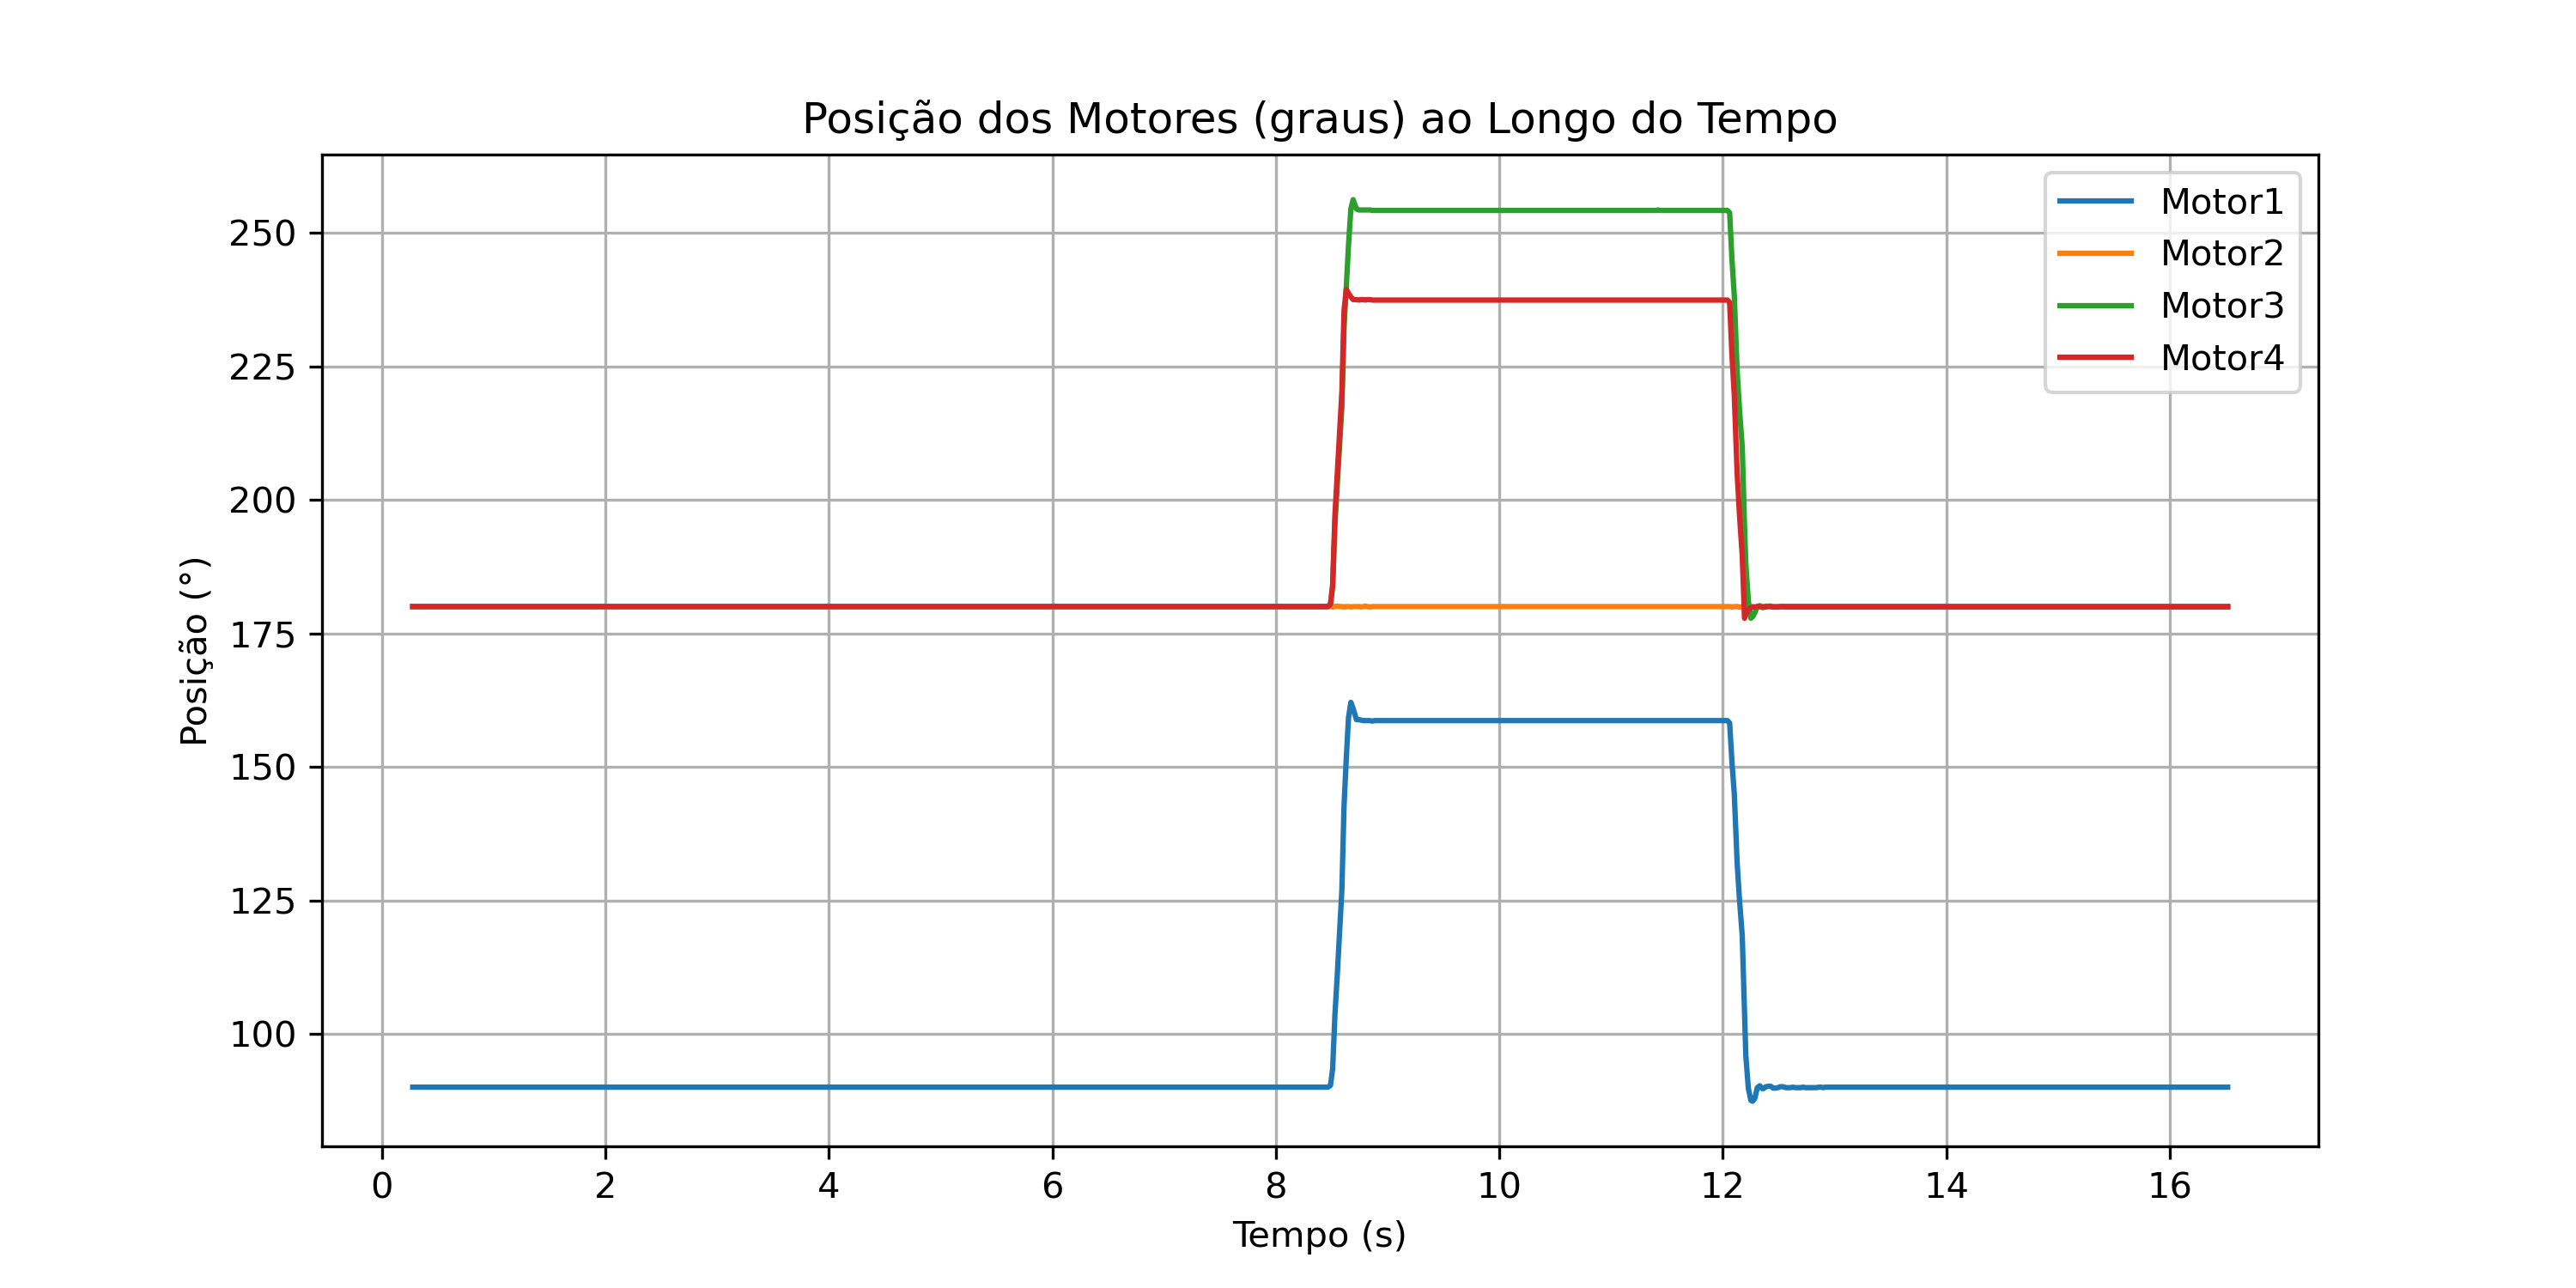
\includegraphics[width=0.5\textwidth]{figs/appendix/teste_velocidades/finger_positions_vel1000.png} \\
  \includegraphics[width=0.5\textwidth]{figs/appendix/teste_velocidades/finger_velocities_vel50.png} &
  \includegraphics[width=0.5\textwidth]{figs/appendix/teste_velocidades/finger_velocities_vel1000.png} \\
  \includegraphics[width=0.5\textwidth]{figs/appendix/teste_velocidades/finger_currents_vel50.png} &
  \includegraphics[width=0.5\textwidth]{figs/appendix/teste_velocidades/finger_currents_vel1000.png} \\
\end{tabular}
\caption{Gráficos da posição, velocidade e corrente consumida pelos motores de um dedo. A coluna da esquerda corresponde a uma velocidade máxima configurada de 1.2 rad/s e a coluna da direita a 23.98 rad/s.}
\end{figure}

Hiperligação para vídeo: \url{https://www.youtube.com/shorts/_3l9AzUPu9A}

\label{appendix:teste_velocidades}

\subsection{Teste com obstáculo em posições diferentes}

\begin{figure}[H]
\centering
\begin{tabular}{ccc}
  \includegraphics[width=0.33\textwidth]{figs/appendix/teste_pos_obst/finger_pos_vel50_obs_motor1.png} &
  \includegraphics[width=0.33\textwidth]{figs/appendix/teste_pos_obst/finger_pos_vel50_obs_motor2.png} &
  \includegraphics[width=0.33\textwidth]{figs/appendix/teste_pos_obst/finger_pos_vel50_obs_ponta.png} \\
  \includegraphics[width=0.33\textwidth]{figs/appendix/teste_pos_obst/finger_vels_vel50_obs_motor1.png} &
  \includegraphics[width=0.33\textwidth]{figs/appendix/teste_pos_obst/finger_vels_vel50_obs_motor2.png} &
  \includegraphics[width=0.33\textwidth]{figs/appendix/teste_pos_obst/finger_vels_vel50_obs_ponta.png} \\
  \includegraphics[width=0.33\textwidth]{figs/appendix/teste_pos_obst/finger_currs_vel50_obs_motor1.png} &
  \includegraphics[width=0.33\textwidth]{figs/appendix/teste_pos_obst/finger_currs_vel50_obs_motor2.png} &
  \includegraphics[width=0.33\textwidth]{figs/appendix/teste_pos_obst/finger_currs_vel50_obs_ponta.png} \\
\end{tabular}
\caption{Gráficos da posição, velocidade e corrente consumida pelos motores de um dedo, em diferentes cenários de obstrução. A coluna da esquerda representa a presença de um obstáculo junto ao motor mais próximo da base do dedo, a coluna central refere-se à obstrução a meio do dedo, e a coluna da direita corresponde à interferência na ponta do dedo.}
\end{figure}

Hiperligação para vídeo: \url{https://www.youtube.com/shorts/Qy4lXXRUP4Q}

\label{appendix:teste_posições_obstaculos}


\end{document}
